\documentclass[11pt]{article}
% Shared preamble for lyapunov.tex.  Section files must not define macros; add them here.
\usepackage[a4paper,margin=2.5cm]{geometry}
\usepackage{amsmath,amssymb,amsthm,mathtools}
\usepackage{bm}
\usepackage{booktabs,tabularx,longtable,array}
\usepackage{graphicx}
\usepackage[table]{xcolor}
\usepackage{enumitem}
\usepackage{caption}
\usepackage{microtype}
\usepackage{url}
\usepackage[hypertexnames=false,colorlinks=true,linkcolor=blue!50!black,citecolor=green!35!black,urlcolor=blue!50!black]{hyperref}

\graphicspath{{../results/}}
\numberwithin{equation}{section}
\setlist{itemsep=2pt,topsep=4pt}
\renewcommand{\arraystretch}{1.15}
\newcolumntype{Y}{>{\raggedright\arraybackslash}X}

% ---------------------------------------------------------------- results with fixed labels
% \begin{thm}{Theorem}{A}[optional title] ... \end{thm}   (italic body: theorems, propositions, lemmas,
%                                                           corollaries, conjectures)
% \begin{rmk}{Remark}{H.7a}[optional title] ... \end{rmk}  (upright body: remarks, definitions, assumptions,
%                                                           examples)
\newcommand{\reslabel}{}
\theoremstyle{plain}
\newtheorem*{genericthm}{\reslabel}
\theoremstyle{definition}
\newtheorem*{genericrmk}{\reslabel}
\theoremstyle{plain}
\NewDocumentEnvironment{thm}{m m o}
  {\renewcommand{\reslabel}{#1 #2}\IfNoValueTF{#3}{\begin{genericthm}}{\begin{genericthm}[#3]}}
  {\end{genericthm}}
\NewDocumentEnvironment{rmk}{m m o}
  {\renewcommand{\reslabel}{#1 #2}\IfNoValueTF{#3}{\begin{genericrmk}}{\begin{genericrmk}[#3]}}
  {\end{genericrmk}}

% Status line and verification pointers.
\newcommand{\status}[1]{\par\smallskip\noindent{\small\textsf{\textbf{Status.}} #1}\par\smallskip}
\DeclareUrlCommand\code{\urlstyle{tt}}
\newcommand{\checkedby}[1]{\par\noindent{\small\textsf{Checked by:} #1}\par\smallskip}

% ---------------------------------------------------------------- notation
\newcommand{\R}{\mathbb{R}}
\newcommand{\N}{\mathbb{N}}
\newcommand{\E}{\mathbb{E}}
\newcommand{\Prob}{\mathcal{P}}
\newcommand{\norm}[1]{\lVert #1\rVert}
\newcommand{\abs}[1]{\lvert #1\rvert}
\newcommand{\ip}[2]{\langle #1,\, #2\rangle}
\newcommand{\dd}{\,\mathrm{d}}
\newcommand{\Proj}{\operatorname{Proj}_K}
\newcommand{\ThK}{\Theta_K}
\newcommand{\ThKe}{\Theta_K^{\varepsilon}}
\newcommand{\Ginv}{G^{-1}}
\newcommand{\WG}{W_{G^{-1}}}
\newcommand{\VOT}{V_{\mathrm{OT}}}
\newcommand{\fhat}{\hat f}
\newcommand{\Aavg}{(\mathfrak{A})}
\newcommand{\Lsig}{(\mathrm{L}_\sigma)}
\newcommand{\RMS}{\operatorname{RMS}}
\newcommand{\diam}{\operatorname{diam}}
\newcommand{\supp}{\operatorname{supp}}
\newcommand{\Ent}{\operatorname{Ent}}
\newcommand{\KL}{\operatorname{KL}}
\newcommand{\Lip}{\operatorname{Lip}}
\newcommand{\tr}{\operatorname{tr}}
\newcommand{\sgn}{\operatorname{sgn}}
\newcommand{\clip}{\operatorname{clip}}
\newcommand{\Id}{\mathrm{Id}}
\newcommand{\T}{\top}


\title{\textbf{Self-Adaptive Kernels as Evolving Measures:\\ Transport Adaptive Control}\\[6pt]
\large Mathematical Foundations of Self-Adaptive Kernels, version 2: a complete mathematical treatment}
\author{Delhi Technological University}
\date{October 2026}

\begin{document}
\maketitle
\thispagestyle{empty}
\begin{center}
\small
\begin{minipage}{0.86\textwidth}
\textbf{Version 2.} This document supersedes version 1, \emph{Mathematical Foundations of Self-Adaptive Kernels
Achieving Lyapunov Convergence}. Section~\ref{sec:version1} states what survived from version 1 and what was
withdrawn. This is research in progress and has not been peer reviewed. Code, tests, experiments and review records:
\url{https://github.com/Dutta-06/Lyapunov-Convergence-Kernels-Showcase}.\\[4pt]
Copyright \copyright\ 2026 Odwitiyo Dutta. All rights reserved.
\end{minipage}
\end{center}

% Abstract
\begin{abstract}
This is a complete mathematical treatment of adaptive tracking control with Gaussian radial-basis-function
(RBF) networks whose weights, centres and widths are adapted online. Part~I is the projection-based adaptive RBF
controller of version~1. An audit found its stability argument to be a correct but standard composition of known
results, with two claims wrong as written (a non-convex ``projection'' for centre separation and an
implicit-function-theorem argument that is not a proof); it contains no new theorem. We state it with explicit
assumptions, a Hessian-free disturbance bound and an RMS bound, and list the errata to version~1. Part~II develops
transport adaptive control: the network is an empirical measure on a lifted parameter space, and the adaptive law is
its transport. Theorems A--D and F are proved; A, B, C and F are also checked by tests. Theorem~E is proved
conditional on Theorem~1 of Morgan and Narendra (1977), in the form stated in that paper's abstract; its hypotheses
were not checked against the full text. Proposition~G is formal and checked directly. Theorem~H shows that the
averaged mean-field loop with saturated features, $\sigma$-modification and dither is mean-field Langevin dynamics and
converges globally and exponentially to the regularised optimum; this is proved for the averaged system, the
reduction to it is formal, and the real loop is a conjecture. At finite gain the averaged loop is in general not a
gradient flow of any free energy in the $\WG$ metric: Proposition~H.7 (frozen-measure part proved) exhibits a
semi-gradient term, whose performative defect is non-reciprocal in the checked instances ($n = 1, 2$), and an
orbit-area circulation kernel ($n \ge 2$). With a second-order averaging term they predict a closed-loop effect for
which a targeted literature search found no precedent: traversing the reference orbit backwards changes the learned
kernels by $O(1/k_e)$, although the occupation measure is unchanged. At $k_e = 40$ the prediction matches to 3\% in
size and 11\% as a vector (cosine 0.994). Proposition~H.8, proved assuming the chain rule for the perturbed flow,
gives input-to-state stability of the averaged system.
\end{abstract}


\clearpage
\tableofcontents
\clearpage

% Front matter: introduction (PARADIGM.md section 0), relation to version 1
% (lyapunov_text.txt, ASSESSMENT.md, THEORY_REVISED.md section 6, public_showcase/README.md).

\section{Introduction}\label{sec:intro}

\subsection{The idea}

An adaptive approximator with nonlinearly parametrised features can be read as an \emph{empirical measure}
$\mu = \frac1m\sum_i\delta_{\vartheta_i}$ on a lifted parameter space. Here the features are Gaussian RBF kernels
with adaptive weights, centres and widths. The adaptive law transports this measure, and the control output
$\fhat = \int\Phi\dd\mu$ is linear in $\mu$. Stability, robustness modifications, excitation, the many-kernel limit
and the slow evolution of kernel geometry all acquire formulations on Wasserstein space. So does the global
optimality of kernel placement. These formulations do not depend on how the kernels are labelled.

\subsection{Why the classical theory needs it}\label{sec:front:defects}

This work identifies two structural defects of the classical labelled analysis, that of version~1 of this manuscript
and of the literature it builds on.
\begin{itemize}
  \item The classical Lyapunov analyses depend on labels. A network that is a relabelling of the ideal has zero
    function error but a large parameter error.
  \item There is no object that describes where the kernels go, or whether their placement is good.
\end{itemize}
A third apparent defect was that constants grow with the number of kernels. It turned out to be an artefact of the
normalisation. The mean-field normalisation removes it for labelled and label-free analyses alike (Remark A.1).

\subsection{What the closed loop actually is}

\begin{itemize}
  \item At infinite feedback gain, the averaged closed loop is a Wasserstein gradient flow. With dither it is a
    mean-field Langevin dynamics (Theorem H).
  \item At finite gain it is in general \emph{not} a gradient flow of any free energy in the $\WG$ metric. This
    already holds for $n = 1$, so it is not a two-dimensional effect (Proposition H.7). The first correction has two
    parts at a frozen measure, and a third along the real loop.
    \begin{itemize}
      \item The first part is a \emph{semi-gradient} term. The adaptive law differentiates the loss on the
        closed-loop state distribution while ignoring that this distribution depends on the parameters, as in
        performative prediction. Like semi-gradient TD, the resulting update is not the gradient of any objective.
        Its performative defect is present for every $n$; for $n = 1$ it is non-reciprocal exactly when the residual
        is non-zero on the orbit (Theorem I(iii)), and it is non-reciprocal in the checked $n = 2$ instance.
      \item The second part is an antisymmetric interaction between kernels ($n \ge 2$). Its kernel is an integral
        of $\sum_k \det[\nabla\tilde\Phi_k(\vartheta), \nabla\tilde\Phi_k(\vartheta')]$ over the region that the
        reference orbit encloses (Stokes).
      \item Along the real loop, a third part comes from the parameters' oscillation within each period. It is a
        second-order averaging term (Remark H.7a).
    \end{itemize}
  \item Together these predict a new closed-loop effect: traversing the reference orbit backwards changes the learned
    kernels by $O(1/k_e)$, although the occupation measure is unchanged. At $k_e = 40$ the prediction matches to 3\%
    in size and 11\% as a vector (cosine 0.994). The vector error halves with each doubling of $k_e$
    (\code{experiments/exp_orbit_orientation.py}).
  \item The gradient structure survives as an input-to-state Lyapunov function (Proposition H.8). This reduces the
    global conjecture for the real loop to an averaging estimate.
\end{itemize}

\subsection{Conventions and verification}\label{sec:front:conventions}

\paragraph{Status labels.} Every result of Part~II is labelled \emph{proved}, \emph{formal} or
\emph{conjectural}, and the label is given in a status line after the result.
\begin{itemize}
  \item ``Proved'' means proved here. ``Formal'' means a derivation without error control.
  \item ``Checked'' means a test evaluates the statement, or every inequality in it, along simulated trajectories or
    on sampled states.
  \item The novelty column of Table~\ref{tab:front:contrib} follows the verdicts in \code{LITERATURE_TRANSPORT.md}.
\end{itemize}
In Part~I, every step of the stability argument is either proved or verified numerically by
\code{tests/test_theorem_to_code.py}.

\paragraph{Verification and review.}
\begin{itemize}
  \item Every inequality the tests can evaluate is checked numerically along simulated trajectories, and every number
    in this document is produced by a script in the accompanying repository (the experiments are in
    \code{experiments/}); no table is edited by hand.
  \item The theory went through three rounds of automated multi-agent adversarial review, the manuscript through a
    fourth that compared it line by line with the theory, the results added in version~3 (Lemma E.0, Theorems
    C$'$, D$'$, I and J, Proposition K) through a fifth, and the second increment --- the sharp slow-regime rate
    (Lemma E.0$'$), uniform-in-time propagation of chaos in the leak-dominated regime (Theorem D$''$) and the
    stationary law of the dithered finite-size loop with its non-equilibrium current (Theorem J$'$,
    Proposition J$'$.2) --- through a sixth, and the third increment --- the explicit stationary parameter spread of
    the dithered linearised loop (Corollary E.0$'$.3) and the slow-regime Lyapunov function for non-periodic
    persistently exciting regressors (Lemma E.0$''$) and uniform-in-time propagation of chaos in the learning
    regime for the averaged slow loop (Theorem D$'''$, with the finite-$m$ weight-sensitivity law of
    Proposition D$'''$.5, the real loop on a warm start of Corollary D$'''$.7, the leak's prior as a design input of
    the window, Proposition D$'''$.9, and the barycentric OT leak's mass constraint, which removes the finite-size
    floor, Proposition D$'''$.12 --- in the real loop too, where the collapsed subspace carries one $K_0$-atom orbit
    for every commensurate size, Corollary D$'''$.14 and Proposition D$'''$.15, and Theorem J holds uniformly in the
    number of kernels in the per-particle norm, Theorem D$'''$.18, while a soft (entropic) mass constraint equalises
    the masses only down to a critical excess, Proposition D$'''$.20; and the mass-constrained energy satisfies a
    Polyak--{\L}ojasiewicz inequality whose constant does not depend on the number of kernels, which gives a
    measure-level basin with an exponential rate and, at the nearest-atom leak, explains the floor as a spurious
    minimum at every admissible count vector, Theorem D$'''$.21) --- through a seventh (the first two) and an eighth
    to a sixteenth (the third), and the fourth increment --- adaptive priors and the floor removal (Theorem
    D$'''$.23, Proposition D$'''$.24, the gauge of Proposition D$'''$.28, the projection of Proposition D$'''$.27),
    perfect tracking in the real loop (Corollary D$'''$.26, Lemma D$'''$.26a), second-order plants and the cogging
    servo (Proposition D$'''$.29), measurement noise (Propositions D$'''$.30 and D$'''$.31, Corollary D$'''$.33),
    the cohesion leak, a leak on the unexcited subspace without a prior that does not select the number of kernels
    (Proposition D$'''$.32), a replicator weight law, the mass transfer of the cohesion leak (Proposition
    D$'''$.34), the split of a class, an $S_n$-symmetric transcritical bifurcation that sheds the extreme particle
    (Proposition D$'''$.35), the gauge under dither, along which the replicator's masses diffuse and which an entropic
    leak on the masses pins (Proposition D$'''$.36), the dither's drift along it, the replicator flow of a
    log-determinant free energy that drives the masses into the saturation (Proposition D$'''$.37), a Fixman correction
    on the masses, which cancels that drift to leading order or, with a gain above one, reverses it toward the
    D-optimal exact fit (Proposition D$'''$.38), the dissipativity of the dithered gauge, lost with the prior and
    restored by a dead zone on a box of the unconstrained coordinates, without bias for the exact fits inside the box
    (Proposition D$'''$.39), measurement noise on the gauge, which selects nothing among the exact fits in continuous
    time and, under an update that draws it afresh, selects through the increment's second moment, from the Hessian's
    trace to its log-determinant as a Markov noise slows (Proposition D$'''$.41), several particles per class, whose
    class masses carry the gauge's laws under an isotropic dither while the split within a class is frozen
    (Proposition D$'''$.42), the colour of the measurement noise as the sparsity prior of a sampled-data adaptation on
    a kernel dictionary, from a weighted $\ell^1$ norm for white noise to a log-determinant that counts the kernels for
    a slow one (Proposition D$'''$.43), the free mass--amplitude law as a mirror flow, with a conserved quantity per
    kernel and an implicit bias, a Bregman projection set by the starting masses, from the minimum-norm fit to weighted
    basis pursuit (Proposition D$'''$.45), a leak in the mirror coordinates, whose bias is a Bregman-regularised fit, a
    ridge from large starting masses and a LASSO from small ones (Proposition D$'''$.46), the free law's branches, on
    which small starts freeze the signs and the law is an exponentiated gradient whose limit is the Bregman projection
    onto the sign-constrained least-squares fits (Proposition D$'''$.47), and the rich transit, in which from small
    masses the kernels enter one at a time along an inverse scale space flow and, with the paradigm's moving centres,
    slide onto the target's features, one kernel per feature (Proposition D$'''$.48) --- through a seventeenth to a
    thirty-seventh. Every confirmed issue and its fix is logged in \code{review/REVIEW_LOG.md}, and the raw reports of
    rounds 1--3, 5--33 and 35--37 are kept beside it.
  \item The claim-by-claim novelty audit is in \code{LITERATURE_TRANSPORT.md}.
\end{itemize}
Appendix~\ref{sec:verification} maps each checked statement to the test or experiment that checks it.

\subsection{Contributions and their status}

Table~\ref{tab:front:contrib} lists the results of Part~II with their status, in the conventions of
Section~\ref{sec:front:conventions}, and with the novelty verdict of the literature audit.

{\footnotesize
\setlength{\tabcolsep}{3pt}
\begin{longtable}{@{}>{\raggedright\arraybackslash}p{0.057\textwidth}>{\raggedright\arraybackslash}p{0.34\textwidth}%
>{\raggedright\arraybackslash}p{0.338\textwidth}>{\raggedright\arraybackslash}p{0.22\textwidth}@{}}
\caption{Contributions of Part~II and their honest status. Status conventions:
Section~\ref{sec:front:conventions}.}\label{tab:front:contrib}\\
\toprule
result & statement & status & novelty (audit)\\
\midrule
\endfirsthead
\multicolumn{4}{@{}l}{\emph{Table~\ref{tab:front:contrib}, continued}}\\
\toprule
result & statement & status & novelty (audit)\\
\midrule
\endhead
\midrule
\multicolumn{4}{r@{}}{\emph{continued on the next page}}\\
\endfoot
\bottomrule
\endlastfoot
A & The adaptive law is the particle form of the Wasserstein gradient flow of a $\mu$-linear potential. Projected
rates coincide only for a per-kernel projection ($m \ge 2$).
& proved and checked
& interpretive; ingredients known \cite{R29}, \cite{R41}, \cite{R46}, \cite{R25}\\
\addlinespace[0.5pt]
B & $\VOT = \frac12\norm{e}^2 + \frac12 W^2$ satisfies a Dini inequality with a two-regime matched remainder. It
gives conditional RMS bounds along (L), and along $\Lsig$ with a leak term.
& proved and checked, including a moving ideal, $\varepsilon \ne 0$, switches, an active projection, and the failure
of the plain bound along $\Lsig$
& packaging new; ingredients known \cite{R62}, \cite{R64}, \cite{R20}, \cite{R49}\\
\addlinespace[0.5pt]
C & OT $\sigma$-modification: exact dissipation for selection solutions; a gap-protected strict inequality with
$\sqrt{C} \le b + 2\eta$; a local exponential estimate, $m$-uniform for a single-atom prior and $O(m^{-1/2})$
otherwise; reshuffling by the labelled leak
& proved and checked; the C(iv) instance satisfies every hypothesis
& novel as a control construction; C(i) and the obstruction are known \cite{R71}, \cite{R73}\\
\addlinespace[0.5pt]
C$'$ & The OT leak toward a prior with any number of atoms, through the barycentric projection of the optimal plan:
dissipation of $W(\mu,\nu)$ up to the within-cell variance of the plan; the fixed points of the pure leak are the
equal-mass centroidal configurations of the prior (Lloyd's algorithm in continuous time, the $G$-gradient flow of
the quantisation energy); the induced-coupling bound $\sqrt{C_{\mathrm{bar}}} \le b + 2\eta$; a Lyapunov inequality
and a local exponential estimate with the bias $b_{\mathrm{bar}} :=$ distance of the ideal from the centroids of its
prior cells ($\le b$)
& proved for vertex-selection solutions (existence assumed) and for generalised solutions (which exist); checked
(dissipation at every step, convergence to a Lloyd fixed point, the coupling bound and plan stability, the Lyapunov
inequality along the closed loop)
& the law is the continuous-time Lloyd descent of coverage control \cite{S18} with equal-mass (capacity-constrained)
OT plans \cite{S19}, used as a $\sigma$-modification leak; new here are the induced-coupling bound, the Lyapunov
inequality with the bias $b_{\mathrm{bar}}$ and the transfer reading; the quantisation side is Lloyd/CVT theory
\cite{S20}; it reduces to Theorem C for $m_0 = m$\\
\addlinespace[0.5pt]
D & Local well-posedness of the mean-field loop; a Dobrushin estimate; a tube bound and global existence under a
self-consistent growth condition; the mean-field limit on the existence interval
& proved; consistency in $m$ checked numerically (the constant is not checked)
& technique anticipated \cite{R77,R78,R79}\\
\addlinespace[0.5pt]
E & Label-free local exponential convergence under tangential PE, in a uniform tube, at fixed $m$, with explicit
radius, overshoot and rate (Lemma E.0); exponential merging of solutions. In the slow-adaptation regime a second
strict Lyapunov function (Lemma E.0$'$: second-order slaving and a second-order averaging correction, with the peak
factors of the regressor as data) has the averaged rate $\lambda_{\min}\langle\Psi^\T\Psi\rangle/k$ up to a factor
$1-\delta$, and under parameter dither bounds the stationary parameter spread by
$(1+O(\varepsilon))k\norm{\Sigma}_F^2/(2(1-\delta)\lambda_{\min})$ (Corollary E.0$'$.3); for non-periodic PE
regressors the same construction with an exponential average over a window gives the rate
$(1-\delta-\delta_2)\lambda_T/k$, $\lambda_T$ the weighted PE level of the window (Lemma E.0$''$)
& proved, self-contained; linearisation checked; the strict Lyapunov inequalities checked pointwise (E.0$'$ by a
certificate over all states) and the explicit envelope checked on the linearised and on the implemented loop;
convergence observed. The rate of E.0 is conservative in a quantified way (Remark E.0a); the rate of E.0$'$ is
within 12\% of the exact rate above its threshold
& partially anticipated \cite{R49}, \cite{R54}; the strict Lyapunov function is of the Mazenc--Malisoff type\\
\addlinespace[0.5pt]
F & Along (L), the Wasserstein length of learning is $\le \lambda_G^{1/2}L_1\int\norm{e}$; leak versions
& proved and checked, including the leak clause, a tight leak instance with $e \equiv 0$ and a tight velocity
instance
& elementary\\
\addlinespace[0.5pt]
G & Averaged joint descent on the occupation loss. The slow geometry follows the gradient flow of the profile loss
in the metric induced on the slow manifold, which is plain variable projection only when that manifold is flat
($S \ll 1$).
& formal; checked directly, including a counterexample to plain VarPro at $S = O(1)$
& a fixed-$m$, closed-loop analogue of the two-timescale/VarPro training of \cite{S1}, \cite{S2}\\
\addlinespace[0.5pt]
H & The averaged mean-field loop with saturated features, $\sigma$-modification and dither is mean-field Langevin
dynamics. It converges globally and exponentially to the regularised optimum, with the log-Sobolev constant given in
control quantities.
& proved for $\Aavg$; the reduction to $\Aavg$ is formal (Remark H.0); real loop: Conjecture H.6
& a bridge to \cite{S3}, \cite{S4}; new in adaptive control\\
\addlinespace[0.5pt]
H.7 & At a frozen measure, the exactly averaged loop is $\Aavg$ plus an explicit $O(1/k_e)$ correction: a
semi-gradient term, whose performative defect is present for every $n$, and an orbit-area circulation kernel
($n \ge 2$). Along the real loop, a second-order averaging term is added (Remark H.7a).
& Frozen-measure part proved. Stokes identity and parity hold to machine precision. The expansion is checked through
its $O(1/k_e)$ convergence. Non-reciprocity of the exact second variation is checked to 3\% (asserted; 1--1.5\%
measured) and characterised by Theorem I. The full first-order theory predicts the orientation dependence of the
learned kernels in the real closed loop to 3\% in size and 11\% as a vector (cosine 0.994, $k_e = 40$).
& no precedent found (targeted search in the third review round); ingredients known (higher-order averaging;
performative prediction \cite{S14}; semi-gradient TD \cite{S10}, \cite{S11})\\
\addlinespace[0.5pt]
I & Reciprocity at order $k_e^{-2}$ is a pairwise property: the antisymmetric kernel $A_{\mathrm{even}} + 2K$ is a
coboundary iff it vanishes. For $n = 1$, $A_\mu \equiv 0$ iff the residual vanishes on the orbit, and the
performative non-reciprocity is bounded by the residual. For $n \ge 2$ at perfect fit, $A_\mu \equiv 0$ iff the
oriented orbit carries no circulation ($n = 2$: zero winding function) and the residual's Jacobian is symmetric
along the orbit; $A_\mu = 2K$ when the residual vanishes near the orbit. $A_{\mathrm{even}}$ is the curl of the
residual paired with the features plus the residual paired with the Lie bracket of the feature fields. No open set
of measures is reciprocal, for any $n$: the averaged loop is nowhere a gradient flow at order $k_e^{-2}$.
& proved; every formula checked against the generic second-variation code and, by the round-5 referee, against the
exact second variation; the characterisations checked on perfect-fit, curl and zero-current instances
& new; the analytic tools (injectivity of Gaussian convolution; Stokes with winding numbers) are classical\\
\addlinespace[0.5pt]
D$'$ & Finite-horizon propagation of chaos for the dithered closed loop $(\mathrm{L}_\tau)$: by synchronous
coupling, $\E\sup_{t \le T}\bigl(\norm{x^m - \bar x} + \frac1m\sum_i\norm{\vartheta_i - \bar\vartheta_i}\bigr)
\le TK_\Phi e^{\Lambda T}m^{-1/2}$, with $\Lambda$ independent of $m$ and $\tau$, and a per-particle sup bound of
the same order; the plant and the learned function converge at the rate $m^{-1/2}$, whose exponent is
dimension-free, and only $W_1(\mu^m,\bar\mu)$ carries $m^{-1/p}$; under a dominant leak (small-gain condition
$\kappa_e\kappa_\vartheta > L_{b'}L_\vartheta$) the bound is uniform in time (Theorem D$''$), a leak-dominated regime
in which the network does not learn (at $\tau = 0$ it collapses to one kernel; at $\tau > 0$ it stays in the dither
cloud of the prior)
& proved; checked: the coupled distance to a 4096-particle reference decays like $m^{-0.47 \pm 0.06}$ (24 seeds,
$\tau = 0$; $-0.46 \pm 0.05$ with dither) and like $(1/m - 1/M)^{0.94 \pm 0.08}$, the law of the shared-particle
coupling
& the technique is Sznitman's, and the dimension-free exponent for the state is its standard output; new in that
the plant is in the loop, with constants in control quantities\\
\addlinespace[0.5pt]
D$'''$ & Uniform-in-time propagation of chaos \emph{in the learning regime} for the averaged slow loop
$(\mathfrak{A}_m)$ at $\tau = 0$ (Theorem J$'$'s leading order): under the synchronous coupling with the mean-field
characteristic flow, the interaction term of the coupling identity is
$-\norm{\fhat_\Theta - \fhat_{\bar\Theta}}^2_{L^2(\rho)} + O(D^2)$ --- flat convexity of the loss makes it contract
whatever the gains --- and only the residual-weighted feature curvature
$R[\mu](\vartheta) = \langle r_\mu\nabla^2_\vartheta\tilde\Phi\rangle_\rho$ (Proposition K's $R_2$) can expand; if
along the mean-field flow $\sigma_0I - G^{1/2}RG^{1/2}\succeq\kappa I$ on a neighbourhood of the support from a time
$s_1$ on (the strict second-order optimality condition of the fitted configuration, compatible with
$\sigma_0 < \sigma_{\mathrm{crit}}$), then
$\sup_s\E\frac1m\sum\norm{\vartheta_i - \bar\vartheta_i}^2_{\Ginv}\le4e^{2\Lambda_1}(L_\vartheta^G)^2K_\Phi^2/(\kappa^2m)$
plus a tail exponentially small in $m$ (uniformly in time under exponential convergence of the flow, over horizons
$e^{cm}$ without it), no particle changes basin, and the learned function converges at $m^{-1/2}$ uniformly in time
while the network learns; the window $\kappa_R[\mu_\infty] < \sigma_0 < \sigma_{\mathrm{crit}}$ is where learning
and uniformity coexist; at finite $m$ the stationary coupled distance follows the weight-sensitivity law
$\E D_\infty = (1/m - 1/M)\sum_k\bar w_k\tr(\tilde S_k\tilde C\tilde S_k^\T)$, $S = \partial\Theta^*/\partial w$ the
sensitivity of the stationary atoms to the cluster weights (Proposition D$'''$.5, the sharp form of the theorem's
constant); the leak's prior is a design input of the window: with a measure-valued prior (nearest-atom leak) placed
on the plant's structure the stationary residual vanishes and the margin is maximal, $\kappa = \sigma_0$, while the
floors at parameter and function level rise (1.6--2.2$\times$ on the instance, with the amplitudes), and the sign of
the residual at a cluster sets its admissible weights --- overshoot splits, undershoot stabilises, so a shrunk prior
enlarges the admissible set (Proposition D$'''$.9, Remark D$'''$.11);
& proved for the averaged slow loop (synchronous coupling, a bootstrap on the mean square and the per-particle
distance, McDiarmid for the reference's fluctuation); the hypothesis is a computable property of the mean-field flow;
it fails for a connected cold start whose mass splits between basins (the support threads the ridges), where the
coupling carries a floor; the real loop at finite $k_e$: settled on a warm start by Corollary D$'''$.7 through
Theorem J (both loops converge to their periodic orbits, whose distance is Proposition D$'''$.5's up to $O(1/k_e)$),
open for a cold start (Remark D$'''$.4); dither: the entropy method of \cite{S5} (imported); the theorem's regime
$m\ge m_0$ is asymptotic ($m_0\sim10^{23}$ on the instance) and Proposition D$'''$.5 is formal; numerics: on a
three-bump instance at $\sigma_0 = 0.15\sigma_{\mathrm{crit}}$ the window is realised
($\kappa_R[\mu^*](N_{0.1}) = 0.0051 < \sigma_0 = 0.0071 < \sigma_{\mathrm{crit}} = 0.047$) and (H) holds along a
warm-start run; the coupled distance saturates (window maxima within 15\% over 900 slow units) with slope
$-1.28\pm0.30$ in $m$, and the per-seed weight-sensitivity law predicts it within 25\% in 9 of 12 cases with
per-cluster cosines 0.92--1.00; the exact stationary distance of the replicated weighted configuration reproduces the
measured one within 2.3\% in all pairs, one $m = 16$ seed with inadmissible weights sitting on a saddle; a connected
cold start grows and carries a floor of pairs in different basins whose fraction 0.20, 0.08, 0.04 ($m = 16$, $64$,
$256$) decays like $m^{-0.64\pm0.08}$; the real loop at $k_e = 25$ follows its averaged slow dynamics on the same
clouds to within 0.7\%;
& the two ingredients --- the sign of the interaction from flat convexity, and the curvature at the actual rather
than the worst-case residual --- are new in propagation of chaos for adaptive control; the decomposition
Gram + residual$\times$curvature is the one of the interpolation literature (\cite{S39}); the window between
Proposition K's collapsed instability and the fitted configuration's stability is new;\\
D$'''$, cont. & the barycentric OT leak of Theorem C$'$ toward
the same prior constrains the cluster masses to the prior's --- the nearest-atom leak conserves them, and the floor
is the memory of the initial cloud that this conservation law carries --- so on the sizes commensurate with the
masses the finite-$m$ stationary measure is the mean-field one exactly, both floors vanish and the fit loses the
weight bias, while on other sizes at most $K_0 - 1$ split particles bridge the clusters, with floors $O(1/m^2)$ at
function level and $O(1/m)$ in $W^2$ against the nearest-atom leak's $1/m$ and $m^{-1/2}$ (Proposition D$'''$.12);
in the real loop the collapsed-by-class subspace is invariant and carries the weighted $K_0$-atom loop, so with the
OT leak the lift of one $K_0$-atom periodic orbit is a periodic orbit of every commensurate size --- the same orbit
measure, learned function and tracking error exactly, the real loop's finite-size floor being zero --- while with
the nearest-atom leak it is the lift of the orbit of the realised weights, whose distance between sizes is
Corollary D$'''$.7's floor (Corollary D$'''$.14); the Floquet spectrum of a lifted orbit is the $K_0$-atom orbit's
together with each class's ghost spectrum of multiplicity $n_k - 1$, independent of $m$ (Proposition D$'''$.15);
with dither the nearest-atom leak equalises the masses only by Arrhenius crossings of the Voronoi ridges
(barrier $\approx0.05$ on the instance: frozen for $350/\sigma_0$ at $\tau_0 = 0.005$), while under the OT leak a
crossing particle stays assigned to its own atom and returns, so the counts are balanced 88--99.6\% of the time at
the same crossing barrier (Remark D$'''$.16); every trajectory of the OT dynamics converges to a Clarke-critical point
of its energy (Kurdyka--{\L}ojasiewicz for the definable, semiconcave-plus-smooth $J_m^{\mathrm{OT}}$), so the
stationary statement is reached from every initial condition in the basin (Proposition D$'''$.17)
& for the OT leak the frozen-plan equivalence and the stationary statement are proved (total
unimodularity, $c$-cyclical monotonicity, the Hessian of D$'''$.5), the quantisation bounds formal, and Theorem
D$'''$'s coupling applies only to a balanced sample (probability $\approx0.83/m$ under an i.i.d.\ start, and even
there formal: Step~8 is written for i.i.d.\ particles) --- for a generic sample the shared-particle coupling keeps
the transit's mismatch for ever and a coupling theorem for the OT dynamics is open; numerics on the same clouds
under the two leaks: cluster weights conserved exactly against equalised by $s\approx100$ slow units
($\ln2/\sigma_0 = 98$), function-level and $W^2$ distances at $10^{-4}$ and $10^{-3}$ of the nearest-atom leak's
after $4.2/\sigma_0$ and still falling on the commensurate sizes while the synchronous $D$ sits at 0.95 of its
mismatch plateau, the quantisation laws $m\cdot W^2(\mu_m,\nu)\approx20$ (slope $-0.98\pm0.03$) and
$m\cdot\mathrm{fit}\approx0.55$ (squared slope $-1.81\pm0.05$) on the incommensurate ones, the reference's fit error
$0.012\to8\cdot10^{-5}$; the real loop at $k_e = 25$ on the same clouds: learned functions of $m = 15$, $60$, $510$
within squared distances $7.5\cdot10^{-9}$--$2.7\cdot10^{-8}$ of each other under the OT leak against
$10^{-4}$--$10^{-3}$ under the nearest-atom leak (the lifted orbits' distance to 1.0003 at the one pair with
admissible weights; three of the six nearest-atom systems sit at saddle weights and have split), rms tracking error
$0.9$--$7\cdot10^{-6}$ against $3\cdot10^{-4}$--$1.9\cdot10^{-3}$ (on a planar plant with four kernels: $10^{-7}$
against $10^{-2}$ and $4\cdot10^{-6}$--$1.6\cdot10^{-5}$ against $2$--$7\cdot10^{-3}$); the lifted orbit's
transverse spectrum equals the ghosts' and the collective block the $K_0$-atom loop's to $10^{-4}$ relative
(invariance defects $\le10^{-7}$)
& the finite-size floor
as a conservation law of the leak, broken by the plan's mass constraint so that the particle system's stationary
measure is exactly the mean-field one, is new; the lift of a weighted $K_0$-atom orbit as the exact periodic orbit of
every commensurate size, with an $m$-independent Floquet spectrum (the orbit-level form of Proposition K's block
structure), is new in adaptive control, where the size of the approximator is usually a nuisance parameter\\
\addlinespace[0.5pt]
D$'''$.18 & Theorem J uniformly in $m$ at a replicated configuration: for weights with margins (collective block and
separation blocks $\ge\lambda_0$) the real loop's orbit near $\Theta^*_m(w)$ is the lift of the weighted $K_0$-atom
orbit, unique in the per-particle ball of radius $\rho/2$ (inside the $\tnorm{\cdot}$-ball of radius $\rho$ where the
period map contracts) and attracting every solution started in it at the rate
$(1 - \kappa)\min\{\lambda_{\mathrm{coll}},\lambda_{\mathrm{sep}}\}/k_e$, with $k_0$, $\rho$, $C$ independent of $m$;
in the unnormalised norm of Theorem J the basin is $m$-independent too but shrinks per particle like $m^{-1/2}$ and
the threshold $k_0$ grows like $\sqrt m$, and for the nearest-atom leak no mean-square ($W_2$-type) basin is possible
--- one particle in another cell changes the weights (Remark D$'''$.19)
& proved as an adaptation of Theorem J's proof in the per-particle norm (three structural facts: the plant sees the
class means up to second order in the separations; each particle's drift depends on the others only through the
plant; the linearisation is block diagonal with an $m$-independent spectrum); numerics: the Floquet exponents within
0.56--3.22\% of the averaged prediction and the ghosts' to $3\cdot10^{-4}$; on the matching prior fitted rates
0.95--1.05 of the prediction for $m\ge15$ and constants 1.03--1.29, on a moving orbit 0.96--1.16 and 1.04--1.23, all
from radii 31--261 times the proved one; across a cell boundary the nearest-atom leak ends at other weights (two of
them inadmissible) while the OT leak restores the masses $q$
& uniform-in-$m$ averaging for an adaptive law with a mean-field interaction: the size of the approximator drops out
of the stability constants --- new in adaptive control, where Lyapunov and averaging constants usually grow with the
number of parameters\\
\addlinespace[0.5pt]
D$'''$.20 & The entropic OT leak (Sinkhorn plan, regularisation $\varepsilon$) is a smooth gradient flow of
$m\bar L + (\sigma_0m/2)\mathrm{OT}_\varepsilon$ that interpolates between the OT leak ($\varepsilon\to0$) and the
$\sigma$-modification toward the barycentre of the prior ($\varepsilon\to\infty$); at a collapsed configuration the
separation block is $\sigma_0(I - (2/\varepsilon)\operatorname{Cov}^G_k) - R^G_k$ with $\operatorname{Cov}^G_k$ the
conditional covariance of the atoms, so where $A_k := \sigma_0I - R^G_k\succ0$ an over-weighted class is a saddle
exactly below the critical regularisation
$\varepsilon_c = 2\sigma_0\lambda_{\max}(A_k^{-1/2}\operatorname{Cov}^G_kA_k^{-1/2})$ (implicit, along the branch
$\Theta^*_\varepsilon(w)$), and a split moves its excess toward an atom its conditional plan charges, which need not
reduce it; at fixed $\varepsilon$ the masses are equalised only down to a critical excess
$\delta_c(\varepsilon)\approx w_kp_c(\varepsilon)$, and at large $m$ the floor returns as Proposition D$'''$.5's law
at the entropic stationary point
& (i)--(iii) proved, the separation block checked entrywise against the finite-difference Hessian; (iv) proved under
$A_k\succ0$ (which fails at large excesses and small $\varepsilon$), the conditional plan charging both
under-weighted atoms ($\operatorname{Cov}^G_k$ of rank two, the rank-one formula 1.22--1.31 times $\varepsilon_c$);
(v) formal; numerics: $\varepsilon_c = 5.1$, $13.5$, $23.1$, $65.0$ for excesses 0.02--0.2; at $\varepsilon = 1$
every size equalises; at $\varepsilon = 4$ every system ends, after up to 6000 slow units, at stable weights with
residual excesses up to 0.017, of the order of $\delta_c(4) = 0.012$--$0.016$; at $\varepsilon = 16$ and $64$ the
stable systems keep their sampled weights, with floors 0.23--0.91 of the nearest-atom leak's
& the critical temperature of deterministic annealing is the precedent (\cite{S46}), with the same roles (particles
as codevectors, atoms as data), and the $\varepsilon\to0/\infty$ interpolation is that of the Sinkhorn divergences
(\cite{S45}); new are its role as the threshold of mass equalisation in an adaptive law, where the conditional
covariance of a collapsed class is an effect of its excess, and the consequence that on the commensurate sizes only
the hard constraint is floor-free for every $m$\\
\addlinespace[0.5pt]
D$'''$.21 & A measure-level basin for the OT leak: at commensurate sizes two exact identities along the plan segments
--- the energy, and its gradient paired with the displacement toward the stationary atom of one's own class --- give
a Polyak--{\L}ojasiewicz inequality $\norm{\nabla J}^2\ge\lambda\cdot m(\mathcal{J} - \mathcal{J}^*)$ with $\lambda$
set by the residual-weighted curvature along the segments and independent of $m$ (sharp, $2\sigma_0$, at a matching
prior); the excess energy decays exponentially from an $m$-independent sublevel set (tiny on the instance: none of
its configurations has a particle in another cell below $m\approx2\cdot10^5$), and a posteriori wherever the
plan-segment margin is positive, which covers configurations with a fixed fraction of the particles in other cells;
under a curvature hypothesis at the stationary residual the replicated configuration is the unique global minimum
among the empirical measures for every $m$, while the nearest-atom energy has a spurious minimum at every admissible
count vector (the energy-landscape form of the floor)
& (i), (ii), (iv), (v), (vi) proved, (iii) proved for vertex-selection solutions (their existence assumed); the
mean-field form and the transfer to the real loop formal (Remark D$'''$.22); numerics: the identities to
$6\cdot10^{-13}$ along 64 runs, the margin positive from $s\le300$, the observed rate at least $\lambda$ throughout
and $\lambda$ within 1.5\% of the observed $2\sigma_0$ at the end (matching prior); the nearest-atom runs at
admissible counts stop at the energy of the replicated configuration of their sampled weights, at inadmissible ones
(5 of 8 per prior at $m\le60$) they split below it
& the Polyak--{\L}ojasiewicz inequality (\cite{S47}), the generalised geodesics of AGS~\cite[\S9.2]{ags2008} and PL
inequalities through optimal maps for functionals that are not geodesically convex (\cite{S48}) are known; new is the
PL inequality along the generalised geodesic based at the prior, with the loss linearised at the stationary residual
and the counts making the constant independent of $m$\\
\addlinespace[0.5pt]
D$'''$.23 & Adaptive priors: the OT leak toward a prior whose atoms move toward the class barycentres at a rate
$\eta > 0$ is the gradient flow of $\bar L + (\sigma_0/2)W^2(\mu_\Theta,\nu_Z)$ in a weighted metric; its replicated
stationary points carry no leak bias (the critical points of the unregularised $K_0$-atom loss), its non-replicated
ones the $K_0$-cluster bias, and boundedness becomes a hypothesis (the leak no longer confines the parameters); at an
exact representation it linearises, for every $m$, into the separations (rate $\sigma_0$) and $2\times2$ collective
pairs whose slower rates satisfy $\eta h_j/(h_j + \sigma_0 + \eta) < \lambda_j^- < \min\{h_j,\eta\}$
($h_j,\eta > 0$), $h_j$ the measure-space excitation spectrum --- a learned prior removes the fixed prior's bias
$\sigma_0(H_L + \sigma_0I)^{-1}x^0$ mode by mode, at the rate of the excitation; as $\eta\to\infty$ a
capacity-constrained $K_0$-means regulariser; the transit drags the prior, so the adaptation should start from the
fixed-prior stationary point
& (i)--(iii) proved ((i) for bounded solutions), (iv) formal, (v) sketched (the radius stated, its constants not
derived), (vi) the monotonicity of $\mathcal{J}$ proved and the drag numerical; numerics: the $K_0$-atom modes decay
at $\lambda_j^-$; from separated starts the $m$-particle systems depart from the $K_0$-atom run at second order in the
separations, consistent with the same expected size at $m = 15$ and $510$ (five draws); started from the fixed-prior
stationary point every size $m = 15$--$510$ follows the $K_0$-atom run (per-seed ratios 0.995--1.000 at
$\eta = \sigma_0$, 0.968--1.001 at $\eta = \infty$), with fit errors $1.6\cdot10^{-4}$ and $3.4$--$3.5\cdot10^{-5}$
against the fixed prior's $9.78\cdot10^{-3}$
& proximal point\,/\,iterated Tikhonov regularisation (its per-mode filter factors), elastic averaging (its quadratic
analysis) and soft weight-sharing are the precedents (\cite{S49}); new are their transfer to the mass-constrained
particle system uniformly in $m$ ($H_L$ as the measure-space excitation spectrum, the separations decoupled at
$\sigma_0$), and the transit's drag with its gate; the limits (the lost a-priori bound, the $K_0$-cluster bias) are
the precedents' own, specific here in their particle form and in the run-off from an exact fit\\
\addlinespace[0.5pt]
D$'''$.24 & The finite-size floor is the leak's bias at the sampled weights: under the nearest-atom leak toward a
fixed matching prior the function-level weight-sensitivity is $F = \hat J\sigma_0(H_L + \sigma_0I)^{-1}\partial_wx^0$,
the weight-derivative of the bias, and the floor law decomposes on the excitation spectrum with the band-pass weight
$h_j\sigma_0^2/(h_j + \sigma_0)^2\le\sigma_0/4$, centred at $h = \sigma_0$ --- at the samples where the fixed prior's
replicated point is stable (D$'''$.5-admissible); the nearest-atom leak toward an adaptive prior is the OT leak with
the masses minimised out (the cell masses), and its stationary replicated configurations are the critical points of
the unregularised weighted loss, the exact representation of the sampled weights among them --- no function-level
floor at any representable sample, every separation relaxing at $\sigma_0$ (no splitting), perfect tracking an
invariant set of the real loop --- while the coupled distance of the amplitude--mass gauge grows (the sample's weight
fluctuation moved from the bias into the parameters)
& (i) $F$ exact at $q$, the bias formula first order, the law (B) formal (the delta method, as D$'''$.9), (ii) proved
inside the cells and across crossings for vertex-selection solutions, (iii) proved for the stationary points, (iv)
the boundary case formal, (vi) the invariance proved; numerics: at the stable samples the exact bias at the sampled
weights reproduces the observed floor (ratio 1.0000), while 5 of the 12 samples are fixed-prior saddles and split;
the law is asymptotic (the exact floor's expectation 2.8, 1.5, 1.1 times it at $m = 15$, $60$, $240$); under the
adaptive prior the function-level distance decreases without a floor (at $s = 6000$ at most $2.0\cdot10^{-6}$ at
$\eta = \sigma_0$ over the representable samples) and the coupled distance is 1.7--4.8 times the fixed prior's, while
$W^2$ is the cross-class transport of order $\norm{\delta w}_1$ under both priors; the samples outside $W$ have
probability 0.36, 0.074, 0.0021 at $m = 15$, $60$, $240$; in the real loop the tracking error follows the averaged
prediction (ratios 0.987--1.001)
& the $1/m$ fluctuations of mean-field networks and their vanishing at an interpolating limit (\cite{R30},
\cite{S51}), the delta method and the filter-factor bound of ridge regression are classical; new are the floor as the
bias's weight-slope, mode by mode, a leak toward a learned prior as the way to restore the interpolation property
under regularisation, and the design table of Remark D$'''$.25\\
\addlinespace[0.5pt]
D$'''$.26 & Perfect tracking with an adaptive prior in the real loop: the lift of the exact representation of
representable sampled weights, with the prior at its atoms and the plant on the reference, is a $T_0$-periodic
solution whose Floquet exponents are $\sigma_0/k_e$ exactly on the $(m - K_0)p$ separations --- every separation
stable, also where the fixed prior's replicated orbit is a saddle --- and the weighted $K_0$-atom loop's on the
collapsed subspace for every $m$; where $\partial_x\fhat = \partial_xf$ on the orbit (an exact representation) these
are $(1/k_e)[\lambda_j^\pm(w) + c_j^\pm(w)/k_e^2 + O(k_e^{-4})]$ --- in slow time the odd orders vanish (the
variational equation's symmetry with the slow block at $-\varepsilon$, the time reversal of the reversed reference's:
the slow generator's spectrum is even; the first-order correction is skew), and $c_j$, explicit, contains the error
filter's attenuation ($\le0$), the slaving's part ($\ge0$) and averaging terms, its sign not fixed; so perfect
tracking is exponentially stable (locally, for each $m$) at the rate
$(1/k_e)\min\{\sigma_0,\lambda_1^-(w) + c_1^-(w)/k_e^2 + \dots\}$
& (a), (b) proved, exactly; (c) proved for $x_m\in C^4$ at simple eigenvalues, the stability where $H_L(w)\succ0$
(Lemma D$'''$.26a: the slaving exact, the $O(k_e^{-4})$ remainder bounded, the parity an identity), $c_j$ explicit;
the basin uniform in $m$ not proved; numerics: at $(6,5,4)/15$, $m = 15$ and $30$, $k_e = 25$ and $50$,
$\eta = \sigma_0$ and $\infty$: the separations at $\sigma_0/k_e$ to $\le1.7\cdot10^{-6}$, the collective exponents
the $K_0$-atom loop's to $\le6.4\cdot10^{-4}$; by the variational equation to $k_e = 400$ on two references (one with
a non-zero first-order correction): the first-order deviations falling by $\to4$ per doubling (every exponent below
its prediction on the instance; 13.6\% in the slowest mode at $k_e = 25$), the second-order residuals by $\to16$,
$c_1/\lambda_1 = -100.6$ of which the filter's $-102.1 = -0.989\omega_1^2$; with the gain scaled by 30 two
$c_j > 0$, those exponents above their prediction by $c_j/(\lambda_jk_e^2)$
& Floquet theory, averaging and the Magnus expansion's commutator term, the averaging analysis of adaptive loops (the
PE level), and leaks compatible with exact tracking ($e$-modification; a centre that follows the parameters) are
classical, and (a)--(b) are Corollary D$'''$.14(ii) and Proposition D$'''$.15 at zero residual; new are the
zero-residual lift at every representable sample with its exactly $m$-independent spectrum, and the explicit
second-order coefficient of this loop (the even expansion is the classical consequence of time symmetry,
\cite{S56})\\
\addlinespace[0.5pt]
D$'''$.\allowbreak26a & The exact slow subspace of the perfect-tracking linearisation: Chang's periodic decoupling $P$ (a
contraction) makes the slaving of D$'''$.26 an exact block-triangularisation, so the slow Floquet multipliers are
exactly the slow block's; its generator $\log\Phi(\varepsilon)/(\varepsilon T_0)$ has an expansion to
$O(\varepsilon^4)$ with a bounded remainder (the Magnus series convergent for $\varepsilon T_0\norm{A} < \pi$); the
slow block at $-\varepsilon$, defined by the same contraction, is the time reversal of the reversed reference's at
$\varepsilon$, so with the variational equation's symmetry the slow generator's whole spectrum is even,
$\operatorname{eig}\bar A(-\varepsilon) = \operatorname{eig}\bar A(\varepsilon)$, and the rates are exactly even; and
Chang's second transformation decouples the slow coordinates' drift from the fast ones exactly, their noise
$\varepsilon b\nu$,
$b = -(\dot K + aK)^\T - \varepsilon(\ddot K + KK^\T K + K\Lambda^\T + a\dot K)^\T + O(\varepsilon^2)$, shared with
the fast block --- at leading order the high-passed $-\varepsilon(\dot K + aK)^\T\nu$ ---, which gives D$'''$.30(ii)'s
floor as a period average
& proved (the constants not explicit; $\varepsilon_0$ also set by the spectral gap and $\bar A_0$'s margin):
D$'''$.26(c) with a bounded $O(k_e^{-4})$ remainder, D$'''$.30(ii) for the linearised loop under white noise as a
period average with the relative remainder $O(1/k_e)$ (at $\eta = 0$ with $K = \hat J$, $\Lambda = \sigma_0I$);
numerics ($\eta = 0$, $\sigma_0$, $\infty$; $k_e = 12.5$--$1600$): the invariance residual $\le3.8\cdot10^{-15}$,
$P - P_2 = O(\varepsilon^3)$ and $P - P_{(3)} = O(\varepsilon^4)$, the slow block's rates the full equation's to
$1.0\cdot10^{-8}$, the rates at $\pm\varepsilon$ equal to $5.9\cdot10^{-12}$ of the largest ($1.1\cdot10^{-9}$ per
mode) while the slowest mode's first-order deviation reaches 29.6\%, a mismatch breaking it at $O(1/k_e)$;
$b - b_0 - \varepsilon b_1 = O(\varepsilon^2)$; the weakest mode's covariance deviation the slow noise's attenuation
2.4--2.5 times the rate's correction, of opposite sign; the floor's period average at the formula to $3\cdot10^{-5}$
at $k_e = 1600$, pointwise $\pm1\%$ (the jitter)
& Chang's decoupling --- with its time-varying and stochastic versions (Kokotovi\'c--Khalil--O'Reilly Ch.~4--5 and
App.~A, Haddad--Kokotovi\'c, Yang--Zhu; Berglund--Gentz's slow manifolds under noise) ---, the Magnus series'
convergence and the reversal argument (the adjoint relation of symmetric methods) are classical (\cite{S59},
\cite{S56}); new is their application here: the exact slaving, the parity as an identity at negative $\varepsilon$,
the slow noise identified exactly\\
\addlinespace[0.5pt]
D$'''$.27 & A projected adaptive prior restores the leak's a-priori bound: with the prior's atoms started in and
confined to a compact convex set $\mathcal{Z}$ (the projected flow; at $\eta = \infty$ the projected class
barycentres), every particle's distance from $\mathcal{Z}$ is at most
$B/\sigma_0 + (d(0) - B/\sigma_0)_+e^{-\sigma_0s}$, $B$ the worst-case learning force, for every $m$, $\eta$ and
target; $\mathcal{J}$ is non-increasing (at $\eta = \infty$ in its selected form, along a Lloyd-consistent plan; the
reduced energy need not decrease); inside $\mathcal{Z}$ nothing changes (Theorem D$'''$.23's bias removal and
linearisation), and where the limit has an atom on the boundary --- necessarily when no stationary point has its
prior inside --- a bounded bias remains; at $\eta = \infty$ on collapsed classes the leak is the gradient of the
exterior penalty $(\sigma_0/2)\operatorname{dist}^2(\vartheta,\mathcal{Z})$, a switching $\sigma$-modification toward
$\mathcal{Z}$
& (i), (iii) proved ((iii)'s local convergence as Theorem D$'''$.23(v), sketched); (ii) the monotonicity proved, the
convergence argued at $\eta = \infty$ and formal at finite $\eta$; (iv) the identification at $\eta = \infty$ proved,
the boundary atoms and the bias outside numerical; numerics: beyond the saturation both $\eta$ converge to the same
bounded point (fit error 0.1415; the projected midpoint rule consistent, the trajectory error
$6.3\cdot10^{-7}$--$3.8\cdot10^{-8}$ at $\mathrm{d}t = 0.25$--$0.0625$), particles within 0.92 of $\mathcal{Z}$
(bound $\le3686$); the box's amplitude bound 0.75--0.99 of $a_{\max}$ trading the fit error 0.1676--0.1101 between
the fixed prior's 0.1750 and the unprojected limit 0.1050, tighter boxes (which exclude the exact atoms) worse than
the fixed prior; at $\eta = \infty$ the reduced energy rising by 26\% along a Lloyd-consistent plan while the selected
energy falls; on the four-bump target the box stops the width's run-off at its face; at the misplaced prior the box
never approached
& parameter projection, the exterior quadratic penalty and the switching $\sigma$-modification (which keeps the ideal
properties inside its set) are classical, and at $\eta = \infty$ on collapsed classes the construction is the latter;
new is its transfer to the learned centre of a mass-constrained $K_0$-atom prior at finite $\eta$, compatible with
Theorem D$'''$.23's bias removal inside $\mathcal{Z}$\\
\addlinespace[0.5pt]
D$'''$.28 & The adaptive prior's floor removal is a gauge property: the masses enter the network only through
$w_ka(\alpha_k)$, so for any nondegenerate critical point $\vartheta^b(q)$ of the unregularised loss --- exact or not
--- its gauge transform $G_w\vartheta^b(q)$ is a critical point at every sampled weight vector of $W_g$ with the same
function: at a strict local minimum no function-level floor at the samples of $W_g$ with positive margins, whatever
the approximation error; the fixed matching prior's floor is $\sigma_0\hat J(\tilde A + \sigma_0I)^{-1}\tilde g$ with
the full Hessian $\tilde A = H_L - \tilde R$; for a scalar amplitude per kernel the residual curvature has a zero
amplitude row at a critical point and scales exactly by $q_k/w_k$ under the gauge, so the adaptive prior's splitting
margins are $\sigma_0 - (q_k/w_k)\lambda^+_k$
& (i), (iii) proved exactly, about the stationary points; (ii) as D$'''$.24(i); the dynamics' convergence, and with
it the floor's vanishing, numerical; numerics: with a fourth bump that three kernels cannot represent (fit errors
0.4--2.5\%), the critical point continued in $w$ from $\vartheta^b(q)$ is the gauge transform to $2\cdot10^{-11}$ with
$\fhat$ unchanged to $6\cdot10^{-13}$, the adaptive prior's sensitivity $10^{-11}$--$3\cdot10^{-10}$ of the fixed
prior's, the fixed prior's equal to the full-Hessian formula to $2\cdot10^{-9}$ (the Gauss--Newton form off by
$7\cdot10^{-4}$--$5.6\cdot10^{-3}$), the margin formula exact to $10^{-14}$ and the dynamics' separation eigenvalues
to $6\cdot10^{-12}$; $P(w^m\in W_g) = 0.52$ at $m = 15$; the dynamics: under the fixed prior the floor stays and the
fit error above the approximant's; under the adaptive priors the floor falls by orders of magnitude and the fit error
tends to the approximant's at the samples inside $W_g$; outside it the systems approach the box minimum on the branch
(1.11--1.59 times the approximant's fit error)
& the homogeneity of the conic view (\cite{R49}, \cite{R55}) and the rescaling symmetries of networks (\cite{S55}) are
classical; new are the gauge as the mechanism of the floor removal, robust to approximation error, and the exact
margin formula for a scalar amplitude\\
\addlinespace[0.5pt]
D$'''$.29 & Second-order plants: with the sliding variable $s = \dot e + \lambda e$ and
$u = \ddot x_m - \lambda\dot e - k_s s - \fhat_\Theta(z)$, the error channel is $\dot s = -k_s s + r_\Theta(z)$,
$\dot e = -\lambda e + s$ --- Theorem J's with $s$ in place of $e$ --- so as $k_s\to\infty$ the parameters follow the
averaged slow loop along the regressor's orbit $z_m(t)$, every averaged-loop statement of
Section~\ref{sec:thmDppp} transfers with the occupation measure of $z_m$, and the position error is the residual
filtered by $(\mathrm{d}/\mathrm{d}t + \lambda)^{-1}(\mathrm{d}/\mathrm{d}t + k_s)^{-1}$; kernels on the coordinate
$f$ depends on see the orbit as an interval, while isotropic phase-plane kernels on a circular orbit ($\omega_0 = 1$ in
isotropic units) are over-parametrised (von Mises restrictions: in general position one zero Gauss--Newton eigenvalue
per kernel; on other orbits weak excitation)
& (i), (iv) exact; (ii), (iii) formal (first-order averaging with the fast pair $(s,e)$; Theorem J's steps carry over
for the smooth fixed-prior leak once the error-channel steps are redone; switching targets beyond the first-order
theory); numerics: a position servo with a cogging torque whose four-kernel local minimum $\vartheta^b(q)$ (fit error
1.46\%; the loss's infimum lies at the saturation, $\le0.64\%$) is Proposition D$'''$.28's regime: from clouds around
$\vartheta^b(q)$ the fixed prior's floor $1.85\cdot10^{-3}$--$4.49\cdot10^{-5}$ ($m = 16$--$128$), the adaptive
prior's 38--780 times lower, the OT leak at the approximant, $\sigma$-modification toward 0 biased (0.328), and no leak
as good (0.0180--0.0146); from an engineer's model (fit error 0.200) the fixed designs stay biased (0.048--0.10) and
the adaptive prior removes most of the bias, slowly (0.022--0.027 at $s = 2000$; the $K_0$-atom flow 0.0155 at
$s = 10^5$); the real servo's position error at the exactly filtered prediction to 1.0001--1.0029 (the slaved one
0.931--0.996), no design drifting; noise-free, so the leaks' robustness is not exercised
& the filtered error and Gaussian networks in adaptive control are classical (Sanner--Slotine), and so is the partial
excitation of Gaussian networks along an orbit; new are the transfer of the transport leaks, their floors and the
adaptive and projected priors to second-order plants, and the exact fibre of isotropic phase-plane kernels on a
circular orbit\\
\addlinespace[0.5pt]
D$'''$.30 & Measurement noise at perfect tracking: the noise is coherent --- a replicated start stays replicated under
every noise path, so the floor does not average out with $m$ (invariance, not attraction: near the lift the
separations grow above a noise level, which drifts along the trajectory with the developing errors-in-variables
deviation); to first order the loop high-passes the measured error's noise,
$((\mathrm{d}/\mathrm{d}t - a)/(\mathrm{d}/\mathrm{d}t + k_e))\nu$, and the function-level floor is
$(N_0/2k_e)[\sum_jQ_{jj}(h_j + \eta)/(h_j + \eta + \sigma_0) + \tr H^2]$,
$Q = \langle(\dot{\hat J} + a\hat J)^\T(\dot{\hat J} + a\hat J)\rangle$ --- the prior's mobility enters the Tikhonov
filter factor as $h_j + \eta$, and the adaptive prior's floor is $(N_0/2k_e)\tr Q$ whatever the spectrum; to second
order the noise inside the regressor exerts a mean force (the errors in variables) whose stationary response is
$(H + \sigma_0I)^{-1}$ under the fixed prior and $H^{-1}$ under the adaptive prior, for every $\eta > 0$
& (i) exact as invariance, its threshold formal at the lift, the long-time threshold open; (ii) proved for the
linearised loop under white noise as a period average (Lemma D$'''$.26a), (iii) formal, their closed forms exact for
the averaged system; numerics: the floor per unit $N_0$ 0.1597 (fixed) to 0.1757 ($\eta = \infty$), the weakest
mode's variance $\times24.1$ ($\times28.0$ in the exact linearised loop at $k_e = 25$); the exact periodic covariance
of the linearised loop at the prediction to 0.976--1.00001 ($k_e = 25$--$800$: the relative error $O(1/k_e)$, its
first-order term from the slope $a$, the slope-free control numerically even in $1/k_e$); the errors-in-variables
bias 491 (fixed) and 2397 (adaptive) per $(\E\nu^2)^2$ averaged, 504 and 2653 in the exact linearised loop, the
parameters' fluctuation negligible; the real loop (12 common noise paths, two noise levels) within 1.75 standard
errors of the prediction, the mean part 89\% at std 0.01; the lift $m = 15$ identical to the $K_0$-atom run to
rounding; the separations' threshold std 0.031 at the lift; on antithetic pairs the noise-induced separation rate
$\lambda_{\mathrm{eff}} = 0.327$, $0.318$, $0.294$ at std 0.01, 0.03, 0.05 against the lift's 0.298 and the
transient's 0.326--0.328, the small-noise limit $0.329\pm0.003$, the rate vanishing at std 0.0299 over 300 time units
& measurement noise, the errors-in-variables bias, the diffusion approximation, the LMS misadjustment, leaky LMS,
common noise and the lack-of-excitation drift are classical; new are the floor's interpolation in the prior's
mobility ($h_j + \eta$ in the filter factor), the driving matrix $Q$ of the sensitivity-filtered measurement, and
their combination with the coherence of the $K_0$-atom identification and its noise threshold at the lift\\
\addlinespace[0.5pt]
D$'''$.31 & The adaptive prior is a washout leak: the prior lags the class barycentre by its exponentially forgotten
increments, so the leak acts in full on the separations and, for integral plans, on the barycentre through the
high-pass $i\omega/(i\omega + \eta)$ --- mode $j$'s stiffness $h_j + \sigma_0i\omega/(i\omega + \eta)$ --- which is
its bias removal and its lost robustness to persistent forces on the barycentres; along every affine time-invariant
prior the stationary response $R$ and the bias $B$ toward a misplaced anchor satisfy $RH + B = I$ (per mode
$h_jr_{jj} + b_{jj} = 1$), so no prior gives both; a force's function-level response is at most the norm of its
smallest equivalent target perturbation, under every leak with $S + S^\T\succeq0$; and the desired regressor (the
adaptive law's regressor at the reference) keeps the lift, the linearisation and the first-order noise response while
turning the noise's own persistent force into the least-squares force of $g = k_e\E[e]$, its response at most
$\frac14\norm{\partial^2_xf}^2_\rho(\E\nu^2)^2$ uniformly in $k_e$, $B$ and the spectrum --- the parameters'
fluctuation adding a force of the same order that is not the learning force of a mean tracking error, so no bound in
the noise's moments applies
& (i)--(iii) proved; (iv)(a)--(b) proved at the lift and for the linearised equations, (iv)(c) formal, its noise
part's consequences exact for the averaged system, the parameters' part numerical; numerics: the adaptive prior's bias
2397, 0.471, 0.0526 per $(\E\nu^2)^2$ (noise part; MR, DR, DR*) at $k_e = 25$, with the parameters' fluctuation 2398,
0.486, 0.0481 (DR $+56\%$ at $k_e = B = 100$, where its noise part nearly cancels); MR over DR
$3.0\cdot10^3$--$2.1\cdot10^8$ over $k_e = 25$--$200$; $R$ and $B$ from the priors' dynamic blocks, $RH + B = I$ to
$1.4\cdot10^{-14}$, also for non-commuting leaks, where $HR + B - I$ reaches 0.47--0.79; the real loop on common noise
paths: $\E\norm{\fhat - f}^2$ 8.7 times lower under DR (predicted 9.2), the MR $-$ DR mean difference at its
prediction to 0.5--5.3\% (0.4--1.8 sampling errors)
& washout filters, low-frequency learning, the desired regressor, the Tikhonov\,/\,Kalman split and the minimum-norm
bound are classical; new are their transfer to the transport leaks (the washout reading of the adaptive prior,
uniform in $m$) and the quantification; the parameters' own errors in variables is the classical second-order bias of
a constant-gain stochastic approximation (\cite{S57}: Benveniste--M\'etivier--Priouret, Dieuleveut--Durmus--Bach,
Box), new only the observation that the desired regressor does not remove it\\
\addlinespace[0.5pt]
D$'''$.32 & The cohesion leak: the particles attract each other with a finite-range or Gaussian kernel --- the leak
is $\sigma_0\times$ the kernel mass $\times$ the mean-shift vector of the network's own parameter distribution, no
prior, no atom count, no plan --- and the averaged loop is the gradient flow of
$m\bar L + (\sigma_0m/2)\iint W\dd\mu\dd\mu$ (in the mean field an aggregation equation in the fit's external
potential with two interactions, the fit's and the cohesion's), its empirical measure the mean-field solution exactly;
with the finite range, at a clustered configuration whose atoms are $R$ apart the leak vanishes, so every critical
point of the unregularised weighted loss is stationary, for every number of classes and every set of masses, and it
acts exactly on the unexcited subspace: the separations of class $k$ at $\sigma_0w_k$, the class means the
unregularised flow's; a class can split iff $\sigma_0w_k^2 < q_k\lambda^+_k$ at a gauge transform, so $\sigma_0$ sets
the resolution and an exact representation is never over-split, and a split sheds single particles (the unstable
separations degenerate, the kernel concave); the Gaussian kernel pays an exponentially small bias, and twins with no
third class within reach contract at
$\sigma_0\psi(\Delta\alpha^2/(G_\alpha R^2))(w_ka'_k + w_la'_l)^2/(w_ka'^2_k + w_la'^2_l)$ --- a third class within
reach can win; in the real loop the lift is periodic with the separation exponents $\sigma_0w_k/k_e$ and the
$\eta = \infty$ adaptive prior's collective spectrum
& (i)--(iii) proved; (iv) proved for the stationary points and their linearisation, the split's pattern explained;
(v) the twins' rate to leading order, their merger only without a third class within reach (a counterexample), the
dead class's motion and time scale stated, its merger not proved; (vi) the lift exact, the collapsed exponents by
Corollary D$'''$.26 and Lemma D$'''$.26a; not proved: the transit, and with it any selection of the number of kernels
--- the count is the transit's and the schedule's; numerics: at the 15 count vectors of $m = 15$ the lift of
$\vartheta^e(w)$ stationary ($2.8\cdot10^{-17}$) with (iii)'s spectrum to $2.8\cdot10^{-11}$ (the finite differences'
error), the margins the Jacobian's to $2\cdot10^{-11}$; the twins' rate to 0.04\%, opposite-sign twins with a third
class within reach not merging ($4\cdot10^5$ slow units, a biased four-class fit); the floor removed from warm starts
as by the adaptive prior; from broad starts the annealed Gaussian kernel at the target's three classes in 9 of 9 runs
($\le2.3\cdot10^{-6}$), at a fixed scale not (4--6 classes at $R = 1$, three biased at $R = 2$); the real loop's 45
slow Floquet exponents to $5.5\cdot10^{-6}$; the dither's within-class spread 0.063--0.068 against
$\sqrt{(1 - 1/n_k)\tau/(\sigma_0w_k)} = 0.0635$; $\sigma_0$ lowered: no class with a positive margin split and all 8
below $-5\cdot10^{-5}$ did, by shedding single particles (8--10 classes at $\sigma_0/64$ for four bumps); five and
three heavy bumps biased (the transit's masses), two bumps closer than the broad scale merged into one
& mean shift, aggregation equations, bounded-confidence and polarized consensus-based clustering, clustering in
self-attention dynamics, Fukumizu--Amari's lines of critical points, splitting steepest descent, convex clustering and
sum-of-norms identification, deterministic annealing and self-organising RBF networks are classical (\cite{S60}); new
is their combination as a leak in mean-field adaptive control: the exact blocks at clustered configurations with the
mass factor, the gauge-scaled splitting margin, the twins' rate, the real loop's exponents\\
\addlinespace[0.5pt]
D$'''$.33 & The desired regressor keeps the replicated configuration attracting under measurement noise: with the
adaptive law's regressor at the reference the regressor's own term
$\langle\E[\varepsilon_m^2]G^{1/2}\partial_x\nabla^2_\vartheta\tilde\Phi G^{1/2}\rangle$ --- which carries the
measured regressor's drift and does not decrease with $k_e$ --- leaves the separations' second-order drift; what
remains, the mean error's term $\langle\E[e]G^{1/2}\nabla^2_\vartheta\tilde\Phi G^{1/2}\rangle$ and, once the
parameters fluctuate, the cross term, is $O(1/k_e)$ like the separations' stiffness, so the noise threshold is bounded
below uniformly in $k_e$ and constant when the noise's bandwidth scales with the gain (at a fixed bandwidth DR's sign
reverses at $k_e\approx B$); at the adaptive prior's stationary point the mean error carries the parameters' part of
the force, not only the residual $(I - P)g$; under DR the compensation's rectification of the noise makes the drift at
the lift negative in the centre directions of separated kernels, the whole matrix on the instance --- not for
same-sign, wide or edge kernels ---, and along the trajectory the drift turns indefinite
& (i) and (iv)'s formula formal at D$'''$.30(i)'s order, (ii)'s bound proved, (iii)'s balance formal with the exact
periodic mean, (iv)'s sign proved in the centre directions of separated Gaussian kernels at the lift where the
saturation's term is dominated, the whole matrix's numerical; numerics: at the lift DR's drift negative definite,
DR*'s largest eigenvalue 60 times below MR's (the threshold std 0.238 against 0.031); $k_e\cdot\lambda_{\max}$
constant for DR and DR* at $B = 4k_e$ while MR's threshold falls like $k_e^{-1/2}$, at $B = 100$ DR positive definite
from $k_e = 200$, the floor std $\ge0.069$; at the stationary point rms $\E[e]$ $6.7\cdot10^{-4}$ (DR), its
parameters' part $6.3\cdot10^{-4}$, the drift indefinite ($\le+3.7\cdot10^{-5}$); along DR's transient the drift first
positive at $t = 2714$ and at most $+1.05\cdot10^{-4}$ (the formal threshold std 1.64); the real loop on common noise
paths: MR's separations growing, DR's decaying faster than $\sigma_0/k_e$ at the transient's prediction (0.97--0.98 of
its noise part, the lift's 0.81--0.82), along DR's weakest directions by 0.14--0.36\% of $\sigma_0/k_e$, DR*'s slower
& the desired compensation law's insensitivity to measurement noise and the synchronisation of identical systems by a
common noise are classical (\cite{S53}, \cite{S61}); new is the removal of the regressor's term in the $K_0$-atom
identification --- a threshold bounded below uniformly in $k_e$ --- and the instance's quantification (the sign at the
lift, its loss along the trajectory, the stationary point)\\
\addlinespace[0.5pt]
D$'''$.34 & Mass transfer: the particles carry weights adapted by the replicator law
$\dd\beta_i/\dd s = \gamma\beta_i(\langle r\tilde\Phi_i\rangle - \lambda)$ (in real time the exponentiated-gradient
law $\dot\beta_i = \gamma\beta_ie(\tilde\Phi_i - \fhat)$) beside the transport law with the cohesion leak; the pair is
the gradient flow of the fit plus the cohesion energy in the metric Euclidean on the positions and Fisher--Rao on the
weights (gradient descent on $(\sqrt\beta,\Theta)$), $\sum\beta$ and the saturation's bound kept without a
projection; at fixed positions the relative entropy of the weights is a Lyapunov function of the real loop
($\dot V = -k_e\abs{e}^2$), the negative-entropy instance of a mirror-descent adaptation law; at clustered
configurations under the finite range the stationary points are Proposition D$'''$.32's for every vector of masses,
under the Gaussian kernel the replicator selects the masses and moves the bias; the saturated transients --- a class
short of mass creeping to $a_{\max}$ with its residual --- are left at the replicator's rate, so the transit's masses
no longer decide whether a target is fitted: at fixed positions bounded trajectories reach the exact fit iff
$\sum_k\abs{A_k}/a_{\max} < 1$
& (i), (ii), (iii)'s stationarity at clustered configurations under the finite range, (v)'s zero modes proved; (iv)
proved for bounded trajectories (boundedness not proved); the Gaussian kernel's mass selection and the transit
numerical; numerics: at fixed positions the exact fit reached with the replicator ($3.0\cdot10^{-14}$ at
$\gamma = 10^{-2}$) where the transport alone stalls at 0.388 (the least error at those masses 0.387), and not when
$\sum\abs{A_k}/a_{\max} = 1.09$ (0.071, creeping to the $\ell^1$ ball's 0.0684); from broad starts the five-bump
target at five classes in 3 of 3 runs ($6.0\cdot10^{-4}$--$1.4\cdot10^{-3}$, levelling off at $2.8\cdot10^{-4}$ near
the Gaussian kernel's stationary point; 6--9 biased classes without), the three heavy bumps at three
($\le1.6\cdot10^{-7}$; 3--5 biased without), the instance unchanged; two bumps closer than the broad scale merged as
without, and the shedding at $\sigma_0/64$ unchanged (the fitness vanishes at critical points); at the class level the
Gaussian kernel's stationary fit error $3.85\cdot10^{-4}$ with the masses held and $2.63\cdot10^{-4}$ with them free,
the compact kernel's exact; the real loop's $V$ monotone with $\dot V = -k_ee^2$ to $1.1\cdot10^{-16}$; at the lift 15
zero modes in $(\Theta,\log\beta)$ --- 12 redistributions, 3 gauges
& Wasserstein--Fisher--Rao distances and gradient flows, conic particle gradient descent and the $\sqrt\beta$ lift,
neuron birth--death, the exponentiated-gradient law and EM's multiplicative weights, mirror-descent adaptation laws
with Bregman Lyapunov functions and the replicator equation's Shahshahani gradient structure are classical
(\cite{S62}); new is the replicator as the mass transfer of the cohesion leak in mean-field adaptive control: the
stationary set unchanged at clustered configurations under the finite range, the saturation trap removed, the
representability criterion\\
\addlinespace[0.5pt]
D$'''$.35 & The split of a class under the cohesion leak is an $S_n$-symmetric transcritical bifurcation: on the
class's separations along the splitting direction $v$ the flow reduces to
$\dd\xi_i/\dd s = \mu\xi_i + (c_3/2)(\xi_i^2 - \sum\xi^2/n)$, $\mu$ the negative margin, $c_3$ the residual's third
derivative along $v$ (the cohesion, even, enters at third order); every small split state ($q$ particles against
$n - q$) is a saddle with the eigenvalues $\mp\mu n/(n - 2q)$ and $-\mu$, the $S_{n/2}\times S_{n/2}$ states cubic, so
the split is a jump; the particles keep their order along $v$ (equivariance), and once its excursion exceeds
$2\mu/\abs{c_3}$ the extreme particle of $\sgn(c_3)\xi$ runs away on the side $\sgn(c_3)v$ --- alone when its lead is
large, with a near-tied neighbour as a bound pair ---, at a time the reduced equation gives; after a departure the
margin is $\sigma_0(w_k - k/m) - \lambda^+(r',\vartheta')$, the stiffness's drop and the curvature's gauge rise both
favouring further departures, the residual's change stopping them; the mass-free leak (the normalised mean shift) has
the thresholds $\lambda^+_k$, a factor $w_k$ lower, and delays the cascade without stopping it
& (i)--(ii) proved to leading order in $\mu$ (the centre manifold, the $S_n$ normal form), (iii) the order by
equivariance, the escape time in the quadratic truncation, (iv) a margin statement, (v) the blocks proved; the
cascade's extent numerical; numerics: the split states found by Newton within 0.3\%--3.0\% of the prediction at
$\mu = 5\cdot10^{-7}$, their eigenvalues converging to $\pm\mu n/(n - 2q)$ and $-\mu$ (errors falling fourfold with
$\mu$); the first excursion's particle the reduced quadratic equation's in 12 of 12 runs (the linear equation's in 6,
the flipped one's in 2), its time to 1.1\% (the linear equation's to 22.4\%); bound pairs in 3 of 6 runs at
$\sigma_0/16$; under Part G's schedule 8--10 classes (the cohesion leak), 6--7 with the replicator at $\gamma = 0.1$,
5--8 at $\gamma = 1$, 9, 8, 9 classes (the fit error 0.0028, the cohesion leak's end state) under the mass-free leak
continued to $\sigma_0/256$
& $S_N$-equivariant bifurcation theory --- the standard representation's quadratic equivariant, transcritical
branches with no stable small branch, the jump of sympatric speciation, the permutation-symmetric critical points of
networks --- is classical, as are order preservation and the Riccati escape (\cite{S63}); new is the identification
for the cohesion leak: the quadratic coefficient as the residual's third derivative, the cohesion at third order, the
margin after a departure, and the instance's quantification\\
\addlinespace[0.5pt]
D$'''$.36 & The gauge under dither: at an exact representation with one particle per class the fits through the
configuration form a manifold $M$ of dimension $K - 1$ parametrised by the masses ($\fhat$ constant on it); with the
replicator and the positions dithered the masses diffuse along $M$ (Katzenberger's limit) with the covariance
$D = (T^\T gT)^{-1}T^\T g\Sigma gT(T^\T gT)^{-1}$ in the flow's metric, for two classes
$2\tau T_\alpha/(T_\alpha + T_W)^2$, vanishing as $\gamma\to0$ and at the saturation, where the amplitude's excursion
is unbounded; the entropic leak $(\varepsilon/\gamma)\sum\beta\log\beta$ on the masses is a leak on the unexcited
subspace: it keeps the exact representation at $W = w$ stationary (no bias where $w$ is representable) and makes the
gauge an Ornstein--Uhlenbeck direction with stiffness $\kappa = \varepsilon(T^\T gT)^{-1}T_W$, its spread solving
$\kappa C + C\kappa^\T = D$ ($\propto\varepsilon^{-1/2}$), the dither's drift term shifting it by
$O(\tau/\varepsilon)$
& (i) proved, (ii) the diffusion coefficient by Katzenberger's theorem (the drift term not computed), (iii) the
stationarity, the stiffness and the linearised spread proved; numerics: the masses' diffusion measured over 64 seeds at
0.95, 1.36, 0.90 times the prediction (the displacement's variance; within two standard errors); without the leak the
spread 0.05 by $2\cdot10^5$ slow units and the first amplitude at $\abs{a}/a_{\max} = 0.9994$; with it the spreads
0.0044, 0.0032, 0.0034 at $\varepsilon = 10^{-3}$ against the predicted 0.0044, 0.0031, 0.0033 (4 seeds; at
$\varepsilon = \tau$ inconclusive)
& Diffusions forced onto a manifold by a large drift (Katzenberger) and SGD's noise-driven motion along the manifold
of minimisers (Blanc et al., Li--Wang--Arora) are classical (\cite{S64}); new: the amplitude--mass gauge of
Proposition D$'''$.28 as such a manifold for the replicator of D$'''$.34, the diffusion in the flow's metric with its
closed form and its excursion into the saturation, and the entropic leak on the masses as the pin\\
\addlinespace[0.5pt]
D$'''$.37 & The dither's drift along the gauge: the drift of Katzenberger's limit on the manifold of exact fits, from
the second-order identities of the limit map in the linearisation's eigenbasis, is of the same order $\tau$ as the
diffusion; in the slow-replicator limit it is the replicator (Fisher--Rao) flow of the entropic free energy
$(\tau/2)\log\det\nabla^2_\Theta J$ --- the positions' Gibbs law averaged and Laplace ---, which within a class sees only
the class's total mass and diverges to $-\infty$ at the saturation, so dither drives the masses toward the saturated,
flattest fits; a boundary layer of width $\delta^* = \frac12\sqrt{\gamma a_{\max}\abs{A_k}/(mG_\alpha)} =
O(\sqrt\gamma)$, where the saturating amplitude's relaxation falls below the mass channel's, slows but does not stop it
(inside, the drift is the It\^o term of the amplitude's driftless diffusion, so the masses' law is not normalisable
there); the entropic leak's pinned state is shifted by $\kappa^{-1}b(w) = O(\tau/\varepsilon)$
& (i) proved (given Katzenberger), (ii) the averaging and Laplace steps sketched, (iii) the divergence and the layer's
scale, the inside law sketched, (iv) first order; numerics: the identities against the integrated limit map to
$10^{-3}$; the drift the amplitudes' noise's; the $\gamma\to0$ limit equal to the log-determinant law to 0.3\%; the
layer's zero at $0.57\delta^*$ as $\gamma\to0$; seven zeros at $\gamma = 10^{-2}$ (three attractors of the mean drift,
not settling states); the 64-seed ensemble mean on the mean path; the leak's shift and spread predicted for
$\varepsilon\gtrsim3\tau$; without a leak the excursions into the saturation grow over $10^6$ slow units
& The limit map's second derivative and the noise-driven drift along manifolds of minima (Katzenberger;
Li--Wang--Arora, \cite{S64}), averaging and the potential of mean force, Laplace, flat minima (\cite{S65}) are
classical; new: the replicator's gauge as the slow variable with the log-determinant free energy, the dither's drive
into the saturation and the $\sqrt\gamma$ layer that does not stop it, the finite-$\gamma$ eigenbasis formula, the
leak's bias\\
\addlinespace[0.5pt]
D$'''$.38 & A Fixman correction for the replicator under dither: adding $\kappa_F(\tau/2)\partial_\beta\ell$ to the
replicator's fitness --- $\ell = \log\det\nabla^2_\Theta J$ along the manifold of exact fits, in closed form on the
masses (the masses form), $\kappa_F(\tau/m)(1 + \hat W_k^2/W_k^2)/(W_k - \hat W_k^2/W_k)$ with
$\hat W_k = \abs{\hat A_k}/a_{\max}$ from the classes' contributions --- makes the corrected loop the gradient flow of
$J - \kappa_F(\tau/2)\ell(W)$, a log-barrier on the representable masses, and adds
$(T^\T gT)^{-1}\nabla_W[\kappa_F(\tau/2)\ell]$ to the dither's drift, in the slow-replicator limit the replicator flow
ascending $\kappa_F(\tau/2)\ell$: at $\kappa_F = 1$ the entropic drift is cancelled to leading order (the remainder
$O(\gamma^2\tau)$, of the order of the diffusion; at finite $\gamma$ over-compensated once $\gamma$ is a few
$10^{-3}$), for $\kappa_F > 1$ the masses ascend the strictly concave $\ell$ to its unique maximiser $W^\sharp$, the
D-optimal (largest-determinant) exact fit, their spread $O(\sqrt{\gamma/(\kappa_F - 1)})$ (with an estimate
$\hat\tau$ of the dither's level the net gain is $\kappa_F\hat\tau/\tau$, and $\hat\tau$ can be read from the rms fit
error by equipartition); near a saturation the unfloored correction gives the saturating amplitude the drift
$-2\kappa_FG_\alpha\tau/a_{\max}$, so the density goes like $\delta^{\kappa_F - 1}$ --- normalisable for
$\kappa_F > 0$, the saturation repelling for $\kappa_F > 1$ ---, while the implemented floor $0.01W_k$ restores
$\delta^{-1}$ within $\delta_{\mathrm{cap}} = W_{\min}(1/\sqrt{0.99} - 1)$; with the entropic leak the pinned state's
mean is the drift balance $\kappa^{-1}b_c$ plus the fluctuations' term through the leak's curvature, of the same order;
the plug-in form, at the current amplitudes, equals it on $M$ but reads the positions' escapes off $M$ as masses at
their saturation
& (i) the slow-limit cancellation proved, the finite-$\gamma$ formula exact, the remainder numerical; (ii) the
concavity, uniqueness and slow-limit convergence proved; (iii) the projected drift on $M$ proved, the exponents checked
in Katzenberger's limit (the finite-$\tau$ statement untested at the instance's $\tau$), the floor's cap checked; (iv)
second order; (v) a mechanism, numerical; numerics: the corrected drift over the uncorrected 0.31, 0.07,
$2\cdot10^{-3}$, $7\cdot10^{-4}$ at $\gamma = 10^{-2}$, $5\cdot10^{-3}$, $10^{-3}$, $10^{-4}$ at $W = 1/3$, reversed
from $\gamma = 2\cdot10^{-3}$ on; $\kappa_F = 2$'s zero within $2\cdot10^{-4}$ of $W^\sharp$ for $\gamma\le10^{-2}$, the
linearised spread there $\propto\sqrt\gamma$; the density exponents $-0.99$, $-0.00$, $+0.98$ for $\kappa_F = 0$, 1,
2, and below the floor's cap the unfloored ones minus $\kappa_F(1 - (1 - W_{\min}^2/W^2)/0.01)$ to $10^{-3}$; in the
full loop over $10^6$ slow units the masses at $W^\sharp$ within 1.0 standard error at $\kappa_F = 2$ with the spread of
the linearised limit and $\abs{\alpha}\le8.1$, at $\kappa_F = 1$ free excursions along $M$ into a layer
($\abs{a}/a_{\max}$ to 0.998); $p_{\mathrm{eff}} = 8.92$--$9.03$ coordinates holding fit energy with the correction,
8.06 without; with the leak the bias reversed as predicted (within 1.3 s.e.); the plug-in form moving the masses over
0.21--0.46 where the positions escape, the masses form not; inside the leak's window the shifts within 1.03 s.e.\ of
the second order at $\kappa_F = 0$, 1, 2 and the paired differences within 0.93 s.e.\ (the first order 1.2--4.8
s.e.\ off)
& The log-determinant correction of stiff constraints (Fixman), stiff bonds against rigid constraints (Hinch),
projected diffusions and mean force (Ciccotti--Leli\`evre--Vanden-Eijnden), the stiff limit's zero-point term (Helfand;
Waszkiewicz--Lisicki), adaptive biasing force and well-tempered metadynamics' bias factor, the log-barrier and its
D-optimal maximiser, the replicator's noise-induced drifts are classical (\cite{S66}); new: the correction for the
replicator's gauge, online and in closed form on the masses, the masses-versus-plug-in distinction and the plug-in
form's failure off $M$; the D-optimal selection with its gain and the confinement exponent $\delta^{\kappa_F - 1}$ are
its applications\\
\addlinespace[0.5pt]
D$'''$.39 & Dissipativity of the dithered gauge: under the cohesion leak $J$ is bounded on the unconstrained
coordinates (bounded physical coordinates, a bounded aggregation energy), so the positions' Gibbs measure
$e^{-J/\tau}$ has infinite mass at every $\tau$: the dithered loop has no stationary law, the time spent in any bounded
set tends to zero --- the prior leak's coercivity, which gave Theorem J$'$'s Gaussian tails, went with the prior; where
a coordinate saturates its force vanishes, so approximate fits with saturated amplitudes form plateaus on which those
coordinates diffuse freely, and the exact fit's well holds the positions for $e^{\Delta J_D/\tau + o(1/\tau)}$
(Freidlin--Wentzell); a dead zone $(\sigma_B/2)\sum\norm{\vartheta_i - \Pi_B\vartheta_i}^2_{\Ginv}$ on a box $B$ of the
unconstrained coordinates restores a unique stationary law, leaves the deterministic objects inside $B$ unchanged (no
bias for the exact fits there; a trajectory is the unboxed one until a coordinate leaves $B$ --- the stationary law
still weighs the plateau where it meets $B$, and there the box's force enters the masses' fitness), replaces the
gauge's saturation by a non-degenerate wall $W_k = \abs{A_k}/(a_{\max}\tanh(L_\alpha/a_{\max}))$ at which the entropic
drift ends (at vertices of the representable polytope), and keeps Proposition D$'''$.38's selection of $W^\sharp$ when
$W^\sharp$ lies in the box
& (i) proved; (ii) the plateau, its level and the path numerical, the exit time's order Freidlin--Wentzell's; (iii)
(a), (b) proved ((b) for the deterministic objects), (c) sketched (at leading order: $V$ is $C^{1,1}$, a boundary layer
at $P_B$'s faces), (d) given D$'''$.38(ii); numerics: the plateau $7.6$--$7.8\tau$ above the exact fit at $W = 1/3$
and $W^\sharp$ (fit error 0.035; at the box's edge $7.66\tau$: the box bounds the plateau, it does not raise it); the
minimum-energy path at $W = 1/3$ a monotone climb without a saddle; the escapes at fixed masses at
$1.3\cdot10^{-6}$--$1.1\cdot10^{-5}$ per slow unit for $\tau = 1.5$--$3\cdot10^{-4}$ (the Arrhenius slope
$(0.81\pm0.14)\Delta J$ at $\Delta J/\tau = 2.6$--$5.1$); the dead zone making the plateau's occupation stationary
(0.09--0.19 against $0.18\to0.57$) with $\abs{\alpha}\le5$; the full loop with the box at $\kappa_F = 2$ within 0.41
s.e.\ of $W^\sharp$, at $\kappa_F = 0$ the masses' spread halved, on their way to $P_B$'s vertices; the two channels to
the saturation separated in the stored runs (on $M$ without a leak, off it with one)
& Dissipativity and invariant laws of Langevin dynamics (Mattingly--Stuart--Higham; Raginsky--Rakhlin--Telgarsky), the
exit problem and metastability (Freidlin--Wentzell; Bovier--Eckhoff--Gayrard--Klein), parameter projection with a
Lipschitz boundary layer (Ioannou--Sun; Pomet--Praly), Langevin sampling through the Moreau--Yosida envelope of a convex
set's indicator (MYULA) are classical (\cite{S67}); new: the loss of the dithered loop's stationary law with the prior,
the plateau of saturated approximate fits and the monotone climb to it on the instance, the dead zone's wall on the
gauge and its compatibility with the Fixman correction\\
\addlinespace[0.5pt]
% The rows D'''.41 to D'''.48 are PARADIGM.md's summary-table rows as committed at da1a80e (D'''.41--D'''.43) and
% 1269272 (D'''.45--D'''.48) (manuscript part 4k). In the D'''.41 row the flow's mobility, PARADIGM's M, is written
% \mathsf M, as in the proposition. The D'''.43 row has the comma after "Psi' = f" of PARADIGM's working-tree revision
% (not yet committed when typeset).
D$'''$.41 & Measurement noise on the gauge: with the measured error $r + \xi$ driving both laws (the noise entering
along the descent's own vector fields $U_x = m\mathsf M\nabla\fhat(x)$), the fields are orthogonal to the manifold of
exact fits in the flow's metric --- no diffusion of the masses along it ---, and the limit map's invariance makes the
bilinear form $\langle\nabla r\otimes\nabla(\partial\Phi\cdot U)\rangle$ antisymmetric, so for a noise white on the
orbit's resolution (homoscedastic, independent over the nodes) the drift along $M$ vanishes at order $v$ in continuous
time, in Stratonovich's sense and for smooth noise of any temporal spectrum: Katzenberger's It\^o drift and the
Wong--Zakai term cancel; with noise drawn afresh at each update of an Euler step (sampled-data adaptation, label-noise
SGD) the drift is $-(v/2)\partial\Phi\langle(U\cdot\nabla)U\rangle_\rho$ --- label-noise SGD's flat-minimum selection,
its form depending on the update's coordinates ---, on the replicator's masses the replicator flow of a strictly convex
potential with an interior minimiser; for correlated draws the selection is Katzenberger's drift of the increment's
second moment, each pair of normal modes weighted by a linear-response factor (for any step $h < 2/\lambda_{\max}$):
$(1 - \rho)/(1 + \rho)$ of the fresh noise's only when $\lambda_{\max}\tau_c\ll1$, on a flat-metric gradient flow the
descent of $\tr\Psi(\nabla^2J)$ with $\Psi = -(2/h)\log(1 - h\lambda/2)$ for fresh draws (Damian--Ma--Lee's finite-step
regulariser) and $\log(1 + \lambda\tau_c)/\tau_c$ for a finely sampled slow Markov noise --- from the trace to the
log-determinant ---, $\Psi$ concave for every colour (a smooth noise's bounded); in the slow limit a Markov measurement
noise selects as a dither of the flow's own mobility ($\tau_c\Sigma_f\to m\cdot Q\mathsf MQ^\T$, a
fluctuation--dissipation identity), toward the saturation in the slow-replicator limit; at a finite replicator rate the
coloured selection is multistable (three stable targets, $W^\sharp$ unstable)
& (i) proved; (ii) proved at order $v$ (given Katzenberger's and the Wong--Zakai theorems), the $O(\gamma)$ of the
residual for other node covariances proved at leading order in $\gamma$, its size numerical; (iii) proved at leading
order (the closed forms in the slow-replicator limit); (iv) proved at order $v$ and linear response for any step
$h < 2/\lambda_{\max}$ and correlation, (c)'s concavity in the continuum limit, (e)'s finite-step limit, its identity
with the dither's direction in the slow-replicator limit away from the saturations; the zero set at finite $\gamma$
numerical; (v) a corollary; numerics: It\^o + Wong--Zakai = 0 to $10^{-8}$; the full loop against the linear-response
prediction within 0.8\% (fresh, $\rho = \pm1/3$, $-1/2$, 0.6) and 1--2\% at $h = 8$ ($h\lambda_{\max}\approx1.6$), the
per-step law rejected at $\rho\ge0.9$; $f = uv$'s rates within 0.3\% to $\rho = 0.999$; the selection multistable from
$\tau_c\approx100$
& Katzenberger's limit for noise along a manifold of minimisers (Li--Wang--Arora), label-noise SGD's selection of flat
minima and its finite-step regulariser (Blanc--Gupta--Valiant--Valiant, Damian--Ma--Lee, HaoChen--Wei--Lee--Ma,
Shalova--Schlichting--Peletier), the It\^o--Stratonovich distinction, the Wong--Zakai theorem and the coloured-noise
crossover (Wong--Zakai, van Kampen, Kupferman--Pavliotis--Stuart), the active Ornstein--Uhlenbeck particle's filter
$1/(1 + k\tau)$ and the coloured-noise approximation's $\det(I + \tau\nabla^2U)$ (Jung--H\"anggi, Maggi et al.), SGD's
It\^o SDE models (Li--Tai--E, Li--Malladi--Arora), correlated and anti-correlated noise (Orvieto et al., Lucchi et al.,
K\"uhn--Rosenow, Beneventano), the law of balance (Ziyin et al.), the diagonal network's label-noise Lasso
(Pillaud-Vivien--Reygner--Flammarion) are classical (\cite{S69}, \cite{S64}); new: the cancellation for noise entering
through the error, for any temporal spectrum, by the antisymmetry the limit map's invariance imposes; the coloured
filter of label noise's drift along $M$, its cross term cancelling by the same antisymmetry, from the trace to the
log-determinant, concave for every colour, a slow Markov noise acting as a dither; the closed forms on the replicator's
masses and the coloured selection's multistability there\\
\addlinespace[0.5pt]
D$'''$.42 & Several particles per class: with each class's particles together at its exact-fit position,
$\log\det\nabla^2_\Theta J$ on the manifold of exact fits is the one-particle-per-class $\ell_1$ at the class masses
plus a constant (a unit-Jacobian change to the class's barycentre and internal differences makes the Hessian
block-diagonal: the fit sees the barycentres, the cohesion the differences, the masses' split neither), so under the
isotropic dither the class masses follow Proposition D$'''$.37's law with $m$ the number of particles (the
one-per-class dynamics slowed by $K/m$), the fractions within a class neither drift at $O(\gamma\tau)$ nor diffuse (the
diffusion vanishing at any $\gamma$ for any position noise), and Proposition D$'''$.38's correction at the class masses
acts as with one particle per class; an anisotropic dither (Proposition D$'''$.40's masks) breaks this at unequal splits
--- the barycentre and the differences coupled, the positions' law no longer Gibbs ---: the fractions drift at
$O(\gamma\tau)$ and the class masses depart from the per-class law; with measurement noise the equal split is an
invariant subspace on which the loop is the one-per-class loop (the laws $m$-independent, the cancellation exact), at
unequal splits the cohesion breaks Proposition D$'''$.41's cancellation (up to 10\% of the It\^o drift) on the class
masses and the fractions, and noise drawn afresh equalises the fractions through the full trace
& (i) proved; (ii) proved for the isotropic dither in the slow limit, the diffusion's vanishing at every $\gamma$ for any
position noise, the anisotropic mechanism proved and its size numerical; (iii) proved under the isotropic dither; (iv)
the invariant subspace and the residual's mechanism proved, its size numerical; numerics: the determinant blind to the
split to $4\cdot10^{-7}$; the ratios 0.5000 and 0.3333 at $\gamma = 10^{-5}$; the per-class law at the equal split
under every mask to $4\cdot10^{-4}$ (extrapolated in the finite differences' step); at unequal splits an anisotropic
dither moving the class masses ($5.9\cdot10^4$ times the per-class law for the centres-and-widths mask) and the
fractions at $O(\gamma\tau)$; measurement noise's residual up to 9.6\% per component there
& Jacobi coordinates, the block structure of a translation-invariant interaction, and the non-Gibbs stationary law of a
non-isotropically driven linear system are classical; new: the gauge's laws (the dither's selection, its correction)
acting on the class masses with $m$ the number of particles exactly when the dither is isotropic, the split felt at
Katzenberger's order otherwise; the equal split's invariant subspace under measurement noise --- the open item of
Propositions D$'''$.36--D$'''$.41\\
\addlinespace[0.5pt]
D$'''$.43 & The colour of the measurement noise selects the kernels: on a kernel dictionary whose coefficients are the
difference of two adaptive masses per atom ($w = u\odot u - v\odot v$, the unbalanced Fisher--Rao law of a signed
kernel measure's two parts), label noise under an explicit (Euler) update moves the parameters along the exact fits by
the gradient flow of $R = \tr\Psi(K)$, $K = (4/N)\Phi\operatorname{diag}(u^2 + v^2)\Phi^\T$, $\Psi' = f$, Proposition
D$'''$.41's filter --- the products $u_iv_i$ decaying at the rates $\omega_i = \varphi_i^\T f(K)\varphi_i$ ---, the
step's It\^o drift at a rate $\propto h\sigma^2$ (absent in continuous time and for Stratonovich-consistent updates;
Heun's scheme selects $O((h\lambda)^2)$ of it) and the descent's small-noise limit ($\sigma$ small against the truth's
least coefficient times $\sigma_{\min}(\Phi_S)$; beyond it the descent prunes on its own, Lasso-like): as
$h\lambda_{\max},\sigma\to0$ white noise selects the weighted $\ell^1$ norm (basis pursuit; at a finite step
Damian--Ma--Lee's strictly convex potential, whose minimiser on $M$ is not basis pursuit's solution), a slow Markov noise
$(1/\tau_c)\log\det(I + \tau_cK)$ --- Fazel's log-det heuristic, sparse Bayesian learning's log-det term but not its
penalty ---, which by Cauchy--Binet counts the support ($k\log(\tau_c)/\tau_c$: the sparsest exact fits its global
minimisers as $\tau_c\to\infty$, not at every finite $\tau_c$), every colour in the continuum a concave penalty with
many local minima (at a finite step the concavity fails, for weakly or anti-correlated draws already at small $K$; a
smooth noise selects slowly, $f\approx(\lambda\tau_c)^{-2}$); a $k$-sparse exact fit on fewer than $N$ atoms is held by
the slow selection once $\tau_c$ passes a threshold that grows without bound with the dictionary's coherence (a weighted
dual certificate, sufficient, its ratio $O(1/\tau_c)$ beyond it; for white noise Fuchs's, conservative), by the white
one only where weighted basis pursuit recovers it; the slow selection recovers sparse kernel expansions where basis
pursuit fails, and label-noise descent at small $\sigma$ identifies their support where its reduced flow does (the
coefficients after a noiseless phase)
& (i) proved at order $v$ (given D$'''$.41(iv)) where $\operatorname{rank}K = N$ and $\lambda_{\min}(K)\gg v_h$; the
pruning phase ($\lambda_{\min}(K)\to0$, the sparse fits singular points of $M$) and (v)'s stability statements about the
reduced flow, numerical for the descent; (ii) the potential proved, the end at basis pursuit's solution sketched, in the
limits $h\lambda_{\max},\sigma\to0$; (iii), (iv) proved ((iv) in the continuum, its failure at a finite step from the
filter's expansion); (v) proved for the reduced flow (the certificate sufficient); the basins numerical; numerics: the
identities to $2.6\cdot10^{-15}$ (Cauchy--Binet) and $4\cdot10^{-9}$ (the gradient), $R$ concave along every random
segment (the continuum filters); on $10\times40$ Gaussian designs the slow flow ($\tau_c = 100$) recovers 0.75 and 0.60
of the 3- and 4-sparse truths against basis pursuit's 0.38 and 0.17 (the white flow, run to convergence, ends at basis
pursuit's solution), at $20\times80$ 0.75 against 0.35 ($k = 6$), sparse Bayesian learning's EM 0.88 and 0.55 ($k = 3$,
4); at $\tau_c = 10$, 0.39, 0.68 and 0.85 of the slow flow's failures ($k = 4$, 5, 6) end below the truth's $R$;
label-noise descent with AR(1) draws ($\sigma = 0.1$, eight instances where basis pursuit fails) recovers the truth on
all 16 paths of the four whose reduced flow recovers it, on 0--2 of 16 on the other four, at $\sigma = 0.5$ on one; on
Gaussian kernel dictionaries (coherence 0.96) 1.00 against 0.85 at $k = 4$; the certificate's median ratio
$\propto1/\tau_c$ (0.439, 0.0814, 0.0087 at $\tau_c = 10$, 100, 1000), on kernel dictionaries the certified fraction
rising with $\tau_c$ to 0.85--1.00 at $\tau_c = 10^5$ (white: 0--0.60); from a large start ($\alpha = 2$, run to
convergence) basis pursuit's rate, and atoms the white flow has dropped do not revive; at the same physical noise
$\Delta\log P$ off the truth's support $-2.39$ under Euler's step 0.5, $-0.097$ under Heun's (25 times less)
& the label-noise $\ell^1$/Lasso selection on quadratic parametrisations (HaoChen--Wei--Lee--Ma,
Pillaud-Vivien--Reygner--Flammarion), the finite-step regulariser (Damian--Ma--Lee), the kernel and rich regimes
(Woodworth et al.), sparse Bayesian learning and its log-determinant (Tipping; Wipf--Rao) and its non-separable
reweighting succeeding where $\ell^1$ fails (Wipf--Nagarajan), the log-det heuristic (Fazel--Hindi--Boyd), reweighted
$\ell^1$ (Cand\`es--Wakin--Boyd), stochastic collapse (Chen et al.), sparse optimisation on measures by Fisher--Rao flows
(Chizat), the dual certificate (Fuchs, Tropp) are classical (\cite{S69}, \cite{S70}, \cite{S72}); new: the noise's
temporal correlation as the sparsity prior of the explicit update's selection along the exact fits --- the trace for
white noise, a support-counting log-determinant for a slow Markov one, concave for every colour in the continuum ---,
its stability law (every sparse fit on fewer than $N$ atoms held beyond a coherence-dependent $\tau_c$), and recovery
beyond basis pursuit by the reduced flow and by label-noise descent at small $\sigma$ --- the mechanism, not a better
sparse solver\\
\addlinespace[0.5pt]
D$'''$.45 & The free mass--amplitude law is a mirror flow: without the masses' constraint each particle's mass and
amplitude are driven by one scalar signal, so $Q = \beta - (\gamma a_{\max}^2/4G)\cosh(2\alpha/a_{\max})$ is conserved
for every drive (beyond the cohesion's range) --- the particle moves on a fixed curve, the free replicator
reparametrises the amplitude and lifts its saturation ---, and on a dictionary $w = \beta\odot a/m$ follows the mirror
flow $\dd\eta = \Phi^\T(r + \xi)\dd t/N$ of an explicit separable potential ($\eta = \int\dd\alpha/(G\beta a')$ in
closed form, its conjugate the mass gained): the noiseless loop converges from every start with $Q > -c$, without
persistent excitation, to the start's Bregman projection on the exact fits --- the mass-weighted minimum norm for large
starting masses, weighted basis pursuit with weights $1/\sqrt{\beta^0}$ for small ones at zero amplitudes (when unique;
approached like $(\beta^0)^{3/2}$, the off-support coefficients on the core's tangent profile with the certificate's
slacks; the transit in a time $\propto(\beta^0)^{-1/2}$, D$'''$.48, the last digits $\propto1/(\beta^0)^2$ where the
support has fewer than $N$ atoms) ---; noise with smooth paths (Stratonovich), of any colour and covariance over the
nodes, never moves that projection, It\^o's white noise adds the Euler step's drift; an Euler (sampled-data) update
changes $Q$ by a closed-form amount per step --- the conserved share of D$'''$.44's selection ---, a mirror update on
the curves keeps it; in the real loop $\tfrac12e^2 + \sum$ Bregman divergences is a Lyapunov function of the joint
mass--amplitude adaptation; the conserved law shifts every level by $-\gamma\beta\lambda\dd t$
& (i), (ii), (iv)(a), (v) and (vi)'s identity proved; (iii) the convergence and the projection proved for $Q > -c$, the
lazy limit proved, the rich limit proved when weighted basis pursuit is unique, its leading order at an $N$-atom vertex
derived and checked (Part F); (iv)(b) the formula proved, the selection's end numerical; (iv)(c) in expectation; the
branches: D$'''$.47; numerics: $\eta$'s closed form to $1.5\cdot10^{-14}$, $Q$ kept to $1.4\cdot10^{-11}$ noiseless and
$3.6\cdot10^{-10}$ under a smooth noise mixed over the nodes, the conserved law's shift to $1.5$--$4.4\cdot10^{-7}$; on
$5\times12$ Gaussian designs from masses $s\cdot m/d$ the loop's end the projection to $4.7\cdot10^{-11}$ (no
projection failed), for 2-sparse truths 0.5\% from the minimum-norm fit at $s = 10$ and with $\norm w_1$ 1.0004 times
basis pursuit's at $s = 10^{-4}$, within $10^{-8}$ at $s = 10^{-3}$ only from $t\approx8.5\cdot10^6$; with unequal
masses weighted basis pursuit to $1.7\cdot10^{-9}$ ($s = 10^{-7}$); at $N$-atom vertices the leading order to the
rounding floor, the distance falling by 1068 and 984 from $\varepsilon = 10^{-7}$ to $10^{-9}$ ($\varepsilon^{3/2}$:
1000), a small slack ($\mu_{\min} = 2.7\cdot10^{-4}$) still 0.17 away at $10^{-7}$; Euler--Maruyama's mean change of $Q$
its It\^o correction's integral (ratio 1.0011 at $h = 0.01$), Heun's $1.4\cdot10^{-6}$, the mirror update's
$2.2\cdot10^{-16}$; D$'''$.44's reduced flow ending on basis pursuit where it is the truth (6 instances), elsewhere on its
support or on another sparse fit of larger $\ell^1$ norm; at $h = 0.5$ the Euler update moving the projection by
0.030--0.043, the mirror update keeping it to $9.0\cdot10^{-12}$; in the real loop $\dot V = -k_ee^2$ to
$3.0\cdot10^{-9}$; the conserved law's limits $1.6$--$4.1\cdot10^{-3}$ from the free law's projections
& Classical (\cite{S72}): a gradient flow under a commuting reparametrisation is a mirror flow (Li--Wang--Lee--Arora),
with one conserved function per unit (Marcotte--Gribonval--Peyr\'e; Azulay et al.), the kernel and rich regimes and the
hyperbolic entropy's shape (Woodworth et al.; Ghai--Hazan--Singer), exponentiated gradient as mirror descent and as
reparametrised gradient descent (Kivinen--Warmuth; Amid--Warmuth), stochastic mirror descent's invariance in the dual
span (Gunasekar et al.; Azizan--Hassibi), SGD's It\^o noise shrinking the effective initialisation and isotropic noise
not selecting (Pesme--Pillaud-Vivien--Flammarion; Even et al.; HaoChen--Wei--Lee--Ma), Bregman Lyapunov functions of
mirror-descent adaptation laws (Boffi--Slotine); new: this saturating unit's potential in closed form (the conserved
$Q$, the wall, the entropy tail, the $\ell^1$ weights $1/\sqrt{\beta^0}$ with their $-(3/2)K\abs w^{2/3}$ correction,
the branches), the Euler update's change of $Q$ as the conserved share of D$'''$.44's selection, the mirror update as a
sampled-data law whose noise never selects\\
\addlinespace[0.5pt]
D$'''$.46 & A leak in the mirror coordinates: adding $-\sigma(\eta_i - \eta_{p,i})$ to each particle's scalar drive in
the free mass--amplitude law ($Q$ kept, $\eta$ explicit) keeps Proposition D$'''$.45's Lyapunov function with
$\dot V = -k_ee^2 + ed - \sigma\sum[B(w^*,w) + B(w,w_p) - B(w^*,w_p)]$ (the three-point identity), so
$V(t)\le V(0)e^{-\lambda t} + (C/\lambda)(1 - e^{-\lambda t})$ and the parameters are ultimately bounded under bounded
disturbances and approximation errors, which the free masses alone are not (a decaying excitation can drive them to
infinity); the averaged loop, with the error filter's Gram $H_L$, has a unique, globally attracting equilibrium --- a
Bregman-regularised fit, the mirror flow's minimiser to second order in $1/k_e$ ---, so the leak's bias is explicit: a
generalised ridge from large starting masses, the LASSO of penalty $\sigma\lambda_1(\beta^0)\propto\sigma/\sqrt{\beta^0}$
from small ones at zero amplitudes, which keeps exactly the target's kernels under the irrepresentable condition
& (i) proved; (ii) proved for the averaged loop, the real loop's mean by the classical averaging theorem; (iii) the two
limits proved, the support recovery by the LASSO's theory; numerics: the identity to $9.5\cdot10^{-11}$; on random $H$
the averaged equilibrium the ridge to $1.3\cdot10^{-8}$ ($\beta^0 = 10^4$), 0.15 off it at $\beta^0 = 3$ where the
saturation's wall lies inside the coefficients' range, and the LASSO to $1.5\cdot10^{-4}$ ($\beta^0 = 10^{-8}$) with its
support in every draw; on a persistently exciting orbit under an approximation error and a biased disturbance the free
law creeping toward the biased fit (its largest coefficient 0.309, 0.330, 0.337, 0.341 by quarters), $\sigma = 0.01$
and 0.1 holding the coefficients at 0.081 and 0.040, $V$ below the comparison bound at every sample, the rms error
rising from 0.024 to 0.031 and 0.037; without excitation the free law's coefficient 23.3 at $t = 10^6$, the leak's
0.46; the real loop's period means within $1.6\cdot10^{-4}$ and $1.7\cdot10^{-4}$ of the filtered equilibrium, 4.4 and
2.6 times closer than to the idealised one; on an orbit's Gram the equilibrium's support exactly the truth's for 415 of
the 1760 3-sparse patterns, the LASSO's prediction holding for 416 (agreement on 1745), the rich start's equilibrium
reached at $t\approx3.2\cdot10^5$, at $2\cdot10^6$ where the irrepresentable condition fails
& Classical (\cite{S73}): the $\sigma$-modification and its ultimate bound (Ioannou--Kokotovi\'c; Ioannou--Sun),
averaging of adaptive systems with the filtered regressor (Anderson et al.; Bodson et al.; Sastry--Bodson),
continuous-time discounted mirror descent --- a dual-coordinate leak --- with its regulariser-perturbed rest points and
Lyapunov functions (Gao--Pavel; Romano--Pavel), its entropic case for the replicator
(Coucheney--Gaujal--Mertikopoulos), regularisation toward a reference (P\'erolat et al.; Abe et al.), the vanishing-leak
selection (Alvarez--Bolte--Brahic; Attouch), the LASSO and its irrepresentable condition (Tibshirani; Zhao--Yu;
Wainwright), mirror-descent adaptation laws (Boffi--Slotine); new: the dual-coordinate leak on the paradigm's
$(\alpha,\beta)$ law with $Q$ kept, its bound in the adaptive loop, the starting masses' LASSO weights
$\lambda_1\propto(\beta^0)^{-1/2}$\\
\addlinespace[0.5pt]
D$'''$.47 & The free law's branches: a start with $\beta(0) < 2c\sinh^2(\alpha(0)/a_{\max})$ --- every small start at
nonzero amplitude --- puts the particle on a branch of its curve, where the sign of $w$ is frozen and the potential is an
entropy at the branch point with the temperature $1/(\gamma a_0)$
($\dd\eta/\dd\log\abs w = a/(\gamma a^2 + G\beta a'^2)$), finite there, $B(0,w) = \beta/(\gamma m)$: the law is an
exponentiated gradient. From every start the dictionary loop converges to the Bregman projection of its start onto the
sign-constrained least-squares fits, the coordinates vanishing on them going extinct (exponentially when strictly
complementary); the rich limit on branches is the sign-constrained basis pursuit weighted by $1/\abs{a(0)}$, at a
logarithmic temperature --- approached like $\varepsilon^\mu$, $\mu$ the certificate's slack, against
$\varepsilon^{3/2}$ from zero amplitudes ---; a $\pm$ pair per atom is the hyperbolic entropy; on positive kernel
dictionaries with a unique nonnegative fit the loop selects the target's kernels at every mass scale, algebraically
fast as the certificate's margin allows
& (i), (iv)'s conjugate and (vi) exact; (ii) proved for every start; (iii) the limit and the off-support rate
$\varepsilon^{\mu_j}$ at an $N$-atom vertex proved, the leading order computed and checked; (iv)'s hyperbolic entropy at
leading order; (v) proved, the uniqueness certified by linear programming; numerics: (i)'s slope to $2.3\cdot10^{-9}$,
the temperature $1/(\gamma a_0)$ to ten digits, $B(\bar w,w)\to\beta/(\gamma m)$ ($5\cdot10^{-10}$ at
$\bar\delta = 10^{-12}$); on random $6\times12$ designs the flow at $t = 3\cdot10^7$ the Bregman projection onto the
sign-constrained least-squares fits to $5.0\cdot10^{-10}$, where the frozen signs cannot fit $y$ the wrong-signed
particles extinct (masses below $10^{-103}$) at the predicted rates to 0.5--10\%, with duplicated atoms
$1.6\cdot10^{-4}$--0.20 from the equal split; the rich limit from branches $1.1\cdot10^{-9}$ from the sign-constrained
weighted basis pursuit at $\varepsilon = 10^{-64}$ ($\varepsilon^{\mu_j}$, the leading order to $3.4\cdot10^{-14}$),
from $\alpha(0) = 0$ $4.3\cdot10^{-11}$ from basis pursuit at $\varepsilon = 10^{-10}$ ($\varepsilon^{3/2}$); one
projection failed (a mixed start at $\varepsilon = 10^{-12}$, residual 1.95); on positive Gaussian dictionaries the
target from every start scale $\beta(0) = 10^{-6}$ to 10 at the margin 0.015 (within $6.0\cdot10^{-5}$ at
$t = 10^9$), still $1.0$--$1.3\cdot10^{-3}$ away at the margin 0.003; over all three-atom supports of three grids the
median margins $4.0\cdot10^{-6}$, $3.8\cdot10^{-9}$, $1.2\cdot10^{-3}$, the loop still 0.37--0.83 away at $t = 10^9$
where the margin is below $10^{-4}$; the real loop's $V$ monotone, the coefficients still 0.080 from $w^*$ after 4000
time units
& Classical (\cite{S74}): exponentiated gradient and mirror descent's Bregman-projection bias (Kivinen--Warmuth;
Gunasekar et al.), Hessian--Riemannian gradient flows on constrained domains (Alvarez--Bolte--Brahic), nonnegative least
squares by overparametrised gradient flow (Chou--Maly--Verdun et al.), the $u^2 - v^2$ parametrisation and the
hyperbolic entropy (Woodworth et al.; Ghai--Hazan--Singer; Va\v{s}kevi\v{c}ius et al.), nonnegative sparse uniqueness
and super-resolution without separation (Donoho--Tanner; Bruckstein--Elad--Zibulevsky; Schiebinger--Robeva--Recht;
Eftekhari et al.), the exponential penalty in linear programming (Cominetti--San Mart\'in; Weed); new: the paradigm's
law as an exponentiated gradient on its branches with the temperature read off the conservation law, the limit for
every start (inexact fits, extinction) completing D$'''$.45(iii), $B(0,w) = \beta/(\gamma m)$, the two rich limits'
temperatures, an atom's particles as an infimal convolution, the scale-independent selection on positive kernel
dictionaries\\
\addlinespace[0.5pt]
D$'''$.48 & The rich transit: from small masses the free law's kernels enter one at a time. At $\alpha = 0$ the unit near
its critical curve is an effective depth-3 unit ($w\approx2c\alpha^3/(ma_{\max}^2)$), and as the masses
$\varepsilon b_i\to0$ the loop in the time $t/\Lambda$, $\Lambda\propto\varepsilon^{-1/2}$, converges to the inverse
scale space flow of $\sum\abs{w_i}/\sqrt{b_i}$ --- the adaptive inverse scale space path: piecewise-linear dual
coordinates, kernels entering when their integrated correlation reaches its weight, ending at weighted basis pursuit; on
branches (nonzero starting amplitudes) the same on the logarithmic scale $\log(1/\varepsilon)$, sign-constrained (a
$\pm$ pair: Pesme--Flammarion's depth-2 limit). With the paradigm's moving centres (the mass in the position law's drift)
the kernels that have not entered stay where they started and the entered ones slide --- a sliding inverse scale space
that forms one kernel per well-separated feature at its centre (a tie --- a feature midway between two kernels ---
shared by both; near ties and lingering kernels creep at the core's profile
$(\pi a_{\max}^2/(4c))\varepsilon b^{3/2}\allowbreak\cos(\pi\mu/2)/\sin^3(\pi\mu/2)\cdot s\langle r\partial_c\varphi\rangle$,
frozen only while $\varepsilon\ll\mu^3$); with a Wasserstein--Fisher--Rao metric the massless kernels instead climb the
correlation's peaks before entering and condense there --- in the limit still one kernel per feature, but several at a
finite $\varepsilon$, down to much smaller masses
& (o) exact expansions; (i), (ii) proved (Mosco convergence of the explicit dual potentials, the semigroups'
convergence), $u$'s rates numerical; (iii)(a) proved (the creep's profile to leading order), (iii)(b) formal (two time
scales; ties, near ties), the sliding path numerical; (iv) the inactive kernels' limit derived to leading order and
checked along the trajectory with unequal masses, the count as $\varepsilon\to0$ numerical; (v) numerical; numerics:
$u$'s distance to the path $\propto\varepsilon^{1/2}$ on three designs (log-log slopes 0.500 between
$\varepsilon = 10^{-6}$ and $10^{-8}$; $6.7\cdot10^{-6}$, $8.8\cdot10^{-6}$, $2.0\cdot10^{-5}$ at $10^{-12}$), the end
weighted basis pursuit to $1.1\cdot10^{-16}$--$6.1\cdot10^{-15}$ at $10^{-12}$; on branches
$\propto1/\log(1/\varepsilon)$ exactly (15.7, 8.0, 4.0, 2.0, 1.0 at $\varepsilon = 10^{-4}$ \dots\ $10^{-64}$); with
moving centres the sliding path fitting three bumps exactly with three kernels and the loop forming exactly these three
for $\varepsilon\le10^{-5}$ (8 at $10^{-3}$, 4 at $10^{-4}$), the others displaced $\propto\varepsilon$, on sixteen
random targets 11, 13 and 16 at $\varepsilon = 10^{-5}$, $10^{-6}$, $10^{-8}$; under the Wasserstein--Fisher--Rao metric
the centres on (iv)'s limit to $1.7\cdot10^{-5}$ at $\varepsilon = 10^{-4}$ and $2\cdot10^{-7}$ below $10^{-5}$, 15,
12, 8, 3, 3 kernels at $\varepsilon = 10^{-4}$, $10^{-5}$, $10^{-6}$, $10^{-8}$, $10^{-10}$, on the random targets
exactly three on none at $10^{-6}$ and on all sixteen at $10^{-10}$; centres held on the grid 5 kernels, 0.019 from the
target; a tie shared (0.4, 0.4), a near tie formed by two kernels at $\varepsilon = 10^{-6}$; the creep at the profile's
speed to 0.990--0.996 ($\varepsilon = 10^{-8}$) and 0.9999--1.0000 ($10^{-10}$), a lingering kernel entering in place of
the path's at $10^{-8}$; wider bumps along a staircase (21 entries on the path); with moving widths bumps of widths 0.2
and 0.08 formed by exactly three kernels at $\varepsilon = 10^{-6}$
& Classical (\cite{S75}): the inverse scale space flow and its adaptive algorithm (Burger et al.), linearised Bregman and
differential inclusions (Yin--Osher et al.; Osher--Ruan--Xiong--Yao--Yin), saddle-to-saddle dynamics and incremental
learning of diagonal networks identified with the adaptive inverse scale space method (Pesme--Flammarion; Berthier;
Gissin et al.), inverse scale space limits of mirror flows by Mosco convergence (Berthier--Pillaud-Vivien), depth-$D$
potentials and polynomial scales (Woodworth et al.; Jacot et al.; Chou--Maly--Rauhut), sliding Frank--Wolfe and ADCG,
conic particle descent (Chizat), condensation and early alignment at small initialisation (Luo et al.; Zhou et al.;
Boursier et al.; Min--Mallada--Vidal; Kumar--Haupt), alternating gradient flows and unbalanced initialisations (Kunin et
al.), deep diagonal networks as mirror flows (Labarri\`ere et al.), feature quantisation at small initialisation
(Maennel--Bousquet--Gelly); (i) follows Berthier--Pillaud-Vivien's route and (ii) is their entropic case; new: the unit
as an effective depth-3 unit with an explicit potential and its transit scale $\Lambda\propto\varepsilon^{-1/2}$ --- the
scale set continuously by $\alpha(0)/\varepsilon^{1/2}$ ---, the sliding transit under the paradigm's position law (the
creep's profile, ties), and what the positions' metric decides: where the massless kernels go and how small the masses
must be, not the limit's count\\
\addlinespace[0.5pt]
J & At finite $m$, without dither, in the scaling $\sigma = \sigma_0/k_e$: every hyperbolic critical point of the
$m$-particle regularised loss $J_m$ has a unique nearby $T_0$-periodic orbit of the real closed loop, at distance
$O(1/k_e)$, with the same stability type; the parameter Floquet exponents are
$\frac1{k_e}\lambda(G_m^{1/2}\nabla^2J_mG_m^{1/2}) + O(k_e^{-2})$; the basin of a minimum is uniform in $k_e$; the
period mean is $\Theta^* - J^{-1}(b_{\mathrm{frozen}} + b_{\mathrm{osc}}) + O(k_e^{-2})$
& proved (tube and slaving, periodic Riccati block-triangularisation, second-order averaging, Poincar\'e map);
checked by Newton shooting for the exact orbit, its monodromy matrix and its period mean against the averaged
Hessian and the first-order prediction, at $k_e = 10$--$80$
& the first step of Section~\ref{sec:program}, branch 1; the tools (two-time-scale averaging under attraction) are
classical \cite[Ch.~10--11]{khalil2002}, \cite[Ch.~5]{svm2007}, \cite[Ch.~4]{sb1989}\\
\addlinespace[0.5pt]
K & At a collapsed critical point (all kernels equal) the Hessian of $J_m$ splits by permutation symmetry into a
separation block $\sigma_0\Ginv - R_2$, with $R_2$ the Hessian of the first-variation potential at the atom
(independent of $m$), and a collective block; the collapsed configuration is a strict local minimum iff the atom
minimises the single-kernel objective and $\sigma_0 > \sigma_{\mathrm{crit}} := \lambda_{\max}(G^{1/2}R_2G^{1/2})$.
The orientation-odd $k_e^{-2}$ terms of the real loop ($U_{\mathrm{odd}}$, $b_{\mathrm{osc}}$ and the third
derivative of $J_m$ against the first-order offset) shift the separation Floquet exponents of the collapsed orbit by
$O(k_e^{-2})$, identically for the $(m-1)$-fold multiplet, and in a window of width $O(1/k_e)$ around
$\sigma_{\mathrm{crit}}$ the direction in which the reference is traversed decides whether the kernels separate
& proved ((iii)--(iv) given the second-order normal form, Section~\ref{sec:thmK}); checked by shooting on
instance A: the orientation difference of the softest separation exponent scales like $k_e^{-2.18}$ and matches the
prediction from the averaged data to 3\% at $k_e = 80$; at a leak gain computed from that prediction, one traversal
leaves the collapsed configuration stable and the other makes it unstable ($k_e = 10$ and $20$)
& new as a design statement; the splitting is the isotypic decomposition of the permutation action, and the
stability criterion is the local Chizat--Bach condition at a Dirac mass\\
\addlinespace[0.5pt]
J$'$ & At finite $m$ with dither $\tau = \tau_0/k_e$ and leak $\sigma = \sigma_0/k_e$: the closed loop has an
invariant law (unique under a smoothness hypothesis) whose parameter marginal is the Gibbs measure
$\exp(-J_m/\tau_0)$ up to $O(1/k_e)$, with the explicit first-order correction $\varepsilon\int\varphi g\dd\pi$
driven by the first-order drift $b$ of Theorem J as a vector field on parameter space ($g$ solves
$\tau_0\nabla\cdot(\pi G\nabla g) = \nabla\cdot(\pi b)$); the stationary tracking error is
$(2/k_e^2)\pi(\bar L_m) + O(k_e^{-3})$; the stationary parameter process is not reversible, with a circulation
$\varepsilon[\int\Theta\wedge j_1 + \pi\langle u\wedge\dot u\rangle] + O(\varepsilon^2)$, where
$j_1 = \pi(b - \tau_0G\nabla g)$ is the first-order stationary current, nonzero exactly when $b$ is not a
$G$-gradient (Proposition J$'$.2: the finite-$m$ form of Theorem I's reciprocity defect plus a Hessian commutator
from second-order averaging; never a gradient for $m\ge3$)
& proved (the Poisson-equation expansion of the invariant measure with the fast error and phase eliminated; three
standard theorems imported and named); checked on a single-kernel instance: the first-order prediction removes the
$O(1/k_e)$ discrepancy between the real loop's stationary means and the Gibbs measure, the orientation-odd part of
the means (the dither version of Remark H.7a) matches its prediction, and the current machinery is checked on the
first-order averaged SDE
& the technique is the Pavliotis--Stuart~\cite{S30} / Mattingly--Stuart--Tretyakov~\cite{S31} expansion; new in its
object (a hypoelliptic learning loop with a plant) and in the identification of the first-order non-equilibrium
current with the reciprocity defect of Theorem I\\
\addlinespace[0.5pt]
H.8 & $\Aavg$ is input-to-state stable under drift perturbations, with gain $1/(\tau\rho_\tau)$
& proved, assuming the chain rule for the perturbed flow
& elementary given \cite{S3}\\
\end{longtable}
}

\subsection{Where the new mathematics lies}

The new mathematics this viewpoint requires lies in the open problems of Section~\ref{sec:program}.
\begin{enumerate}
  \item Infinite-horizon averaging for McKean--Vlasov closed loops. Propositions H.7 and H.8 reduce it to
    controlling a near-identity averaging transformation along the moving measure. Theorem J settles the
    deterministic finite-$m$ case.
  \item Uniform-in-time propagation of chaos with a plant in the loop.
  \item The theory of the non-reciprocal, semi-gradient mean-field dynamics that the closed loop actually produces.
    Theorem I characterises its non-reciprocity (completely for $n = 1$ and at perfect fit; by an explicit bilinear
    form otherwise, and nowhere reciprocal on an open set); its long-time behaviour is open. Proposition K turns one
    of its effects into a design rule: near the critical leak, the orientation of the reference orbit decides whether
    a collapsed network separates.
  \item Global convergence without dither.
\end{enumerate}

\subsection{Organisation}

Section~\ref{sec:version1} relates this document to version~1: what version~1 claimed, the audit's verdict, the
errata, what survives and what is withdrawn, and how Part~II answers the structural defects of
Section~\ref{sec:front:defects}. Part~I treats the projection-based controller: the setting and standing
assumptions (Section~\ref{sec:p1-setting}), the algorithm (Section~\ref{sec:p1-algorithm}), the lemmas and the
uniform-ultimate-boundedness theorem (Section~\ref{sec:p1-theorem}), the ``no bias'' claim stated precisely
(Section~\ref{sec:p1-nobias}), prior art and the honest novelty statement (Section~\ref{sec:p1-prior}), and the
experiments (Section~\ref{sec:p1-experiments}). Part~II develops transport adaptive control in
Sections~\ref{sec:setting}--\ref{sec:thmK}: the setting (Section~\ref{sec:setting}), Theorems A--F together with
Theorem C$'$ and Theorem D$'$ (Sections~\ref{sec:thmA}--\ref{sec:thmDprime}), Proposition G
(Section~\ref{sec:propG}), Theorem H (Section~\ref{sec:thmH}), the finite-gain structure of Propositions H.7 and H.8
and the reciprocity criterion of Theorem I (Section~\ref{sec:finitegain}), Theorem J (Section~\ref{sec:thmJ}) and
Proposition K (Section~\ref{sec:thmK}).
Part~III collects the numerical evidence (Section~\ref{sec:evidence}) and the research program
(Section~\ref{sec:program}). Appendix~\ref{sec:verification} is the verification map.

\section{Relation to version 1}\label{sec:version1}

Version~1 of this document, \emph{Mathematical Foundations of Self-Adaptive Kernels Achieving Lyapunov Convergence}
(14 pages), presented the controller of Part~I. An audit (\code{ASSESSMENT.md}) re-examined its theory, its code and
its experiments; every numerical statement of the audit was regenerated by running the code, and the scripts and raw
files are named next to each claim. A revised theory (\code{THEORY_REVISED.md}, Part~I of this document) replaced its
stability argument. This section records what version~1 claimed, the audit's verdict, the errata, what survives and
what is withdrawn, and how Part~II answers the structural defects of Section~\ref{sec:front:defects}.

\subsection{What version 1 claimed}

Version~1 was subtitled \emph{Uniform Ultimate Boundedness via Projection-Based Adaptive RBF Control Without
Persistent Bias of Leaky Modification}. It treated the plant $\dot x = f(x,t) + u$ on a compact domain with the
certainty-equivalence control $u = \dot x_m - k_e e - \fhat(x,t)$ and the network $\fhat = W^\T\phi(x,c,\sigma)$,
adapted weights, centres and widths by projected gradient laws, and used the Lyapunov candidate
$V = \frac12 e^\T e + \frac12\tr(\tilde W^\T\Gamma_W^{-1}\tilde W) + \frac12\tilde c^\T\Gamma_c^{-1}\tilde c
+ \frac12\tilde\sigma^\T\Gamma_\sigma^{-1}\tilde\sigma$. Its claims were the following.
\begin{itemize}
  \item \emph{Central contribution} (abstract): ``a rigorous proof that a fully shape-shifting kernel architecture
    --- with online adaptation of weights, centers, and bandwidths --- achieves Uniform Ultimate Boundedness (UUB) of
    the tracking error without the persistent steady-state bias introduced by classical leaky modification schemes
    ($\sigma$-modification, e-modification)''.
  \item \emph{Key mechanism} (abstract, \S1.3): ``the strict decoupling of offline Tikhonov regularization, which
    guarantees the well-posedness of the ideal parameter target, from the online smooth projection operator, which
    provides hard parameter boundedness'', with an implicit-function-theorem (IFT) argument giving finite velocity
    bounds $V_W, V_c, V_\sigma$ for the ideal parameters.
  \item \emph{A ``critical and non-trivial'' result} (abstract, \S7.2): the projection's hard cap on parameter
    energy ``converts the standard boundary-only Lyapunov descent argument into a global interior argument'', proving
    convergence to the infimal invariant set without LaSalle's invariance principle or Barbalat's lemma, with the
    ultimate bound
    \[
      \limsup_{t\to\infty}\norm{e(t)} \le \sqrt{R_{\mathrm{UUB}}^2 + 2V_{\max,\Theta}}.
    \]
  \item Centre separation $\norm{c_i - c_j} \ge \delta > 0$, ``maintained via the projection set construction''
    (\S1.2); and a corollary that a standard persistent-excitation condition on the regressor is insufficient to
    guarantee parameter convergence, so that alternative mechanisms, such as integral concurrent learning (ICL), are
    required (\S8).
  \item \S9 summarised five architectural choices and the failure mode each was said to close: \mbox{$\sigma_{\min} > 0$}
    (Hessian blow-up near $\sigma \to 0$); offline Tikhonov regularisation (circular self-consistency of the
    projection geometry); a smooth convex projection operator (a cancellation gap when the projection is active);
    the projection's hard energy cap (the LaSalle and Barbalat requirements); and stability from the Lyapunov
    function and the projection alone (the circularity of ICL, which needs bounded states).
  \item \S10 stated that ``the theoretical core of this manuscript is mathematically complete and internally
    consistent'', and that the remaining items were ``completeness additions and empirical validation requirements
    \ldots, not theoretical repairs'': a constructive feasibility theorem; empirical validation (Lorenz-driven
    tracking against $\sigma$- and e-modification ``to prove bias elimination'', a Monte Carlo sweep ``verifying
    $R_{\mathrm{UUB}}$ bound is not violated'', an ablation of fixed against adaptive centres); and a novelty framing
    in which the architecture ``eliminates this tradeoff entirely'', the projection introduces ``zero bias into the
    Lyapunov derivative'', and the result is ``not a marginal improvement but a structural result enabled by the
    strict decoupling of offline regularization from online projection''.
\end{itemize}

\subsection{The audit's verdict}

The theory is a correct but standard composition of known results (Taylor-linearised inner-layer adaptation,
boundary-layer projection, level-set UUB), presented with language that overstates its novelty and its conclusion.
Two of its claims are wrong as written (non-convex ``projection'' for centre separation; an IFT argument that is not a
proof) and one was not implemented (the $\Gamma$-weighted projection). The experiments contained a hand-chosen
``theoretical'' threshold, a confounded headline comparison against baselines that failed representationally, GP
baselines handicapped by stale predictions and a mis-placed inducing grid, invalid significance tests on
autocorrelated samples, and the public figure omitted the one benchmark ($n = 3$) where the method is weak and the one
baseline (NTK) that beats it. After revision, the implemented algorithm is exactly the proved one and is
machine-checked; the honest experiments show a real, consistent advantage of projection over $\sigma$- and
e-modification on identical geometry (5/5 seeds in every cell) and a modest but consistent gain from adaptive
geometry, while the a-priori bound is shown to be $915\times$ to $10\,954\times$ loose.

\paragraph{Novelty.} Table~\ref{tab:front:novelty} compares the ingredients of version~1 with prior work. Net: no
new theorem. What can honestly be claimed after revision (Section~\ref{sec:p1-prior}) is a machine-checked
theorem-to-code map, an explicit Hessian-free disturbance bound, the RMS form of the bound, and a controlled
mechanism-versus-geometry experiment.

\begin{table}[tp]
\centering
\footnotesize
\caption{Novelty of the ingredients of version~1 (audit).}
\label{tab:front:novelty}
\begin{tabularx}{\textwidth}{@{}>{\hsize=1.05\hsize}Y>{\hsize=1.05\hsize}Y>{\hsize=0.9\hsize}Y@{}}
\toprule
ingredient & prior source & status of the claim of version~1\\
\midrule
Adaptive RBF control with projection-type robustification
& Sanner \& Slotine 1992 \cite{sanner1992}; Ioannou \& Sun 1996 \cite{ioannou1996}
& known\\
\addlinespace[1.5pt]
Adapting centres/widths by first-order Taylor expansion with bounded remainder
& Lewis, Yesildirek \& Liu 1996 \cite{lewis1996}; Polycarpou 1996 \cite{polycarpou1996}; Fabri \& Kadirkamanathan
1996 \cite{fabri1996}; Ge \& Wang 2002 \cite{ge2002}
& known; version~1 cites none of these\\
\addlinespace[1.5pt]
Smooth projection with $\varepsilon$ boundary layer and inequality (P)
& Pomet \& Praly 1992 \cite{pp1992}; Lavretsky \& Gibson 2011 \cite{lavretsky2011}; Lavretsky \& Wise 2013
\cite{lavretsky2013}
& known; the showcase README called it ``the core theoretical contribution''\\
\addlinespace[1.5pt]
Projection introduces no bias in $\dot V$ when $\theta^* \in \Omega$
& Ioannou \& Sun 1996~\cite[\S4.4]{ioannou1996}
& known\\
\addlinespace[1.5pt]
Level-set (``global interior'') UUB argument
& Khalil~\cite[Thm.~4.18]{khalil2002}; Lewis et al.\ 1999 \cite{lewis1999}
& known; called ``critical and non-trivial''\\
\addlinespace[1.5pt]
Simultaneous adaptation of $W$, $c$, $\sigma$ for Gaussian RBFs with all three projected
& ---
& the only combinational novelty; minor\\
\bottomrule
\end{tabularx}
\end{table}

\paragraph{Integrity findings.} Table~\ref{tab:front:integrity} lists the integrity findings of the audit, each
verified by running code, with the evidence and the fix. File names refer to the accompanying repository.

\begin{table}[tp]
\centering
\footnotesize
\caption{Integrity findings of the audit of version~1 and its code (each verified by running code).}
\label{tab:front:integrity}
\begin{tabularx}{\textwidth}{@{}l>{\hsize=1.0\hsize}Y>{\hsize=1.0\hsize}Y>{\hsize=1.0\hsize}Y@{}}
\toprule
\# & finding & evidence & fix\\
\midrule
I1 & Implemented centre update $\ne$ proved update: a pairwise repulsion term broke the projection inequality the
proof needs
& \code{tests/test_theorem_to_code.py} (oracle plant): inequality violated at 6054 of 20000 samples with the legacy
term, 0 of 20000 without; the term also failed its own purpose (min separation 0.07 vs $\delta = 0.5$)
& removed from the algorithm (\code{enforce_separation=False} default); tracking unchanged on the headline run (mean
steady-state error $0.0767 \to 0.0774$, max $0.46 \to 0.40$)\\
\addlinespace[1.5pt]
I2 & Projection applied the isotropic formula to any $\Gamma$; the proof needs the $\Gamma$-weighted operator
& \code{tests/test_controller_paths.py}
& $\Gamma$-weighted projection implemented; fast/dense paths agree to $10^{-12}$\\
\addlinespace[1.5pt]
I3 & ``$R_{\mathrm{UUB}}$ threshold'' in the Monte Carlo figure was the constant 0.5
& \code{tier1_monte_carlo.py} line 69: ``A chosen arbitrary bound''
& \code{exp_monte_carlo_honest.py}: only exactly checkable statements (200/200 hard-bound and ISS checks)\\
\addlinespace[1.5pt]
I4 & ``Theoretical $R_{\mathrm{UUB}}$'' in the $k_e$ sweep used invented constants and an underived formula
& \code{tier2_ruub_sweep.py}, former \code{estimate_D_max}
& \code{exp_oracle_ruub.py}: all constants computable; a-priori bound $915\times$--$10\,954\times$ loose; RMS bound
with measured disturbance holds 48/48\\
\addlinespace[1.5pt]
I5 & Headline figure: fixed-grid baselines with a grid not covering the reference; their error ($\approx 15$)
exceeded open loop, so the figure showed representational failure, not ``bias''
& \code{results/tier1_lorenz_tracking.png} vs ablation figure (projection $W$-only fails identically)
& \code{exp_bias_factorial.py}: 3 mechanisms $\times$ 3 geometries, covering grid, 5 seeds\\
\addlinespace[1.5pt]
I6 & Wilcoxon tests on ${\sim}12\,000$ time samples with lag-1 autocorrelation 0.9999; the README's ``$p > 0.3$ vs
Exact GP'' is contradicted by its own data ($p = 1.6\times 10^{-11}$)
& recomputed from \code{results/*.npy}
& seed-level statistics only\\
\addlinespace[1.5pt]
I7 & $n = 3$ benchmark and NTK baseline removed from the public figure (commits ``exclude n=3 and NTK'')
& \code{results/n3/*.npy}, \code{results/*/ntk_*.npy}; \code{plot_comparison_hd_complete.py}
& complete table regenerated: proposed ranks 3/5, 2/5, 3/5, 2/5\\
\addlinespace[1.5pt]
I8 & GP baselines held a stale prediction for 50--100 steps; sparse GP inducing points on a diagonal line over
$x \in [-3,3]$ while the reference spans $\pm 20$
& \code{sim1}--\code{sim3}
& \code{kernel_baselines_fair.py}: per-step prediction, $9\times 3$ covering grid, seeds\\
\addlinespace[1.5pt]
I9 & ``$O(mn)$ per step'' claim false with the $O(m^2n)$ repulsion
& \code{projection.py}
& true after I1\\
\addlinespace[1.5pt]
I10 & ``Concurrent Learning'' hook used the current residual only
& former \code{controller.py}
& removed\\
\addlinespace[1.5pt]
I11 & Lyapunov monitor requires $\theta^*$; never used by any experiment, so ``Lyapunov descent verification'' was
never run
& \code{integrator.py}
& oracle module and tests perform it on a representable plant\\
\bottomrule
\end{tabularx}
\end{table}

\paragraph{Recommendation.} The audit recommended that version~1 not be submitted in its form, but re-framed as an
empirical-plus-verified-implementation paper: the factorial result is a clean, reproducible finding, and the theory
should be the revised one (Sections~\ref{sec:p1-setting}--\ref{sec:p1-nobias}) with the prior work cited.

\subsection{Errata to version 1}

Table~\ref{tab:front:errata} lists the errata to version~1. Section numbers in the second column refer to version~1;
``README'' refers to the public showcase README that accompanied it.

\begin{center}
\footnotesize
\setlength{\tabcolsep}{4pt}
\renewcommand{\arraystretch}{1.05}
\captionof{table}{Errata to version~1.}
\label{tab:front:errata}
\begin{tabularx}{\textwidth}{@{}l>{\raggedright\arraybackslash}p{1.5cm}>{\hsize=0.8\hsize}Y>{\hsize=1.2\hsize}Y@{}}
\toprule
\# & section & statement in version~1 & status\\
\midrule
E1 & 1.2, 9 & Centre separation $\norm{c_i - c_j} \ge \delta$ ``maintained via the projection set construction''
with ``convex projection boundaries''
& \textbf{Wrong.} The separation set is non-convex; no projection onto it has property (P). The implemented repulsion
term violated (P) in 30\% of samples and did not keep the separation (min distance 0.07 vs $\delta = 0.5$). Removed
from the algorithm; not needed by the proof.\\
\addlinespace[0.5pt]
E2 & 1.3 & Offline Tikhonov regularisation of the ideal target: ``This strict separation eliminates the
circularity''
& \textbf{Irrelevant to the proof.} Optimality of $\theta^*$ is never used (Section~\ref{sec:p1-setting}, remarks on
the assumptions).\\
\addlinespace[0.5pt]
E3 & 1.3 & IFT gives finite velocity bounds $V_W$, $V_c$, $V_\sigma$
& \textbf{Not a proof.} The Hessian of a Tikhonov-regularised non-convex loss at a minimiser is PSD, not necessarily
PD; the IFT hypothesis is asserted, not established. Replaced by Assumption A4.\\
\addlinespace[0.5pt]
E4 & 2.1 & $D_{\max}$ from the Taylor remainder, ``a finite geometric scalar''
& \textbf{Valid but not explicit.} Replaced by the explicit, Hessian-free Lemma 2. The code's former
\code{estimate_D_max} $= \varepsilon(1 + 2W_{\max}c_{\max})$ had no derivation and is deleted.\\
\addlinespace[0.5pt]
E5 & 4 & $\tr(\tilde W^\T\Gamma_W^{-1}\tilde W)$ with $\Gamma_W$ ``positive-definite learning rate matrices''
& \textbf{Type error} for $\Gamma_W \in \R^{mn\times mn}$; the correct form is
$\operatorname{vec}(\tilde W)^\T\Gamma_W^{-1}\operatorname{vec}(\tilde W)$. Harmless for scalar $\Gamma$.\\
\addlinespace[0.5pt]
E6 & 5 & Projection inequality ``holds as an absolute mathematical certainty --- the cancellation gap does not exist''
& \textbf{True only under A3} ($\theta^*$ in the inner set) and only for the $\Gamma$-weighted operator; the previous
code applied the isotropic formula to any $\Gamma$. Fixed and tested.\\
\addlinespace[0.5pt]
E7 & 7.2 & ``A critical and non-trivial consequence of the projection operator''; its hard energy cap ``converts
what would be a boundary-only argument \ldots\ into a global interior argument''
& \textbf{Standard} level-set / comparison argument (Khalil~\cite[Thm.~4.18]{khalil2002}). Correct, not new; also
``strict monotone descent through every intermediate level set until the infimal set is penetrated'' overstates:
entry into every level above $c_{\inf}$ is finite-time, entry into $c_{\inf}$ itself only asymptotic.\\
\addlinespace[0.5pt]
E8 & abstract, 7.3, 10.3 & Projection gives UUB ``without the persistent steady-state bias'' (abstract); ``no
modification bias is introduced'' (7.3); ``zero bias into the Lyapunov derivative'', ``not a marginal improvement but
a structural result'' (10.3)
& \textbf{Overclaimed.} The ultimate bound $\sqrt{R_{\mathrm{UUB}}^2 + 2V_{\max,\Theta}}$ contains the
parameter-energy term; see Section~\ref{sec:p1-nobias}. The tighter, bias-free statement is the RMS bound
(iii).\\
\addlinespace[0.5pt]
E9 & 8 & ``a standard Persistent Excitation (PE) condition on the regressor $\phi$ is insufficient to guarantee
$\tilde\Theta(t) \to 0$''; convergence ``requires alternative mechanisms'', such as ICL
& Parameter convergence is not treated; the remark is speculation and the code's former ``Concurrent Learning'' hook
used only the current residual (not recorded data) and is removed.\\
\addlinespace[0.5pt]
E10 & README & ``100\% of the independent simulation trials converged strictly below the calculated
$R_{\mathrm{UUB}}$ threshold''
& \textbf{False.} The threshold 0.5 was a hand-chosen constant (\code{tier1_monte_carlo.py}: ``A chosen arbitrary
bound''). Replaced by \code{exp_monte_carlo_honest.py} / \code{exp_oracle_ruub.py}.\\
\addlinespace[0.5pt]
E11 & README & ``$O(mn)$ time''
& \textbf{Was false} with the $O(m^2n)$ pairwise repulsion; true now that it is off by default.\\
\bottomrule
\end{tabularx}
\end{center}

\subsection{What survives and what is withdrawn}

\paragraph{What survives.}
\begin{itemize}
  \item \emph{The corrected theorem.} Theorem 1 of Section~\ref{sec:p1-theorem} holds under the explicit Assumptions
    A1--A5, for an algorithm identical to the implemented one. Its pointwise ultimate bound (ii) is the conclusion of
    version~1; it is the textbook level-set argument, and its radius contains the parameter-energy term
    $V_{\max,\Theta}$. Its RMS bound (iii) does not contain that term and is the form of the result that can be
    confronted with data; its reference bound (iv) holds whatever the adaptation does. The ingredients are the
    projection property (P) (Lemma 1), the explicit Hessian-free disturbance bound (Lemma 2) and the Lyapunov
    derivative (Lemma 3), verified numerically along simulated trajectories. Nothing in the stability theorem is new
    (Section~\ref{sec:p1-prior}). The ``no bias'' claim survives only in the precise form of
    Section~\ref{sec:p1-nobias}: projection removes the \emph{Lyapunov-derivative} bias of leakage, not the ultimate
    \emph{tracking} bound's dependence on the parameter set.
  \item \emph{The projection-versus-leakage finding} (Section~\ref{sec:p1-experiments}). On identical geometry,
    projection beats both $\sigma$- and e-modification in every cell of a mechanism-by-geometry factorial, 5/5 seeds,
    with paired confidence intervals excluding zero. Within projection, adaptive centres improve on the fixed grid by
    0.012 (5/5) and adaptive widths by a further 0.035 (5/5). So the method's real advantage is the robustness
    mechanism, with geometry adaptation a smaller second-order gain, close to the reverse of the story told by the
    original figure.
  \item \emph{The comparison with kernel regression, with its limits} (Section~\ref{sec:p1-experiments}). Against
    kernel-regression baselines the method is never the most accurate. Its edge is cost: it is cheaper per step than
    every GP baseline at every $n$ and than NTK except at $n = 3$, and in the fair $n = 1$ rerun, with per-step
    prediction for every method, it has the cheapest step. Every kernel-regression baseline (GP and NTK, including the
    fair $n = 1$ rerun) is trained on noise-free samples of the true $f(x,t)$, which is equivalent to measuring the
    state derivative exactly, while the adaptive law uses only the tracking error.
\end{itemize}

\paragraph{What is withdrawn.}
\begin{itemize}
  \item Earlier versions of the public README stated that the method's steady-state error was ``statistically
    indistinguishable (Wilcoxon signed-rank $p > 0.3$) from both the Exact GP and the Sparse GP'', that ``100\% of the
    independent simulation trials converged strictly below the calculated $R_{UUB}$ threshold'', and announced
    ``Curse of Dimensionality Solved''. Those statements are withdrawn: the significance test was invalid, the threshold was an
    arbitrary constant, and the omitted $n = 3$ and NTK results contradict them.
  \item The ``zenith'' language is dropped: ``absolute mathematical certainty'', ``curse of dimensionality
    solved'', ``structural result''. None of it survives the data. Claims of a ``structural'' advantage over leaky
    modifications are withdrawn.
  \item The claim that centre separation is ``maintained via the projection set construction'' is withdrawn
    (erratum E1); no centre-separation constraint is needed by the proof.
\end{itemize}

\subsection{How Part II answers the structural defects}

Section~\ref{sec:front:defects} named two structural defects of the classical labelled analysis, that of version~1 and
of the literature it builds on: its Lyapunov analyses depend on labels, and it has no object that describes where the
kernels go or whether their placement is good. Part~II addresses both by working with the measure
$\mu = \frac1m\sum_i\delta_{\vartheta_i}$, which does not see the labels, and with its transport.
\begin{itemize}
  \item \emph{Labels.} The Lyapunov function of Theorem B, $\VOT = \frac12\norm{e}^2 + \frac12 W(\mu_t,\mu_t^*)^2$,
    measures the parameter error by the optimal-assignment (Wasserstein) distance $W$, a minimum over all
    assignments of kernels to ideal atoms (Section~\ref{sec:setting}). The labelled $\sigma$-modification is not a
    functional of $\mu$; Theorem C replaces it by an optimal-transport $\sigma$-modification, Theorem C$'$ extends
    the OT leak to priors with a different number of atoms through the barycentric projection of the optimal plan,
    and Proposition C.5 shows that the labelled leak reshuffles kernels. Theorem E gives label-free local exponential
    convergence under tangential persistent excitation, with explicit radius, overshoot and rate (Lemma E.0).
  \item \emph{Where the kernels go.} The measure $\mu_t$ is that object. By Theorem A the adaptive law is the
    particle form of the Wasserstein gradient flow of a $\mu$-linear potential; Theorems D and D$'$ treat the
    mean-field (many-kernel) loop, without and with dither; Theorem F bounds the Wasserstein length of learning by
    the integrated tracking error;
    Proposition G describes the slow geometry (formal). Whether the placement is good is the subject of Theorem H: with saturated features,
    $\sigma$-modification and dither, the averaged mean-field loop converges globally and exponentially to the
    regularised optimum. This is proved for $\Aavg$; the reduction to $\Aavg$ is formal, and the real loop is
    Conjecture H.6, which Propositions H.7 and H.8 reduce to an averaging estimate. Theorem J proves its
    deterministic finite-$m$ case, Theorem I characterises the non-reciprocity of the averaged loop at finite gain,
    and Proposition K turns the orientation of the reference orbit into a design input for collapsed
    configurations.
  \item \emph{Constants growing with $m$.} The third apparent defect is an artefact of the normalisation; the
    mean-field normalisation removes it for labelled and label-free analyses alike (Remark A.1).
\end{itemize}
The status of each of these results is that of Table~\ref{tab:front:contrib}.


\clearpage
\part{The projection-based controller}
% Part I: the projection-based controller.
% Sources: THEORY_REVISED.md Sections 1-5 and 7; ASSESSMENT.md Sections 2 and 4; results/factorial/table.md,
% results/comparison_complete_table.md, results/fair_n1/table.md, results/oracle_ruub/table.md,
% results/monte_carlo_honest/summary.md.

% =====================================================================================================================
\section{Setting and standing assumptions}\label{sec:p1-setting}

This part replaces the stability argument of version~1 with a statement whose assumptions are explicit, whose
algorithm is exactly the one in \code{src/core/} of the accompanying repository, and whose every step is either proved
here or verified numerically by \code{tests/test_theorem_to_code.py}. The errata to version~1 are listed in
Section~\ref{sec:version1}; Section~\ref{sec:p1-prior} positions the result against prior work.

\paragraph{Notation.} $\norm{\cdot}$ is the Euclidean norm for vectors and the Frobenius norm for matrices;
$\operatorname{vec}(\cdot)$ is the row-major vectorisation used throughout the code; there are $m$ kernels and $n$
states.

\paragraph{Plant, reference and error.}
\begin{gather}
\dot x = f(x,t)+u,\qquad e = x-x_m(t),\qquad u = \dot x_m-k_e e-\fhat(x),\label{eq:part1:plant}\\
\fhat(x) = W^\T\varphi(x,c,\sigma),\qquad
\varphi_i(x) = \exp\Bigl(-\frac{\norm{x-c_i}^2}{2\sigma_i^2}\Bigr).\label{eq:part1:network}
\end{gather}

\begin{rmk}{Assumption}{A1}[operation on a compact set]
There is a compact set $X\subset\R^n$ with $x(t)\in X$ for all $t\ge0$, and
$F_{\max}:=\sup_{x\in X,\,t\ge0}\norm{f(x,t)}<\infty$.
\emph{(Version~1 assumes ``a compact spatial domain $X$'' in the same way. For globally bounded $f$ the assumption is
discharged by Theorem~1(iv); for the Lorenz plant it is a genuine assumption.)}
\end{rmk}

\begin{rmk}{Assumption}{A2}[reference]
$x_m$ is $C^1$ with $x_m$, $\dot x_m$ bounded, and $\dot x_m$ is available to the controller.
\end{rmk}

\begin{rmk}{Assumption}{A3}[admissible ideal parameters]
There is a curve $\theta^*(t)=(W^*(t),c^*(t),\sigma^*(t))$ lying for all $t$ in the \emph{inner} projection sets
\[
\norm{W^*}\le W_{\max}-\varepsilon,\qquad \norm{c^*}\le c_{\max}-\varepsilon,\qquad
\sigma_{\min}+\varepsilon\le\sigma^*_i\le\sigma_{\max}-\varepsilon.
\]
\end{rmk}

\begin{rmk}{Assumption}{A4}[ideal-parameter regularity]
$\theta^*(\cdot)$ is $C^1$ with $\norm{\dot W^*}\le V_W$, $\norm{\dot c^*}\le V_c$, $\norm{\dot\sigma^*}\le V_\sigma$.
(For a time-invariant plant one may take $\theta^*$ constant, $V_W=V_c=V_\sigma=0$.)
\end{rmk}

\begin{rmk}{Assumption}{A5}[gains and geometry]
$k_e>0$; $\Gamma_W$, $\Gamma_c$ symmetric positive definite on $\R^{mn}$ (a zero $\Gamma$ freezes that group, see
Remark~3); $\Gamma_\sigma$ diagonal positive; $0<\varepsilon<\min\bigl(W_{\max},\,c_{\max},\,(\sigma_{\max}-\sigma_{\min})/2\bigr)$;
$\sigma_{\min}>0$.
\end{rmk}

\paragraph{Remarks on the assumptions.}
\begin{itemize}
\item \textbf{The proof never uses optimality of $\theta^*$.} $\theta^*$ is an analytic device; any admissible $C^1$
  curve works, and the approximation quality of the network enters the result only through the \emph{actual} size of
  the disturbance $d(t)$ defined below, not through the bound. The Tikhonov-regularised definition of $\theta^*$ in
  version~1 and its implicit-function-theorem (IFT) argument for A4 are therefore unnecessary --- and, as written, not a
  proof (erratum E3, Section~\ref{sec:version1}).
\item \textbf{No centre-separation constraint is needed.} The set $\{c:\norm{c_i-c_j}\ge\delta\ \forall\, i\ne j\}$ is
  not convex, so no projection onto it has property (P) below; the claim of version~1 that separation is ``maintained
  via the projection set construction'' is withdrawn (erratum E1, Section~\ref{sec:version1}). The bounded-Jacobian
  property that the proof needs follows from $\sigma\ge\sigma_{\min}$ alone.
\end{itemize}

% =====================================================================================================================
\section{The algorithm}\label{sec:p1-algorithm}

The algorithm is identical to the one implemented in \code{src/core/controller.py}:
\begin{equation}\label{eq:part1:laws}
\begin{aligned}
\dot W &= \operatorname{Proj}_W\bigl(W,\ \Gamma_W\,\varphi e^\T\bigr),\\
\dot c &= \operatorname{Proj}_c\bigl(c,\ \Gamma_c\,\varphi_c'^{\T}We\bigr),\\
\dot\sigma &= \operatorname{Proj}_\sigma\bigl(\sigma,\ \Gamma_\sigma\,\varphi_\sigma'^{\T}We\bigr),
\end{aligned}
\end{equation}
with $\varphi'_c=\partial\varphi/\partial\operatorname{vec}(c)\in\R^{m\times mn}$ (row $i$ has the single non-zero
block $\varphi_i(x-c_i)^\T/\sigma_i^2$) and $\varphi'_\sigma=\operatorname{diag}\bigl(\varphi_i\norm{x-c_i}^2/\sigma_i^3\bigr)$.

\paragraph{Norm-ball projection ($W$ and $c$), boundary layer of width $\varepsilon$.}
\begin{equation}\label{eq:part1:proj}
\operatorname{Proj}(\theta,\Gamma y)=
\begin{cases}
\Gamma y-h(\theta)\,\Gamma\theta\,\dfrac{\theta^\T\Gamma y}{\theta^\T\Gamma\theta}
  & \text{if } h(\theta)>0 \text{ and } \theta^\T\Gamma y>0,\\[8pt]
\Gamma y & \text{otherwise},
\end{cases}
\end{equation}
\begin{equation}\label{eq:part1:h}
h(\theta)=
\begin{cases}
0 & \text{for } \norm{\theta}\le\theta_{\max}-\varepsilon,\\
\bigl((\norm{\theta}-\theta_{\max}+\varepsilon)/\varepsilon\bigr)^2 & \text{in between},\\
1 & \text{for } \norm{\theta}\ge\theta_{\max}.
\end{cases}
\end{equation}

\paragraph{Box projection ($\sigma$, component-wise).} The update component is multiplied by
$\clip\bigl((\sigma_i-\sigma_{\min})/\varepsilon,0,1\bigr)$ when it points below the lower face and by
$\clip\bigl((\sigma_{\max}-\sigma_i)/\varepsilon,0,1\bigr)$ when it points above the upper face.

\paragraph{Discrete time.} The simulations integrate with fixed-step RK4 and re-clip the parameters to their sets after
every stage (\code{src/core/integrator.py}). The theorem is a continuous-time statement; the clip is a safety net that
is inactive if the step is small enough (property (P) already removes the outward component on the boundary).

% =====================================================================================================================
\section{Lemmas and the boundedness theorem}\label{sec:p1-theorem}

\subsection{Lemmas}

\begin{thm}{Lemma}{1}[projection property (P)]
Under A3 and A5, for every $\theta$ in its set and every $y$,
\begin{equation}
\tilde\theta^\T\Gamma^{-1}\operatorname{Proj}(\theta,\Gamma y)\le\tilde\theta^\T y,
\qquad \tilde\theta:=\theta-\theta^*. \tag{P}
\end{equation}
\end{thm}

\begin{proof}
If the projection is inactive the two sides are equal. Otherwise
\[
\tilde\theta^\T\Gamma^{-1}\bigl(\operatorname{Proj}{}-\Gamma y\bigr)
=-h\,\frac{\theta^\T\Gamma y}{\theta^\T\Gamma\theta}\,\tilde\theta^\T\theta,
\]
with $h>0$ and $\theta^\T\Gamma y>0$, and
$\tilde\theta^\T\theta=\norm{\theta}^2-\theta^{*\T}\theta\ge\norm{\theta}\bigl(\norm{\theta}-\norm{\theta^*}\bigr)\ge0$
because $h>0$ forces $\norm{\theta}\ge\theta_{\max}-\varepsilon\ge\norm{\theta^*}$. For the box, component $i$, with
$s_i$ the clip factor applied to that component: $\tilde\sigma_i(s_i-1)y_i\le0$ because $s_i\le1$, and on the lower
face $y_i<0$ while $\tilde\sigma_i=\sigma_i-\sigma^*_i\le\sigma_{\min}+\varepsilon-\sigma^*_i\le0$ (symmetrically on
the upper face).
\end{proof}
\status{Proved.}
\checkedby{\code{tests/test_projection.py} (randomised; isotropic and non-isotropic $\Gamma$; vector, matrix and box),
together with the counterexample showing that (P) fails when $\theta^*$ is outside the inner set.}

\begin{thm}{Lemma}{2}[lumped disturbance]
Define
\begin{equation}\label{eq:part1:d}
d:=f-\fhat+\tilde W^\T\varphi+W^\T\varphi'_c\,\tilde c+W^\T\varphi'_\sigma\,\tilde\sigma.
\end{equation}
Then identically
\begin{equation}\label{eq:part1:edot}
\dot e=-k_e e-\tilde W^\T\varphi-W^\T\varphi'_c\,\tilde c-W^\T\varphi'_\sigma\,\tilde\sigma+d,
\end{equation}
and under A1, A3,
\begin{gather}
\norm{d}\le D_{\max}:=F_{\max}+3W_{\max}\sqrt m
  +W_{\max}\bigl(2c_{\max}J_c+\sqrt m\,(\sigma_{\max}-\sigma_{\min})J_\sigma\bigr),\label{eq:part1:Dmax}\\
J_c=\mathrm{e}^{-1/2}/\sigma_{\min},\qquad J_\sigma=2\mathrm{e}^{-1}/\sigma_{\min}.\notag
\end{gather}
\end{thm}

\begin{proof}
The identity is the definition of $d$ substituted into $\dot e=-k_e e+f-\fhat$. For the bound: $\norm{f}\le F_{\max}$;
$\norm{\fhat}\le\norm{W}\norm{\varphi}\le W_{\max}\sqrt m$ ($0<\varphi_i\le1$); $\norm{\tilde W}\le2W_{\max}$;
$\norm{\tilde c}\le2c_{\max}$; $\norm{\tilde\sigma}\le\sqrt m\,(\sigma_{\max}-\sigma_{\min})$; the rows of $\varphi'_c$
have disjoint supports, so
\[
\norm{\varphi'_c}_2=\max_i\frac{\varphi_i\norm{x-c_i}}{\sigma_i^2}
\le\sup_{r\ge0}\frac{r\,\mathrm{e}^{-r^2/(2\sigma^2)}}{\sigma^2}=\frac{\mathrm{e}^{-1/2}}{\sigma}\le J_c,
\]
and $\norm{\varphi'_\sigma}_2=\max_i\varphi_i\norm{x-c_i}^2/\sigma_i^3\le2\mathrm{e}^{-1}/\sigma\le J_\sigma$.
\end{proof}
\status{Proved.}
\checkedby{\code{tests/test_rbf_kernel.py} checks the two suprema by brute force.}

\begin{rmk}{Remark}{1}[local form]
Writing $\varphi^*=\varphi(x;c^*,\sigma^*)$ and expanding to first order in $(\tilde c,\tilde\sigma)$ gives
\[
d=\varepsilon+W^{*\T}O_{\mathrm{ho}}+\tilde W^\T\varphi'_c\,\tilde c+\tilde W^\T\varphi'_\sigma\,\tilde\sigma,
\qquad \varepsilon:=f-W^{*\T}\varphi^*,
\]
with $O_{\mathrm{ho}}$ the Taylor remainder --- the decomposition of version~1. Near convergence
($\tilde\theta\to0$) this shows $\norm{d}\lesssim\norm{\varepsilon}+O(\norm{\tilde\theta}^2)$, which is why the
controller performs far better than $D_{\max}$ suggests; but it does not yield a smaller global constant than Lemma~2,
which needs no Hessian and no Taylor expansion.
\end{rmk}

\begin{thm}{Lemma}{3}[Lyapunov derivative]
Let
\[
V=\tfrac12e^\T e+\tfrac12\operatorname{vec}(\tilde W)^\T\Gamma_W^{-1}\operatorname{vec}(\tilde W)
+\tfrac12\tilde c^\T\Gamma_c^{-1}\tilde c+\tfrac12\tilde\sigma^\T\Gamma_\sigma^{-1}\tilde\sigma.
\]
Along trajectories of the algorithm,
\begin{align}
\dot V&=-k_e\norm{e}^2+e^\T d+\mathrm{cross}-\Omega^*,\label{eq:part1:Vdot}\\
\mathrm{cross}&=\ip{\tilde W}{\Gamma_W^{-1}\dot W-\varphi e^\T}
  +\tilde c^\T\bigl(\Gamma_c^{-1}\dot c-\varphi_c'^{\T}We\bigr)
  +\tilde\sigma^\T\bigl(\Gamma_\sigma^{-1}\dot\sigma-\varphi_\sigma'^{\T}We\bigr)\le0,\notag\\
\Omega^*&=\ip{\tilde W}{\Gamma_W^{-1}\dot W^*}+\tilde c^\T\Gamma_c^{-1}\dot c^*
  +\tilde\sigma^\T\Gamma_\sigma^{-1}\dot\sigma^*,\qquad \abs{\Omega^*}\le C_\Omega,\notag\\
C_\Omega&:=2W_{\max}\norm{\Gamma_W^{-1}}_2V_W+2c_{\max}\norm{\Gamma_c^{-1}}_2V_c
  +\sqrt m\,(\sigma_{\max}-\sigma_{\min})\norm{\Gamma_\sigma^{-1}}_2V_\sigma.\notag
\end{align}
\end{thm}

\begin{proof}
Differentiate $V$, substitute the identity of Lemma~2 for $\dot e$, and use
$e^\T\tilde W^\T\varphi=\ip{\tilde W}{\varphi e^\T}$, $e^\T W^\T\varphi'_c\,\tilde c=\tilde c^\T\varphi_c'^{\T}We$,
$e^\T W^\T\varphi'_\sigma\,\tilde\sigma=\tilde\sigma^\T\varphi_\sigma'^{\T}We$. That $\mathrm{cross}\le0$ is Lemma~1
applied to the three groups; the bound on $\Omega^*$ is Cauchy--Schwarz with A3, A4.
\end{proof}
\status{Proved.}
\checkedby{\code{tests/test_theorem_to_code.py}: the identity (to machine precision) and $\mathrm{cross}\le0$ (at every
sample) are verified along simulated trajectories, on a plant that is exactly representable with known constant
$\theta^*$.}

\subsection{Theorem 1: uniform ultimate boundedness}

\begin{thm}{Theorem}{1}[uniform ultimate boundedness]
Assume A1--A5, let
\[
R_{\mathrm{UUB}}:=\frac{D_{\max}}{2k_e}+\sqrt{\frac{D_{\max}^2}{4k_e^2}+\frac{C_\Omega}{k_e}},
\]
and let $V_{\max,\Theta}$ be the supremum over the projection sets of the parameter part of $V$.
\begin{enumerate}[label=(\roman*)]
\item \textbf{Descent outside a ball.} $\dot V\le-k_e\norm{e}^2+D_{\max}\norm{e}+C_\Omega$, hence $\dot V<0$ whenever
  $\norm{e}>R_{\mathrm{UUB}}$.
\item \textbf{Pointwise ultimate bound.} Every solution satisfies $V(t)\le\max\{V(0),c_{\inf}\}$ with
  $c_{\inf}:=\tfrac12R_{\mathrm{UUB}}^2+V_{\max,\Theta}$, every level $c>c_{\inf}$ is reached in finite time, and
  \[
  \limsup_{t\to\infty}\norm{e(t)}\le\sqrt{R_{\mathrm{UUB}}^2+2V_{\max,\Theta}}.
  \]
\item \textbf{RMS bound (the quantitatively meaningful one).} For every $T_1<T_2$,
  \[
  \RMS_{[T_1,T_2]}(\norm{e})\le\frac{D_{\max}}{2k_e}
  +\sqrt{\frac{D_{\max}^2}{4k_e^2}+\frac{C_\Omega}{k_e}+\frac{V(T_1)}{k_e(T_2-T_1)}},
  \]
  so $\limsup_{T_2\to\infty}\RMS_{[T_1,T_2]}(\norm{e})\le R_{\mathrm{UUB}}$ --- \emph{without} the parameter-energy
  term of (ii). The same inequality holds with $D_{\max}$ and $C_\Omega$ replaced by the trajectory-wise suprema of
  $\norm{d(t)}$ and $\abs{\Omega^*(t)}$ on $[T_1,T_2]$.
\item \textbf{Reference bound (adaptation-free).} Under A1 and the hard parameter bounds alone,
  $\dot e=-k_e e+(f-\fhat)$ with $\norm{f-\fhat}\le F_{\max}+W_{\max}\sqrt m=:\tilde F$, so
  \[
  \norm{e(t)}\le\mathrm{e}^{-k_e t}\norm{e(0)}+\tilde F/k_e\qquad\text{for all }t,
  \]
  whatever the adaptation does.
\end{enumerate}
\end{thm}

\begin{proof}
\begin{enumerate}[label=(\roman*)]
\item Lemma~3 with Cauchy--Schwarz on $e^\T d$.
\item If $V>c_{\inf}$ then, since the parameter part of $V$ is at most $V_{\max,\Theta}$,
  $\tfrac12\norm{e}^2>\tfrac12R_{\mathrm{UUB}}^2$, so $\norm{e}>R_{\mathrm{UUB}}$ and $\dot V<0$; more precisely, with
  $\Delta:=V-c_{\inf}>0$ one has $\norm{e}^2\ge R_{\mathrm{UUB}}^2+2\Delta$ and therefore
  \[
  \dot V\le-g\Bigl(\sqrt{R_{\mathrm{UUB}}^2+2\Delta}\Bigr)=:-\psi(\Delta),\qquad g(r)=k_er^2-D_{\max}r-C_\Omega,
  \]
  with $g$ increasing for $r\ge R_{\mathrm{UUB}}$ and $\psi$ of class $\mathcal K$. The comparison lemma gives
  $V(t)\le\max\{V(0),c_{\inf}\}$, finite-time entry into every sublevel set $\{V\le c\}$ with $c>c_{\inf}$, and
  $\limsup V\le c_{\inf}$, i.e.\ the stated bound on $\norm{e}$ ($\norm{e}^2\le2V$).
\item Integrate (i):
  \begin{multline*}
  k_e\int_{T_1}^{T_2}\norm{e}^2\dd t\le V(T_1)-V(T_2)+D_{\max}\int_{T_1}^{T_2}\norm{e}\dd t+C_\Omega(T_2-T_1)\\
  \le V(T_1)+D_{\max}\sqrt{T_2-T_1}\,\sqrt{\int_{T_1}^{T_2}\norm{e}^2\dd t}+C_\Omega(T_2-T_1)
  \end{multline*}
  by Cauchy--Schwarz; with $S:=\RMS_{[T_1,T_2]}(\norm{e})$ this reads
  \[
  k_eS^2-D_{\max}S-\bigl(C_\Omega+V(T_1)/(T_2-T_1)\bigr)\le0,
  \]
  and $S$ is below the positive root.
\item Variation of constants.\qedhere
\end{enumerate}
\end{proof}
\status{Proved.}

\paragraph{What (ii)--(iv) say together.} Part (ii) is the conclusion of version~1; it is the textbook level-set
argument (Khalil~\cite[Thm.~4.18]{khalil2002}; Lewis et al.~\cite{lewis1999}) and its radius contains the
parameter-energy reservoir $V_{\max,\Theta}$ --- a bias-like term --- so it does \textbf{not} establish that
projection yields a tighter tracking bound than $\sigma$-modification. Part (iii) is tighter and is the statement
that can be checked without unknown constants: replace $D_{\max}$ by the measured $\sup\norm{d}$, see
\code{experiments/exp_oracle_ruub.py}, where it is satisfied in 48/48 runs (Section~\ref{sec:p1-experiments}).
Part (iv) shows that mere boundedness of $e$ is already a consequence of projection plus a stable error channel,
independent of the adaptation law; the content of adaptive control is in making the \emph{actual} $d(t)$ small, which
no a-priori constant captures. In the oracle experiments the a-priori $R_{\mathrm{UUB}}$ exceeds the observed RMS error
by factors of $915$ to $10954$.

\begin{rmk}{Remark}{2}[no LaSalle / Barbalat]
Version~1's claim that the argument needs neither LaSalle's invariance principle nor Barbalat's lemma is correct, and
standard: UUB statements never need them. Nothing here claims asymptotic convergence of $e$ or of $\tilde\theta$.
\end{rmk}

\begin{rmk}{Remark}{3}[frozen groups]
If $\Gamma_c=0$ (fixed centres), drop the $\tilde c$ term from $V$; the identity of Lemma~2 still holds with
$-W^\T\varphi'_c\,\tilde c$ absorbed into $d$, with the same bound. Likewise for $\sigma$.
\end{rmk}

\begin{rmk}{Remark}{4}[what is not proved]
Parameter convergence (it requires persistent excitation of a nonlinear-in-parameter regressor --- not addressed);
exact tracking; any statement about the size of the ideal approximation error $\varepsilon$.
\end{rmk}

% =====================================================================================================================
\section{The no-bias claim, stated precisely}\label{sec:p1-nobias}

With $\sigma$-modification,
\[
\dot V\le-k_e\norm{e}^2-\tfrac12\sigma_{\mathrm{mod}}\norm{\tilde\theta}_\Gamma^2
+\tfrac12\sigma_{\mathrm{mod}}\norm{\theta^*}_\Gamma^2+D\norm{e}+C_\Omega\text{:}
\]
the leak adds a positive constant and removes the parameter-energy reservoir, which gives exponential convergence of $V$
to a ball whose radius grows with $\sigma_{\mathrm{mod}}\norm{\theta^*}^2$. With projection,
\[
\dot V\le-k_e\norm{e}^2+D\norm{e}+C_\Omega\text{:}
\]
no positive constant is added, but nothing dissipates parameter energy, which is why the pointwise bound (ii) of
Theorem~1 keeps $V_{\max,\Theta}$. Projection therefore removes the \emph{Lyapunov-derivative} bias of leakage (true,
and known since Pomet--Praly~\cite{pp1992} and Ioannou--Sun~\cite{ioannou1996}), not the dependence of the ultimate
\emph{tracking} bound on the parameter set (false as stated in Sections~7.3 and~10.3 of version~1). Empirically the two
mechanisms are compared on identical geometry in \code{experiments/exp_bias_factorial.py}
(Section~\ref{sec:p1-experiments}).

% =====================================================================================================================
\section{Prior art}\label{sec:p1-prior}

\begin{itemize}
\item Adaptive Gaussian-network control with robust modification: Sanner and Slotine~\cite{sanner1992}.
\item Adaptation of inner-layer parameters via first-order Taylor expansion of the feature map with bounded remainder
  --- the exact device of Sections~\ref{sec:p1-algorithm} and~\ref{sec:p1-theorem}: Lewis, Yesildirek and
  Liu~\cite{lewis1996}; Polycarpou~\cite{polycarpou1996}; Ge and Wang~\cite{ge2002}; dynamic-structure RBF networks
  with tuned centres and widths: Fabri and Kadirkamanathan~\cite{fabri1996}.
\item Smooth projection with a boundary layer and the inequality (P), including the ``no bias when
  $\theta^*\in\Omega$'' observation: Pomet and Praly~\cite{pp1992}; Ioannou and Sun~\cite[\S4.4]{ioannou1996};
  Lavretsky and Gibson~\cite{lavretsky2011}; Lavretsky and Wise~\cite[Ch.~11]{lavretsky2013}.
\item $\sigma$- and $e$-modification and their bias: Ioannou and Kokotovic~\cite{x-ioannou1983}; Narendra and
  Annaswamy~\cite{x-narendra1987}.
\item UUB via level sets: Khalil~\cite[Thm.~4.18]{khalil2002}; Lewis, Jagannathan and Yesildirek~\cite{lewis1999}.
\item Concurrent learning (recorded-data stacks, finite excitation): Chowdhary and
  Johnson~\cite{R11,x-chowdhary2011}.
\end{itemize}

Table~\ref{tab:part1:novelty} sets the ingredients of version~1 against these sources.

\begin{table}[htbp]
\centering\small
\caption{Novelty of the ingredients of the stability argument.}\label{tab:part1:novelty}
\begin{tabularx}{\textwidth}{@{}YYY@{}}
\toprule
Ingredient & Prior source & Status of the claim of version~1\\
\midrule
Adaptive RBF control with projection-type robustification
  & Sanner and Slotine~\cite{sanner1992}; Ioannou and Sun~\cite{ioannou1996}
  & known\\
Adapting centres/widths by first-order Taylor expansion with bounded remainder
  & Lewis, Yesildirek and Liu~\cite{lewis1996}; Polycarpou~\cite{polycarpou1996}; Fabri and
    Kadirkamanathan~\cite{fabri1996}; Ge and Wang~\cite{ge2002}
  & known; version~1 cites none of these\\
Smooth projection with $\varepsilon$ boundary layer and inequality (P)
  & Pomet and Praly~\cite{pp1992}; Lavretsky and Gibson~\cite{lavretsky2011}; Lavretsky and
    Wise~\cite{lavretsky2013}
  & known; the public showcase README calls it ``the core theoretical contribution''\\
Projection introduces no bias in $\dot V$ when $\theta^*\in\Omega$
  & Ioannou and Sun~\cite[\S4.4]{ioannou1996}
  & known\\
Level-set (``global interior'') UUB argument
  & Khalil~\cite[Thm.~4.18]{khalil2002}; Lewis et al.~\cite{lewis1999}
  & known; called ``critical and non-trivial''\\
Simultaneous adaptation of $W$, $c$, $\sigma$ for Gaussian RBFs with all three projected
  & ---
  & the only combinational novelty; minor\\
\bottomrule
\end{tabularx}
\end{table}

\noindent Net: no new theorem.

\paragraph{What is new here.} Nothing in the stability theorem: Theorem~1(i)--(ii) is the composition of known pieces
(Taylor-linearised inner-layer adaptation, boundary-layer projection and level-set UUB), applied to Gaussian RBFs with
simultaneously adaptive weights, centres and widths. The contribution of the accompanying repository, after the
revision of version~1, is
(a) a theorem-to-code map in which the implemented and the proved algorithm coincide and are machine-checked
(Lemmas~1--3 verified numerically along trajectories),
(b) the explicit Hessian-free disturbance bound of Lemma~2 and the RMS bound (iii) of Theorem~1, which is the form of
the result that can actually be confronted with data, and
(c) a controlled empirical separation of ``projection vs leakage'' from ``adaptive vs fixed geometry''
(Section~\ref{sec:p1-nobias}; \code{results/factorial/}).
Claims of a ``structural'' advantage over leaky modifications are withdrawn.

% =====================================================================================================================
\section{What the experiments show}\label{sec:p1-experiments}

Every numerical statement in this section was regenerated from the scripts of the accompanying repository; the result
file and the generating script are named with each table. Statistics are computed over seeds, not over autocorrelated
time samples.

\subsection{Robustness mechanism versus geometry}

The factorial experiment \code{experiments/exp_bias_factorial.py} separates the two factors that the original headline
figure (\code{results/tier1_lorenz_tracking.png}) confounded: there, the fixed-grid baselines used a grid not covering
the reference, and their error ($\approx15$) exceeded open loop, so the figure showed representational failure, not
``bias''. Here three robustness mechanisms (projection, $\sigma$-modification, $e$-modification, the leaky ones
implemented on the same architecture in \code{src/baselines/leaky_geometry.py}) are crossed with three geometries
(fixed grid with only $W$ adapted; adaptive $W,c$; adaptive $W,c,\sigma$) on Lorenz tracking with a covering grid,
$m=27$, $k_e=10$ and 5 seeds (Tables~\ref{tab:part1:factorial} and~\ref{tab:part1:factorial-paired},
Figure~\ref{fig:part1:factorial}).

\begin{table}[htbp]
\centering\small
\caption[Robustness mechanism $\times$ geometry]{Robustness mechanism $\times$ geometry (Lorenz tracking, $m=27$, $k_e=10$). Seeds: 5; metric =
steady-state $\norm{e}$ over the last 40\% of a 30\,s run; mean $\pm$ 95\% CI over seeds; max SS = maximum over the
window, mean over seeds; ``div'' = diverged runs.
Source: \code{results/factorial/table.md}.}\label{tab:part1:factorial}
\begin{tabular}{@{}llcrrrrr@{}}
\toprule
geometry & mechanism & mean SS $\norm{e}$ & median SS & max SS & max $\norm{W}_F$ & min sep & div\\
\midrule
fixed ($W$) & projection & $0.1584\pm0.0072$ & 0.1288 & 0.559 & 47.5 & 1.365 & 0\\
fixed ($W$) & $\sigma$-mod & $0.7327\pm0.0223$ & 0.5647 & 2.720 & 38.5 & 1.469 & 0\\
fixed ($W$) & $e$-mod & $0.5619\pm0.0306$ & 0.4264 & 2.192 & 26.7 & 1.469 & 0\\
\addlinespace
adaptive ($W,c$) & projection & $0.1468\pm0.0038$ & 0.1020 & 0.751 & 40.9 & 0.039 & 0\\
adaptive ($W,c$) & $\sigma$-mod & $0.4004\pm0.0050$ & 0.3468 & 1.863 & 32.3 & 0.078 & 0\\
adaptive ($W,c$) & $e$-mod & $0.2327\pm0.0024$ & 0.1993 & 0.718 & 28.1 & 0.099 & 0\\
\addlinespace
adaptive ($W,c,\sigma$) & projection & $0.1119\pm0.0043$ & 0.0852 & 0.512 & 38.5 & 0.172 & 0\\
adaptive ($W,c,\sigma$) & $\sigma$-mod & $0.3862\pm0.0057$ & 0.3422 & 1.655 & 30.9 & 0.215 & 0\\
adaptive ($W,c,\sigma$) & $e$-mod & $0.2385\pm0.0029$ & 0.2103 & 0.820 & 27.7 & 0.239 & 0\\
\bottomrule
\end{tabular}
\end{table}

\begin{table}[htbp]
\centering\small
\caption[Paired differences in the factorial experiment]{Paired (same seed) differences of mean steady-state $\norm{e}$ for the factorial experiment. Top: projection
minus baseline. Bottom: geometry effect within the projection mechanism. Source:
\code{results/factorial/table.md}.}\label{tab:part1:factorial-paired}
\begin{tabular}{@{}llrrl@{}}
\toprule
geometry & baseline & mean diff & 95\% CI & projection better in\\
\midrule
fixed ($W$) & $\sigma$-mod & $-0.5743$ & $\pm0.0232$ & 5/5 seeds\\
fixed ($W$) & $e$-mod & $-0.4035$ & $\pm0.0310$ & 5/5 seeds\\
adaptive ($W,c$) & $\sigma$-mod & $-0.2536$ & $\pm0.0021$ & 5/5 seeds\\
adaptive ($W,c$) & $e$-mod & $-0.0858$ & $\pm0.0025$ & 5/5 seeds\\
adaptive ($W,c,\sigma$) & $\sigma$-mod & $-0.2743$ & $\pm0.0043$ & 5/5 seeds\\
adaptive ($W,c,\sigma$) & $e$-mod & $-0.1266$ & $\pm0.0031$ & 5/5 seeds\\
\midrule
\multicolumn{2}{@{}l}{comparison} & mean diff & 95\% CI & adaptive better in\\
\midrule
\multicolumn{2}{@{}l}{adaptive ($W,c$) $-$ fixed ($W$)} & $-0.0116$ & $\pm0.0056$ & 5/5\\
\multicolumn{2}{@{}l}{adaptive ($W,c,\sigma$) $-$ adaptive ($W,c$)} & $-0.0349$ & $\pm0.0026$ & 5/5\\
\bottomrule
\end{tabular}
\end{table}

\begin{figure}[htbp]
\centering
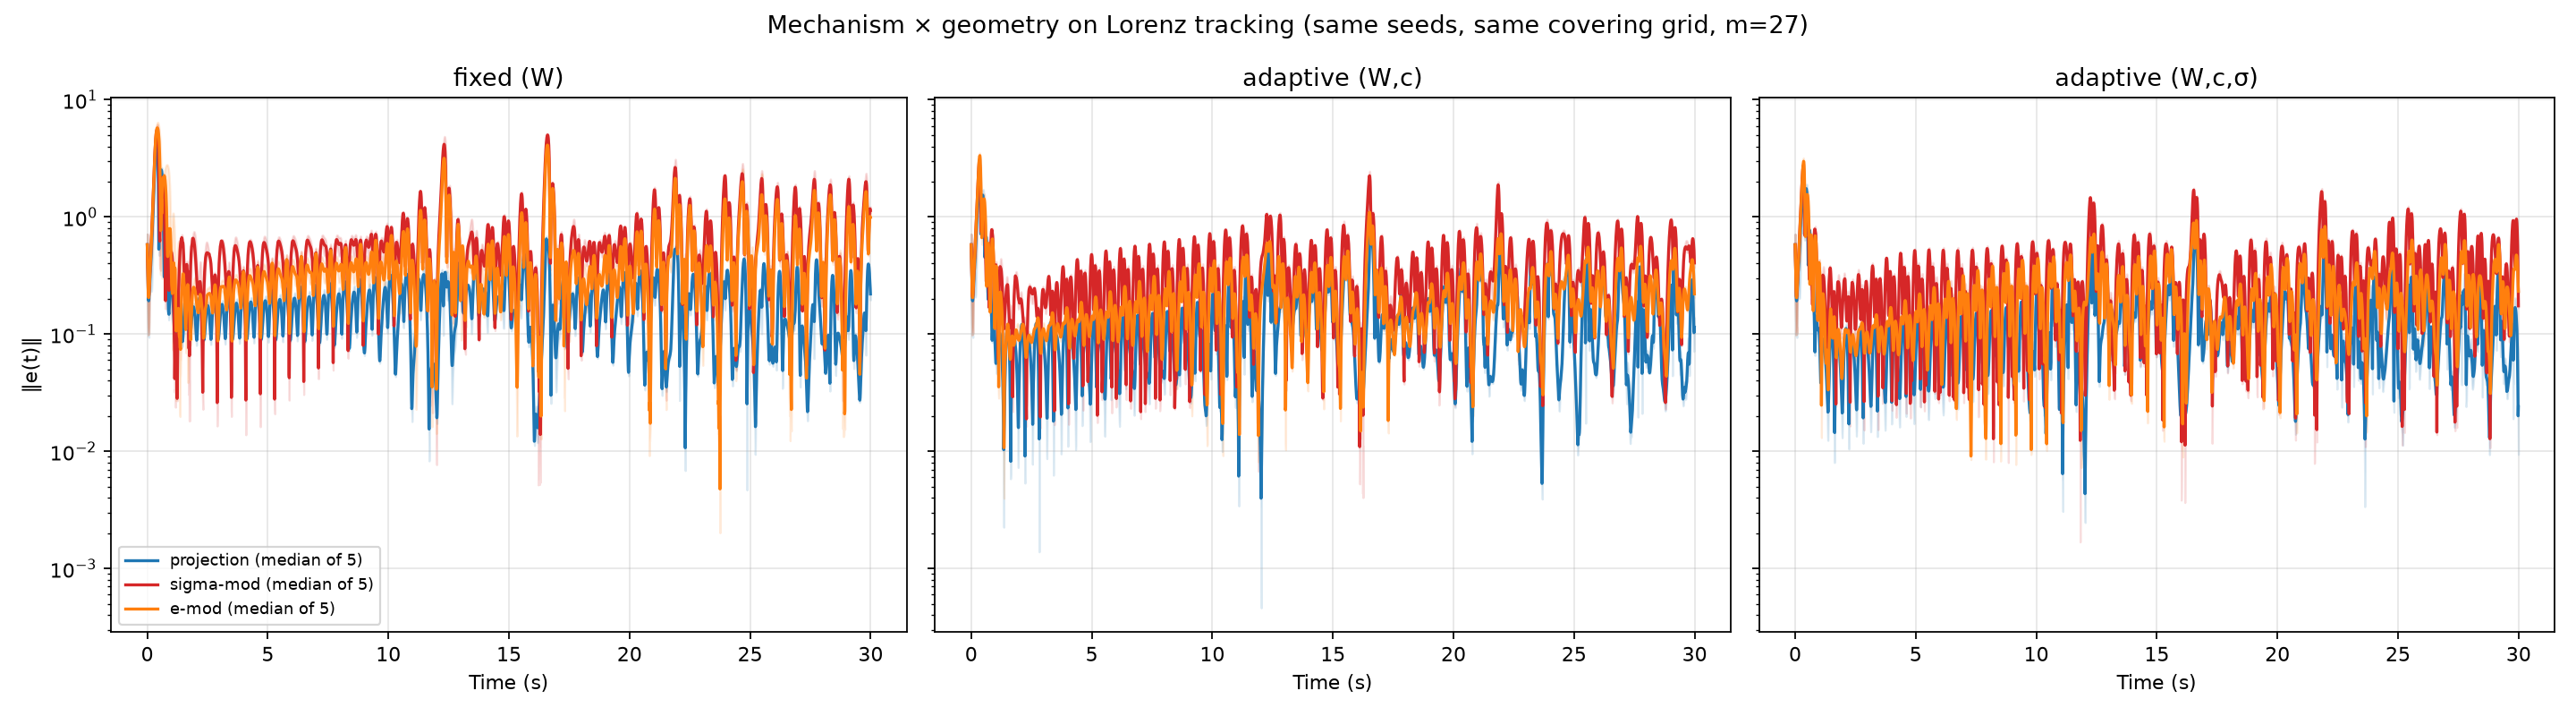
\includegraphics[width=\textwidth]{factorial/figure.png}
\caption[Mechanism $\times$ geometry on Lorenz tracking]{Mechanism $\times$ geometry on Lorenz tracking (same seeds, same covering grid, $m=27$): $\norm{e(t)}$
against time, logarithmic scale, median of the 5 seeds for projection, $\sigma$-modification and $e$-modification;
shaded bands: minimum to maximum over the 5 seeds. Panels: fixed ($W$), adaptive ($W,c$), adaptive ($W,c,\sigma$). Generated by
\code{experiments/exp_bias_factorial.py}.}\label{fig:part1:factorial}
\end{figure}

Projection beats both leaky baselines in every cell, in 5/5 seeds, with paired confidence intervals excluding zero.
Within projection, adaptive centres improve on the fixed grid by $0.0116\pm0.0056$ (5/5 seeds) and adaptive widths
by a further $0.0349\pm0.0026$ (5/5 seeds). So the method's real advantage is the robustness mechanism, with geometry
adaptation a smaller second-order gain --- close to the reverse of the story told by the original headline figure.

\subsection{Kernel-regression baselines}

Table~\ref{tab:part1:complete} is the comparison against kernel-regression baselines from saved single runs, with
nothing excluded (in particular the benchmark $n=3$ and the NTK baseline are included). The proposed method is never
first: it ranks 3/5, 2/5, 3/5 and 2/5 at $n=1,2,3,6$. NTK is first at $n=2$ and $n=6$ (mean steady-state $\norm{e}$
0.0015 and 0.0013, against 0.0372 and 0.0044 for the proposed method), and the sparse GP is first at $n=3$ (3.2729),
where the error of the proposed method is 7.7190. Its genuine edge is cost against the GP baselines: the mean update
time of the proposed method is 0.10, 0.22 and 0.60\,ms per step at $n=1,2,6$ and 4.11\,ms at $n=3$, against
52.92--1888.80\,ms per update for the GP baselines, which update every 50--100 steps. NTK takes 1.59--13.22\,ms per
update; it updates every 50 steps at $n=1$ and every step at $n=2,3,6$ (\code{experiments/sim4_ntk_control.py},
\code{experiments/sim4_ntk_n2.py}, \code{experiments/sim4_ntk_n3.py}, \code{experiments/sim4_ntk_n6.py}), so it is
cheaper than the proposed method only at $n=3$ (2.35 against 4.11\,ms per step). The comparison is not
information-matched: every baseline, here and in the fair re-run below, is trained on noise-free samples of the true
$f(x,t)$, which amounts to measuring the state derivative exactly, whereas the adaptive law uses only the tracking
error $e$. With one run per cell no valid
significance test is available.

\begin{table}[htbp]
\centering\small
\caption[Higher-dimensional comparison, complete]{Higher-dimensional comparison, complete (nothing excluded). Single trajectory per cell; steady state = last
40\% of 30\,s. Step time = mean wall-clock time of the method's update call (GP: per update, every 50--100 steps;
NTK: per update, every 50 steps at $n=1$ and every step at $n=2,3,6$; proposed: per step). No valid significance test
is available (one run per cell). Generated by \code{experiments/plot_comparison_hd_complete.py}; source:
\code{results/comparison_complete_table.md}.}\label{tab:part1:complete}
\begin{tabular}{@{}llrrrcr@{}}
\toprule
benchmark & method & \begin{tabular}[b]{@{}r@{}}mean\\SS $\norm{e}$\end{tabular}
  & \begin{tabular}[b]{@{}r@{}}median\\SS\end{tabular} & \begin{tabular}[b]{@{}r@{}}max\\SS\end{tabular}
  & \begin{tabular}[b]{@{}c@{}}rank\\(mean SS)\end{tabular}
  & \begin{tabular}[b]{@{}r@{}}mean update\\time (ms)\end{tabular}\\
\midrule
$n=1$ (1-D plant, & Proposed (Proj) & 0.2342 & 0.1496 & 1.290 & 3/5 & 0.10\\
\quad Lorenz ref.) & Exact GP & 0.2206 & 0.1415 & 1.016 & 1/5 & 273.78\\
 & Sparse GP & 0.2285 & 0.1914 & 0.874 & 2/5 & 52.92\\
 & Deep GP & 0.3963 & 0.2994 & 1.436 & 4/5 & 94.34\\
 & NTK & 0.4286 & 0.3318 & 1.324 & 5/5 & 13.22\\
\addlinespace
$n=2$ & Proposed (Proj) & 0.0372 & 0.0137 & 0.310 & 2/5 & 0.22\\
\quad (Van der Pol) & Exact GP & 0.0555 & 0.0370 & 0.278 & 3/5 & 498.50\\
 & Sparse GP & 0.1771 & 0.0929 & 0.886 & 5/5 & 150.30\\
 & Deep GP & 0.1758 & 0.1169 & 1.097 & 4/5 & 415.37\\
 & NTK & 0.0015 & 0.0009 & 0.006 & 1/5 & 1.59\\
\addlinespace
$n=3$ & Proposed (Proj) & 7.7190 & 5.7197 & 30.476 & 3/5 & 4.11\\
\quad (Lorenz plant) & Exact GP & 10.2774 & 8.8437 & 34.467 & 5/5 & 1888.80\\
 & Sparse GP & 3.2729 & 2.5099 & 19.176 & 1/5 & 264.64\\
 & Deep GP & 9.5344 & 8.3305 & 33.755 & 4/5 & 802.93\\
 & NTK & 5.7642 & 4.2944 & 18.240 & 2/5 & 2.35\\
\addlinespace
$n=6$ & Proposed (Proj) & 0.0044 & 0.0013 & 0.026 & 2/5 & 0.60\\
\quad (coupled Duffing) & Exact GP & 0.0841 & 0.0695 & 0.279 & 3/5 & 668.01\\
 & Sparse GP & 0.1444 & 0.0872 & 0.670 & 5/5 & 523.83\\
 & Deep GP & 0.0953 & 0.0553 & 0.342 & 4/5 & 1607.48\\
 & NTK & 0.0013 & 0.0010 & 0.004 & 1/5 & 4.75\\
\bottomrule
\end{tabular}
\end{table}

In the original baseline scripts (\code{sim1}--\code{sim3}) the GP baselines held a stale prediction for 50--100 steps,
and the inducing points of the sparse GP lay on a diagonal line over $x\in[-3,3]$ while the reference spans $\pm20$.
The fair re-run at $n=1$ (\code{experiments/kernel_baselines_fair.py}, \code{experiments/run_fair_n1.py},
\code{experiments/plot_fair_n1.py}) uses per-step prediction for all methods, a covering inducing grid and 3 seeds
(Table~\ref{tab:part1:fair}, Figure~\ref{fig:part1:fair}). The mean steady-state $\norm{e}$ is 0.0591 for the exact
GP, 0.1867 for the sparse GP, 0.1978 for the proposed method, 0.3087 for the deep GP and 0.4700 for NTK; the median
online step is 6.309, 1.353, 0.060, 4.461 and 0.212\,ms respectively. Once it is allowed to predict every step, the
exact GP is 3--4$\times$ more accurate than the proposed method (mean steady-state $\norm{e}$ 0.0591 against 0.1978),
and more accurate in every seed (the proposed method has the lower mean in 0/3 seeds). The proposed method is on par
with a fixed-grid sparse GP (the proposed method has the lower mean in 2/3 seeds) at $22.6\times$ lower cost (median
step 0.060\,ms against 1.353\,ms); its step is the cheapest of the five methods. This is the version of the comparison to quote.

\begin{table}[htbp]
\centering\small
\caption[Fair 1-D kernel comparison]{Fair 1-D kernel comparison: per-step prediction for every method, covering inducing grid, seed-level
statistics. Seeds: 3 (different reference and plant initial conditions). Steady state = last 40\% of 30\,s. Step time
= median full online step (prediction + amortised training) after warm-up, same process type, 2 BLAS threads.
Source: \code{results/fair_n1/table.md}.}\label{tab:part1:fair}
\begin{tabular}{@{}lcrrrc@{}}
\toprule
method & \begin{tabular}[b]{@{}c@{}}mean SS $\norm{e}$\\(mean $\pm$ 95\% CI\\over seeds)\end{tabular}
  & \begin{tabular}[b]{@{}r@{}}max SS $\norm{e}$\\(mean)\end{tabular}
  & \begin{tabular}[b]{@{}r@{}}median\\step (ms)\end{tabular}
  & \begin{tabular}[b]{@{}r@{}}mean\\step (ms)\end{tabular}
  & \begin{tabular}[b]{@{}c@{}}seeds where\\proposed has\\lower mean SS\end{tabular}\\
\midrule
Proposed (Proj) & $0.1978\pm0.0503$ & 1.147 & 0.060 & 0.069 & ---\\
Exact GP & $0.0591\pm0.0061$ & 0.780 & 6.309 & 13.936 & 0/3\\
Sparse GP ($9\times3$ grid) & $0.1867\pm0.0210$ & 0.699 & 1.353 & 2.732 & 2/3\\
Deep GP & $0.3087\pm0.1121$ & 1.262 & 4.461 & 5.495 & 2/3\\
NTK & $0.4700\pm0.0250$ & 1.438 & 0.212 & 0.503 & 3/3\\
\bottomrule
\end{tabular}
\end{table}

\begin{figure}[htbp]
\centering
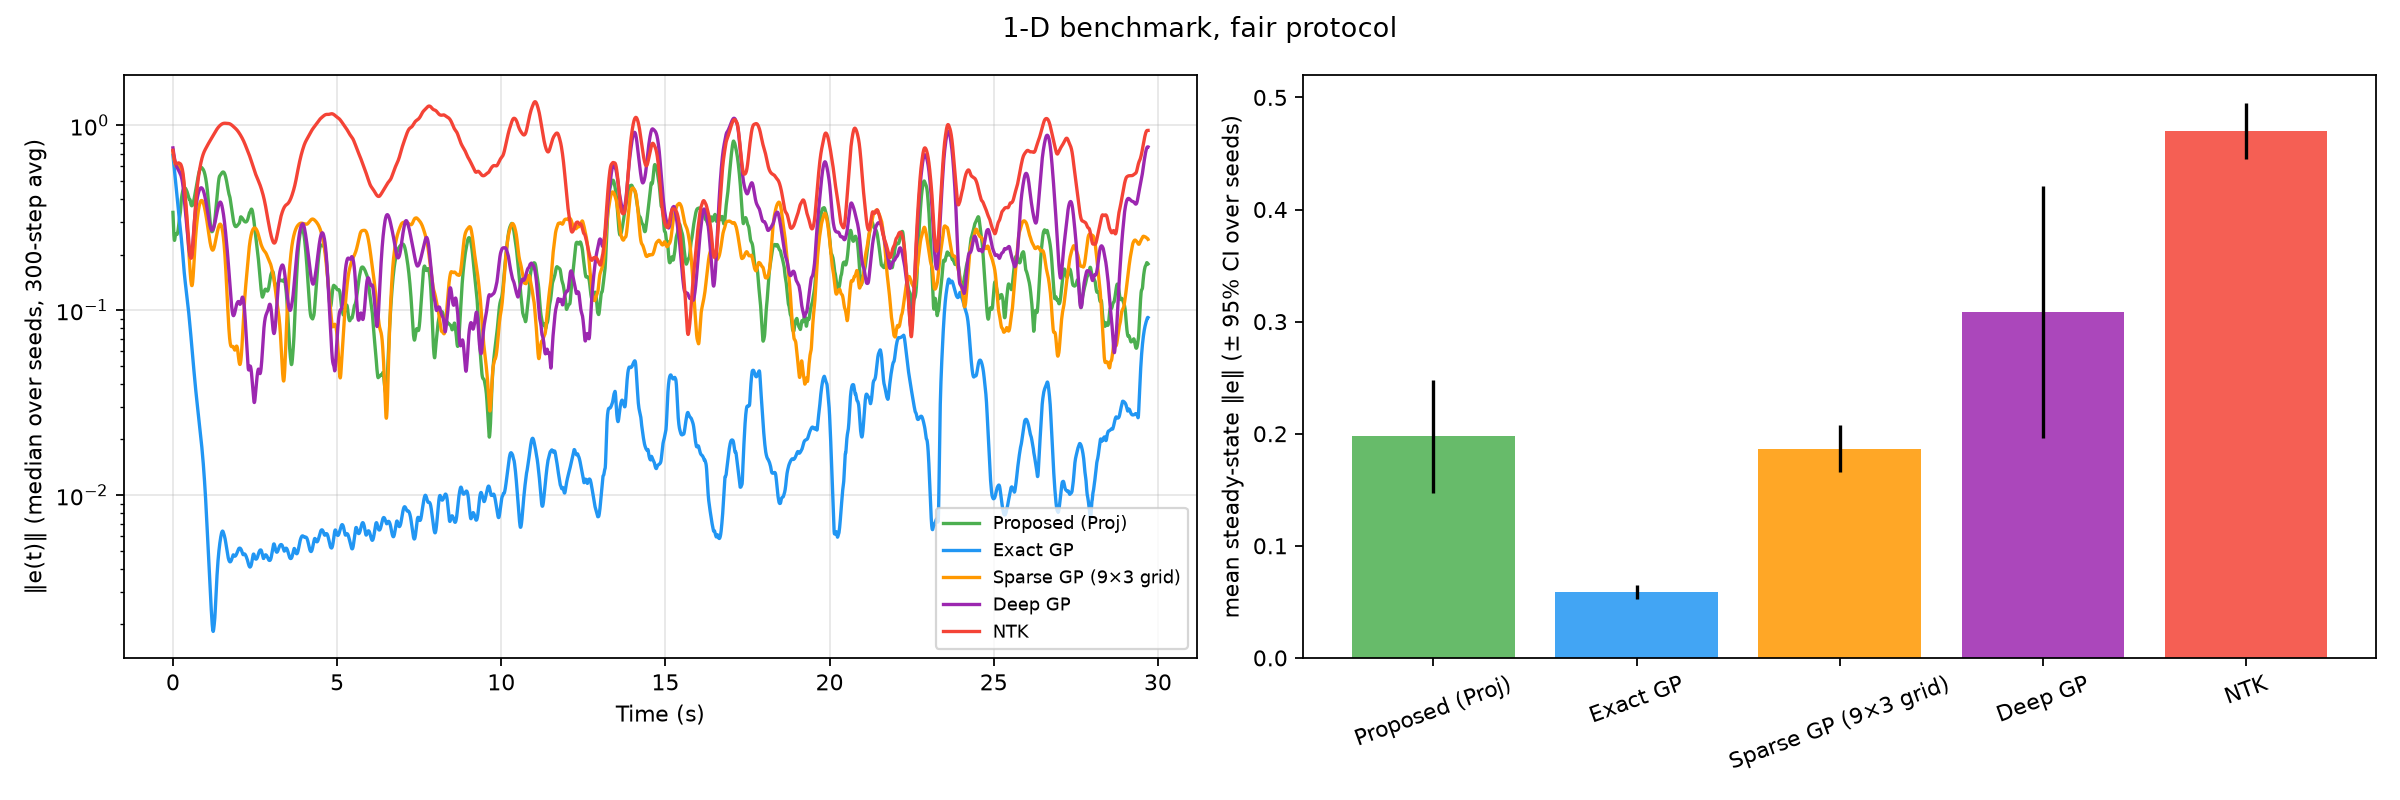
\includegraphics[width=\textwidth]{fair_n1/figure.png}
\caption[1-D benchmark, fair protocol]{1-D benchmark, fair protocol. Left: $\norm{e(t)}$ (median over seeds, 300-step average), logarithmic scale,
for the proposed method (Proj), the exact GP, the sparse GP ($9\times3$ grid), the deep GP and NTK. Right: mean
steady-state $\norm{e}$ ($\pm$ 95\% CI over seeds). Generated by \code{experiments/plot_fair_n1.py}; numbers in
Table~\ref{tab:part1:fair}.}\label{fig:part1:fair}
\end{figure}

\subsection{The bound against data}

\paragraph{Oracle bound study.} The oracle experiment (\code{experiments/exp_oracle_ruub.py}) uses a plant that is
exactly representable with constant $\theta^*$ ($m=8$, $n=2$), so every constant of Theorem~1 is computable; with $\theta^*$ constant,
$C_\Omega=0$ and $R_{\mathrm{UUB}}=D_{\max}/k_e$, reported as $D_{\mathrm{theory}}/k_e$ with $D_{\max}$ from Lemma~2.
The ``full-state bound'' is $\sqrt{R_{\mathrm{UUB}}^2+2V_{\max,\Theta}}$ of Theorem~1(ii), and $D_{\mathrm{meas}}$ is
the measured $\sup_{t\in[10,30]}\norm{d(t)}$ over the evaluation window. Table~\ref{tab:part1:oracle} and
Figure~\ref{fig:part1:oracle} cover $k_e\in\{2,5,10,20\}$ and four learning-rate scales, 3 seeds each. The Lyapunov
identity of Lemma~3 holds to $3.55\times10^{-15}$ (maximal $\abs{\dot V-(-k_e\norm{e}^2+e^\T d+\mathrm{cross})}$),
property (P) is never violated, the hard bounds held, and the RMS bound of Theorem~1(iii) with the measured
disturbance holds in 48/48 runs and tracks $1/k_e$. The a-priori $R_{\mathrm{UUB}}$ is 26.1--261.1 against observed
RMS errors of 0.0087--0.0908; the ratio of the a-priori bound to the observed RMS error ranges from $915\times$ to
$10954\times$.

\begin{table}[htbp]
\centering\footnotesize\setlength{\tabcolsep}{4pt}
\caption[Oracle $R_{\mathrm{UUB}}$ study]{Oracle $R_{\mathrm{UUB}}$ study (exactly representable plant, constant $\theta^*$, $m=8$, $n=2$). Window
$[10,30]$\,s; mean over 3 seeds. All bounds in the same units as $\norm{e}$. ``P viol'' = samples with
$\mathrm{cross}>0$ (must be 0); ``inside'' = hard bounds held. RMS bound (measured disturbance) satisfied in all 48
runs: True. Maximal identity error $\abs{\dot V-(-k_e\norm{e}^2+e^\T d+\mathrm{cross})}$: $3.55\times10^{-15}$.
Source: \code{results/oracle_ruub/table.md}.}\label{tab:part1:oracle}
\begin{tabular}{@{}rrrrrrrrrcc@{}}
\toprule
$k_e$ & \begin{tabular}[b]{@{}r@{}}$\Gamma$\\scale\end{tabular}
  & \begin{tabular}[b]{@{}r@{}}RMS\\$\norm{e}$\end{tabular}
  & \begin{tabular}[b]{@{}r@{}}max SS\\$\norm{e}$\end{tabular}
  & \begin{tabular}[b]{@{}r@{}}RMS bound\\($D_{\mathrm{meas}}$,\\finite window)\end{tabular}
  & $D_{\mathrm{meas}}/k_e$ & $D_{\mathrm{theory}}/k_e$
  & \begin{tabular}[b]{@{}r@{}}full-state\\bound\end{tabular}
  & \begin{tabular}[b]{@{}r@{}}ratio\\theory/RMS\end{tabular}
  & \begin{tabular}[b]{@{}c@{}}P\\viol\end{tabular} & inside\\
\midrule
2 & 0.5 & 0.0908 & 0.1704 & 0.6791 & 0.5435 & 261.1 & 261.9 & 2875$\times$ & 0 & True\\
2 & 1 & 0.0616 & 0.1215 & 0.6801 & 0.6123 & 261.1 & 261.5 & 4239$\times$ & 0 & True\\
2 & 2 & 0.0383 & 0.0796 & 0.7139 & 0.6808 & 261.1 & 261.3 & 6824$\times$ & 0 & True\\
2 & 5 & 0.0238 & 0.0476 & 1.1766 & 1.1649 & 261.1 & 261.2 & 10954$\times$ & 0 & True\\
\addlinespace
5 & 0.5 & 0.0533 & 0.1054 & 0.3170 & 0.1979 & 104.4 & 106.4 & 1958$\times$ & 0 & True\\
5 & 1 & 0.0392 & 0.0708 & 0.2793 & 0.2123 & 104.4 & 105.4 & 2664$\times$ & 0 & True\\
5 & 2 & 0.0270 & 0.0539 & 0.2601 & 0.2240 & 104.4 & 104.9 & 3866$\times$ & 0 & True\\
5 & 5 & 0.0157 & 0.0329 & 0.2925 & 0.2780 & 104.4 & 104.6 & 6662$\times$ & 0 & True\\
\addlinespace
10 & 0.5 & 0.0398 & 0.0793 & 0.1970 & 0.0981 & 52.2 & 56.1 & 1313$\times$ & 0 & True\\
10 & 1 & 0.0266 & 0.0519 & 0.1596 & 0.1003 & 52.2 & 54.2 & 1965$\times$ & 0 & True\\
10 & 2 & 0.0194 & 0.0369 & 0.1395 & 0.1057 & 52.2 & 53.2 & 2688$\times$ & 0 & True\\
10 & 5 & 0.0117 & 0.0240 & 0.1335 & 0.1188 & 52.2 & 52.6 & 4466$\times$ & 0 & True\\
\addlinespace
20 & 0.5 & 0.0285 & 0.0522 & 0.1290 & 0.0501 & 26.1 & 33.2 & 915$\times$ & 0 & True\\
20 & 1 & 0.0197 & 0.0389 & 0.0987 & 0.0494 & 26.1 & 29.9 & 1328$\times$ & 0 & True\\
20 & 2 & 0.0132 & 0.0260 & 0.0799 & 0.0503 & 26.1 & 28.0 & 1971$\times$ & 0 & True\\
20 & 5 & 0.0087 & 0.0168 & 0.0676 & 0.0534 & 26.1 & 26.9 & 3011$\times$ & 0 & True\\
\bottomrule
\end{tabular}
\end{table}

\begin{figure}[htbp]
\centering
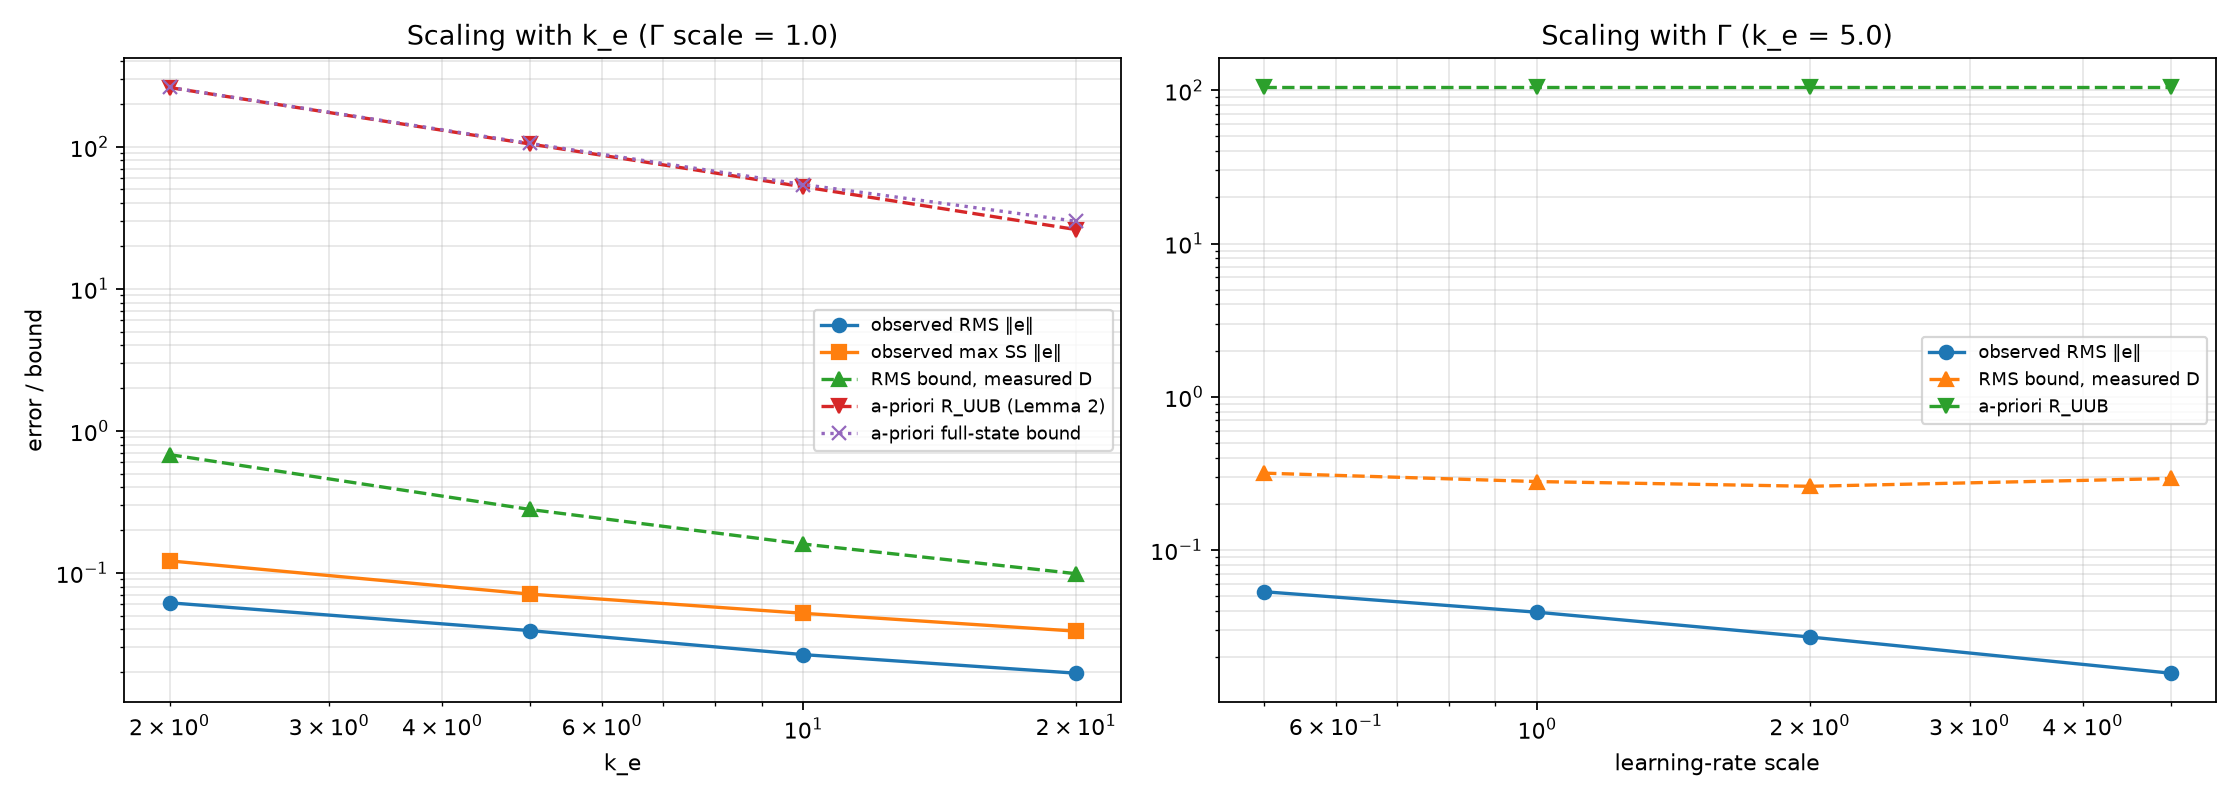
\includegraphics[width=\textwidth]{oracle_ruub/figure.png}
\caption[Oracle bound study]{Oracle bound study, logarithmic axes. Left: scaling with $k_e$ at learning-rate scale 1.0 --- observed RMS
$\norm{e}$, observed maximal steady-state $\norm{e}$, the RMS bound with the measured disturbance, the a-priori
$R_{\mathrm{UUB}}$ (Lemma~2) and the a-priori full-state bound. Right: scaling with the learning-rate scale at $k_e=5$
--- observed RMS $\norm{e}$, the RMS bound with the measured disturbance and the a-priori $R_{\mathrm{UUB}}$. Generated
by \code{experiments/exp_oracle_ruub.py}; numbers in Table~\ref{tab:part1:oracle}.}\label{fig:part1:oracle}
\end{figure}

\begin{table}[htbp]
\centering\small
\caption[Monte Carlo over random initial conditions]{Monte Carlo over random initial conditions (Van der Pol, $m=16$, $k_e=5.0$, 200 trials). Source:
\code{results/monte_carlo_honest/summary.md}.}\label{tab:part1:mc}
\begin{tabularx}{\textwidth}{@{}Yl@{}}
\toprule
check & result\\
\midrule
all trajectories finite & 200/200\\
hard parameter bounds held at every recorded step & 200/200\\
a-posteriori ISS bound
  $\norm{e(t)}\le\mathrm{e}^{-k_e(t-T_1)}\norm{e(T_1)}+\sup\norm{f-\fhat}/k_e$ held & 200/200 (max ratio 0.979)\\
steady-state max $\norm{e}$ (last 25\%): median / 95th pct / max & 0.0568 / 0.0938 / 0.1075\\
steady-state mean $\norm{e}$: median / 95th pct / max & 0.0302 / 0.0484 / 0.0593\\
$\sup\norm{f-\fhat}$ in steady state / $k_e$: median / max & 0.0627 / 0.1475\\
transient max $\norm{e}$: max over trials & 4.903\\
\bottomrule
\end{tabularx}
\end{table}

\paragraph{Monte Carlo over initial conditions.} On a plant that is not exactly representable only exactly checkable
statements are tested (\code{experiments/exp_monte_carlo_honest.py}, Table~\ref{tab:part1:mc}): all 200 trajectories
are finite, the hard parameter bounds held at every recorded step in 200/200 trials, and the a-posteriori ISS bound
held in 200/200 trials (maximal ratio 0.979). No a-priori $R_{\mathrm{UUB}}$ threshold is drawn: $D_{\max}$ and
$C_\Omega$ are not computable for this plant (the threshold 0.5 of the original figure was an arbitrary constant, not a
calculated bound).

\subsection{Summary}

\begin{itemize}
\item On identical geometry, projection beats $\sigma$- and $e$-modification in every cell and in every seed (5/5),
  with paired confidence intervals excluding zero.
\item Adaptive geometry is a smaller but consistent gain: $0.0116$ for adaptive centres and a further $0.0349$ for
  adaptive widths in mean steady-state $\norm{e}$, 5/5 seeds each.
\item Against kernel-regression baselines the proposed method is never the most accurate. Its edge is cost against the
  GP baselines (NTK is cheaper only at $n=3$), and in the fair re-run at $n=1$ it has the cheapest step of the five
  methods.
\item In the fair re-run at $n=1$ the exact GP is 3--4$\times$ more accurate than the proposed method.
\item In the oracle study the a-priori bound exceeds the observed RMS error by factors of $915$ to $10954$, while the
  RMS bound with the measured disturbance holds in 48/48 runs.
\end{itemize}


\clearpage
\part{Transport adaptive control}
% PARADIGM.md section 1 (Setting).  File id: setting.
\section{Setting}\label{sec:setting}

\paragraph{Plant, reference, control, error.}
\[
  \dot x = f(x,t) + u,\qquad e = x - x_m(t),\qquad u = \dot x_m - k_e e - \fhat(x).
\]

\paragraph{Lifted parameter.}
$\vartheta = (a,c,s)\in\R^n\times\R^n\times\R_{>0}$, and $p := 2n+1$. The feature is
${\Phi(x;\vartheta) := a\,\varphi(x;c,s)}\in\R^n$, where $\varphi(x;c,s) = \exp\bigl(-\norm{x-c}^2/(2s^2)\bigr)$.

\paragraph{Network as a measure.}
\[
  \fhat(x) = \frac1m\sum_{i=1}^m \Phi(x;\vartheta_i) = \int\Phi(x;\vartheta)\dd\mu(\vartheta),
  \qquad \mu := \frac1m\sum_{i=1}^m\delta_{\vartheta_i}.
\]
The map $\mu\mapsto\fhat$ is linear.

\paragraph{Metric.}
$G = \operatorname{diag}(g_a I_n, g_c I_n, g_s)\succ 0$ is the gain matrix. Distances are measured in
$\norm{v}_{\Ginv}^2 = v^\T\Ginv v$, and $\lambda_G := \lambda_{\max}(G)$.

\paragraph{Admissible box and projection.}
\begin{itemize}
  \item \textbf{The box.}
    $\ThK := \{\norm{a}\le a_{\max}\}\times\{\norm{c}\le c_{\max}\}\times[s_{\min},s_{\max}]$.
  \item \textbf{Layer and inner set.} $\varepsilon_K$ is the width of the boundary layer. Shrinking each bound of
    $\ThK$ by $\varepsilon_K$ gives the inner set $\ThKe$, with interior $\operatorname{int}\ThKe$.
  \item \textbf{The operator.} $\Proj(\vartheta,y)$ is the per-particle, factor-wise projection (implemented in
    \code{src/core/projection.py} in the accompanying repository). It uses Pomet--Praly norm-ball
    operators~\cite{pp1992} for $a$ and $c$, with a quadratic ramp $h\in[0,1]$ (defined in Section~\ref{sec:p1-algorithm}), and a box operator for $s$, with a
    linear ramp.
  \item \textbf{Regularity.} The operator is locally Lipschitz in $(\vartheta,y)$. The norm-ball factors are $C^1$ at
    the inner edge of their layers. The box factor, and every factor at the outer edge, is only Lipschitz. The proofs
    use only Lipschitz continuity and ramp values in $[0,1]$.
\end{itemize}

\paragraph{Property (P).}
For $\vartheta\in\ThK$, $\vartheta'\in\ThKe$ and all $y$,
\begin{equation}\label{eq:setting:P}
  \ip{\vartheta-\vartheta'}{\Ginv\Proj(\vartheta,Gy)} \le \ip{\vartheta-\vartheta'}{y}.
  \tag{P}
\end{equation}
On $\partial\ThK$ the projected velocity has no outward component, so $\ThK$ is forward invariant (Nagumo;
Pomet--Praly 1992~\cite{pp1992}).

\begin{thm}{Lemma}{P.1}[$\Proj$ is non-expansive]
For every $\vartheta = (a,c,s)\in\ThK$ and $y = (y_a,y_c,y_s)$,
\[
  \norm{\Proj(\vartheta,Gy)}_{\Ginv}^2
  = \norm{y}_G^2 - \sum_{b\in\{a,c,s\}} h_b(2-h_b)\,\frac{\bigl[(n_b^\T G_b y_b)_+\bigr]^2}{n_b^\T G_b n_b}
  \;\le\; \norm{y}_G^2 .
\]
The terms are as follows.
\begin{itemize}
  \item For the balls, $n_a = a$ and $n_c = c$, with the quadratic ramps $h_a = h(\norm{a};a_{\max},\varepsilon_K)$ and
    $h_c = h(\norm{c};c_{\max},\varepsilon_K)$.
  \item For $s < s_{\min}+\varepsilon_K$, $n_s = -1$ and $h_s = 1-\clip\bigl((s-s_{\min})/\varepsilon_K,0,1\bigr)$.
  \item For $s > s_{\max}-\varepsilon_K$, $n_s = +1$ and $h_s = 1-\clip\bigl((s_{\max}-s)/\varepsilon_K,0,1\bigr)$.
  \item Otherwise $h_s = 0$.
\end{itemize}
\end{thm}

\begin{proof}
$G$ is block-diagonal, so both squared norms split over the blocks. On an active ball block,
$\operatorname{Proj}_b = G_b q_b$ with $q_b = y_b - h_b n_b\,(n_b^\T G_b y_b)/(n_b^\T G_b n_b)$. Expanding
$q_b^\T G_b q_b$ gives the subtracted term. On an inactive block ($h_b = 0$ or $n_b^\T G_b y_b\le 0$),
$\operatorname{Proj}_b = G_b y_b$. The $s$-block is the one-dimensional case. Finally $h_b\in[0,1]$, so
$h_b(2-h_b)\in[0,1]$.
\end{proof}
\checkedby{\code{tests/test_transport.py}: \code{test_lemma_P1_projection_is_nonexpansive_and_tight_velocity_bound}.}

\paragraph{Potential.}
$g_t(\vartheta) := e(t)^\T\Phi(x(t);\vartheta)$, and $F_t(\mu) := -\int g_t\dd\mu = -e(t)^\T\fhat(x(t))$.

\paragraph{Adaptive law (the algorithm).}
\begin{equation}\label{eq:setting:L}
  \dot\vartheta_i = \Proj\bigl(\vartheta_i,\, G\nabla_\vartheta g_t(\vartheta_i)\bigr),\qquad i = 1,\dots,m.
  \tag{L}
\end{equation}

\paragraph{Ideal measure.}
For $j = 1,\dots,m$, $\vartheta^*_j(t)\in\ThKe$ is $C^1$ in $t$, and
$\mu^*_t := \frac1m\sum_j\delta_{\vartheta^*_j(t)}$. Write
$\varepsilon(x,t) := f(x,t) - \int\Phi(x;\cdot)\dd\mu^*_t$, with $\norm{\varepsilon}\le\varepsilon_{\max}$ on the
operating set $X$, and set
\[
  V_*(t) := \Bigl(\frac1m\sum_j\norm{\dot\vartheta^*_j}_{\Ginv}^2\Bigr)^{1/2},\qquad V_* := \sup_t V_*(t).
\]
The proofs never use optimality of $\mu^*$. It is an analytic device, and any admissible $C^1$ curve may be used.

\paragraph{Optimal-transport distance.}
For uniform atomic $\mu = \frac1m\sum\delta_{\vartheta_i}$ and $\nu = \frac1m\sum\delta_{\vartheta'_j}$,
\[
  W(\mu,\nu)^2 := \min_{\pi\in S_m}\frac1m\sum_i\norm{\vartheta_i-\vartheta'_{\pi(i)}}_{\Ginv}^2 .
\]
This is the Kantorovich $2$-Wasserstein distance with ground cost $\norm{\cdot}_{\Ginv}^2$. For equal masses the
optimum is attained at a permutation (Birkhoff). It is computed by linear assignment in $O(m^3)$. For general measures
on $\ThK$, $W$ denotes the same Kantorovich distance.

\paragraph{Label-free Lyapunov function.}
\begin{align*}
  \VOT(t) &:= \tfrac12\norm{e(t)}^2 + \tfrac12 W(\mu_t,\mu^*_t)^2 = \min_\pi V_\pi(t),\\
  V_\pi &:= \tfrac12\norm{e}^2 + \frac1{2m}\sum_i\norm{\vartheta_i-\vartheta^*_{\pi(i)}}_{\Ginv}^2 .
\end{align*}

\paragraph{Standing hypotheses (S).}
\begin{enumerate}[label=(S\arabic*),start=0]
  \item $k_e>0$; $G = \operatorname{diag}(g_a I_n, g_c I_n, g_s)\succ 0$; $s_{\min}>0$; and
    $0<\varepsilon_K<\min\{a_{\max},c_{\max},(s_{\max}-s_{\min})/2\}$ (\code{src/core/projection.py} enforces the
    last condition).
  \item $f$ is continuous in $(x,t)$ and locally Lipschitz in $x$, uniformly in $t$ on bounded time intervals.
  \item $x_m\in C^1$, and $x_m$ and $\dot x_m$ are bounded.
  \item $\vartheta_i(0)\in\ThK$.
  \item The $\vartheta^*_j$ are $C^1$ with values in $\ThKe$, and $V_*<\infty$.
  \item $x(t)\in X$ on the interval considered. For bounded $f$, take
    $X := \bigcup_t\{x : \norm{x-x_m(t)}\le r(F)\}$ with $F = \sup\norm{f}$ (Theorem D(b)). Then $\varepsilon_{\max}$
    is the supremum over this $X$, and it depends on $\norm{e(0)}$.
\end{enumerate}
Under (S0)--(S3) the right-hand side of (L) is continuous in $t$ and locally Lipschitz in $(x,\vartheta)$. Solutions
are classical ($C^1$) and unique on their maximal interval. Under (S4) as well, each $V_\pi$ is $C^1$.

\paragraph{Notation.}
\begin{itemize}
  \item Times are written $t_0\le t_1$ (or $T_1<T_2$), and $r$ is the integration variable in time.
  \item $\RMS_{[T_1,T_2]}\norm{e} := \Bigl((T_2-T_1)^{-1}\int_{T_1}^{T_2}\norm{e}^2\dd r\Bigr)^{1/2}$.
\end{itemize}

\paragraph{Constants of the Gaussian.} Closed forms (\code{gaussian_constants} in \code{src/core/transport.py} of the
accompanying repository). With $u := \norm{x-c}^2/s^2$ and
$\varphi = e^{-u/2}$, on $s\ge s_{\min}$:
\begin{gather*}
  \norm{\nabla_c\varphi}\le J_c := e^{-1/2}/s_{\min},\qquad
  \abs{\partial_s\varphi}\le J_s := 2e^{-1}/s_{\min},\qquad
  J := (J_c^2+J_s^2)^{1/2},\\
  \norm{\nabla^2_{(c,s)}\varphi}\le H_\varphi := \bigl(\max(h_{cc},h_{ss}) + h_{cs}\bigr)/s_{\min}^2,\\
  h_{cc} = 1,\qquad h_{ss} = 2e^{-1/2},\qquad
  h_{cs} = \sqrt u\,e^{-u/2}\abs{u-2}\ \text{ evaluated at } u = (5-\sqrt{17})/2 .
\end{gather*}
$J$ and $H_\varphi$ are upper bounds. The true supremum of $\norm{\nabla_{(c,s)}\varphi}$ is about $0.92/s_{\min}$,
and that of $\norm{\nabla^2_{(c,s)}\varphi}$ is about $1.57/s_{\min}^2$. The Hessian of the lifted potential is the
block matrix
\[
  \begin{pmatrix} 0 & u\,\nabla\varphi^\T\\[2pt] \nabla\varphi\,u^\T & (u^\T a)\,\nabla^2\varphi\end{pmatrix}.
\]
Hence
\begin{equation}\label{eq:setting:HK}
  \sup_{x\in\R^n,\ \vartheta\in\ThK,\ \norm{u}=1}\norm{\nabla^2_\vartheta\bigl(u^\T\Phi(x;\vartheta)\bigr)}
  \le H_K := J + a_{\max}H_\varphi,\qquad K := \tfrac12 H_K.
  \tag{1}
\end{equation}
A brute-force numerical check over the full lifted Hessian gives $\sup\approx 0.76\,H_K$.

% PARADIGM.md section 2 (Theorem A).  File id: thmA.
\section{Theorem A: identification}\label{sec:thmA}

\begin{thm}{Theorem}{A}
Assume \textup{(S0)}.
\begin{enumerate}[label=(\roman*)]
  \item Assume scalar classical gains $\Gamma_W = \gamma_W I$, $\Gamma_c = \gamma_c I$ and
    $\Gamma_\sigma = \gamma_\sigma I$, and use the dictionary $W_i = a_i/m$, $\gamma_W = g_a/m$, $\gamma_c = m g_c$,
    $\gamma_\sigma = m g_s$.
    \begin{itemize}
      \item The \emph{raw} \textup{(}unprojected\textup{)} rates of \textup{(L)} and of the classical law of
        Section~\ref{sec:p1-algorithm} coincide.
      \item The \emph{projected} rates coincide when the classical joint projections are replaced by per-kernel
        ones. The classical law projects $W$ onto one Frobenius ball and $\operatorname{vec}(c)$ onto one Euclidean
        ball. The per-kernel version projects:
        \begin{itemize}
          \item $W_i$ onto $\norm{W_i}\le a_{\max}/m$, with layer $\varepsilon_K/m$;
          \item $c_i$ onto $\norm{c_i}\le c_{\max}$, with layer $\varepsilon_K$;
          \item $\sigma_i$ onto $[s_{\min},s_{\max}]$, with layer $\varepsilon_K$.
        \end{itemize}
      \item For $m\ge 2$, no joint ball, of any radius $W_{\max}$ and layer $\varepsilon_W$, reproduces the
        per-kernel field. For $m = 1$ the two coincide, with $W_{\max} = a_{\max}$ and layer $\varepsilon_K$.
    \end{itemize}
  \item Fix a closed-loop trajectory $(x(\cdot),e(\cdot))$. Then:
    \begin{itemize}
      \item The field $v_t(\vartheta) := \Proj(\vartheta, G\nabla g_t(\vartheta))$ is Lipschitz in $\vartheta$ on
        $\ThK$, and $\ThK$ is forward invariant.
      \item For every $\mu_0\in\Prob(\ThK)$, $\mu_t := (X_t)_\#\mu_0$ is a distributional solution of
        $\partial_t\mu + \nabla\cdot(\mu v_t) = 0$.
      \item On $\operatorname{int}\ThKe$, $v_t = -G\nabla(\delta F_t/\delta\mu)$. So at frozen time, $\mu_t$ is the
        Wasserstein gradient flow \textup{(}metric $\Ginv$\textup{)} of the linear functional $F_t$, and
        \textup{(L)} is its particle form.
      \item $F_t$ is generated by the closed loop, so the coupled system is the one studied in Theorem D.
    \end{itemize}
  \item \textbf{Dictionary}, all in the $\Ginv$ metric:

    \smallskip
    {\normalfont\small
    \begin{tabularx}{\linewidth}{@{}>{\hsize=0.8\hsize\raggedright\arraybackslash}X
                                    >{\hsize=1.2\hsize\raggedright\arraybackslash}X@{}}
      \toprule
      classical device & measure-level object\\
      \midrule
      projection onto $\ThK$ &
      A velocity-level (Pomet--Praly) regularisation of the support constraint $\mu_t\in\Prob(\ThK)$. For
      $\varepsilon_K>0$ it is not the gradient flow of any functional of $\mu$. Formally, as $\varepsilon_K\to 0$,
      the field tends to the $\Ginv$-projection of $G\nabla g_t$ onto the tangent cone of $\ThK$, which is the
      velocity of the $\WG$-gradient flow of $F_t + \iota_{\Prob(\ThK)}$ (\cite[Prop.~3.1]{R46} for the exact $W_2$
      projection).\\
      \addlinespace
      $\sigma$-modification in the $\Ginv$ metric (leak outside the gain,
      $\dot\vartheta = G\nabla g - \sigma(\vartheta-\vartheta^0)$, as in $\Lsig$ and Theorem H) &
      the potential energy $(\sigma/2)\int\norm{\vartheta-\vartheta^0}_{\Ginv}^2\dd\mu$, which is geodesically
      $\sigma$-convex\\
      \addlinespace
      classical $\sigma$-modification $\Gamma(y-\sigma\theta)$ (leak inside the gain;
      \code{src/baselines/sigma_mod.py} implements its $W$-block, with $c$ and $\sigma$ frozen) &
      For the full-vector leak, under (i), the object is
      $(\sigma/2)\int(\vartheta-\vartheta^0)^\T D(\vartheta-\vartheta^0)\dd\mu$ with
      $D = \operatorname{diag}(I_n/m, mI_n, m)$. In the $\Ginv$ metric it is $\lambda$-convex with
      $\lambda = \sigma\cdot\min(g_a/m, mg_c, mg_s)$, which depends on $m$. For the $W$-block alone it is
      $(\sigma/2)\int(a-a^0)^\T(I_n/m)(a-a^0)\dd\mu$.\\
      \addlinespace
      $\sigma$-modification toward a labelled $(\vartheta^0_i)$ &
      not a functional of $\mu$; it is a functional on the labelled lift $\R^{mp}$\\
      \addlinespace
      OT $\sigma$-modification (Theorem C) &
      $(\sigma/2)W(\mu,\mu^0)^2$. For atomic $\mu$ with a unique optimal assignment, its $W$-gradient at atom $i$ is
      $\sigma(\vartheta_i-\vartheta^0_{\tau(i)})$. At ties, $\Lsig$ uses a measurable selection from the
      superdifferential $\{\sigma(\vartheta_i-\vartheta^0_{\tau(i)}) : \tau\text{ optimal}\}$.\\
      \addlinespace
      $e$-modification & the same functionals with coefficient $\sigma\norm{e}$\\
      \addlinespace
      parameter dither (Theorem H) & the entropy $\tau\int\mu\log\mu$\\
      \bottomrule
    \end{tabularx}}
\end{enumerate}
\end{thm}
\status{Proved and checked. Novelty (literature audit): interpretive; ingredients known
\cite{R29}, \cite{R41}, \cite{R46}, \cite{R25}.}
\checkedby{\code{tests/test_transport.py}: \code{test_identification_with_classical_law} (raw rates in (i));\newline
\code{test_identification_projected_rates_per_kernel} (projected rates and the only-if construction in (i)).}

\begin{proof}
\textbf{(i)} \textbf{Gain map.} We have $\nabla_a g = \varphi e$, $\nabla_c g = (a^\T e)\nabla_c\varphi$ and
$\partial_s g = (a^\T e)\partial_s\varphi$. Matching these with the classical rates gives the gain map.

\textbf{Scaling identity.}
$(1/m)\operatorname{Proj}_{r,\varepsilon}(a,y) = \operatorname{Proj}_{r/m,\varepsilon/m}(a/m, y/m)$. Three facts give
it:
\begin{itemize}
  \item $h_{r/m,\varepsilon/m}(\norm{a}/m) = h_{r,\varepsilon}(\norm{a})$;
  \item the direction $a(a^\T y)/\norm{a}^2$ is homogeneous of degree $0$ in $a$ and of degree $1$ in $y$;
  \item the activation $a^\T y>0$ is invariant under scaling.
\end{itemize}
If the layer is not rescaled, the ramps differ.

\emph{Only if \textup{(}$m\ge 2$\textup{)}.} Let $r_{\mathrm{in}} := (a_{\max}-\varepsilon_K)/m$, and let the joint
ball have radius $W_{\max}$, layer $\varepsilon_W$ and $\rho := W_{\max}-\varepsilon_W$. In both cases below the
driving term points outward.
\begin{itemize}
  \item If $\rho<\sqrt2\,r_{\mathrm{in}}$, take two rows of equal norm $r$ with
    $\sqrt2\,r\in\bigl(\rho,\min(\sqrt2\,r_{\mathrm{in}},W_{\max})\bigr]$, parallel to $e$. The per-kernel field is
    inactive and the joint field is active.
  \item If $\rho\ge\sqrt2\,r_{\mathrm{in}}$, take one row with norm in
    $\bigl(r_{\mathrm{in}},\min(a_{\max}/m,\rho)\bigr)$ and the others zero. The per-kernel field is active and the
    joint field is inactive.
\end{itemize}
The same argument applies to $\operatorname{vec}(c)$. For $m = 1$ the two operators coincide.

The test \code{test_identification_projected_rates_per_kernel} checks three things: the identity with active projections; that the layer must be
rescaled; and the only-if construction against \code{ProjectionOperator.project_matrix} on five joint balls. Four are
active against an inactive per-kernel field, and one is inactive against an active per-kernel field.

\textbf{(ii)} $\Proj$ is Lipschitz in $\vartheta$. The ramp vanishes for
$\norm{\vartheta}\le\theta_{\max}-\varepsilon_K$, so the direction $\vartheta/\norm{\vartheta}$ is evaluated only away
from $0$. Also, $\nabla g_t$ is $C^1$ on $s\ge s_{\min}$.
\begin{itemize}
  \item \textbf{Invariance.} Forward invariance follows from Nagumo's theorem, since
    $n_b^\T\operatorname{Proj}_b\le 0$ on the boundary, with the outward normals $n_b$ of Lemma P.1.
  \item \textbf{Continuity equation.} The push-forward of $\mu_0$ by a Lipschitz flow solves the continuity equation
    (Golse~\cite{R82}; Ambrosio--Gigli--Savaré~\cite[\S8.1]{ags2008}).
  \item \textbf{Gradient form.} On $\operatorname{int}\ThKe$ the projection is inactive, so
    $v_t = G\nabla g_t = -G\nabla(\delta F_t/\delta\mu)$.
\end{itemize}

\textbf{(iii)} \textbf{Potential-energy rows.} These follow from the computation in the metric $\Ginv$: for any $V$,
$\nabla_{\Ginv}V = G\nabla V$. For example, $V = (\sigma/2)\norm{\vartheta-\vartheta^0}_{\Ginv}^2$ gives
$G\nabla V = \sigma(\vartheta-\vartheta^0)$.

\textbf{Classical-leak row.} Applying the gain map of (i) to the classical leak $\Gamma(y-\sigma\theta)$ gives the
velocity $-\sigma GD(\vartheta-\vartheta^0)$.

\textbf{Projection row.} The $\Ginv$-rescaled correction field has an asymmetric Jacobian. Take the example $m = 1$,
$n = 1$, $G = I$, $x = 0.7$, $e = 1$, $\vartheta = (0.93, 0.2, 1.5)$, $a_{\max} = 1$, $\varepsilon_K = 0.15$ (so
$h(0.93) = 0.284$) and $c_{\max} = 2$, with $a$ in the layer. A numerical evaluation gives:
\begin{itemize}
  \item the $c$-derivative of the $a$-component is $-0.060$;
  \item the $a$-derivative of the $c$-component is $0$.
\end{itemize}
So the field is not a gradient.
\end{proof}

\begin{rmk}{Remark}{A.1}[normalisation]
The algorithm's raw rates are unchanged. Two things do change: the admissible set becomes a product of per-kernel
balls, and $a_{\max}$, not $\norm{W}_F$, is held fixed in $m$.
\begin{itemize}
  \item \textbf{$\bm{m}$-free constants.} In this normalisation the structural constants $k_e$, $K$, $L_0$, $L_1$,
    $\lambda_G$ and $\Delta$ are free of $m$ for fixed $G$ and $a_{\max}$. So are the constants of Theorems B,
    C(i)--(iii), D and F.
  \item \textbf{$\bm{m}$-dependent data.} $\varepsilon_{\max}$ and $V_*$ are data of the chosen $m$-atom ideal. The
    local constants of C(iv) and of Theorem E depend on $m$.
  \item \textbf{Classical convention.} Fixed classical $\gamma$'s correspond to $g_a = m\gamma_W\propto m$ and
    $g_c, g_s\propto 1/m$. Weights speed up, centres and widths freeze, $\lambda_G\propto m$ and
    $\Delta\propto\sqrt m$.
\end{itemize}
\end{rmk}

\section{Theorem B: the optimal-assignment Lyapunov function}\label{sec:thmB}

\begin{thm}{Lemma}{B.1}[Dini derivative of a minimum]
Suppose each $V_\pi$ is $C^1$ and $\VOT=\min_\pi V_\pi$. Then $\VOT$ is locally Lipschitz, and
$D^+\VOT(t)\le\dot V_\pi(t)$ for every $\pi$ active at $t$.
\end{thm}

\begin{proof}
For $h>0$, $\VOT(t+h)\le V_\pi(t+h)$, and $\VOT(t)=V_\pi(t)$.
\end{proof}

\begin{thm}{Lemma}{B.2}[matched remainder in two regimes; gradient bound]
Let $L_0:=2a_{\max}$ and $L_1:=(1+a_{\max}^2J^2)^{1/2}$. For $\vartheta,\vartheta'\in\ThK$:
\begin{enumerate}[label=(\alph*)]
\item the remainder $R:=g_t(\vartheta')-g_t(\vartheta)-\ip{\nabla g_t(\vartheta)}{\vartheta'-\vartheta}$ satisfies
  \[
    \abs{R}\le\norm{e(t)}\cdot\min\bigl\{K\norm{\vartheta-\vartheta'}^2,\ L_0+L_1\norm{\vartheta-\vartheta'}\bigr\};
  \]
\item $\norm{\nabla_\vartheta g_t(\vartheta)}\le L_1\norm{e(t)}$.
\end{enumerate}
\end{thm}

\begin{proof}
\textit{(b)} We have $\nabla_a g=\varphi e$ and $\nabla_{(c,s)}g=(a^\T e)\nabla_{(c,s)}\varphi$, with $\varphi\le1$ and
$\norm{\nabla_{(c,s)}\varphi}\le J$ on $s\ge s_{\min}$. So $\norm{\nabla g}^2\le\norm{e}^2(1+a_{\max}^2J^2)$.

\textit{(a)} If $e(t)=0$, both sides vanish. Otherwise set $h:=\vartheta'-\vartheta$.
\begin{itemize}
\item \emph{Quadratic branch.} $\ThK$ is convex, so the Lagrange remainder of $\tau\mapsto g_t(\vartheta+\tau h)$
  gives $R=\frac12 h^\T\nabla^2g_t(\vartheta+\tau_0h)h$ for some $\tau_0\in(0,1)$. Since
  $g_t=\norm{e}\cdot(u^\T\Phi)$ with $u=e/\norm{e}$, the Hessian bound~(1) of Section~\ref{sec:setting} gives this
  branch.
\item \emph{Linear branch.} It follows from $\abs{g_t}\le\norm{e}a_{\max}$ and (b).\qedhere
\end{itemize}
\end{proof}

\begin{thm}{Theorem}{B}
Under (S), along every solution of (L), for every $t$, with $W:=W(\mu_t,\mu^*_t)$:
\begin{equation}\label{eq:thmB:B}
  D^+\VOT\le-k_e\norm{e}^2+\norm{e}\Bigl(\varepsilon_{\max}
    +\min\bigl\{K\lambda_GW^2,\ L_0+L_1\lambda_G^{1/2}W\bigr\}\Bigr)+V_*(t)\,W.
  \tag{B}
\end{equation}
\end{thm}

\status{Proved and checked, including a moving ideal, $\varepsilon\ne0$, switches, an active projection, and the
failure of the plain bound along $\Lsig$. Novelty (literature audit): packaging new; ingredients
known~\cite{R62}, \cite{R64}, \cite{R20}, \cite{R49}.}
\checkedby{\code{tests/test_transport.py}: \code{test_theorem_B_inequality_along_trajectories},\newline
\code{test_theorem_B_moving_ideal_nonrepresentable_switches_and_active_projection},\newline
\code{test_dini_derivative_of_V_OT_bounded_by_active_branch},\newline
\code{test_permuted_ideal_labelled_vs_OT}; \code{experiments/exp_transport_permutation.py}.}

\begin{proof}
Fix $t$ and an optimal $\pi$, and write $\tilde\vartheta_i:=\vartheta_i-\vartheta^*_{\pi(i)}$. Then
\[
  \dot V_\pi=e^\T\dot e+\frac1m\sum_i\ip{\tilde\vartheta_i}{\Ginv\dot\vartheta_i}
    -\frac1m\sum_i\ip{\tilde\vartheta_i}{\Ginv\dot\vartheta^*_{\pi(i)}}.
\]
\begin{enumerate}[label=(\alph*)]
\item $e^\T\dot e=-k_e\norm{e}^2+e^\T\varepsilon+\frac1m\sum_i\bigl[g_t(\vartheta^*_{\pi(i)})-g_t(\vartheta_i)\bigr]$.
\item By (P) with $\vartheta'=\vartheta^*_{\pi(i)}$,
  $\frac1m\sum_i\ip{\tilde\vartheta_i}{\Ginv\dot\vartheta_i}\le\frac1m\sum_i\ip{\tilde\vartheta_i}{\nabla g_t(\vartheta_i)}$.
\item Since $\pi$ is a bijection and is optimal,
  \[
    -\frac1m\sum_i\ip{\tilde\vartheta_i}{\Ginv\dot\vartheta^*_{\pi(i)}}
    \le\Bigl(\frac1m\sum_i\norm{\tilde\vartheta_i}^2_{\Ginv}\Bigr)^{1/2}
       \Bigl(\frac1m\sum_i\norm{\dot\vartheta^*_{\pi(i)}}^2_{\Ginv}\Bigr)^{1/2}
    =W\cdot V_*(t).
  \]
\end{enumerate}
Summing gives
\[
  \dot V_\pi\le-k_e\norm{e}^2+\norm{e}\varepsilon_{\max}+\frac1m\sum_iR_i+W\,V_*(t),
\]
where each $R_i$ is a matched remainder. Average Lemma B.2(a), using three facts:
\begin{itemize}
\item $\frac1m\sum_i\min\{A_i,B_i\}\le\min\{\operatorname{avg}A,\operatorname{avg}B\}$;
\item $\frac1m\sum_i\norm{\tilde\vartheta_i}^2\le\lambda_GW^2$;
\item $\frac1m\sum_i\norm{\tilde\vartheta_i}\le\lambda_G^{1/2}W$.
\end{itemize}
Lemma B.1 then completes the proof.
\end{proof}

\begin{thm}{Corollary}{B.3}[ultimate bounds]
Let $\Delta:=\diam_{\Ginv}(\ThK)$, so $W\le\Delta$. Define
\begin{gather*}
  D^{\mathrm{OT}}:=\varepsilon_{\max}+\min\bigl\{K\lambda_G\Delta^2,\ L_0+L_1\lambda_G^{1/2}\Delta\bigr\},\qquad
  C^{\mathrm{OT}}:=V_*\Delta,\\
  R^{\mathrm{OT}}:=\frac{D^{\mathrm{OT}}}{2k_e}
    +\Bigl(\frac{(D^{\mathrm{OT}})^2}{4k_e^2}+\frac{C^{\mathrm{OT}}}{k_e}\Bigr)^{1/2}.
\end{gather*}
Then:
\begin{itemize}
\item $D^+\VOT<0$ whenever $\norm{e}>R^{\mathrm{OT}}$.
\item Under (S5) on $[0,\infty)$, $\limsup\norm{e}\le\bigl((R^{\mathrm{OT}})^2+\Delta^2\bigr)^{1/2}$. This uses
  $\sup\frac12W^2\le\Delta^2/2$.
\item $\displaystyle \RMS_{[T_1,T_2]}\norm{e}\le\frac{D^{\mathrm{OT}}}{2k_e}
  +\Bigl(\frac{(D^{\mathrm{OT}})^2}{4k_e^2}+\frac{C^{\mathrm{OT}}}{k_e}
  +\frac{\VOT(T_1)}{k_e(T_2-T_1)}\Bigr)^{1/2}$.
\end{itemize}
\end{thm}

\begin{proof}
As in Theorem 1 (Section~\ref{sec:p1-theorem}). The Dini comparison lemma, applied with the continuous,
$V$-independent right-hand side, gives the integrated form.
\end{proof}

\begin{rmk}{Remark}{B.4}[what OT buys and what it does not]
\leavevmode
\begin{itemize}
\item \textbf{Globally, the OT constant is not smaller than the classical one.} Take the test box: $a_{\max}=8$,
  $c_{\max}=4$, $s_{\min}=0.3$, $s_{\max}=3$, $G=\operatorname{diag}(2,1,0.5)$ and $F_{\max}:=a_{\max}$. Compare
  constants on the same per-kernel admissible set.
  \begin{center}
  \small
  \begin{tabularx}{\linewidth}{@{}Yl@{}}
  \toprule
  constant & value\\
  \midrule
  classical Lemma 2 (Section~\ref{sec:p1-theorem}),
    $F_{\max}+3a_{\max}+2a_{\max}c_{\max}J_c+a_{\max}(s_{\max}-s_{\min})J_s$ & 214, for every $m$\\
  OT linear branch, crude form $L_0+L_1\lambda_G^{1/2}\Delta$ & 533\\
  OT linear branch, block split through $W$ & 382\\
  OT linear branch, bounded per particle by
    $\norm{e}\bigl(2a_{\max}+\norm{\tilde a_i}+a_{\max}(J_c\norm{\tilde c_i}+J_s\abs{\tilde s_i})\bigr)$ & 214\\
  \bottomrule
  \end{tabularx}
  \end{center}
  Bounded per particle, the OT constant equals the classical one. An earlier comparison figure of ``101--138'' used a
  joint centre ball of radius $c_{\max}$. That radius is $\sqrt m$ times smaller than the radius $\sqrt m\,c_{\max}$
  of the ball that circumscribes the per-kernel product of Theorem A.
\item \textbf{Locally, the excess disturbance is quadratic in the matched error} (Corollary B.5).
\item \textbf{Labels.} A labelled theory can make the same local statement only for a labelling fixed in advance,
  and only while the optimal assignment does not switch. (B) holds uniformly, with the minimum over $\pi$ taken at
  each $t$.
\item \textbf{$m$-uniformity} is a property of the normalisation (Remark A.1), not of OT.
\end{itemize}
\end{rmk}

\begin{thm}{Corollary}{B.5}[conditional bound]
Along a solution of (L), suppose $\sup_{[T_1,T_2]}W(\mu_t,\mu^*_t)\le\bar\eta$. This quantity is available in oracle
simulations, since it requires $\mu^*_t$, or it can be controlled a priori by Theorem E. With
$\bar D:=\varepsilon_{\max}+\min\{K\lambda_G\bar\eta^2,\ L_0+L_1\lambda_G^{1/2}\bar\eta\}$,
\begin{equation}\label{eq:thmB:B5}
  \RMS_{[T_1,T_2]}(\norm{e})\le\frac{\bar D}{2k_e}
  +\Bigl(\frac{\bar D^2}{4k_e^2}+\frac{V_*\bar\eta}{k_e}+\frac{\VOT(T_1)}{k_e(T_2-T_1)}\Bigr)^{1/2}.
\end{equation}
As $\bar\eta\to0$ and $T_2\to\infty$, this tends to $\varepsilon_{\max}/k_e$, the value of the frozen-parameter error
channel.

\emph{Variant for $\Lsig$.} Take a solution of $\Lsig$ in the sense of Section~\ref{sec:thmC} with
$\sup_{[T_1,T_2]}W(\mu_t,\mu^*_t)\le\bar\eta$ and $4\bar\eta(b+\bar\eta)<\Delta_{\mathrm{gap}}$. For example,
$\bar\eta$ can come from Theorem C(iv). Then, with $\bar D:=\varepsilon_{\max}+K\lambda_G\bar\eta^2$,
\begin{equation}\label{eq:thmB:B5-variant}
  \RMS_{[T_1,T_2]}(\norm{e})\le\frac{\bar D}{2k_e}
  +\Bigl(\frac{\bar D^2}{4k_e^2}+\frac{V_*\bar\eta+\sigma_mb^2/4}{k_e}+\frac{\VOT(T_1)}{k_e(T_2-T_1)}\Bigr)^{1/2}.
\end{equation}
\end{thm}

\begin{proof}[Proof of the variant]
Apply Theorem C(iii) with $C=b(t)^2\le b^2$, and use $-\sigma_m\eta^2+\sigma_m\eta b\le\sigma_mb^2/4$. Without the gap
condition, replace $b^2$ by $(b+2\bar\eta)^2$ (from $\sqrt C\le b+2\eta$ in C(ii)), or by $b^2+4\bar\eta R$, with $R:=\Delta$ as in Theorem C.
\end{proof}

As $\bar\eta\to0$ and $T_2\to\infty$ the variant tends formally to
$\varepsilon_{\max}/(2k_e)+\bigl(\varepsilon_{\max}^2/(4k_e^2)+\sigma_mb^2/(4k_e)\bigr)^{1/2}$. Along $\Lsig$ with
$b>0$, the measured $\bar\eta$ stays of order $b$ (about $0.9b$ in the test instance), so the bound is first order in
$b$. The plain bound of Corollary B.5 is false along $\Lsig$. In the test instance, every hypothesis of C(iv) is
asserted and $\sup W\le\bar\eta$ is measured. There, the bound of Corollary B.5 is exceeded by more than $3\times$,
while the variant holds
(\code{tests/test_transport.py::test_corollary_B5_fails_along_lsigma_and_its_leak_variant_holds}). Independent
numerical checks found violations of 3.8--8.3$\times$.

\status{The bound along (L) is not checked in the repository; its failure along $\Lsig$ and the $\Lsig$ variant are
checked (Appendix~\ref{sec:verification}).}

\begin{thm}{Corollary}{B.6}[approximation error as quantisation error]
Suppose $f=\int\Phi\dd\mu^*_\infty+\varepsilon_\infty$ for a probability measure $\mu^*_\infty$ on $\ThKe$, with
$\norm{\varepsilon_\infty}\le\bar\varepsilon_\infty$. Then for every $m$-atom $\mu^*_m$ supported in $\ThKe$,
\[
  \varepsilon_{\max}(m)\le\bar\varepsilon_\infty+L_1\lambda_G^{1/2}\,W(\mu^*_m,\mu^*_\infty).
\]
\end{thm}

\status{Not checked in the repository (Appendix~\ref{sec:verification}).}

\begin{proof}
For any coupling $\gamma$,
\begin{align*}
  \Bigl\lVert\int\Phi\dd(\mu^*_m-\mu^*_\infty)\Bigr\rVert
  &\le\int\norm{\Phi(\vartheta)-\Phi(\vartheta')}\dd\gamma
  \le L_1\lambda_G^{1/2}\int\norm{\vartheta-\vartheta'}_{\Ginv}\dd\gamma\\
  &\le L_1\lambda_G^{1/2}\Bigl(\int\norm{\vartheta-\vartheta'}^2_{\Ginv}\dd\gamma\Bigr)^{1/2}.
\end{align*}
Minimise over $\gamma$. The block constant $\bigl(g_a+a_{\max}^2(J_c^2g_c+J_s^2g_s)\bigr)^{1/2}$ may replace
$L_1\lambda_G^{1/2}$.
\end{proof}

\paragraph{Rates.}
\begin{enumerate}[label=(\alph*)]
\item \textbf{First order.} Let $\mu^*_\infty$ be compactly supported and $p\ge3$. Then there are equal-weight
  $\mu^*_m$, with atoms (cell barycentres) in $\ThKe$, such that $W(\mu^*_m,\mu^*_\infty)=O(m^{-1/p})$. This follows
  from an equal-mass dyadic decomposition (Chevallier 2018~\cite{S13}). For $p>4$, i.i.d.\ atoms also achieve the rate
  in expectation (Fournier--Guillin 2015~\cite{fg2015}). If $\mu^*_\infty$ has a non-trivial absolutely continuous
  part, the order cannot be improved, even with free weights (Zador; Graf--Luschgy~\cite[Thm.~6.2 with
  Lemma~3.4]{gl2000}).
\item \textbf{Second order.} Suppose $\mu^*_m$ is a centroid quantiser for an optimal plan; a best equal-weight
  approximation is one. Then the first-order term cancels, and by the Hessian bound~(1) of Section~\ref{sec:setting}
  and convexity of $\ThKe$,
  \[
    \varepsilon_{\max}(m)\le\bar\varepsilon_\infty+\min\bigl\{K\lambda_GW^2,\ L_1\lambda_G^{1/2}W\bigr\}
    =\bar\varepsilon_\infty+O(m^{-2/p}).
  \]
\item \textbf{Free of $p$.} I.i.d.\ atoms drawn from $\mu^*_\infty$ give, with positive probability, an $m$-atom
  ideal with
  \[
    \varepsilon_{\max}(m)\le\bar\varepsilon_\infty
    +O\Bigl(a_{\max}\bigl(n\log(m\cdot\diam X)/m\bigr)^{1/2}+a_{\max}/(s_{\min}\sqrt m)\Bigr).
  \]
  This is Maurey's empirical method; the constants are not optimised.
\end{enumerate}
The exponent $1/p$ is therefore a property of controlling $\varepsilon_{\max}$ through $W$, as Theorem D(e)
requires. It is not a property of the approximation error itself.

\begin{rmk}{Remark}{B.7}[continuum form, via couplings]
Let $\mu_0\in\Prob(\ThK)$ and $\mu_t=(X_t)_\#\mu_0$, and let $\mu^*_t$ be an absolutely continuous ideal curve in
$(\Prob(\ThKe),W)$ with velocity field $w_t$. Set $V_*:=\operatorname*{ess\,sup}_t\norm{w_t}_{L^2(\mu^*_t;\Ginv)}$.
Its smallest admissible value is the metric derivative $\abs{\dot\mu^*_t}_W$ (AGS~\cite[Thm.~8.3.1]{ags2008}, after the isometry $\vartheta\mapsto G^{-1/2}\vartheta$). Then
(B) holds for a.e.\ $t$.
\end{rmk}
\nopagebreak
\status{Not checked in the repository (Appendix~\ref{sec:verification}).}

\begin{proof}[Sketch]
\leavevmode
\begin{enumerate}[label=\arabic*.]
\item Push an optimal plan $\gamma_t$ forward by $(X_{t,t+h},Y_{t,t+h})$. Here $Y$ is the flow of $w$, or the
  superposition measure of AGS~\cite[Thm.~8.2.1]{ags2008} when $w$ is not Lipschitz.
\item This couples $(\mu_{t+h},\mu^*_{t+h})$, so
  $D^+\bigl(\frac12W^2\bigr)\le\int\ip{\vartheta-\vartheta'}{v_t(\vartheta)-w_t(\vartheta')}_{\Ginv}\dd\gamma_t$.
\item Integrate (P) and Lemma B.2 against $\gamma_t$.\qedhere
\end{enumerate}
\end{proof}

% Section: Theorem C (PARADIGM.md section 4, lines 448--647).  File id: thmC.
\section{Theorem C: optimal-transport \texorpdfstring{$\sigma$}{sigma}-modification}\label{sec:thmC}

Let $\mu^0 = \frac1m\sum_k \delta_{\vartheta^0_k}$ be a prior configuration with $\vartheta^0_k \in \ThKe$. The
\emph{OT $\sigma$-modified law} is
\begin{equation}\label{eq:thmC:Lsigma}
  \begin{gathered}
    \dot\vartheta_i = \Proj\bigl(\vartheta_i,\ G\nabla g_t(\vartheta_i) - \sigma_m(\vartheta_i - \vartheta^0_{\tau(i)})\bigr),\\
    \tau(t) \in \operatorname*{argmin}_{\rho}\ \frac1m\sum_i \norm{\vartheta_i - \vartheta^0_{\rho(i)}}^2_{\Ginv}.
  \end{gathered}
  \tag{$\mathrm{L}_\sigma$}
\end{equation}

\paragraph{Solution concept.} The right-hand side of $\Lsig$ is discontinuous at assignment ties.
\begin{itemize}
  \item \textbf{Selection solutions.} A solution is an absolutely continuous $(x,\vartheta)$ such that, for a.e.\ $t$,
    $\dot\vartheta_i = \Proj\bigl(\vartheta_i,\ G\nabla g_t(\vartheta_i) - \sigma_m(\vartheta_i -
    \vartheta^0_{\tau(t)(i)})\bigr)$ for some $\tau(t)$ optimal at $\vartheta(t)$. This is what
    \code{src/core/transport.py} in the accompanying repository integrates.
  \item \textbf{Filippov solutions.} These exist by Filippov's theorem, since the right-hand side is measurable and
    locally bounded. But they include sliding motions on repelling ties, along which (i) below fails. For example,
    take ideal${}={}$prior${}=\{a=0,\ a=1\}$, both particles at $a=\frac12$ and $e\equiv0$: this is a stationary
    Filippov solution.
  \item \textbf{What holds for which class.}
    \begin{itemize}
      \item Parts (ii)--(iv) hold for every Filippov solution, with $C$ taken as the maximum over optimal $\tau$.
      \item Part (i) and the exact decay hold for selection solutions.
      \item For Filippov solutions, (i) weakens as stated below.
    \end{itemize}
  \item \textbf{Regularity and existence.} $\VOT$ and $Z$ are absolutely continuous along solutions, and every
    inequality holds for a.e.\ $t$. Existence of selection solutions is proved for the pure leak (Lemma C.3). In
    general it is assumed: two-way ties are never attracting, by monotonicity of $\Proj$, but multi-way ties, the
    degenerate ramp $h=1$ and accumulating switch times are not handled.
\end{itemize}

\paragraph{Notation.}
\begin{itemize}
  \item $c_\rho(\vartheta) := \frac1m\sum_i\norm{\vartheta_i - \vartheta^0_{\rho(i)}}^2_{\Ginv}$.
  \item $\eta := W(\mu_t,\mu^*_t)$, and $R := \Delta = \diam_{\Ginv}(\ThK)$.
  \item $b(t) := W(\mu^*_t,\mu^0)$, and $b := \sup_t b(t)$.
  \item $\Delta_{\mathrm{gap}}(t) := \min\{c_\rho(\vartheta^*(t)) - b(t)^2 : c_\rho(\vartheta^*(t)) > b(t)^2\}$, with
    $\min\emptyset := +\infty$; and $\Delta_{\mathrm{gap}} := \inf_t \Delta_{\mathrm{gap}}(t)$.
  \item $A_{\tau\tau'} := \frac1m\sum_i\norm{\vartheta^0_{\tau(i)} - \vartheta^0_{\tau'(i)}}^2_{\Ginv}$.
\end{itemize}

\begin{thm}{Theorem}{C}
Under \textup{(S)}, along every solution of $\Lsig$ in the sense above:
\begin{enumerate}[label=\textup{(\roman*)}]
  \item \emph{Dissipation toward the prior \textup{(}selection solutions\textup{)}.} Let
    $Z := \frac12 W(\mu_t,\mu^0)^2$ and
    $\Gamma := \bigl(\frac1m\sum_i\norm{G\nabla g_t(\vartheta_i)}^2_{\Ginv}\bigr)^{1/2} \le
    \lambda_G^{1/2}L_1\norm{e}$. Then:
    \begin{itemize}
      \item $D^+Z \le -2\sigma_m Z + (2Z)^{1/2}\Gamma(t)$;
      \item hence $W(\mu_t,\mu^0) \le \max\{W(\mu_0,\mu^0),\ \sup\Gamma/\sigma_m\}$;
      \item for the pure-leak flow \textup{(}$\Gamma\equiv0$\textup{)}, the decay
        $W(\mu_t,\mu^0) = e^{-\sigma_m t}W(\mu_0,\mu^0)$ is exact for every $G\succ0$ \textup{(}Lemma C.3\textup{)}.
    \end{itemize}
    For a Filippov solution with weights $\theta_k$ on tied optimal assignments $\tau_k$, the bound weakens to
    \[
      D^+Z \le -2\sigma_m Z + \frac{\sigma_m}{2}\min_\tau\sum_k\theta_k A_{\tau\tau_k} + (2Z)^{1/2}\Gamma,
    \]
    with the minimum over assignments $\tau$ optimal at $t$.
  \item \emph{Induced coupling.} Let $\pi^*$ be optimal from $\mu$ to $\mu^*$, and let $\tau$ be the optimal
    assignment from $\mu$ to $\mu^0$ that the law uses at $t$ \textup{(}for Filippov solutions, any optimal
    $\tau$\textup{)}. Set $C := \frac1m\sum_i\norm{\vartheta^*_{\pi^*(i)} - \vartheta^0_{\tau(i)}}^2_{\Ginv}$. Then
    \[
      C \le b(t)^2 + 4\eta R \qquad\text{and}\qquad \sqrt{C} \le b(t) + 2\eta,
    \]
    and $C = b(t)^2$ whenever $4\eta(b(t)+\eta) < \Delta_{\mathrm{gap}}$.
  \item \emph{Lyapunov inequality.} With $C$ as in \textup{(ii)} \textup{(}for Filippov solutions, its maximum over
    optimal $\tau$\textup{)},
    \[
      D^+\VOT \le -k_e\norm{e}^2 + \norm{e}\bigl(\varepsilon_{\max} + K\lambda_G\eta^2\bigr) + V_*\eta
      - \sigma_m\eta^2 + \sigma_m\eta C^{1/2}.
    \]
    Under $4\eta(b+\eta) < \Delta_{\mathrm{gap}}$ this becomes
    \[
      D^+\VOT \le -k_e\norm{e}^2 + \norm{e}\bigl(\varepsilon_{\max} + K\lambda_G\eta^2\bigr) + V_*\eta
      - \frac{\sigma_m}{2}\eta^2 + \frac{\sigma_m}{2}b^2.
    \]
  \item \emph{Local exponential estimate.} Suppose $4\bar\eta(b+\bar\eta) < \Delta_{\mathrm{gap}}$ and
    $8K^2\lambda_G^2\bar\eta^2 \le k_e\sigma_m$. Set $\alpha := \min(k_e,\sigma_m/2)$ and
    $\beta := \varepsilon_{\max}^2/k_e + (\sigma_m/2)b^2 + 2V_*^2/\sigma_m$, and suppose
    $\max\{\VOT(0),\beta/\alpha\} < \bar\eta^2/2$. Then:
    \begin{itemize}
      \item $\{\VOT\le c\}$ is forward invariant for every $c\in\bigl[\max\{\VOT(0),\beta/\alpha\},\
        \bar\eta^2/2\bigr)$;
      \item $\VOT(t) \le e^{-\alpha t}\VOT(0) + \beta/\alpha$;
      \item on this set $\norm{e} < \bar\eta$, so \textup{(S5)} holds with
        $X := \bigcup_t\{x : \norm{x - x_m(t)} \le \bar\eta\}$.
    \end{itemize}
  \item \emph{The labelled leak.} Define
    $b_{\mathrm{lab}}(\pi)(t) := \bigl(\frac1m\sum_i\norm{\vartheta^*_{\pi(i)}(t) - \vartheta^0_i}^2_{\Ginv}\bigr)^{1/2}$
    and $b_{\mathrm{lab}}(\pi) := \sup_t b_{\mathrm{lab}}(\pi)(t)$.
    \begin{itemize}
      \item For any fixed $\pi$, the labelled $\sigma$-modification \textup{(}leak toward $\vartheta^0_i$\textup{)}
        satisfies the second display of \textup{(iii)} at every state, with no gap condition. Here $b$ is replaced
        by $b_{\mathrm{lab}}(\pi)$, $\VOT$ by $V_\pi$, and $\eta$ by the $\pi$-labelled error.
      \item Choosing $\pi$ to minimise $b_{\mathrm{lab}}(\pi)$ gives the bias
        $\min_\pi\sup_t b_{\mathrm{lab}}(\pi)(t) \ge b$. Equality holds when one assignment is optimal for
        $(\mu^*_t,\mu^0)$ at every $t$, for example a static ideal, or whenever $\Delta_{\mathrm{gap}} > 0$.
      \item The labelled leak does \textbf{not} satisfy \textup{(iii)} for $\VOT$ \textup{(}Proposition
        C.5\textup{)}.
    \end{itemize}
\end{enumerate}
\end{thm}
\status{Proved and checked; the instance used to check (iv) satisfies every hypothesis of (iv). Not checked in the
repository: the Filippov form of (i) and the inequality of (v). Novelty (literature audit): novel as a control construction;
C(i) and the obstruction are known~\cite{R71}, \cite{R73}.}
\checkedby{\code{tests/test_transport.py}:\newline
(i) and Lemma C.3 (unprojected pure leak): \code{test_theorem_C_i_exact_dissipation_pure_leak};\newline
(ii): \code{test_lemma_C_ii_induced_coupling_bound};\newline
(iv): \code{test_theorem_C_iv_exponential_estimate}.\newline
(v) and Proposition C.5, in \code{experiments/}: \code{exp_ot_sigma_mod.py} and \code{exp_sigma_mod_transient.py}.}

\paragraph{Scope.}
\begin{itemize}
  \item \textbf{Finite gap.} If $\Delta_{\mathrm{gap}}<\infty$, that is, not all ideal--prior assignments tie, then
    $\Delta_{\mathrm{gap}}\le 2R^2/m$ always. Indeed, if every transposition of an optimal $\rho_0$ were
    cost-neutral, the matrix $S(i,j) := B(i,j) - (B(i,i)+B(j,j))/2$ built from
    $B(i,j) := \ip{\vartheta^*_i}{\vartheta^0_{\rho_0(j)}}_{\Ginv}$ would be antisymmetric, and every assignment
    would tie.
    \begin{itemize}
      \item Hence (iv) needs $\bar\eta < \sqrt{\Delta_{\mathrm{gap}}}/2 \le R/\sqrt{2m}$.
      \item $\beta/\alpha < \bar\eta^2/2$ forces $b < \bar\eta/\sqrt2$.
      \item So (iv) is a near-prior local result of size $O(m^{-1/2})$ in $W$, and $O(1/m)$ in $\VOT$.
    \end{itemize}
  \item \textbf{Infinite gap.} If $\Delta_{\mathrm{gap}} = +\infty$, for example for a single-atom prior (the
    classical $\sigma$-modification), the gap condition is void. Then (iv) is $m$-uniform; $\bar\eta$ is then fixed
    by $8K^2\lambda_G^2\bar\eta^2\le k_e\sigma_m$ alone.
  \item \textbf{Switching.} $\Delta_{\mathrm{gap}}>0$ forces the set of optimal ideal--prior assignments to be
    constant in $t$. If that set switches along a moving ideal, then $\Delta_{\mathrm{gap}} = 0$, and the second
    clause of (ii), the second display of (iii) and all of (iv) are vacuous.
\end{itemize}

\begin{proof}
\textit{(i)} For a selection solution, at a.e.\ $t$ the law uses an optimal $\tau(t)$, and
$Z \le Z_\tau := \frac12 c_\tau$ with equality at $t$. By Lemma B.1 it suffices to bound $\dot Z_\tau$. Apply (P)
with $\vartheta' = \vartheta^0_{\tau(i)}$ and Cauchy--Schwarz in the $\Ginv$ inner product:
$\dot Z_\tau \le (2Z)^{1/2}\Gamma - 2\sigma_m Z$. Write $y := (2Z)^{1/2}$.
\begin{itemize}
  \item Where $Z>0$, $D^+y \le -\sigma_m y + \Gamma$.
  \item At $Z = 0$, $D^+y \le \bigl(\frac1m\sum\norm{\dot\vartheta_i}^2_{\Ginv}\bigr)^{1/2} \le \Gamma$, by
    Lemma P.1 (the leak term vanishes there).
  \item $\Gamma \le \lambda_G^{1/2}L_1\norm{e}$ by Lemma B.2(b).
\end{itemize}
The pure-leak case is Lemma C.3, and the projection is inactive there. In the layer,
$a^\T(a^0 - a) \le \norm{a}(\norm{a^0} - \norm{a}) \le 0$, and similarly for $c$. For $s$, the leak points away
from the nearby face.

For Filippov velocities, the leak part averaged over the tie is
\[
  -\sigma_m\frac1m\sum_i\sum_k\theta_k\ip{\vartheta_i - \vartheta^0_{\tau(i)}}{\vartheta_i -
  \vartheta^0_{\tau_k(i)}}_{\Ginv}.
\]
By polarisation, and since $c_\tau = c_{\tau_k} = 2Z$ for tied optimal assignments, this equals
$-2\sigma_m Z + (\sigma_m/2)\sum_k\theta_k A_{\tau\tau_k}$. Property (P) holds termwise for the convex combination.
The bound is tight at the tie equilibrium of the solution-concept example ($0 = -\sigma_m/4 + \sigma_m/4$).

\smallskip
\textit{(ii)} Relabel so that $\frac1m\sum\norm{\vartheta_i - \vartheta^*_i}^2_{\Ginv} = \eta^2$. For any $\rho$:
\begin{itemize}
  \item $\abs{c_\rho(\vartheta) - c_\rho(\vartheta^*)} \le 2\eta R$;
  \item $\abs{\sqrt{c_\rho(\vartheta)} - \sqrt{c_\rho(\vartheta^*)}} \le \eta$, by the reverse triangle inequality
    for the $(1/m)$-weighted $\Ginv$ norm.
\end{itemize}
Let $\rho_0$ be optimal for $(\vartheta^*(t),\vartheta^0)$. Then
\begin{align*}
  C = c_\tau(\vartheta^*) &\le c_\tau(\vartheta) + 2\eta R \le c_{\rho_0}(\vartheta) + 2\eta R
    \le b(t)^2 + 4\eta R,\\
  \sqrt{C} &\le \sqrt{c_\tau(\vartheta)} + \eta \le \sqrt{c_{\rho_0}(\vartheta)} + \eta \le b(t) + 2\eta.
\end{align*}
So $C - b(t)^2 \le 4\eta(b(t)+\eta) < \Delta_{\mathrm{gap}} \le \Delta_{\mathrm{gap}}(t)$. No assignment cost at
time $t$ lies strictly between $b(t)^2$ and $b(t)^2 + \Delta_{\mathrm{gap}}(t)$, so $C = b(t)^2$.

\smallskip
\textit{(iii)} Apply Theorem B with $y = \nabla g_t - \sigma_m\Ginv(\vartheta_i - \vartheta^0_{\tau(i)})$ in (P).
With $\tilde\vartheta_i := \vartheta_i - \vartheta^*_{\pi^*(i)}$ as in the proof of Theorem B, the extra term is
\[
  -\sigma_m\frac1m\sum\ip{\tilde\vartheta_i}{\tilde\vartheta_i + \vartheta^*_{\pi^*(i)} -
  \vartheta^0_{\tau(i)}}_{\Ginv} \le -\sigma_m\eta^2 + \sigma_m\eta C^{1/2}.
\]
Under the gap condition, (ii) gives $C^{1/2} = b(t) \le b$, and $\sigma_m\eta b \le (\sigma_m/2)(\eta^2 + b^2)$.

\smallskip
\textit{(iv)} Apply Young's inequality three times:
\begin{itemize}
  \item $\norm{e}\varepsilon_{\max} \le (k_e/4)\norm{e}^2 + \varepsilon_{\max}^2/k_e$;
  \item $\norm{e}K\lambda_G\eta^2 \le (k_e/4)\norm{e}^2 + (\sigma_m/8)\eta^2$ on $\{\eta\le\bar\eta\}$;
  \item $V_*\eta \le (\sigma_m/8)\eta^2 + 2V_*^2/\sigma_m$.
\end{itemize}
This gives $D^+\VOT \le -\alpha\VOT + \beta$. Each set $\{\VOT\le c\}$ with $\beta/\alpha < c < \bar\eta^2/2$ lies
inside $\{\eta\le\bar\eta\}$ and has a negative boundary derivative. Intersect over $c > \beta/\alpha$ for the
endpoint, and apply the comparison lemma.

\smallskip
\textit{(v)} Steps (a)--(c) of Theorem B hold for any fixed $\pi$, so use the classical completion of squares for
$V_\pi$.
\begin{itemize}
  \item \emph{Equality case.} If $\Delta_{\mathrm{gap}}>0$, the costs minus $b(t)^2$ take values in
    $\{0\}\cup[\Delta_{\mathrm{gap}},\infty)$ and are continuous in $t$, so the optimal set is constant.
  \item \emph{Strict case.} If the optimal ideal--prior assignment changes along the ideal, the inequality can be
    strict. For example, $a^*_1(t) = t$ and $a^*_2(t) = 1-t$ on $[0,1]$, with prior $a\in\{0,1\}$, give $b = 0.5$
    against $1.0$.
  \item \emph{Not always strict.} For $a^*(t) = (u(t),\,1-u(t))$ with $u(t) = -0.025 + 0.575\sin t$, the optimal
    assignment alternates between the identity and the swap, yet
    $\min_\pi\sup_t b_{\mathrm{lab}}(\pi)(t) = \sup_t b_{\mathrm{lab}}(\mathrm{id})(t) = 0.6 = b$ (computed numerically).
\end{itemize}
The negative statement is Proposition C.5.
\end{proof}

\begin{thm}{Lemma}{C.3}[no switching along the pure leak; exact decay for any $G\succ0$]
Let $\tau$ be optimal for $(\mu_{\mathrm{init}},\mu^0)$ and $\dot\vartheta_i = -\sigma_m(\vartheta_i -
\vartheta^0_{\tau(i)})$. Then $\tau$ stays optimal and
$W(\mu_t,\mu^0) = e^{-\sigma_m t}W(\mu_{\mathrm{init}},\mu^0)$.
\end{thm}

\begin{proof}
Put $d_i := \vartheta_i(0) - \vartheta^0_{\tau(i)}$, so $\vartheta_i(t) - \vartheta^0_{\tau(i)} = \lambda d_i$ with
$\lambda = e^{-\sigma_m t}$. For any $\rho$, with $q_i := \vartheta^0_{\tau(i)} - \vartheta^0_{\rho(i)}$,
\[
  c_\rho(t) - c_\tau(t) = \frac{2\lambda}{m}\sum\ip{d_i}{q_i}_{\Ginv} + \frac1m\sum\norm{q_i}^2_{\Ginv}.
\]
This is affine in $\lambda$. It is non-negative at $\lambda = 1$ by optimality and at $\lambda = 0$ trivially, hence
on all of $[0,1]$.

At an exact tie at $t = 0$, the chosen assignment becomes strictly optimal immediately against every $\rho$ with
$A_\rho := \frac1m\sum\norm{q_i}^2 > 0$. Assignments with $A_\rho = 0$ induce the same velocity. So no selection
solution of the pure leak switches. Filippov sliding on the tie is a different solution, excluded by the solution
concept.
\end{proof}
\checkedby{\code{test_theorem_C_i_exact_dissipation_pure_leak} in \code{tests/test_transport.py}: zero switches,
and exact decay to integrator accuracy.}

\begin{thm}{Proposition}{C.5}[the labelled leak reshuffles]
There are configurations with $b = b_{\mathrm{lab}}(\mathrm{id}) = 0$ and $e = 0$ at which the labelled leak gives
$D^+\VOT > 0$.
\end{thm}

\begin{proof}[Example]
Take $n = 1$, $G = I$ and $a_{\max} - \varepsilon_K \ge 1$. Let ideal${}={}$prior${}=\{a=0,\ a=1\}$, with the
other coordinates equal and in the inner set, and let the network weights be $(1-\delta,\delta)$ with
$0 < \delta < \frac12$.
\begin{itemize}
  \item The optimal assignment to the ideal is the swap.
  \item The labelled leak moves each particle toward the \emph{other} ideal atom.
  \item So $D^+\VOT = \sigma_m(\delta - \delta^2) > 0$. \qedhere
\end{itemize}
\end{proof}

From a relabelled start, the labelled leak moves every kernel in a non-trivial cycle of the relabelling to its prior
position. In the reshuffling experiment (\code{results/ot_sigma_mod/transient.md} in the accompanying repository):
\begin{itemize}
  \item the steady states coincide;
  \item the labelled leak's particle path is $5.8\times$ longer ($2.26$ against $0.39$);
  \item the early $\RMS\norm{e}$ is only about 4\% larger ($0.0771$ against $0.0743$ on $[0,5]$).
\end{itemize}
Theorem F does not price this motion. With a leak, Theorem F bounds transport from above by tracking error plus a
leak term, and the leak can pay for all of it. With $\delta = 0$ above, $e\equiv0$ while every particle crosses the
domain.
\checkedby{the reshuffling transient, \code{experiments/exp_sigma_mod_transient.py}. The value
$D^+\VOT = \sigma_m(\delta - \delta^2)$ is not checked in the repository.}

\begin{rmk}{Remark}{C.6}[the obstruction is known]
\leavevmode
\begin{itemize}
  \item \textbf{Non-convexity.} For some $\nu$, for example a two-atom $\nu$ in dimension $\ge 2$,
    $\frac12W^2(\cdot,\nu)$ is not $\lambda$-convex along geodesics for any $\lambda$
    (Ambrosio--Gigli--Savaré~\cite[Example~9.1.5]{ags2008}; Santambrogio~\cite[\S4.5]{R71}). It is
    $1$-semiconcave in every dimension \cite[Thm.~7.3.2]{ags2008}. For $\nu = \delta_{\vartheta^0}$ it is a
    potential energy, and $1$-convex.
  \item \textbf{Generalised geodesics.} $\frac12W^2(\cdot,\nu)$ is $1$-convex along generalised geodesics with base
    $\nu$ (\cite[Lemma~9.2.1]{ags2008}; Carlen--Craig~\cite{R73}).
  \item \textbf{Label-free leaks.}
    \begin{itemize}
      \item A label-free leak that is $\lambda$-convex ($\lambda > 0$) on the lift $\R^{mp}$ has a unique,
        permutation-invariant minimiser, at which all particles coincide. So it cannot vanish at a $\mu^0$ with
        distinct atoms.
      \item $0$-convex leaks that vanish at $\mu^0$ exist, for example toward $\operatorname{conv}\supp\mu^0$. They
        do not single out $\mu^0$.
    \end{itemize}
\end{itemize}
So the trade-off reflects this geometry. On one side is a global inequality for a labelled $V_\pi$, which is large
at relabelled starts (hence the reshuffling of Proposition C.5). On the other is a local, gap-protected inequality
for the label-free $\VOT$.
\end{rmk}

\section{Theorem D: the mean-field closed loop}\label{sec:thmD}

The state is $(x,\mu)\in\R^n\times\Prob(\ThK)$, with
\begin{equation}\label{eq:thmD:loop}
\begin{gathered}
  \dot x = f(x,t) + \dot x_m - k_e(x-x_m) - \int\Phi(x;\vartheta)\dd\mu_t,\qquad
  \partial_t\mu_t + \nabla\cdot(\mu_t v_t) = 0,\\
  v_t = \Proj\bigl(\vartheta,\, G\nabla_\vartheta\bigl[(x-x_m)^\T\Phi(x;\vartheta)\bigr]\bigr).
\end{gathered}
\end{equation}
Solutions are Lagrangian: $\mu_t=(\Xi_t)_\#\mu_0$ for the flow $\Xi_t$ of $v_t$. This is law (L). The OT leak is
multivalued at ties and is excluded here.

\begin{thm}{Theorem}{D}
Assume \textup{(S0)--(S2)}.
\begin{enumerate}[label=\textup{(\alph*)}]
\item \emph{Local well-posedness.} For every $(x_0,\mu_0)\in\R^n\times\Prob(\ThK)$ there is a unique Lagrangian
  solution. It continues for as long as $x$ stays bounded.

\item \emph{Adaptation-free tube ($m$-uniform, $\mu^*$-free).} For every $\mu\in\Prob(\ThK)$,
  $\norm{\int\Phi(x;\cdot)\dd\mu}\le a_{\max}$. For $F\ge0$ let
  \[
    r(F) := \norm{e(0)} + \frac{F+a_{\max}}{k_e},\qquad
    S(F) := \sup\bigl\{\norm{f(x,t)} : t\ge0,\ \norm{x-x_m(t)}\le r(F)\bigr\}.
  \]
  Suppose some $F\ge0$ satisfies $S(F)\le F$. Then every solution, for every $m$ and every $\mu_0$:
  \begin{itemize}
  \item exists for all $t\ge0$;
  \item satisfies $\norm{x(t)-x_m(t)}\le r(F)$;
  \item satisfies $\norm{e(t)}\le e^{-k_e t}\norm{e(0)} + (1-e^{-k_e t})(F+a_{\max})/k_e$.
  \end{itemize}
  Examples:
  \begin{itemize}
  \item For bounded $f$, $F=\sup\norm{f}$ works for every $e(0)$.
  \item If $\norm{f(x,t)}\le\alpha+\beta\norm{x}$ with $\beta<k_e$, then
    \[
      F = \frac{\alpha+\beta\bigl(\sup\norm{x_m}+\norm{e(0)}+a_{\max}/k_e\bigr)}{1-\beta/k_e}
    \]
    works.
  \item The condition can fail for superlinear $f$. For the Van der Pol plant of the numerics, $S(F)-F\ge51.6$ for
    every $F$.
  \end{itemize}

\item \emph{Dobrushin estimate.} Let two solutions of the same loop (same $f$, $x_m$, $k_e$, $G$, $\ThK$ and
  $\varepsilon_K$) remain in a compact $X$ on $[0,T]$. Then
  \begin{equation}\label{eq:thmD:dobrushin}
  \begin{gathered}
    \norm{x_t-x'_t}+W(\mu_t,\mu'_t)\le e^{\Lambda t}\bigl(\norm{x_0-x'_0}+W(\mu_0,\mu'_0)\bigr),\\
    \Lambda := \max(L_\vartheta+L_2,\,L_x+M_x),
  \end{gathered}
  \end{equation}
  and $\Lambda$ is independent of $m$. The constants are:
  \begin{itemize}
  \item $L_\vartheta$: a Lipschitz constant of $\vartheta\mapsto v$ in the $\Ginv$ norm, uniform over $x\in X$ and
    $t\le T$. It is proportional to $\bar E:=\sup_{X\times[0,T]}\norm{x-x_m(t)}$, and it is $O(\bar E/\varepsilon_K)$
    because of the ramp ($h'\le2/\varepsilon_K$).
  \item $L_x$: a Lipschitz constant, Euclidean to $\Ginv$, of $x\mapsto v(\vartheta;x,x-x_m(t))$, uniform over
    $\vartheta\in\ThK$, $t\le T$ and $x\in X$.
  \item $M_x$: $M_x:=\sup_{t\le T}\Lip_X f(\cdot,t)+k_e+a_{\max}J_c$. Here $a_{\max}J_c$ bounds
    $\norm{\nabla_x\int\Phi(x;\cdot)\dd\mu}$ over $x\in\R^n$ and $\mu\in\Prob(\ThK)$.
  \item $L_2$: $L_2:=\lambda_G^{1/2}L_1$, with $L_1$ from Lemma B.2, is a $W$-Lipschitz constant of
    $\mu\mapsto\int\Phi(x;\cdot)\dd\mu$. For any coupling,
    $\norm{\int\Phi(x;\cdot)\dd(\mu-\mu')}\le L_2\bigl(\int\norm{\vartheta-\vartheta'}^2_{\Ginv}\dd\gamma\bigr)^{1/2}$.
  \end{itemize}

\item \emph{Mean-field limit.} Let $(x,\mu)$ be the solution from $(x_0,\mu_0)$, and let $T$ be smaller than its
  existence time. Put $X_1:=\{y:\operatorname{dist}(y,x([0,T]))\le1\}$, and let $\Lambda_1$ be the $\Lambda$ of (c)
  computed on $X_1\times[0,T]$. Suppose $x^m_0\to x_0$ and $\mu^m_0\to\mu_0$ in $W$, and set
  $\delta_m:=\norm{x^m_0-x_0}+W(\mu^m_0,\mu_0)$. Then, for all large $m$:
  \begin{itemize}
  \item the $m$-particle loop exists on $[0,T]$ and stays in $X_1$;
  \item $\sup_{t\le T}\bigl(\norm{x^m_t-x_t}+W(\mu^m_t,\mu_t)\bigr)\le e^{\Lambda_1T}\delta_m\to0$.
  \end{itemize}
  Under the hypothesis of (b), for example for bounded $f$, the limit is global and $T$ is arbitrary.

\item \emph{Passage of (B) to the limit.} Work in the setting of (d), with $X:=X_1$. Let
  $\mu^{*m}_t=\frac1m\sum_j\delta_{\vartheta^{*m}_j(t)}$ satisfy \textup{(S4)}, and let
  $\varepsilon^m_{\max}\ge\sup_{X\times[0,T]}\norm{f-\int\Phi\dd\mu^{*m}_t}$. Assume $\mu^{*m}_t\to\mu^*_t$ uniformly
  in $W$ on $[0,T]$, $\sup_m\varepsilon^m_{\max}\le\varepsilon_{\max}$ and $\sup_m V^m_*\le V_*$. Only tails matter,
  so $\sup_m$ may be replaced by $\limsup_m$. Then:
  \begin{itemize}
  \item $\mu^*_t$ is $V_*$-Lipschitz in $W$, with values in $\Prob(\ThKe)$;
  \item the limit satisfies \textup{(B)} in integrated form, and in Dini form for every $t\in[0,T)$, with constants
    $(k_e,\varepsilon_{\max},K,L_0,L_1,\lambda_G,V_*)$.
  \end{itemize}
  $V_*$ depends on the approximating ideals; the intrinsic version is Remark B.7.
\end{enumerate}
\end{thm}

\status{Proved; consistency in $m$ checked numerically (the constant is not checked). Not checked in the
repository: (b), the constant of (c), and the one-sided constant of Remark D.1. Novelty (literature audit):
technique anticipated~\cite{R77,R78,R79}.}

\begin{proof}
\textit{(a)} Write the loop as an ODE for $(x,\Xi)\in\R^n\times C(\ThK;\R^p)$, with the sup norm (and $\Ginv$ on
$\R^p$):
\[
  \dot x = f(x,t)+\dot x_m-k_e(x-x_m)-\int\Phi(x;\Xi(\vartheta))\dd\mu_0(\vartheta),\qquad
  \partial_t\Xi(\vartheta)=v(\Xi(\vartheta);x,t),\qquad \Xi_0=\mathrm{id},
\]
so that $\mu_t=\Xi_{t\#}\mu_0$. Extend $v$ Lipschitz to a neighbourhood of $\ThK$ inside $\{s>s_{\min}/2\}$
(McShane). On $\{\norm{x}\le R\}$, with the constants of (c), the right-hand side is Lipschitz:
\begin{itemize}
\item $\norm{v(\Xi(\cdot);x,t)-v(\Xi'(\cdot);x',t)}_\infty\le L_\vartheta\norm{\Xi-\Xi'}_\infty+L_x\norm{x-x'}$;
\item the $x$-field changes by at most $M_x\norm{x-x'}+L_2\norm{\Xi-\Xi'}_\infty$, because
  $W(\Xi_\#\mu_0,\Xi'_\#\mu_0)\le\norm{\Xi-\Xi'}_{L^2(\mu_0;\Ginv)}$.
\end{itemize}
Picard--Lindelöf gives a unique local solution. Each characteristic stays in $\ThK$ (Nagumo, as in A(ii)), so the
solution continues while $x$ is bounded. Golse~\cite[Thms.~1.3.2 and~1.4.3]{R82}, and \cite{R77,R78,R79}, are
structural analogues (pairwise $C^1$ kernels, $W_1$), not the proof.

\textit{(b)} While $\norm{e}\le r(F)$, $\dot e=-k_e e+(f-\fhat)$ with $\norm{f-\fhat}\le F+a_{\max}$. Variation of
constants gives
\[
  \norm{e(t)}\le e^{-k_e t}\norm{e(0)}+(1-e^{-k_e t})(F+a_{\max})/k_e<r(F)
\]
for every finite $t$, since $a_{\max}>0$. So $x$ never reaches the boundary of the tube (first exit), stays bounded,
and (a) continues the solution.

\textit{(c)} Let $\gamma_0$ be an optimal plan for $(\mu_0,\mu'_0)$, let $\Xi_t$ and $\Xi'_t$ be the two flows, and
set $D(t)^2:=\int\norm{\Xi_t(\vartheta)-\Xi'_t(\vartheta')}^2_{\Ginv}\dd\gamma_0$. Then $(\Xi_t,\Xi'_t)_\#\gamma_0$
couples $\mu_t$ and $\mu'_t$, so $W(\mu_t,\mu'_t)\le D(t)$. Split
\[
  v_t(\Xi)-v'_t(\Xi')=\bigl[v_t(\Xi)-v_t(\Xi')\bigr]+\bigl[v_t(\Xi')-v'_t(\Xi')\bigr]
\]
and apply Cauchy--Schwarz:
\[
  \frac{\mathrm d}{\mathrm dt}D^2\le2L_\vartheta D^2+2L_x\norm{x-x'}D,\qquad
  D^+\norm{x-x'}\le M_x\norm{x-x'}+L_2D.
\]
Apply Grönwall to $D_\delta+\norm{x-x'}$, with $D_\delta:=(D^2+\delta^2)^{1/2}$, and let $\delta\downarrow0$.

\textit{(d)} Let $\tau_m\le T$ be the first time $x^m$ leaves $X_1$, with $\tau_m=T$ if it never leaves. On
$[0,\tau_m]$ both solutions lie in $X_1$, so (c) gives $\norm{x^m_t-x_t}\le e^{\Lambda_1T}\delta_m<1$ once $m$ is
large. Then $x^m(\tau_m)$ is interior to $X_1$, so $\tau_m=T$. By (a), the $m$-solution continues while it is bounded.

\textit{(e)} Theorem B for each $m$ gives $V^m(t_2)-V^m(t_1)\le\int R^m\le\int\bar R^m$. Here $\bar R^m$ is $R^m$
with $\varepsilon^m_{\max}$ and $V^m_*(t)$ replaced by $\varepsilon_{\max}$ and $V_*$. By (d) and the triangle
inequality for $W$, $e^m\to e$ and $W(\mu^m_t,\mu^{*m}_t)\to W(\mu_t,\mu^*_t)$ uniformly. So $V^m\to V$ and
$\bar R^m\to\bar R$ uniformly, and $V(t_2)-V(t_1)\le\int\bar R$. $\bar R$ is continuous, which gives the Dini form.
The identity coupling gives $W(\mu^{*m}_t,\mu^{*m}_s)\le V_*\abs{t-s}$. This passes to the uniform limit, and $\ThKe$
is closed.
\end{proof}

\begin{rmk}{Remark}{D.1}[a one-sided constant free of $\varepsilon_K$]
The coupling step uses $v$ only through $\ip{\Xi-\Xi'}{\Ginv(v(\Xi)-v(\Xi'))}$. So the one-sided constant
\[
  L_\vartheta^+ := \sup\frac{\ip{\vartheta-\vartheta'}{\Ginv(v(\vartheta)-v(\vartheta'))}}
  {\norm{\vartheta-\vartheta'}^2_{\Ginv}}
\]
may replace $L_\vartheta$. Let $N(\theta,y):=h(\norm{\theta})(\hat\theta^\T y)_+\hat\theta$ be the norm-ball
correction, with $r=\norm{\theta}$, $c=\hat\theta^\T\hat\theta'$ and $\alpha=(\hat\theta^\T y)_+$. Then
\[
  \ip{\theta-\theta'}{N(\theta,y)-N(\theta',y)}\ge-\frac{\norm{y}\norm{\theta-\theta'}^2}{2(\theta_{\max}-\varepsilon_K)}.
\]
This follows from three facts:
\begin{itemize}
\item $h$ is monotone;
\item $\abs{\alpha-\alpha'}\le\norm{y}\sqrt{2(1-c)}$;
\item $\norm{\theta-\theta'}^2\ge2\sqrt{rr'}\,\abs{r-r'}\sqrt{2(1-c)}$.
\end{itemize}
The box correction is monotone. Hence $L_\vartheta^+$ stays bounded as $\varepsilon_K\to0$, and so does
$\Lambda:=\max(L_\vartheta^++L_2,\,L_x+M_x)$. On the experiment's box, a numerical measurement gives
$L_\vartheta^+\approx88$--$98$ for $\varepsilon_K$ from $0.2$ to $0.005$. Over the same range the two-sided constant
grows like $30/\varepsilon_K$. This measurement is not repeated in the repository's tests.
\end{rmk}

\paragraph{Numerics} (\code{results/mean_field_m}). Halving $W(\mu^m_0,\mu^{2m}_0)$ halves
$W(\mu^m_T,\mu^{2m}_T)$, with a nearly constant factor ($1.64$--$1.69$ over the four refinements). $\sup_t\norm{e^m-e^{2m}}$ falls from $4.6\times10^{-3}$
($16$ against $32$ particles) to below $10^{-4}$ ($128$ against $256$).

This is a consistency check only.
\begin{itemize}
\item On the experiment's box the guaranteed factor $e^{\Lambda T}$ is at least $e^{496}$, from $L_2=33.08$ alone over
  $T=15$.
\item The condition of (b) fails for this Van der Pol plant, so the run is covered by the localised (d) through its
  observed boundedness, not by (b).
\end{itemize}
\checkedby{\code{experiments/exp_mean_field_m.py} (consistency in $m$; not the constant $e^{\Lambda T}$).}

% Theorem E: label-free local convergence under tangential excitation (PARADIGM.md, section 6).
\section{Theorem E: label-free local convergence under tangential excitation}\label{sec:thmE}

\paragraph{Assumptions.}
\begin{itemize}
  \item (S0) holds, in particular $k_e>0$.
  \item \textbf{Uniform tube.} There is $\rho>0$ such that $\varepsilon(x,t)=0$ whenever $\norm{x-x_m(t)}<\rho$, for
    all $t\ge0$.
  \item \textbf{Interior ideal.} $\mu^*$ is constant, with $\vartheta^*_j\in\operatorname{int}\ThKe$. Put
    $\delta:=\min_j\operatorname{dist}(\vartheta^*_j,\partial\ThKe)>0$.
  \item $x_m\in C^1$, and $x_m$ and $\dot x_m$ are bounded.
  \item Define
    $\Psi(t):=\bigl[\nabla_\vartheta\Phi(x_m(t);\vartheta^*_1),\dots,\nabla_\vartheta\Phi(x_m(t);\vartheta^*_m)\bigr]
    \in\R^{n\times mp}$.
  \item \textbf{(PE)} There are $T,\alpha>0$ with $\int_t^{t+T}\Psi^\T\Psi\dd r\succeq\alpha I_{mp}$ for all
    $t\ge0$.
\end{itemize}

(PE) forces $a^*_j\neq0$ and pairwise distinct pairs $(c^*_j,s^*_j)$.
\begin{itemize}
  \item If $a^*_j=0$, the $(c,s)$-columns of block $j$ vanish.
  \item If $(c^*_j,s^*_j)=(c^*_k,s^*_k)$, the kernel of $\int\Psi^\T\Psi\dd r$ contains the vector with $v$ in the
    $a$-slot of block $j$, $-v$ in the $a$-slot of block $k$, and zeros elsewhere.
\end{itemize}
In particular the $\vartheta^*_j$ are pairwise distinct, and
\begin{equation}\label{eq:thmE:gap}
  d^2:=\min_{\pi\neq\pi'}\frac1m\sum_i\norm{\vartheta^*_{\pi(i)}-\vartheta^*_{\pi'(i)}}^2_{G^{-1}}
  =\frac2m\cdot\min_{i\neq j}\norm{\vartheta^*_i-\vartheta^*_j}^2_{G^{-1}}>0,
\end{equation}
with $d^2:=+\infty$ for $m=1$. The closed form holds because a non-identity permutation moves at least two indices,
and the transposition of the $G^{-1}$-closest pair attains the bound.

\begin{thm}{Lemma}{E.0}[explicit strict Lyapunov function for the skew-symmetric mixed class]
Let $\Psi:[0,\infty)\to\R^{n\times q}$ be $C^1$ with $\norm{\Psi(t)}\le\Psi_M$ and $\norm{\dot\Psi(t)}\le\Psi_D$ for
all $t$, and persistently exciting: there are $T,\alpha>0$ with $\int_t^{t+T}\Psi(r)^\T\Psi(r)\dd r\succeq\alpha I_q$
for all $t\ge0$. Let $k>0$ and consider
\begin{equation}\label{eq:thmE:LTV}
  \dot e=-ke-\Psi(t)\zeta,\qquad \dot\zeta=\Psi(t)^\T e,\qquad w:=(e,\zeta)\in\R^{n+q}.
  \tag{LTV}
\end{equation}
Put $M:=\Psi^\T\Psi$ and
\begin{gather*}
  Q(t):=\int_t^{t+T}(t+T-r)M(r)\dd r,\qquad Q_M:=\frac{T^2\Psi_M^2}{2},\qquad
  c_1:=T^2\Psi_M^3+Tk\Psi_M+T\Psi_D,\\
  V(t,e,\zeta):=\tfrac12\norm{e}^2+\tfrac12\norm{\zeta}^2-\varepsilon\,\zeta^\T Q(t)\zeta+\varepsilon T\,e^\T\Psi(t)\zeta.
\end{gather*}
\begin{enumerate}[label=(\roman*)]
  \item \emph{Every admissible $\varepsilon$.} For every $\varepsilon>0$ with $\varepsilon(Q_M+T\Psi_M/2)<\frac12$,
    $V$ is $C^1$ and, along \textup{(LTV)},
    \begin{gather*}
      p_{\mathrm{lo}}\norm{w}^2\le V\le p_{\mathrm{hi}}\norm{w}^2,\qquad
      p_{\mathrm{lo}/\mathrm{hi}}:=\tfrac12\mp\varepsilon(Q_M+T\Psi_M/2),\\
      \dot V\le-(k-\varepsilon T\Psi_M^2)\norm{e}^2-\varepsilon\alpha\norm{\zeta}^2+\varepsilon c_1\norm{e}\norm{\zeta}.
    \end{gather*}
    Hence $\dot V\le-\gamma(\varepsilon)\norm{w}^2$ with
    $\gamma(\varepsilon):=\lambda_{\min}\bigl[\begin{smallmatrix}a&-c/2\\-c/2&b\end{smallmatrix}\bigr]$,
    $a:=k-\varepsilon T\Psi_M^2$, $b:=\varepsilon\alpha$, $c:=\varepsilon c_1$, whenever this is positive, and then
    $\norm{w(t)}\le(p_{\mathrm{hi}}/p_{\mathrm{lo}})^{1/2}e^{-(\gamma/(2p_{\mathrm{hi}}))(t-t_0)}\norm{w(t_0)}$ for
    all $t\ge t_0\ge0$.
  \item \emph{Closed form.} With
    $\varepsilon:=\min\bigl\{1/(4(Q_M+T\Psi_M/2)),\,k/(4T\Psi_M^2),\,k\alpha/c_1^2\bigr\}$, one has
    $p_{\mathrm{lo}}\ge\frac14$, $p_{\mathrm{hi}}\le\frac34$ and $\dot V\le-\gamma\norm{w}^2$ with
    $\gamma:=\min\{k/4,\,\varepsilon\alpha/2\}$. Hence
    \[
      \norm{w(t)}\le\sqrt3\cdot e^{-(2\gamma/3)(t-t_0)}\cdot\norm{w(t_0)}\qquad\text{for all }t\ge t_0\ge0.
    \]
  \item \emph{Dependence on $\Psi_D$ and on time rescaling.} The rate tends to $0$ as $\Psi_D\to\infty$, and it must:
    $\Psi=\sin t^2$ is bounded and PE with $\Psi_D=\infty$, and \textup{(LTV)} is then not uniformly exponentially
    stable (part~(f) of the proof). Under the time rescaling $\Psi_\omega(t):=\Psi(\omega t)$, with $\Psi_D>0$, the
    data transform as $(\alpha,T,\Psi_M,\Psi_D)\mapsto(\alpha/\omega,T/\omega,\Psi_M,\omega\Psi_D)$, so
    $c_1=T\Psi_D\cdot(1+O(1/\omega))$ and the closed-form rate is
    $k\alpha^2/(3\omega^2T^2\Psi_D^2)\cdot(1+O(1/\omega))$ as $\omega\to\infty$. This is the $\omega^{-2}$ law of
    Remark E.1.
\end{enumerate}
\end{thm}

\begin{proof}
\emph{(a) The Gramian weight.} $0\preceq Q(t)\preceq\int_t^{t+T}(t+T-r)\Psi_M^2\dd r\cdot I=Q_MI$. Since $M$ is
continuous, $Q$ is $C^1$ with $\dot Q(t)=\int_t^{t+T}M(r)\dd r-TM(t)$: the upper limit contributes
$(t+T-(t+T))M(t+T)=0$, the lower limit contributes $-TM(t)$, and differentiating the weight under the integral gives
$\int_t^{t+T}M$.

\noindent\emph{(b) Bounds on $V$.} $\abs{\zeta^\T Q\zeta}\le Q_M\norm{\zeta}^2$ and
$\abs{e^\T\Psi\zeta}\le\Psi_M\norm{e}\norm{\zeta}\le(\Psi_M/2)(\norm{e}^2+\norm{\zeta}^2)$.

\noindent\emph{(c) Three derivatives along \textup{(LTV)}.}
\begin{align*}
  \frac{\mathrm{d}}{\mathrm{d}t}\tfrac12(\norm{e}^2+\norm{\zeta}^2)
    &=-k\norm{e}^2-e^\T\Psi\zeta+\zeta^\T\Psi^\T e=-k\norm{e}^2,\\
  \frac{\mathrm{d}}{\mathrm{d}t}(-\zeta^\T Q\zeta)&=-\zeta^\T\dot Q\zeta-2\zeta^\T Q\dot\zeta
    =-\zeta^\T\Bigl(\int_t^{t+T}M\Bigr)\zeta+T\norm{\Psi\zeta}^2-2\zeta^\T Q\Psi^\T e\\
    &\le-\alpha\norm{\zeta}^2+T\norm{\Psi\zeta}^2-2\zeta^\T Q\Psi^\T e,\\
  \frac{\mathrm{d}}{\mathrm{d}t}(e^\T\Psi\zeta)&=\dot e^\T\Psi\zeta+e^\T\dot\Psi\zeta+e^\T\Psi\dot\zeta
    =-k\,e^\T\Psi\zeta-\norm{\Psi\zeta}^2+e^\T\dot\Psi\zeta+\norm{\Psi^\T e}^2.
\end{align*}
Adding them with weights $1$, $\varepsilon$ and $\varepsilon T$, the $\norm{\Psi\zeta}^2$ terms cancel:
\[
  \dot V\le-k\norm{e}^2-\varepsilon\alpha\norm{\zeta}^2-2\varepsilon\zeta^\T Q\Psi^\T e
  -\varepsilon Tk\,e^\T\Psi\zeta+\varepsilon T\,e^\T\dot\Psi\zeta+\varepsilon T\norm{\Psi^\T e}^2.
\]
The last four terms are at most $2\varepsilon Q_M\Psi_M\norm{e}\norm{\zeta}$,
$\varepsilon Tk\Psi_M\norm{e}\norm{\zeta}$, $\varepsilon T\Psi_D\norm{e}\norm{\zeta}$ and
$\varepsilon T\Psi_M^2\norm{e}^2$. This is (i); the quadratic form
$-a\norm{e}^2-b\norm{\zeta}^2+c\norm{e}\norm{\zeta}$ is at most
\[
  -\lambda_{\min}\begin{bmatrix}a&-c/2\\-c/2&b\end{bmatrix}\cdot\norm{w}^2,
\]
and $V\le p_{\mathrm{hi}}\norm{w}^2$, $\norm{w}^2\le V/p_{\mathrm{lo}}$ give the estimate.

\noindent\emph{(d) The closed form.} Young's inequality gives
$\varepsilon c_1\norm{e}\norm{\zeta}\le(\varepsilon\alpha/2)\norm{\zeta}^2+(\varepsilon c_1^2/(2\alpha))\norm{e}^2$.
With $\varepsilon\le k\alpha/c_1^2$ the second coefficient is at most $k/2$, and with
$\varepsilon\le k/(4T\Psi_M^2)$ the coefficient of $\norm{e}^2$ in (i) is at least $k-k/4$. So
$\dot V\le-(k/4)\norm{e}^2-(\varepsilon\alpha/2)\norm{\zeta}^2\le-\gamma\norm{w}^2$. Since
$V\le(3/4)\norm{w}^2$, $\dot V\le-(4\gamma/3)V$, and $\norm{w}^2\le4V$ gives
\[
  \norm{w(t)}^2\le4V(t)\le4e^{-(4\gamma/3)(t-t_0)}V(t_0)\le3e^{-(4\gamma/3)(t-t_0)}\norm{w(t_0)}^2.
\]

\noindent\emph{(e) Rescaling.} $\Psi_\omega$ has sup norm $\Psi_M$, derivative bound $\omega\Psi_D$, and
\[
  \int_t^{t+T/\omega}\Psi_\omega^\T\Psi_\omega\dd r=\frac1\omega\int_{\omega t}^{\omega t+T}\Psi^\T\Psi\dd r
  \succeq\frac\alpha\omega I.
\]
Substitute into $c_1$ and the closed form.

\noindent\emph{(f) $\Psi=\sin t^2$ is not uniformly exponentially stabilising} ($n=q=1$, $k>0$). Let
$F(s):=\int_s^\infty\sin r^2\dd r$, so that $\sin s^2=-F'(s)$ and $\abs{F(s)}\le C/s$ (Fresnel). From
$w(t_0)=(0,\zeta_0)$, $e(t)=-\int_{t_0}^te^{-k(t-s)}\sin(s^2)\zeta(s)\dd s$; integrating by parts and using
$\abs{\zeta}\le\norm{w(t_0)}$ (the energy $\frac12\norm{w}^2$ is non-increasing) and
$\abs{\dot\zeta}=\abs{\Psi e}\le\abs{e}$,
\[
  \abs{e(t)}\le\frac{C}{t_0}(2+1)\norm{w(t_0)}+\frac{C}{t_0}\int_{t_0}^te^{-k(t-s)}\abs{e(s)}\dd s,
\]
so $\sup_{t\ge t_0}\abs{e}\le3C\norm{w(t_0)}/\bigl(t_0(1-C/(kt_0))\bigr)$ for $t_0>C/k$. Hence
\[
  \tfrac12\norm{w(t_0+\Delta)}^2\ge\tfrac12\norm{w(t_0)}^2-k\Delta\Bigl(\frac{3C}{t_0}\Bigr)^2\norm{w(t_0)}^2(1+o(1)):
\]
the decay over any fixed $\Delta$ tends to $0$ as $t_0\to\infty$, which excludes a uniform exponential rate. The
three ratios quoted in step~3 of the proof of Theorem E ($0.9715$, $0.9942$, $0.9980$ for $t_0=5$, $20$, $50$ and
$\Delta=200$) match $1-\frac18\bigl(1/t_0-1/(t_0+200)\bigr)$ to three digits.
\end{proof}
\checkedby{\code{tests/test_excitation.py}: the two bounds on $V$ and $\dot V\le-\gamma\norm{w}^2$ at random $(t,w)$
for four regressors of different shapes and gains, with the closed-form $\varepsilon$ and with the $\varepsilon$
maximising the rate (\code{excitation.optimise_eps}; every admissible $\varepsilon$ gives a valid Lyapunov function,
so the maximum over the grid is a valid bound for the given PE data; the data $\Psi_M$, $\Psi_D$, $\alpha$ are
themselves grid maxima and a refinement-checked quadrature---the PE level over the $20\pi$ window is computed with
$800$ Gauss--Legendre nodes, and \code{excitation.pe_level} raises if a $2\times$ refinement disagrees---so the
ordering against the exact rate is numerical); the envelope along trajectories; the ordering explicit rate $\le$
exact Floquet rate; the $\omega^{-2}$ law; the slow-adaptation limit (a no-growth check of the ratio, not a
saturation check); and the explicit nonlinear envelope of Theorem E on the implemented closed loop. The round-5
referee verified the pointwise form $\lambda_{\max}(N(t))\le-\gamma$ of $\dot V\le-\gamma\norm{w}^2$ over all $w$,
with an independent quadrature, for ten regressor families ($q>n$, $q<n$, $k$ from $10^{-3}$ to $10^4$,
$\Psi_D/\Psi_M$ up to $100$, non-periodic PE, near-degenerate PE) and eight choices of $\varepsilon$, without finding
a violation.}

\begin{rmk}{Remark}{E.0a}[how conservative the explicit rate is]
The construction is of the Mazenc--Malisoff type, a backward--forward integral of the PE Gramian as a cross term; its
content here is the explicit, self-contained statement for the mixed class (LTV), which removes the dependence of
Theorem E on~\cite{S8}. The price is conservativeness, which the table of \code{exp_explicit_rate.py} $\to$
\code{results/explicit_rate/table.md} quantifies against the exact Floquet rate of the linearised loop.
\begin{itemize}
  \item \emph{Slow adaptation} ($T\Psi_M^2\ll k$). To leading order in the gains, $c_1\approx T(k\Psi_M+\Psi_D)$ and
    $\alpha=T\lambda_{\min}\langle\Psi^\T\Psi\rangle$ for a window equal to the period, so the closed-form bound
    $\frac23\gamma_{\mathrm{cf}}$ of (ii) is $k\alpha^2/(3c_1^2)$, and the rate with the optimal $\varepsilon$ of the
    same quadratic form is $k\alpha^2/c_1^2$ (maximise $\varepsilon\alpha-\varepsilon^2c_1^2/(4k)$ over
    $\varepsilon$). The exact rate is $\lambda_{\min}\langle\Psi^\T\Psi\rangle/k$ when $k$ is also large compared with
    the bandwidth of the reference (Remark E.1). Hence, in that doubly asymptotic regime,
    \[
      \frac{\text{exact}}{\text{explicit}}\approx3\kappa_\Psi\Bigl(1+\frac{\Psi_D}{k\Psi_M}\Bigr)^2\ \text{for (ii)},
      \qquad
      \approx\kappa_\Psi\Bigl(1+\frac{\Psi_D}{k\Psi_M}\Bigr)^2\ \text{for the optimised }\varepsilon,
    \]
    with $\kappa_\Psi:=\Psi_M^2/\lambda_{\min}\langle\Psi^\T\Psi\rangle$ the condition number of the averaged
    Gramian. The exact rate pays for ill-conditioning once, through $\lambda_{\min}$; the bound pays twice, because
    the Young step that absorbs the cross term $\varepsilon c_1\norm{e}\norm{\zeta}$ compares $c_1\propto\Psi_M$ with
    $\alpha\propto\lambda_{\min}$ (Lemma E.0$'$ below removes this by slaving the error to the slow manifold before
    the Young step). On the ideal of the Theorem E tests ($m=3$, $n=2$, $k_e=6$), driven by a two-tone
    reference of period $20\pi$, with $G=g\cdot\operatorname{diag}(2,2,1)$: $\kappa_\Psi=1.27\cdot10^5$,
    $(1+\Psi_D/(k_e\Psi_M))^2=3.84$, so the two formula values are $1.47\cdot10^6$ and $4.9\cdot10^5$. The measured
    ratio with the optimised $\varepsilon$ falls from $6.56\cdot10^{10}$ at $g=30$ to $4.22\cdot10^5$ at $g=0.01$
    ($5.63\cdot10^5$ with the closed-form $\varepsilon$, which the table evaluates with the exact $2\times2$ form and
    the exact $p_{\mathrm{hi}}$ rather than the bound (ii)). Two corrections account for the difference from
    $4.9\cdot10^5$: on this instance the exact rate is $0.66$ of $\lambda_{\min}\langle\Psi^\T\Psi\rangle/k$ at every
    $g$ ($k_e=6$ is not large against the reference's bandwidth; the two last columns of the table), and the
    $T^2\Psi_M^3$ term is still $13\%$ of $c_1$ at $g=0.01$ ($(c_1/c_1^\infty)^2=1.31$); their product,
    $0.66\times1.31=0.86$, brings $4.9\cdot10^5$ to $4.2\cdot10^5$. The ratio is still decreasing at $g=0.01$ and
    tends to about $0.66\cdot\kappa_\Psi(1+\Psi_D/(k_e\Psi_M))^2\approx3.2\cdot10^5$ as $g\to0$. In the mean-field
    normalisation $\Psi_G\propto m^{-1/2}$, so large networks sit in this regime at fixed geometry.
  \item \emph{Fast adaptation} ($T\Psi_M^2\gtrsim k$). The ratio grows further with the excitation strength, through
    the $T^2\Psi_M^3$ term of $c_1$ and the $Q_M$ term of $\varepsilon$.
  \item \emph{Remark E.1's instance} ($m=n=1$, $G=I$, $k_e=3$, $x_m=1.5\sin\omega t$). The ratio exact/explicit
    decreases from $954$ at $\omega=1$ to $17.6$ at $\omega=64$. Over $\omega\ge4$ the log-log slopes are $-1.97$
    (exact) and $-1.56$ (explicit); over the last octave, $\omega=32\to64$, the explicit slope is $-1.92$, approaching
    the asymptotic $\omega^{-2}$ of (iii).
  \item \emph{The window.} Any window length $T$ is admissible with its own $\alpha(T)$. On the test ideal the best
    window is half a period.
  \item \emph{Answered below.} Lemma E.0$'$ is a strict Lyapunov function whose rate is
    $\lambda_{\min}\langle\Psi^\T\Psi\rangle/k$ up to a factor $1-\delta$, above a threshold in $k$ set by the peak
    factors of the regressor: in the slow regime it pays for the ill-conditioning once.
\end{itemize}
\end{rmk}

\begin{thm}{Lemma}{E.0$'$}[the slow-adaptation regime: a strict Lyapunov function whose rate is the averaged rate]
Let $\Psi$ be $T$-periodic and $C^2$, $M:=\Psi^\T\Psi$, $\bar M:=\frac1T\int_0^TM\dd t\succ0$,
$\norm{v}_{\bar M}:=(v^\T\bar Mv)^{1/2}$, $\lambda_{\min}:=\lambda_{\min}(\bar M)$, and
\begin{gather*}
  \Psi_M:=\sup\norm{\Psi},\qquad \Psi_D:=\sup\norm{\dot\Psi},\qquad \Psi_{DD}:=\sup\norm{\ddot\Psi},\\
  \rho:=\sup_{t,\,v\neq0}\frac{\norm{\Psi(t)v}^2}{\norm{v}^2_{\bar M}},\qquad
  \rho_D:=\sup\frac{\norm{\dot\Psi(t)v}^2}{\norm{v}^2_{\bar M}},\qquad
  \rho_{DD}:=\sup\frac{\norm{\ddot\Psi(t)v}^2}{\norm{v}^2_{\bar M}},
\end{gather*}
the \emph{peak factors}: the largest ratio, over directions, between the instantaneous excitation of a direction (by
$\Psi$, $\dot\Psi$, $\ddot\Psi$) and its average excitation; $\rho\ge1$, and all three are finite because
$\bar M\succ0$. Write $\varepsilon:=1/k$ and let
\begin{align*}
  P_1(t)&:=-\frac2T\int_t^{t+T}(t+T-r)\bigl(M(r)-\bar M\bigr)\dd r,\qquad F:=P_1M+MP_1,\\
  S&:=\text{the zero-mean antiderivative of }F,\qquad P_2:=-(M-\bar M)+S,\\
  e_2(\zeta,t)&:=-\varepsilon\Psi\zeta+\varepsilon^2\dot\Psi\zeta-\varepsilon^3\Psi M\zeta,\qquad w:=e-e_2(\zeta,t),\\
  V(e,\zeta,t)&:=\tfrac12\zeta^\T\bigl(I+\varepsilon P_1(t)+\varepsilon^2P_2(t)\bigr)\zeta+\frac\beta2\norm{w}^2,
\end{align*}
where $P_1$ is the zero-mean antiderivative of $2(M-\bar M)$ and $e_2$ is the slow manifold of the error, expanded
through order $\varepsilon^3$. $F$ has zero mean: $\langle P_1M+MP_1\rangle=\langle P_1\rangle\bar M+\bar M\langle P_1\rangle
+\frac12\bigl\langle\frac{\mathrm{d}}{\mathrm{d}t}(P_1^2)\bigr\rangle=0$, so $S$ exists and the second-order averaged
correction $N_2:=\frac12\langle F\rangle$ vanishes identically. Put
\begin{align*}
  \pi_1&:=\tfrac T2\Psi_M(\sqrt\rho+1),\qquad
  \pi_2:=\Psi_M(\sqrt\rho+1)+\tfrac{T^2}8\Psi_M^3(2\sqrt\rho+1),\\
  p_1&:=\tfrac T2\Psi_M^2,\qquad p_2:=\Psi_M^2+\tfrac{T^2}4\Psi_M^4,\\
  c_1&:=\sqrt\rho+\varepsilon\Psi_M\pi_1+\varepsilon^2\Psi_M\pi_2,\\
  c_2&:=\varepsilon^2\sqrt{\rho_{DD}}+\varepsilon^3\bigl(3\Psi_D\Psi_M\sqrt\rho+2\Psi_M^2\sqrt{\rho_D}\bigr)
    +\varepsilon^4\bigl(2\Psi_M^4\sqrt\rho+\Psi_D\Psi_M\sqrt{\rho_D}\bigr)\\
  &\qquad+\varepsilon^5\bigl(\Psi_M^4\sqrt{\rho_D}+\Psi_D\Psi_M^3\sqrt\rho\bigr)+\varepsilon^6\Psi_M^6\sqrt\rho,\\
  d_w&:=\varepsilon\Psi_M^2+\varepsilon^2\Psi_D\Psi_M+\varepsilon^3\Psi_M^4,\\
  r_\zeta&:=\varepsilon^3\bigl(\pi_2\Psi_M\sqrt\rho+\pi_1\Psi_M\sqrt{\rho_D}+\Psi_M^2\rho\bigr)
    +\varepsilon^4\bigl(\pi_2\Psi_M\sqrt{\rho_D}+\pi_1\Psi_M^3\sqrt\rho\bigr)+\varepsilon^5\pi_2\Psi_M^3\sqrt\rho,\\
  \beta&:=2c_1^2/\delta,\qquad c_\zeta:=1-\delta-r_\zeta/\varepsilon.
\end{align*}
Fix $\delta\in(0,1)$. If
\[
  \text{(A)}\ c_1c_2\le\delta/2,\qquad \text{(B)}\ d_w\le k/4,\qquad \text{(C)}\ c_\zeta>0,\qquad
  \text{(D)}\ \varepsilon p_1+\varepsilon^2p_2<1,
\]
then along \textup{(LTV)}, for all $(e,\zeta,t)$,
\[
  \dot V\le-\varepsilon c_\zeta\,\zeta^\T\bar M\zeta-\frac{\beta k}4\norm{w}^2\le-\gamma V,\qquad
  \gamma:=\min\Bigl\{\frac{2c_\zeta\lambda_{\min}}{k(1+\varepsilon p_1+\varepsilon^2p_2)},\ \frac k2\Bigr\},
\]
and $\norm{(e,\zeta)(t)}\le Ce^{-(\gamma/2)(t-t_0)}\norm{(e,\zeta)(t_0)}$ with
\[
  C:=\bigl(1+\varepsilon\Psi_M+\varepsilon^2\Psi_D+\varepsilon^3\Psi_M^3\bigr)^2\cdot
  \Bigl(\frac{\max\{1+\varepsilon p_1+\varepsilon^2p_2,\ \beta\}}{\min\{1-\varepsilon p_1-\varepsilon^2p_2,\ \beta\}}\Bigr)^{1/2}.
\]

In the slow-adaptation limit ($k\to\infty$ at fixed $\Psi$) the conditions hold for every $\delta\in(0,1)$ once
$k\ge k_0(\delta)$, with $k_0\approx(4\rho\rho_{DD}/\delta^2)^{1/4}$ when (A) binds (small $\delta$, or
$T\Psi_M^2\lesssim1$; otherwise (C) sets $k_0$ through $r_\zeta$, as on the sinusoidal regressor below), and the rate
is $\gamma/2=(1-\delta)(1-\varepsilon p_1+O(k^{-2}))\lambda_{\min}/k$: the averaged rate
$\lambda_{\min}\langle\Psi^\T\Psi\rangle/k$ of Remark E.1 up to the factor $1-\delta$ and the first-order deficit
$\varepsilon p_1=T\Psi_M^2/(2k)$ of the quadratic form. The bound pays for the ill-conditioning of $\bar M$ once,
through $\lambda_{\min}$, as the exact rate does; the peak factors enter only the threshold $k_0$ and the overshoot
$C=O((\rho/\delta)^{1/2})$, not the rate.
\end{thm}
\status{Proved (below); checked pointwise by a certificate---the supremum of $\dot V/V$ over all states and over a
time grid is a generalised eigenvalue problem---on the sinusoidal regressor and on the slow-adaptation ideal of the
Theorem E tests, where the guaranteed rate is within 12\% ($\delta=0.1$) and 26\% ($\delta=0.2$) of the exact rate at
$k=400$ while Lemma E.0's is five orders of magnitude below it (\code{tests/test_excitation.py},
\code{exp_explicit_rate.py}, Table~\ref{tab:thmE:slowregime}). The round-6 referee re-derived every step and
certified the inequality independently on five regressor families without a failure
(\code{review/REVIEW_round6_E0prime.md}).}

\begin{proof}
Write $M$, $\Psi$, \dots\ for their values at $t$. Two facts about zero-mean antiderivatives are used throughout: if
$f$ is $T$-periodic with zero mean and $g$ is its zero-mean antiderivative, then
$\norm{g}_\infty\le(T/4)\norm{f}_\infty$---for the maximiser $t^*$ of $g$,
$g(t^*)=\frac1T\int_0^T(g(t^*)-g(s))\dd s\le\frac1T\int_0^T\operatorname{dist}(t^*,s)\norm{f}_\infty\dd s
=(T/4)\norm{f}_\infty$ with $\operatorname{dist}$ the distance on the circle, and the same for $-g$---and the same
bound holds for every bilinear coordinate $u^\T gv$, hence $\norm{g(t)v}\le(T/4)\sup_r\norm{f(r)v}$. As
$\norm{M-\bar M}\le\Psi_M^2$ (two positive semidefinite matrices of norm $\le\Psi_M^2$), this gives
$\norm{P_1}\le T\Psi_M^2/2=p_1$ and $\norm{P_1v}\le(T/2)\sup\norm{(M-\bar M)v}$, and $\norm{S}\le(T/4)\norm{F}_\infty$,
$\norm{Sv}\le(T/4)\sup\norm{Fv}$.

\noindent\emph{(a) The fast variable.} From $\dot e=-ke-\Psi\zeta$ and
$ke_2=-\Psi\zeta+\varepsilon\dot\Psi\zeta-\varepsilon^2\Psi M\zeta$,
\[
  \dot e=-kw-\varepsilon\dot\Psi\zeta+\varepsilon^2\Psi M\zeta.
\]
Differentiating $e_2$ along the flow, with
$\dot\zeta=\Psi^\T e=\Psi^\T w-\varepsilon M\zeta+\varepsilon^2\Psi^\T\dot\Psi\zeta-\varepsilon^3M^2\zeta$ and
$\dot M=\dot\Psi^\T\Psi+\Psi^\T\dot\Psi$, the terms of order $\varepsilon$ and $\varepsilon^2$ in $\zeta$ cancel and
\begin{align*}
  \dot w&=-kw+\varepsilon\Psi\Psi^\T w-\varepsilon^2\dot\Psi\Psi^\T w+\varepsilon^3\Psi M\Psi^\T w
    -\varepsilon^2\ddot\Psi\zeta+\varepsilon^3\bigl(2\dot\Psi M+\Psi\dot\Psi^\T\Psi+2\Psi\Psi^\T\dot\Psi\bigr)\zeta\\
  &\qquad-\varepsilon^4\bigl(2\Psi M^2+\dot\Psi\Psi^\T\dot\Psi\bigr)\zeta
    +\varepsilon^5\bigl(\Psi M\Psi^\T\dot\Psi+\dot\Psi M^2\bigr)\zeta-\varepsilon^6\Psi M^3\zeta.
\end{align*}

\noindent\emph{(b) The slow part of $\dot V$.} With $H:=I+\varepsilon P_1+\varepsilon^2P_2$ (symmetric),
$\frac{\mathrm{d}}{\mathrm{d}t}[\frac12\zeta^\T H\zeta]=\zeta^\T H\dot\zeta+\frac12\zeta^\T\dot H\zeta$ and
$\dot H=2\varepsilon(M-\bar M)+\varepsilon^2(F-\dot M)$. Insert $\dot\zeta$ and collect by powers of $\varepsilon$.
At order $\varepsilon$: $-\zeta^\T M\zeta+\zeta^\T(M-\bar M)\zeta=-\zeta^\T\bar M\zeta$. At order $\varepsilon^2$:
\begin{align*}
  -\zeta^\T P_1M\zeta+\zeta^\T\Psi^\T\dot\Psi\zeta+\tfrac12\zeta^\T(F-\dot M)\zeta
  &=-\tfrac12\zeta^\T(P_1M+MP_1)\zeta+\tfrac12\zeta^\T\dot M\zeta\\
  &\qquad+\tfrac12\zeta^\T(P_1M+MP_1-\dot M)\zeta=0,
\end{align*}
using $\zeta^\T\Psi^\T\dot\Psi\zeta=\frac12\zeta^\T\dot M\zeta$: the choice of $P_2$ removes the whole second-order
term, and this is where $N_2=0$ enters (otherwise $-\zeta^\T N_2\zeta$ would remain). The remaining terms are
\[
  R_\zeta:=\varepsilon^3\bigl(-\zeta^\T P_2M\zeta+\zeta^\T P_1\Psi^\T\dot\Psi\zeta-\zeta^\T M^2\zeta\bigr)
  +\varepsilon^4\bigl(\zeta^\T P_2\Psi^\T\dot\Psi\zeta-\zeta^\T P_1M^2\zeta\bigr)-\varepsilon^5\zeta^\T P_2M^2\zeta,
\]
plus the coupling $\zeta^\T H\Psi^\T w$, so
$\frac{\mathrm{d}}{\mathrm{d}t}[\frac12\zeta^\T H\zeta]=-\varepsilon\zeta^\T\bar M\zeta+R_\zeta+\zeta^\T H\Psi^\T w$.

\noindent\emph{(c) Per-direction bounds.} For every $v$ and $t$:
\begin{gather*}
  \norm{\Psi v}\le\sqrt\rho\norm{v}_{\bar M},\qquad \norm{\dot\Psi v}\le\sqrt{\rho_D}\norm{v}_{\bar M},\qquad
  \norm{\ddot\Psi v}\le\sqrt{\rho_{DD}}\norm{v}_{\bar M};\\
  \norm{Mv}\le\Psi_M\norm{\Psi v}\le\Psi_M\sqrt\rho\norm{v}_{\bar M};\qquad
  \norm{\bar Mv}\le\lambda_{\max}(\bar M)^{1/2}\norm{v}_{\bar M}\le\Psi_M\norm{v}_{\bar M};\\
  \norm{\Psi^\T\dot\Psi v}\le\Psi_M\sqrt{\rho_D}\norm{v}_{\bar M};\qquad
  \norm{P_1v}\le\tfrac T2\sup_r\norm{(M(r)-\bar M)v}\le\pi_1\norm{v}_{\bar M};\\
  \norm{Fv}\le\norm{P_1Mv}+\norm{MP_1v}\le\tfrac T2\Psi_M^3\sqrt\rho\norm{v}_{\bar M}+\Psi_M^2\pi_1\norm{v}_{\bar M}
  =T\Psi_M^3(\sqrt\rho+\tfrac12)\norm{v}_{\bar M},
\end{gather*}
so $\norm{Sv}\le(T/4)\sup\norm{Fv}=(T^2/8)\Psi_M^3(2\sqrt\rho+1)\norm{v}_{\bar M}$ and
$\norm{P_2v}\le\norm{(M-\bar M)v}+\norm{Sv}\le\pi_2\norm{v}_{\bar M}$; also
\[
  \norm{P_2}\le\Psi_M^2+\tfrac T4\norm{F}_\infty\le\Psi_M^2+\tfrac T4\cdot2\cdot\tfrac{T\Psi_M^2}2\Psi_M^2=p_2.
\]
Hence
$\abs{R_\zeta}\le r_\zeta\norm{\zeta}^2_{\bar M}$,
$\abs{\zeta^\T H\Psi^\T w}=\abs{\ip{\Psi H\zeta}{w}}\le c_1\norm{\zeta}_{\bar M}\norm{w}$, and from (a),
$\beta w^\T\dot w\le\beta\bigl[-(k-d_w)\norm{w}^2+c_2\norm{\zeta}_{\bar M}\norm{w}\bigr]$: each $\zeta$-term of
$\dot w$ is bounded through $\norm{\Psi\zeta}$, $\norm{\dot\Psi\zeta}$, $\norm{\ddot\Psi\zeta}$, $\norm{M\zeta}$ or
$\norm{M^2\zeta}$ (the terms of $c_2$, in the order of (a); the last one is
$\norm{\Psi M^3\zeta}\le\Psi_M\cdot\Psi_M^4\norm{M\zeta}\le\Psi_M^6\sqrt\rho\norm{\zeta}_{\bar M}$), the $w$-terms
through operator norms ($d_w$).

\noindent\emph{(d) Assembly.}
$\dot V\le-\varepsilon\norm{\zeta}^2_{\bar M}+r_\zeta\norm{\zeta}^2_{\bar M}
+(c_1+\beta c_2)\norm{\zeta}_{\bar M}\norm{w}-\beta(k-d_w)\norm{w}^2$. By Young,
$(c_1+\beta c_2)\norm{\zeta}_{\bar M}\norm{w}\le\delta\varepsilon\norm{\zeta}^2_{\bar M}
+(c_1+\beta c_2)^2\norm{w}^2/(4\delta\varepsilon)$, and $(c_1+\beta c_2)^2\le2c_1^2+2\beta^2c_2^2$. With
$\beta=2c_1^2/\delta$ the term $2c_1^2/(4\delta\varepsilon)$ equals $\beta k/4$, and (A) gives
$2\beta^2c_2^2/(4\delta\varepsilon)\le\beta k/4$, so with (B) the coefficient of $\norm{w}^2$ is at most
$-\beta(k-d_w-k/2)\le-\beta k/4$; the coefficient of $\norm{\zeta}^2_{\bar M}$ is
$-\varepsilon(1-\delta-r_\zeta/\varepsilon)=-\varepsilon c_\zeta$. This is the first inequality. Since
$\frac12(1-\varepsilon p_1-\varepsilon^2p_2)\norm{\zeta}^2+\frac\beta2\norm{w}^2\le V
\le\frac12(1+\varepsilon p_1+\varepsilon^2p_2)\norm{\zeta}^2+\frac\beta2\norm{w}^2$ by (D), and
$\zeta^\T\bar M\zeta\ge\lambda_{\min}\norm{\zeta}^2$, $\dot V\le-\gamma V$ follows, and the envelope with $C$ from
$\norm{e}\le\norm{w}+(\varepsilon\Psi_M+\varepsilon^2\Psi_D+\varepsilon^3\Psi_M^3)\norm{\zeta}$ and its converse.
\end{proof}

\begin{rmk}{Remark}{E.0$'$.1}[reading]\mbox{}
\begin{itemize}
  \item \emph{What is sharp and what is not.} The exact rate of (LTV) is $\lambda_{\min}/k\cdot(1+O(k^{-2}))$: the
    first-order averaging of $\dot\zeta=-(1/k)M\zeta$ after the slaving gives $\lambda_{\min}/k$, and the second-order
    correction to the symmetric part of the averaged generator is $N_2=0$ (Table~\ref{tab:thmE:slowregime} measures
    $1-\text{exact}/(\lambda_{\min}/k)\approx29/k^2$ on the ideal; on $\Psi=(\sin t,\cos t)$ the deviation is of
    order $k^{-4}$). Lemma E.0$'$ recovers this rate up to the factor
    $c_\zeta/(1+\varepsilon p_1+\varepsilon^2p_2)\to1-\delta$, and $\delta$ can be taken $\to0$ as $k\to\infty$
    (condition (A) allows $\delta\gtrsim2\sqrt{\rho\rho_{DD}}/k^2$). The overshoot constant $C=O((\rho/\delta)^{1/2})$
    is an artefact of the quadratic form, not of the dynamics.
  \item \emph{Two regimes, two lemmas.} Lemma E.0 needs only $(\alpha,T,\Psi_M,\Psi_D)$ and gives the $\omega^{-2}$ law
    of the fast regime; its rate is quadratic in $\lambda_{\min}$. Lemma E.0$'$ needs $k$ above the threshold
    $k_0\approx(4\rho\rho_{DD}/\delta^2)^{1/4}$, set by the peak factors of $\Psi$ and its two derivatives, and gives
    the sharp rate. On the regressors of Theorem E the derivative peak factors are large---the directions that are
    poorly excited on average are excited in short bursts, so $\rho_{DD}/\rho$ is of the order of the fourth power of
    the effective bandwidth---and $k_0$ is in the hundreds there, while on $\Psi=(\sin t,\cos t)$
    ($\rho=\rho_D=\rho_{DD}=2$) it is about $10$, set by (C) rather than (A). A third-order slaving would replace
    $\rho_{DD}$ by the peak factor of $\dddot\Psi$ at one order higher in $\varepsilon$ and lower $k_0$ further; this is
    not pursued.
  \item \emph{Hypotheses.} Only the periodicity of $\Psi$ is used (through the zero-mean antiderivatives; a
    non-periodic PE regressor would need a windowed $\bar M(t)$ and its derivative). Theorem E's $x_m$ is periodic, so
    $\Psi_G$ is. Theorem E's steps 4--5 go through with this $V$ in place of Lemma E.0's (Corollary E.0$'$.2 below):
    the nonlinear rate becomes $\gamma/4\approx(1-\delta)\lambda_{\min}/(2k)$, while the explicit ball radius carries
    the anisotropy $p'_{\mathrm{lo}}/p'_{\mathrm{hi}}\approx1/\beta$ of the quadratic form and can be smaller than
    Lemma E.0's.
\end{itemize}
\end{rmk}

\paragraph{Numerics} (\code{exp_explicit_rate.py} $\to$ \code{results/explicit_rate/table.md}, table~4; reproduced
in Table~\ref{tab:thmE:slowregime}). The slow-adaptation ideal of Remark E.0a (table~2 of that file) at $g=0.01$
($T=20\pi$): $\lambda_{\min}(\bar M)=2.16\cdot10^{-7}$, $\kappa(\bar M)=7.8\cdot10^3$, $\Psi_M=0.168$,
$\Psi_D=0.957$, $\Psi_{DD}=8.39$, $T\Psi_M^2=1.78$; peak factors $\rho=69.9$, $\rho_D=3.7\cdot10^3$,
$\rho_{DD}=3.7\cdot10^5$ (the poorly excited directions are excited in bursts: $\rho_D/\rho\approx53$ and
$\rho_{DD}/\rho_D\approx99$ are effective squared bandwidths); $\norm{N_2}=3\cdot10^{-21}$. The threshold of (A)--(D)
is $k_0=226$ for $\delta=0.2$ and $321$ for $\delta=0.1$, set by (A): $c_1c_2=2.07$, $0.51$, $0.13$, $0.056$,
$0.032$, $0.014$ at $k=50$, $100$, $200$, $300$, $400$, $600$, the $k^{-2}$ law of $\varepsilon^2\sqrt{\rho\rho_{DD}}$.

\medskip
\noindent\begin{minipage}{\textwidth}
\centering\footnotesize
\captionof{table}[Lemma E.0$'$ in the slow regime]{Lemma E.0$'$ in the slow regime on the slow-adaptation ideal of
Remark E.0a at $g=0.01$ (\code{results/explicit_rate/table.md}, table~4).}
\label{tab:thmE:slowregime}
\begin{tabularx}{\textwidth}{@{}c>{\hsize=0.9\hsize\centering\arraybackslash}X>{\hsize=0.8\hsize\centering\arraybackslash}X>{\hsize=1.1\hsize\centering\arraybackslash}X>{\hsize=0.8\hsize\centering\arraybackslash}X>{\hsize=0.9\hsize\centering\arraybackslash}X>{\hsize=1.5\hsize\centering\arraybackslash}X@{}}
\toprule
$k$ & exact Floquet rate & exact / $(\lambda_{\min}/k)$ & guaranteed rate $\gamma/2$, $\delta=0.2$ ($\delta=0.1$)
  & exact / guaranteed & exact / Lemma E.0 (optimised $\varepsilon$)
  & $\sup\dot V/V$ on the grid, $-\gamma$ ($\delta=0.1$)\\
\midrule
300 & $7.21\cdot10^{-10}$ & 0.9997 & $5.70\cdot10^{-10}$ (below threshold) & 1.26 (---) & $1.33\cdot10^5$ & --- \\
400 & $5.41\cdot10^{-10}$ & 0.9998 & $4.30\cdot10^{-10}$ ($4.84\cdot10^{-10}$) & 1.26 (1.12) & $1.32\cdot10^5$
  & $-1.079\cdot10^{-9}$, $-9.68\cdot10^{-10}$ \\
600 & $3.61\cdot10^{-10}$ & 0.9999 & $2.88\cdot10^{-10}$ ($3.24\cdot10^{-10}$) & 1.25 (1.12) & $1.30\cdot10^5$
  & $-7.20\cdot10^{-10}$, $-6.47\cdot10^{-10}$ \\
\bottomrule
\end{tabularx}
\end{minipage}
\medskip

Above the threshold the guaranteed rate is within 26\% ($\delta=0.2$) and 12\% ($\delta=0.1$) of the exact rate---the
factor $1/(1-\delta)$ of the lemma, with $c_\zeta=0.80$ and $0.90$---while Lemma E.0's optimised rate is
$1.3\cdot10^5$ times smaller; the certificate $\sup\dot V/V\le-\gamma$ holds on the $128$-point grid in every row
where the conditions hold, with $\sup\dot V/V=-1.078\cdot10^{-9}\approx-2\lambda_{\min}/k$ at $k=400$ (attained in
the slow direction at $w=0$). The exact rate deviates from $\lambda_{\min}/k$ by $1.15\%$, $0.29\%$, $0.07\%$ at
$k=50$, $100$, $200$: the $k^{-2}$ law that $N_2=0$ predicts. The overshoot constant is
$C=\sqrt\beta\cdot(1+O(1/k))=27$ ($\delta=0.2$) and $38$ ($\delta=0.1$). Below $k_0$ the lemma makes no claim;
Lemma E.0 does (Remark E.0a; table~2 of that file).

\checkedby{\code{tests/test_excitation.py}: on $\Psi=(\sin t,\cos t)$ the computed $\lambda_{\min}$, $\rho$,
$\rho_D$, $\rho_{DD}$ equal $1/2$, $2$, $2$, $2$, $N_2=0$ to $10^{-12}$, the threshold of (A)--(D) is below $12$ for
$\delta=0.2$, the certificate $\sup\dot V/V\le-\gamma$ holds at $k=20$, $50$, $200$, and the guaranteed rate is below
the exact Floquet rate and within a factor $2$ of it, the ratio decreasing towards $1/(1-\delta)$\newline
(\code{test_lemma_E0prime_sinusoidal_regressor_certificate_and_sharpness}); on the slow-adaptation ideal of the
Theorem E tests at $g=0.01$ and $k=400$, $\delta=0.2$: $\kappa(\bar M)>10^3$, the conditions hold, the certificate
holds on a $128$-point grid, the guaranteed rate is within a factor $1.5$ of the exact rate and exceeds Lemma E.0's
optimised rate by more than $10^4$\newline
(\code{test_lemma_E0prime_pays_for_ill_conditioning_once_on_the_theorem_E_ideal}).}

\begin{thm}{Corollary}{E.0$'$.2}[Theorem E in the slow regime]
Under the hypotheses of Theorem E, suppose the regressor $\Psi_G$ of its step~3 satisfies the conditions (A)--(D) of
Lemma E.0$'$ at $k=k_e$ for some $\delta$, with constants $(\beta,\gamma,p_1,p_2)$ and
$L_M:=\varepsilon\Psi_{G,M}+\varepsilon^2\Psi_{G,D}+\varepsilon^3\Psi_{G,M}^3$ ($\varepsilon=1/k_e$), and that
$\beta L_M^2<1-\varepsilon p_1-\varepsilon^2p_2$. Put
\begin{gather*}
  p'_{\mathrm{lo}}:=\tfrac12\min\{\beta/2,\ 1-\varepsilon p_1-\varepsilon^2p_2-\beta L_M^2\},\\
  p'_{\mathrm{hi}}:=\tfrac12\max\{\beta(1+L_M),\ 1+\varepsilon p_1+\varepsilon^2p_2+\beta L_M(1+L_M)\},\\
  c'_0:=\min\Bigl\{\Bigl[\frac{\gamma p'_{\mathrm{lo}}}{4(p'_{\mathrm{hi}})^{1/2}\tilde C_R}\Bigr]^2,\
  \frac{p'_{\mathrm{lo}}r^2}{\norm{S^{-1}}^2}\Bigr\},\qquad
  r'_0:=\Bigl(\frac{c'_0}{p'_{\mathrm{hi}}}\Bigr)^{1/2},\qquad \lambda':=\frac\gamma4,\qquad
  C':=\Bigl(\frac{2p'_{\mathrm{hi}}}{p'_{\mathrm{lo}}}\Bigr)^{1/2},
\end{gather*}
with $r$, $\tilde C_R$, $S$ as in Theorem E. Then the conclusions of Theorem E hold with $(c_0,\lambda,C)$ replaced by
$((r'_0)^2/2,\lambda',C')$. In the slow regime
$\lambda'=(1-\delta)(1-\varepsilon p_1+O(k_e^{-2}))\lambda_{\min}(\bar M_G)/(2k_e)$,
$\bar M_G:=\langle\Psi_G^\T\Psi_G\rangle$: half the exact rate of the linearised loop, up to the factor $1-\delta$ and
the first-order deficit $\varepsilon p_1$.
\end{thm}

\begin{proof}
Write $V:=\frac12w^\T\mathbf{H}(t)w$ for Lemma E.0$'$'s $V$ in the coordinates $w=(e,\zeta)$ of step~3:
\[
  \mathbf{H}=\begin{bmatrix}\beta I&-\beta L\\-\beta L^\T&H_\zeta+\beta L^\T L\end{bmatrix}
\]
with $e_2=L(t)\zeta$, $\norm{L}\le L_M$ and $H_\zeta:=I+\varepsilon P_1+\varepsilon^2P_2$. Then
$w^\T\mathbf{H}w=\beta\norm{e-L\zeta}^2+\zeta^\T H_\zeta\zeta$, and
$\norm{e-L\zeta}^2\le(1+L_M)(\norm{e}^2+L_M\norm{\zeta}^2)$,
$\norm{e-L\zeta}^2\ge\frac12\norm{e}^2-L_M^2\norm{\zeta}^2$ give
$2p'_{\mathrm{lo}}\norm{w}^2\le w^\T\mathbf{H}w\le2p'_{\mathrm{hi}}\norm{w}^2$. Along the nonlinear loop
$\dot w=[A_0+B(t)]w+\tilde R(t,w)$ with $\norm{\tilde R}\le\tilde C_R\norm{w}^2$ on $\{\norm{w}<r/\norm{S^{-1}}\}$
(step~4), so with Lemma E.0$'$,
\[
  \dot V\le-\gamma V+\ip{\mathbf{H}w}{\tilde R}
  \le-\gamma V+\norm{\mathbf{H}^{1/2}w}\,\norm{\mathbf{H}^{1/2}}\,\tilde C_R\norm{w}^2
  \le-\gamma V+\frac{2(p'_{\mathrm{hi}})^{1/2}\tilde C_R}{p'_{\mathrm{lo}}}V^{3/2},
\]
using $\norm{\mathbf{H}^{1/2}w}=(2V)^{1/2}$, $\norm{\mathbf{H}^{1/2}}=(2p'_{\mathrm{hi}})^{1/2}$ and
$\norm{w}^2\le V/p'_{\mathrm{lo}}$. Hence $\dot V\le-(\gamma/2)V$ wherever
$V^{1/2}\le\gamma p'_{\mathrm{lo}}/(4(p'_{\mathrm{hi}})^{1/2}\tilde C_R)$, and the sublevel set $\{V\le c'_0\}$---inside
the ball where $\tilde R$ is bounded, by the second term of $c'_0$---is forward invariant with
$V(t)\le e^{-(\gamma/2)(t-t_0)}V(t_0)$ on it. It contains $\{\norm{w}\le r'_0\}$ because $V\le p'_{\mathrm{hi}}\norm{w}^2$,
and $\norm{w(t)}\le(p'_{\mathrm{hi}}/p'_{\mathrm{lo}})^{1/2}e^{-(\gamma/4)(t-t_0)}\norm{w(t_0)}$ follows. Step~5 of
Theorem E is unchanged: $\norm{w}^2=2V_\pi$, so $\VOT(t_0)\le(r'_0)^2/2$ puts the state in the ball,
$\norm{e}+W\le\sqrt2\norm{w}$ gives $C'$, and uniqueness and the limits follow as there. The asymptotics of
$\lambda'$ are those of $\gamma$ in Lemma E.0$'$.
\end{proof}

\paragraph{Numerics} (\code{exp_explicit_rate.py} $\to$ \code{results/explicit_rate/table.md}, table~5; reproduced
in Table~\ref{tab:thmE:slowcorollary}). Remark E.1's single-kernel instance ($m=n=1$, $\vartheta^*=(1.5,0.3,0.8)$,
$G=0.3\cdot I$, $x_m=1.5\sin t$) at $k_e=40$: $\lambda_{\min}(\bar M_G)=5.41\cdot10^{-2}$, $\kappa(\bar M_G)=6.7$,
peak factors $\rho=4.8$, $\rho_D=30.3$, $\rho_{DD}=461$, threshold $k_0=24.4$ ($\delta=0.2$) and $33.5$
($\delta=0.1$); $L_J=4.62$ estimated from samples; exact linear rate $1.35\cdot10^{-3}$.

\medskip
\noindent\begin{minipage}{\textwidth}
\centering\small
\captionof{table}[Corollary E.0$'$.2 on the single-kernel instance]{Theorem E in the slow regime on Remark E.1's
single-kernel instance at $k_e=40$ (\code{results/explicit_rate/table.md}, table~5).}
\label{tab:thmE:slowcorollary}
\begin{tabularx}{\textwidth}{@{}l>{\centering\arraybackslash}X>{\centering\arraybackslash}X>{\centering\arraybackslash}X>{\centering\arraybackslash}X@{}}
\toprule
Lyapunov function & explicit ball radius $r_0$ ($w$-coordinates) & nonlinear rate $\lambda$ & overshoot $C$
  & exact linear rate\,/\,$\lambda$\\
\midrule
Lemma E.0, optimised $\varepsilon$ (Theorem E) & $6.15\cdot10^{-6}$ & $2.63\cdot10^{-5}$ & 1.43 & 51 \\
Lemma E.0$'$, $\delta=0.2$ (this corollary)    & $1.53\cdot10^{-6}$ & $4.53\cdot10^{-4}$ & 11.8 & 3.0 \\
Lemma E.0$'$, $\delta=0.1$ (this corollary)    & $8.32\cdot10^{-7}$ & $5.16\cdot10^{-4}$ & 17.1 & 2.6 \\
\bottomrule
\end{tabularx}
\end{minipage}
\medskip

On this well-conditioned regressor ($\kappa\approx7$) Lemma E.0 is only an order of magnitude conservative, and the
corollary trades the certified ball for the rate: $\lambda'$ is within a factor $3$ of the exact linear rate (the
factor $2$ of the Lyapunov argument times $1/(1-\delta)$), while $r'_0$ is four times smaller than Theorem E's $r_0$,
carrying the anisotropy $p'_{\mathrm{lo}}/p'_{\mathrm{hi}}\approx1/\beta$ of the quadratic form. On ill-conditioned
regressors the rate improves by the factor of Remark E.0a (Table~\ref{tab:thmE:slowregime}); the radius comparison
was not computed there.

\checkedby{\code{tests/test_excitation.py}: on the single-kernel instance at $k_e=40$, $\delta=0.2$, from a start
with $\norm{w(0)}\le r'_0$, the implemented closed loop satisfies $\norm{w(t)}\le C'e^{-\lambda't}\norm{w(0)}$ at every
sample over $1.5$ e-folds of the explicit envelope ($\mathrm{d}t=0.005$: the fixed-step loop has a discretisation
floor $\approx6\cdot10^{-6}$ at $\mathrm{d}t=0.02$, above the explicit ball), with $\lambda'$ more than ten times
Theorem E's rate from Lemma E.0 and within a factor $4$ of the exact linear rate\newline
(\code{test_corollary_E0prime_2_envelope_on_the_implemented_loop}).}

\begin{thm}{Corollary}{E.0$'$.3}[the stationary parameter spread of the dithered linearised loop]
Under the hypotheses of Lemma E.0$'$ (conditions (A)--(D) at $(k,\delta)$), consider \textup{(LTV)} with parameter
dither,
\begin{equation}
  \dot e=-ke-\Psi(t)\zeta,\qquad \dd\zeta=\Psi(t)^\T e\dd t+\Sigma\dd B_t,
  \tag{LTV$_\tau$}
\end{equation}
with $\Sigma\in\R^{q\times q'}$ constant and $B$ a standard Brownian motion. Let $V$ be the strict Lyapunov function of
Lemma E.0$'$ and $\mathbf{H}(t)$ its quadratic form ($V=\frac12x^\T\mathbf{H}(t)x$, $x=(e,\zeta)$),
$L(t):=-\varepsilon\Psi+\varepsilon^2\dot\Psi-\varepsilon^3\Psi M$ the slaving map ($e_2=L(t)\zeta$),
$L_M:=\varepsilon\Psi_M+\varepsilon^2\Psi_D+\varepsilon^3\Psi_M^3\ge\sup\norm{L}$, and
\begin{gather*}
  \nu(t):=\tfrac12\tr\bigl(\Sigma^\T\mathbf{H}_{\zeta\zeta}(t)\Sigma\bigr)
  =\tfrac12\tr\bigl(\Sigma^\T(I+\varepsilon P_1+\varepsilon^2P_2+\beta L^\T L)\Sigma\bigr),\\
  \bar\nu:=\sup_t\nu(t)\le\tfrac12\norm{\Sigma}_F^2\bigl(1+\varepsilon p_1+\varepsilon^2p_2+\beta L_M^2\bigr).
\end{gather*}
Then, for every initial law with finite second moment,
\[
  \limsup_{t\to\infty}\E V(t,x_t)\le\frac{\bar\nu}{\gamma},\qquad
  \limsup_{t\to\infty}\E\norm{\zeta_t}^2\le\frac{2\bar\nu}{\gamma(1-\varepsilon p_1-\varepsilon^2p_2)},\qquad
  \limsup_{t\to\infty}\E\norm{w_t}^2\le\frac{2\bar\nu}{\gamma\beta},
\]
with $\gamma$ the rate of Lemma E.0$'$; in the slow regime
$\gamma=2c_\zeta\lambda_{\min}(\bar M)/(k(1+\varepsilon p_1+\varepsilon^2p_2))$, so that
\[
  \limsup\E\norm{\zeta_t}^2\le
  \frac{k\norm{\Sigma}_F^2\,(1+\varepsilon p_1+\varepsilon^2p_2)(1+\varepsilon p_1+\varepsilon^2p_2+\beta L_M^2)}
  {2c_\zeta(1-\varepsilon p_1-\varepsilon^2p_2)\lambda_{\min}(\bar M)}
  =(1+O(\varepsilon))\,\frac{k\norm{\Sigma}_F^2}{2(1-\delta)\lambda_{\min}(\bar M)}.
\]
For comparison, the averaged Langevin dynamics $\dot\zeta=-\frac1k\bar M\zeta+\Sigma\dot B$ has the exact stationary
covariance $\bar C=kX$ with $\bar MX+X\bar M=\Sigma\Sigma^\T$, so $\E\norm{\zeta}^2=k\tr X$, equal to
$\frac k2\tr(\bar M^{-1}\Sigma\Sigma^\T)$ when $\Sigma\Sigma^\T$ commutes with $\bar M$: the bound is within
$(1+O(\varepsilon))/(1-\delta)$ of it when $\bar M$ is isotropic, and pays the condition number of $\bar M$ in the
trace otherwise (it replaces every $1/\lambda_i$ by $1/\lambda_{\min}$), as a scalar Lyapunov function must.
\end{thm}
\status{Proved (It\^o's formula and the pointwise inequality of Lemma E.0$'$). Checked (\code{exp_explicit_rate.py},
table~6; \code{tests/test_excitation.py}) against the exact periodic stationary covariance of \textup{(LTV$_\tau$)},
computed from the periodic Lyapunov equation.}

\begin{proof}
$V(t,x)=\frac12x^\T\mathbf{H}(t)x$ is $C^1$ in $t$ and quadratic in $x$, so by It\^o's formula along
\textup{(LTV$_\tau$)}, with $\tilde\Sigma:=[0;\Sigma]\in\R^{(n+q)\times q'}$,
\begin{multline*}
  \dd V=\bigl[\partial_tV+\nabla_xV\cdot A(t)x\bigr]\dd t+\nabla_xV\cdot\tilde\Sigma\dd B_t
  +\tfrac12\tr\bigl(\tilde\Sigma^\T\mathbf{H}(t)\tilde\Sigma\bigr)\dd t\\
  \le\bigl[-\gamma V+\nu(t)\bigr]\dd t+\nabla_xV\cdot\tilde\Sigma\dd B_t,
\end{multline*}
the inequality being Lemma E.0$'$'s $\dot V\le-\gamma V$ pointwise in $(t,x)$, and
$\tilde\Sigma^\T\mathbf{H}\tilde\Sigma=\Sigma^\T\mathbf{H}_{\zeta\zeta}\Sigma$ with
$\mathbf{H}_{\zeta\zeta}=I+\varepsilon P_1+\varepsilon^2P_2+\beta L^\T L$ from the block form of $\mathbf{H}$
(Corollary E.0$'$.2). The stochastic integral is a martingale because its integrand is linear in $x$ and the linear SDE has
bounded second moments (Gaussian with a bounded covariance), so $\frac{\mathrm{d}}{\mathrm{d}t}\E V\le-\gamma\E V+\bar\nu$ and
$\E V(t)\le e^{-\gamma t}\E V(0)+\bar\nu/\gamma$. The bounds on $\E\norm{\zeta}^2$ and $\E\norm{w}^2$ follow from
$V\ge\frac12(1-\varepsilon p_1-\varepsilon^2p_2)\norm{\zeta}^2$ and $V\ge\frac\beta2\norm{w}^2$; the estimate of
$\bar\nu$ uses $\norm{P_1}\le p_1$, $\norm{P_2}\le p_2$, $\norm{L}\le L_M$. The averaged covariance is the stationary
solution of the Lyapunov equation of the time-invariant averaged system.
\end{proof}

\paragraph{Numerics} (\code{exp_explicit_rate.py} $\to$ \code{results/explicit_rate/table.md}, table~6; reproduced
in Table~\ref{tab:thmE:dither}). $\Sigma=(2\cdot10^{-3})^{1/2}I$; the exact stationary covariance from the periodic
Lyapunov equation (RK4 with $k\cdot\mathrm{d}t\le1/4$; the period mean and the maximum of $\E\norm{\zeta}^2$ coincide
to four digits), the averaged value $k\cdot\tr X$, and the bound:

\medskip
\noindent\begin{minipage}{\textwidth}
\centering\footnotesize
\captionof{table}[Corollary E.0$'$.3: the stationary parameter spread of the dithered (LTV)]{Corollary E.0$'$.3: the
explicit bound on the stationary parameter spread of the dithered (LTV) against the exact periodic stationary
covariance and the averaged value (\code{results/explicit_rate/table.md}, table~6).}
\label{tab:thmE:dither}
\setlength{\tabcolsep}{3pt}
\begin{tabularx}{\textwidth}{@{}>{\hsize=1.1\hsize}Yc>{\hsize=0.75\hsize\centering\arraybackslash}X>{\hsize=1.0\hsize\centering\arraybackslash}X>{\hsize=1.0\hsize\centering\arraybackslash}X>{\hsize=1.45\hsize\centering\arraybackslash}X>{\hsize=0.9\hsize\centering\arraybackslash}X>{\hsize=0.8\hsize\centering\arraybackslash}X@{}}
\toprule
regressor ($\kappa(\bar M)$) & $k$ & $\delta$ & exact $\E\norm{\zeta}^2$ & averaged $k\cdot\tr X$ & bound
  & bound / exact & $1/(1-\delta)$\\
\midrule
Theorem E ideal of table~4 ($7.8\cdot10^3$) & 300 & 0.2 & $1.509\cdot10^6$ & $1.509\cdot10^6$ & $2.64\cdot10^7$
  & 17.5 & 1.25\\
 & 400 & 0.2 / 0.1 & $2.012\cdot10^6$ & $2.012\cdot10^6$ & $3.51\cdot10^7$ / $3.11\cdot10^7$ & 17.4 / 15.5
  & 1.25 / 1.11\\
 & 600 & 0.2 / 0.1 & $3.018\cdot10^6$ & $3.018\cdot10^6$ & $5.23\cdot10^7$ / $4.65\cdot10^7$ & 17.3 / 15.4
  & 1.25 / 1.11\\
$\Psi=(\sin t,\cos t)$ (1) & 20 & 0.2 / 0.1 & $8.025\cdot10^{-2}$ & $8.000\cdot10^{-2}$ & 0.216 / 0.202
  & 2.69 / 2.52 & 1.25 / 1.11\\
 & 50 & 0.2 / 0.1 & $2.001\cdot10^{-1}$ & $2.000\cdot10^{-1}$ & 0.315 / 0.282 & 1.58 / 1.41 & 1.25 / 1.11\\
 & 200 & 0.2 / 0.1 & $8.000\cdot10^{-1}$ & $8.000\cdot10^{-1}$ & 1.051 / 0.935 & 1.31 / 1.17 & 1.25 / 1.11\\
\bottomrule
\end{tabularx}
\end{minipage}
\medskip

The exact stationary spread is the averaged Langevin value up to $3\cdot10^{-4}$ (ideal) and $1.25/k^2$ (sinusoid): on
these instances, where $\Sigma$ is isotropic so that $\Sigma\Sigma^\T$ commutes with $\bar M$, the averaging prediction
of the dithered loop's stationary covariance is exact to $O(k^{-2})$. When $\Sigma\Sigma^\T$ does not commute with
$\bar M$ the deviation is $O(1/k)$ (referee round 7 measured $\pm0.25/k$ on two-dimensional sinusoids with
anisotropic $\Sigma$, the bound still holding with ratios 2.7--5.1). On the isotropic sinusoid the bound exceeds the exact value by a factor that falls toward $1/(1-\delta)$ ($2.7$, $1.6$,
$1.3$ at $k=20$, $50$, $200$ for $\delta=0.2$; the excess is the $O(1/k)$ of the factors $(1\pm\varepsilon p_1)\dots$
and $\beta L_M^2$). On the ideal, where one direction is excited $7.8\cdot10^3$ times less than the others, the
bound is 15--18 times the exact value: it charges every one of the $q=15$ directions the price of the worst,
$(q/\lambda_{\min})/\sum_i(1/\lambda_i)\approx q=15$ (up to $1/(1-\delta)$), the trace-level price of a scalar
Lyapunov function. The exact
$\E\norm{e}^2$ is $\norm{\Sigma}_F^2/(2k)=\tr(\bar MX)/k$ to five digits on both instances (the error rides on its slow
manifold $e\approx\Psi\zeta/k$, and $\tr(\bar MX)=\frac12\norm{\Sigma}_F^2$ by the trace of the Lyapunov equation),
while the bound on $\E\norm{w}^2$ is coarse (factor $1/\beta$): on the sinusoid the exact stationary
$\E\norm{w}^2=\E\norm{e-L\zeta}^2$, computed from the periodic covariance and the slaving map
$L=-\varepsilon\Psi+\varepsilon^2\dot\Psi-\varepsilon^3\Psi M$, is more than three orders of magnitude below the bound
(asserted in the test below).

\checkedby{\code{tests/test_excitation.py}: on $\Psi=(\sin t,\cos t)$ with $\Sigma=(2\cdot10^{-3})^{1/2}I$, the
explicit bound dominates the exact period mean and the exact maximum of $\E\norm{\zeta}^2$ at $k=20$, $50$, $200$
for $\delta=0.1$ and $0.2$, its ratio to the exact value decreases toward $1/(1-\delta)$ (within 6\% at $k=200$), the
grid value of $\bar\nu$ lies below its explicit bound, and the exact value agrees with the averaged $k\cdot\tr X$
within $2/k^2$\newline
{\footnotesize(\code{test_corollary_E0prime_3_dither_covariance_bound_against_the_periodic_lyapunov_solution}).}}

\begin{thm}{Lemma}{E.0$''$}[the slow regime for non-periodic persistently exciting regressors]
Let $\Psi\colon[0,\infty)\to\R^{n\times q}$ be $C^2$ with $\norm{\Psi}\le\Psi_M$, $\norm{\dot\Psi}\le\Psi_D$,
$\norm{\ddot\Psi}\le\Psi_{DD}$, $M:=\Psi^\T\Psi$, and fix a window $T>0$. For a bounded continuous $X$ let
\begin{gather*}
  \langle X\rangle_T(t):=\frac1T\int_0^\infty e^{-s/T}X(t+s)\dd s\\
  \text{(the forward exponential average; $T\tfrac{\mathrm{d}}{\mathrm{d}t}\langle X\rangle_T=\langle X\rangle_T-X$),}
\end{gather*}
and $\bar M:=\langle M\rangle_T$. Assume the exponentially weighted PE condition
\begin{equation}
  \bar M(t)\succeq\lambda I_q\ \text{ for all }t\ge0,\ \text{ with }\lambda>0,
  \tag{PE$_T$}
\end{equation}
which is equivalent to classical PE ($\int_t^{t+T}M\succeq\alpha I$ for all $t$ gives \textup{(PE$_T$)} with
$\lambda\ge e^{-1}\alpha/T$, and \textup{(PE$_T$)} gives PE over windows $T'>T\log(\Lambda/\lambda)$ with level
$T(\lambda-e^{-T'/T}\Lambda)$; proof below). Let $\Lambda:=\sup_t\lambda_{\max}(\bar M(t))\le\Psi_M^2$. Fix symmetric
matrices $\hat M$, $\hat F$ (any; the long-time means of $\bar M$ and $\bar F$ minimise the time-averaged squares of
$\norm{\bar M-\hat M}$, $\norm{\bar F-\hat F}$, not necessarily the suprema below) and define
\begin{gather*}
  P_1:=-2T(\bar M-\hat M)\ \ (\text{so }\dot P_1=2(M-\bar M)),\qquad F:=P_1M+MP_1,\\
  \bar F:=\langle F\rangle_T,\qquad S:=-T(\bar F-\hat F)\ \ (\dot S=F-\bar F),\\
  P_2:=-(M-\bar M)+S,\qquad \bar N_2:=\tfrac12(\bar F-\dot{\bar M})=\tfrac12\bigl(\bar F-(\bar M-M)/T\bigr),
\end{gather*}
and $e_2$, $w$, $V$ exactly as in Lemma E.0$'$
($V=\frac12\zeta^\T(I+\varepsilon P_1+\varepsilon^2P_2)\zeta+\frac\beta2\norm{w}^2$, $\varepsilon=1/k$). The constants
are those of Lemma E.0$'$ with the period mean replaced by the exponential average, all of them computable from the
regressor: the time-local peak factors
\begin{gather*}
  \rho:=\sup_{t,v}\frac{\norm{\Psi(t)v}^2}{v^\T\bar M(t)v},\qquad
  \rho_D:=\sup\frac{\norm{\dot\Psi(t)v}^2}{v^\T\bar M(t)v},\qquad
  \rho_{DD}:=\sup\frac{\norm{\ddot\Psi(t)v}^2}{v^\T\bar M(t)v}\\
  (\text{all }\le\Psi_\cdot^2/\lambda),
\end{gather*}
the operator and per-direction norms
\begin{gather*}
  p_1:=\sup_t\norm{P_1(t)}=2T\sup\norm{\bar M-\hat M},\qquad
  p_2:=\sup_t\norm{P_2(t)}\le\Psi_M^2+T\sup\norm{\bar F-\hat F},\\
  \pi_1:=\sup_{t,v}\frac{\norm{P_1(t)v}}{\norm{v}_{\bar M(t)}}\le2T\bigl(\sqrt\Lambda+\norm{\hat M}/\sqrt\lambda\bigr),\\
  \pi_2:=\sup_{t,v}\frac{\norm{P_2(t)v}}{\norm{v}_{\bar M(t)}}
  \le\Psi_M\sqrt\rho+\sqrt\Lambda+T\bigl(2p_1\Psi_M^2+\norm{\hat F}\bigr)/\sqrt\lambda,\\
  n_2:=\sup_t\norm{\bar N_2(t)}\le\tfrac12\bigl(\sup\norm{F}+2\Psi_M^2/T\bigr)\le p_1\Psi_M^2+\Psi_M^2/T,
\end{gather*}
and, with these $\pi_1$, $\pi_2$, $p_1$, $p_2$, the quantities $c_1$, $c_2$, $d_w$, $r_\zeta$ and
$\beta:=2c_1^2/\delta$ of Lemma E.0$'$ (same formulas), together with
\[
  \delta_2:=\varepsilon n_2/\lambda,\qquad c_\zeta:=1-\delta-\delta_2-r_\zeta/\varepsilon.
\]
Fix $\delta\in(0,1)$. If \textup{(A)} $c_1c_2\le\delta/2$, \textup{(B)} $d_w\le k/4$, \textup{(C)} $c_\zeta>0$ and
\textup{(D)} $\varepsilon p_1+\varepsilon^2p_2<1$, then along \textup{(LTV)}, for all $(e,\zeta,t)$,
\[
  \dot V\le-\varepsilon c_\zeta\,\zeta^\T\bar M(t)\zeta-\frac{\beta k}4\norm{w}^2\le-\gamma V,\qquad
  \gamma:=\min\Bigl\{\frac{2c_\zeta\lambda}{k(1+\varepsilon p_1+\varepsilon^2p_2)},\ \frac k2\Bigr\},
\]
and $\norm{(e(t),\zeta(t))}\le Ce^{-\gamma(t-t_0)/2}\norm{(e(t_0),\zeta(t_0))}$ with the $C$ of Lemma E.0$'$. In the
slow regime the guaranteed rate is
\[
  \gamma/2=(1-\delta-\delta_2)\bigl(1-\varepsilon p_1+O(k^{-2})\bigr)\,\lambda/k,\qquad
  \lambda=\inf_t\lambda_{\min}\bigl(\langle M\rangle_T(t)\bigr):
\]
the exponentially weighted PE level of the window divided by $k$, up to the factor $1-\delta-\delta_2$, where
$\delta_2=O(1/k)$ is the price of the residual second-order term (zero for a periodic $\Psi$ with
$\hat M=\langle M\rangle$ in the limit $T\to\infty$, where Lemma E.0$'$ applies directly).
\end{thm}
\status{Proved (the proof of Lemma E.0$'$ with the changes listed below). Checked (\code{exp_pe_general.py},
\code{tests/test_excitation.py}) on a quasi-periodic regressor and on a regressor driven by a Lorenz orbit, where no
periodic construction applies: the conditions hold from $k=20$ on for the quasi-periodic regressor and from $k=100$ on
for the chaotic one (the derivative peak factors of a chaotic orbit are large), the certificate
$\sup\dot V/V\le-\gamma$ holds on the time grid wherever they hold, and the guaranteed rate is within a factor 1.3--2.5
of the exact decay rate on the quasi-periodic regressor ($k=50$--$200$) and, with the window $T=20$, within a factor
3.5--5 on the chaotic one (shorter windows pay more: 7.5--11 at $T=10$ and 14--138 at $T=5$), where the worst
exponential window is three times less exciting than the long-time average. Referee round 7
(\code{review/REVIEW_round7_E0p3_E0dp.md}) confirmed the proof and the code and found no counterexample on an attack
set of barely exciting, bursty, near-resonant and chaotic regressors.}

\begin{proof}
Follow the proof of Lemma E.0$'$ with $\bar M$, $P_1$, $S$, $P_2$ as defined here. (a) is unchanged (it does not
involve the averages). In (b), $\dot H=2\varepsilon(M-\bar M)+\varepsilon^2(F-\bar F-\dot M+\dot{\bar M})$ exactly,
by $\dot P_1=2(M-\bar M)$ and $\dot P_2=-\dot M+\dot{\bar M}+\dot S=-\dot M+\dot{\bar M}+F-\bar F$; the
order-$\varepsilon$ terms give $-\zeta^\T\bar M\zeta$ as before, and the order-$\varepsilon^2$ terms give
$-\zeta^\T P_1M\zeta+\frac12\zeta^\T\dot M\zeta+\frac12\zeta^\T(F-\bar F-\dot M+\dot{\bar M})\zeta
=\frac12\zeta^\T(\dot{\bar M}-\bar F)\zeta=-\zeta^\T\bar N_2\zeta$, since $\zeta^\T P_1M\zeta=\frac12\zeta^\T F\zeta$:
the periodic cancellation $N_2=0$ is replaced by the residual $-\varepsilon^2\zeta^\T\bar N_2\zeta$, and $R_\zeta$ has
the same form, so
$\frac{\mathrm{d}}{\mathrm{d}t}[\frac12\zeta^\T H\zeta]=-\varepsilon\zeta^\T(\bar M+\varepsilon\bar N_2)\zeta+R_\zeta+\zeta^\T H\Psi^\T w$.
In (c), every per-direction bound is taken in the time-local norm $\norm{v}_{\bar M(t)}$:
$\norm{\Psi(t)v}\le\sqrt\rho\norm{v}_{\bar M(t)}$ and likewise for $\dot\Psi$, $\ddot\Psi$ by the definition of the
peak factors; $\norm{M(t)v}\le\Psi_M\sqrt\rho\norm{v}_{\bar M(t)}$;
$\norm{\bar M(t)v}\le\sqrt\Lambda\norm{v}_{\bar M(t)}$;
$\norm{P_1(t)v}=2T\norm{(\bar M(t)-\hat M)v}\le2T(\sqrt\Lambda+\norm{\hat M}/\sqrt\lambda)\norm{v}_{\bar M(t)}$, using
$\sqrt\lambda\norm{v}\le\norm{v}_{\bar M(t)}$ (this is where the exponential average pays off: $P_1(t)$ is a function
of $\bar M(t)$ alone, with no integral over other times); for $\bar F(t)v$ and $S(t)v$, which do involve other times
$r\ge t$,
$\norm{F(r)v}\le\norm{P_1(r)}\norm{M(r)v}+\norm{M(r)}\norm{P_1(r)v}\le2p_1\Psi_M^2\norm{v}\le(2p_1\Psi_M^2/\sqrt\lambda)\norm{v}_{\bar M(t)}$,
an average of such bounds bounds $\norm{\bar F(t)v}$, and $\norm{S(t)v}\le T(\norm{\bar F(t)v}+\norm{\hat Fv})$,
whence the bound on $\pi_2$; the stated bounds on $p_2$ and $n_2$ are $\norm{P_2}\le\norm{M-\bar M}+\norm{S}$ and
$\norm{\bar N_2}\le\frac12(\norm{\bar F}+\norm{\dot{\bar M}})$ with $\norm{\dot{\bar M}}=\norm{\bar M-M}/T\le2\Psi_M^2/T$
and $\norm{\bar F}\le\sup\norm{F}\le2p_1\Psi_M^2$. The bounds $\abs{R_\zeta}\le r_\zeta\norm{\zeta}^2_{\bar M}$,
$\abs{\zeta^\T H\Psi^\T w}\le c_1\norm{\zeta}_{\bar M}\norm{w}$ and
$\beta w^\T\dot w\le\beta[-(k-d_w)\norm{w}^2+c_2\norm{\zeta}_{\bar M}\norm{w}]$ follow with the same formulas (the
suprema over $v$ at the current time $t$ of the norms that appear). In (d), the extra term is bounded by
$\varepsilon^2\abs{\zeta^\T\bar N_2\zeta}\le\varepsilon^2n_2\norm{\zeta}^2\le(\varepsilon^2n_2/\lambda)\zeta^\T\bar M\zeta=\varepsilon\delta_2\zeta^\T\bar M\zeta$,
which turns $1-\delta-r_\zeta/\varepsilon$ into $c_\zeta=1-\delta-\delta_2-r_\zeta/\varepsilon$; the rest of the
assembly, the sandwich
$\frac12(1-\varepsilon p_1-\varepsilon^2p_2)\norm{\zeta}^2+\frac\beta2\norm{w}^2\le V\le\frac12(1+\varepsilon p_1+\varepsilon^2p_2)\norm{\zeta}^2+\frac\beta2\norm{w}^2$
and $\zeta^\T\bar M(t)\zeta\ge\lambda\norm{\zeta}^2$ give $\dot V\le-\gamma V$. The equivalence of \textup{(PE$_T$)}
with classical PE: if $\int_t^{t+T}M\succeq\alpha I$ then
$\bar M(t)\succeq\frac1T\int_0^Te^{-s/T}M(t+s)\dd s\succeq\frac{e^{-1}}T\int_t^{t+T}M\succeq(e^{-1}\alpha/T)I$;
conversely \textup{(PE$_T$)} gives, for every $T'>0$,
\[
  \int_t^{t+T'}M\succeq\int_t^{t+T'}Me^{-(r-t)/T}\dd r\succeq T\bigl(\bar M(t)-e^{-T'/T}\bar M(t+T')\bigr)
  \succeq T(\lambda-e^{-T'/T}\Lambda)I,
\]
positive for $T'>T\log(\Lambda/\lambda)$ (the identity
$\int_t^{t+T'}e^{-(r-t)/T}M(r)\dd r=T[\bar M(t)-e^{-T'/T}\bar M(t+T')]$ follows from the definition of the exponential
average).
\end{proof}

\begin{rmk}{Remark}{E.0$''$.1}[reading]\mbox{}
\begin{itemize}
  \item \emph{What changes and what does not.} The construction, the conditions and the rate formula are those of
    Lemma E.0$'$; the period mean becomes the exponential average over a window, the peak factors become time-local,
    and one new term appears: the residual $\bar N_2$, whose price $\delta_2=\varepsilon n_2/\lambda$ vanishes like
    $1/k$. For a periodic regressor the exponential average with a finite window keeps residual oscillations of
    relative size $O(\text{period}/T)$, so Lemma E.0$'$ is sharper there; Lemma E.0$''$ is the version for references
    that are not periodic --- quasi-periodic (several incommensurate frequencies) or chaotic (a reference along a
    strange attractor, as in the Lorenz-tracking experiments of Part~I), where only PE is available.
  \item \emph{The window is a design parameter.} The lemma holds for every $T>0$; the guaranteed rate is
    $(1-\delta-\delta_2)\lambda_T/k$ with $\lambda_T=\inf\lambda_{\min}(\langle M\rangle_T)$, which increases toward
    the long-time excitation level as $T$ grows, against $p_1\propto T$, $n_2\propto T$ and the threshold in $k$,
    which grow with $T$. The numerics show the optimum at a window of a few characteristic times of the regressor.
  \item \emph{Exact rate.} For a non-periodic regressor the exact rate is the top Lyapunov exponent of
    \textup{(LTV)}, which the certificate does not need: the lemma is a pointwise inequality in $(t,e,\zeta)$,
    checked on a grid in $t$ by the same generalised eigenvalue problem as Lemma E.0$'$.
\end{itemize}
\end{rmk}

\paragraph{Numerics} (\code{exp_pe_general.py} $\to$ \code{results/explicit_rate/general_pe.md}). Two regressors
that are not periodic, on $[0,300]$ (grid step $0.005$; the exponential averages formed from an extended grid; the
certificate $\sup\dot V/V$ over 400 times and all states; the exact rate the top Lyapunov exponent of \textup{(LTV)}
over 200 time units), with the measured constants (the grid suprema of $\norm{P_1}$, $\norm{P_2}$, the per-direction
norms and $\norm{\bar N_2}$, computable constants of the regressor like the peak factors).

\smallskip
\noindent\emph{Quasi-periodic $\Psi=(\sin t,\cos\sqrt2\,t)$} ($q=2$; the long-time mean of $M$ is $\frac12I$, and
the exact decay rate is $\lambda_\infty/k=0.5/k$ to within 1\%, 0.6\% at $k=20$ and 0.8\% at $k=400$): the window
average has $\lambda_T=0.297$, $0.391$, $0.444$ for $T=2\pi$, $4\pi$, $8\pi$ ($\rho=4.0$, $\rho_D\approx6.1$--$6.4$,
$\rho_{DD}\approx10.0$, $p_1\approx2.9$, $p_2=8.0$--$9.2$, $\pi_1=4.3$--$4.7$, $\pi_2=11.6$--$13.0$,
$\norm{\bar N_2}=0.71$, $0.35$, $0.17$); the conditions hold from $k=20$ on for both $\delta$, the certificate holds
at every row, and (Table~\ref{tab:thmE:generalpe})

\medskip
\noindent\begin{minipage}{\textwidth}
\centering\footnotesize
\captionof{table}[Lemma E.0$''$ on the quasi-periodic regressor]{Lemma E.0$''$ on the quasi-periodic regressor
$\Psi=(\sin t,\cos\sqrt2\,t)$: the guaranteed rate against the exact decay rate for two windows
(\code{results/explicit_rate/general_pe.md}).}
\label{tab:thmE:generalpe}
\begin{tabular}{@{}ccccccc@{}}
\toprule
$T$ & $k$ & $\delta_2$ & guaranteed $\gamma/2$ ($\delta=0.2$ / $0.1$) & exact & exact/guaranteed & $\lambda_T/k$\\
\midrule
$4\pi$ & 20 & 0.045 & 0.0100 / 0.0117 & 0.0249 & 2.49 / 2.13 & 0.0195\\
$4\pi$ & 50 & 0.018 & 0.00557 / 0.00631 & 0.00995 & 1.78 / 1.58 & 0.00781\\
$4\pi$ & 200 & 0.004 & 0.00153 / 0.00172 & 0.00249 & 1.63 / 1.45 & 0.00195\\
$8\pi$ & 20 & 0.020 & 0.0118 / 0.0137 & 0.0249 & 2.10 / 1.81 & 0.0222\\
$8\pi$ & 200 & 0.002 & 0.00174 / 0.00196 & 0.00249 & 1.43 / 1.27 & 0.00222\\
\bottomrule
\end{tabular}
\end{minipage}
\medskip

\noindent($T=2\pi$: $3.69\to2.16$ for $\delta=0.2$ and $3.10\to1.92$ for $\delta=0.1$ from $k=20$ to $200$.) The
ratio exact/guaranteed is the product of the window loss $\lambda_\infty/\lambda_T$ ($1.69$, $1.28$, $1.13$ for the
three windows), the factor $1/(1-\delta-\delta_2)$ and the $O(1/k)$ factors; the explicit closed-form constants
satisfy the conditions from $k=50$ on and give rates below the measured-constant ones by 22--79\% at $k=50$ (the
longer the window, the larger the deficit), 5--19\% at $k=100$, at most 5\% at $k=200$ and about 1\% at $k=400$. All
constants are suprema over $[0,300]$ (the exponential averages are formed on an extended grid): on the quasi-periodic
regressor they are identical to four digits on $[0,10^4]$ (closed form); on the Lorenz regressor below, the suprema
over $[0,1500]$ are larger by up to 14\% ($p_1$ $5.31\to5.67$, $p_2$ $19.4\to20.7$, $\pi_2$ $49.4\to51.9$,
$\norm{\bar N_2}$ $0.42\to0.48$ at $T=20$), which lowers the guaranteed rate at $k=100$ by 3\% and keeps the
certificate (referee round 7): the constants of a chaotic regressor are those of the stretch of the attractor that
the run visits.

\smallskip
\noindent\emph{Chaotic $\Psi=(x_1/20,(x_3-25)/20)$ along a Lorenz orbit} ($\sigma=10$, $r=28$, $b=8/3$, traversed
five times slower than standard Lorenz time, $\dot\Psi$ by the chain rule through the vector field; $q=2$): the exact
decay rates are $0.00759$, $0.00304$, $0.00152$, $0.00076$, $0.00038$ at $k=20$, $50$, $100$, $200$, $400$ (an
effective excitation level $0.15$), while the worst exponential window has $\lambda_T=0.015$, $0.024$, $0.051$ for
$T=5$, $10$, $20$ ($\Lambda=0.55$, $0.36$, $0.24$; $\rho\approx20$--$26$, $\rho_D\approx110$--$160$,
$\rho_{DD}\approx2000$--$3100$; $\norm{\bar N_2}=1.05$, $0.34$, $0.42$: the residual does not follow a monotone rule
in $T$). The conditions hold from $k=100$ on (condition (A) fails below: the derivative peak factors of a chaotic
orbit are large), the certificate holds at every admissible row, and at $T=20$ the guaranteed rate is $0.00030$ /
$0.00035$ ($k=100$), $0.00018$ / $0.00021$ ($k=200$) against the exact $0.00152$ and $0.00076$:
exact/guaranteed $=5.0$ / $4.3$ and $4.2$ / $3.7$, of which the window loss $\lambda_\infty/\lambda_T\approx3$ is the
dominant factor. For a chaotic reference the uniform-in-time construction pays the least exciting stretch of the
attractor; a longer window ($T=20$ against the slowed Lorenz loop time $\approx3.75$) recovers part of it
($\lambda_T=0.015\to0.051$ from $T=5$ to $20$) at the price of a larger $p_2$ and $\pi_2$ ($9.9\to19.4$ and
$13.7\to49.4$). An exploratory regressor with components $\tanh(x_i/8)$ traversed at standard Lorenz speed (not in
the table) had $\rho_{DD}$ of order $10^6$--$10^7$ and a threshold beyond $k=400$: the slow regime requires the
reference to be slow relative to the loop, and the time scale of a chaotic reference is the designer's choice.

\checkedby{\code{tests/test_excitation.py}: on $\Psi=(\sin t,\cos\sqrt2\,t)$ with $T=4\pi$, the differential
identities $T\dot{\bar M}=\bar M-M$ and $\dot P_1=2(M-\bar M)$ on the grid ($10^{-4}$), the conditions at $k=20$,
$50$, $200$ for $\delta=0.1$, $0.2$ with $\delta_2\le5\%$, the certificate $\sup\dot V/V\le-\gamma$ on 400 times, and
the guaranteed rate below the exact decay rate (top Lyapunov exponent over 200 time units) within a factor 2.6, the
ratio improving with $k$ (\code{test_lemma_E0dprime_quasi_periodic_regressor_certificate_and_rate}).}

\begin{thm}{Theorem}{E}[with explicit constants]
Let $\Psi_G:=m^{-1/2}\Psi(I_m\otimes G^{1/2})\in\R^{n\times mp}$, and let $(\alpha_G,T,\Psi_{G,M},\Psi_{G,D})$ be PE
data for it: $\int_t^{t+T}\Psi_G^\T\Psi_G\dd r\succeq\alpha_GI$, $\norm{\Psi_G}\le\Psi_{G,M}$,
$\norm{\dot\Psi_G}\le\Psi_{G,D}$. One may take $\alpha_G:=\alpha\lambda_{\min}(G)/m$,
$\Psi_{G,M}:=m^{-1/2}\lambda_G^{1/2}\sup\norm{\Psi}$ and $\Psi_{G,D}:=m^{-1/2}\lambda_G^{1/2}\sup\norm{\dot\Psi}$;
$\dot\Psi$ is bounded because $x_m\in C^1$ with bounded derivative and the Gaussian's mixed derivatives are bounded
for $s\ge s_{\min}$. Let $(\varepsilon,\gamma,p_{\mathrm{lo}},p_{\mathrm{hi}},g_V)$ be the constants of Lemma E.0 for
the data $(k_e,\alpha_G,T,\Psi_{G,M},\Psi_{G,D})$, with any admissible $\varepsilon$ (for example the closed form of
E.0(ii)), where $g_V:=1+\varepsilon(2Q_{G,M}+T\Psi_{G,M})$ bounds $\norm{\partial V/\partial w}/\norm{w}$ (the
Hessian of $V$ is $I$ plus a matrix of norm at most $\varepsilon T\Psi_{G,M}+2\varepsilon Q_{G,M}$) and
$Q_{G,M}:=T^2\Psi_{G,M}^2/2$. Let $r:=\min(\rho,\delta)$, let $L_J$ be a Lipschitz constant, uniform in $t$, of the Jacobian of the closed-loop field
$F$ of step~2 on the ball $D$, and let $S:=\operatorname{diag}\bigl(I_n,\,m^{-1/2}(I_m\otimes G^{-1/2})\bigr)$ be the
similarity to the coordinates $w:=(e,\zeta)$ of step~3. Put
\begin{gather*}
  \tilde C_R:=\norm{S}\,\frac{L_J}{2}\,\norm{S^{-1}}^2,\qquad
  r_w:=\min\Bigl\{\frac{r}{\norm{S^{-1}}},\ \frac{\gamma}{2g_V\tilde C_R}\Bigr\},\qquad
  r_0:=r_w\Bigl(\frac{p_{\mathrm{lo}}}{p_{\mathrm{hi}}}\Bigr)^{1/2},\\
  \lambda:=\frac{\gamma}{4p_{\mathrm{hi}}},\qquad c_0:=\frac{r_0^2}{2},\qquad
  C:=\Bigl(\frac{2p_{\mathrm{hi}}}{p_{\mathrm{lo}}}\Bigr)^{1/2}\quad(\le\sqrt6\text{ for the closed-form }\varepsilon).
\end{gather*}
If $\VOT(t_0)\le c_0$, then:
\begin{itemize}
  \item the optimal assignment $\pi$ at $t_0$ is unique, and it is the unique optimal assignment for all large $t$;
  \item $\norm{e(t)}+W(\mu_t,\mu^*)\le Ce^{-\lambda(t-t_0)}\bigl(\norm{e(t_0)}+W(\mu_{t_0},\mu^*)\bigr)$ for
    $t\ge t_0$;
  \item $\vartheta_i(t)\to\vartheta^*_{\pi(i)}$. The labelled error
    \[
      E_{\mathrm{lab}}(t):=\Bigl(\frac1m\sum_i\norm{\vartheta_i(t)-\vartheta^*_i}^2_{G^{-1}}\Bigr)^{1/2}
      \quad\text{tends to}\quad
      \Bigl(\frac1m\sum_i\norm{\vartheta^*_{\pi(i)}-\vartheta^*_i}^2_{G^{-1}}\Bigr)^{1/2},
    \]
    which is non-zero for $\pi\neq\mathrm{id}$.
\end{itemize}
Every constant is an explicit function of $(k_e,\alpha_G,T,\Psi_{G,M},\Psi_{G,D},m,G,r,L_J)$, hence uniform over the
class of regressors with given PE data $(T,\alpha,\sup\norm{\Psi},\sup\norm{\dot\Psi})$. With the closed-form
$\varepsilon$, $\lambda\ge\frac13\cdot\min\{k_e/4,\,\varepsilon\alpha_G/2\}$. The constants are conservative, in a
quantified way (Remark E.0a); their role is to make the statement self-contained. $L_J$ is defined as a supremum; a
closed-form bound follows from the third-derivative suprema of the Gaussian and is not computed here
(\code{excitation.jacobian_lipschitz_estimate} estimates it from samples for the tests). The previous version proved
this theorem with existence constants, conditional on Morgan--Narendra~\cite[Thm.~1]{S8}; Lemma E.0 removes that
citation.
\end{thm}
\status{Proved, self-contained (Lemma E.0 replaces the citation of Morgan--Narendra~\cite{S8}); linearisation
checked; the strict Lyapunov inequalities checked pointwise (E.0$'$ by a certificate over all states) and the explicit
envelope checked on the linearised and on the implemented loop; convergence observed. The rate of E.0 is conservative
in a quantified way (Remark E.0a); the rate of E.0$'$ is within 12\% of the exact rate above its threshold. Novelty
(literature audit): partially anticipated~\cite{R49}, \cite{R54}; the strict Lyapunov function is of the
Mazenc--Malisoff type.}

\begin{proof}\mbox{}
\begin{enumerate}[label=\arabic*.]
  \item \emph{Symmetry.} Relabelling the network, $(e,\vartheta)\mapsto(e,\vartheta\circ\sigma)$, maps solutions to
    solutions. It fixes $e$, is an isometry of the matched metric, and conjugates the dynamics near
    $(0,\vartheta^*\circ\pi)$ to those near $(0,\vartheta^*)$. So it suffices to treat $\pi=\mathrm{id}$.

  \item \emph{Domain and linearisation.} Let $r:=\min(\rho,\delta)$ and
    $D:=\{z=(e,\tilde\vartheta)\in\R^{n+mp}:\norm{z}_2<r\}$.
    \begin{itemize}
      \item For $z\in D$ we have $\norm{e}<\rho$, so $f=\fhat^*$.
      \item Also $\norm{\tilde\vartheta_i}<\delta$ for every $i$, so $\vartheta_i\in\operatorname{int}\ThKe$ and
        $\Proj=\mathrm{id}$.
    \end{itemize}
    On $[0,\infty)\times D$ the closed loop is
    \[
      F(t,z)=\Bigl(-k_ee+\fhat^*(x)-\fhat(x),\ \bigl(G\nabla_\vartheta\Phi(x;\vartheta_i)^\T e\bigr)_i\Bigr),
      \qquad x=x_m(t)+e.
    \]
    \begin{itemize}
      \item It is $C^1$ in $(t,z)$, since $x_m\in C^1$, and $C^\infty$ in $z$.
      \item Its derivatives through order two are bounded uniformly in $t$, because the Gaussian's derivatives through
        order three are bounded uniformly in $x$ for $s\ge s_{\min}$.
      \item Its Jacobian at $0$ is
        \[
          A(t)=\begin{pmatrix}-k_eI&-\frac1m\Psi\\[2pt](I_m\otimes G)\Psi^\T&0\end{pmatrix},
        \]
        and the remainder is $O(\norm{z}^2)$.
      \item The Jacobian and the identity $QA+A^\T Q=\operatorname{diag}(-k_eI,0)$, with
        $Q=\operatorname{diag}\bigl(I/2,\,(I\otimes G^{-1})/(2m)\bigr)$, are checked numerically by\newline
        \code{test_theorem_E_linearisation_and_lyapunov_identity}.
    \end{itemize}

  \item \emph{LTV stability, with explicit constants.} Put $w:=(e,\zeta)$ with
    $\zeta:=m^{-1/2}(I_m\otimes G^{-1/2})\tilde\vartheta$, that is $w=Sz$, and $\Psi_G:=m^{-1/2}\Psi(I\otimes G^{1/2})$.
    \begin{itemize}
      \item The system becomes $\dot e=-k_ee-\Psi_G\zeta$ and $\dot\zeta=\Psi_G^\T e$: this is (LTV) of Lemma E.0
        with $k=k_e$ and $\Psi=\Psi_G$, that is, $\dot w=[A_0+B(t)]w$ with $A_0=\operatorname{diag}(-k_eI,0)$ and $B$
        skew-symmetric, bounded, with bounded derivative.
      \item The excitation transfers: $\int\Psi_G^\T\Psi_G\dd r\succeq(\alpha\lambda_{\min}(G)/m)I=\alpha_GI$, and
        $\norm{\Psi_G}\le\Psi_{G,M}$, $\norm{\dot\Psi_G}\le\Psi_{G,D}$.
      \item Lemma E.0 gives the strict Lyapunov function $V(t,w)$ with
        $p_{\mathrm{lo}}\norm{w}^2\le V\le p_{\mathrm{hi}}\norm{w}^2$ and $\dot V\le-\gamma\norm{w}^2$ along the
        linear system, hence
        \[
          \norm{w(t)}\le\Bigl(\frac{p_{\mathrm{hi}}}{p_{\mathrm{lo}}}\Bigr)^{1/2}
          e^{-(\gamma/(2p_{\mathrm{hi}}))(t-t_0)}\norm{w(t_0)}:
        \]
        uniform exponential stability with explicit overshoot and rate.
      \item The $w$-coordinates are the coordinates of the matched Lyapunov function:
        $\norm{\zeta}^2=\frac1m\sum_i\norm{\tilde\vartheta_i}^2_{G^{-1}}=W_\pi^2$, so
        $\norm{w}^2=\norm{e}^2+W_\pi^2=2V_\pi$.
      \item The bound on $\dot\Psi$ cannot be dropped. $\Psi=\sin t^2$ is bounded and PE, but for
        $\dot e=-e-\Psi\zeta$, $\dot\zeta=\Psi e$, from $w(t_0)=(e,\zeta)=(0,1)$, a numerical computation gives the
        ratio $\norm{w(t_0+200)}/\norm{w(t_0)}$ as $0.9715$, $0.9942$ and $0.9980$ for $t_0=5$, $20$ and $50$, and
        part~(f) of the proof of Lemma E.0 shows that the decay over a fixed horizon tends to $0$ as $t_0\to\infty$.
        So that system is not UES. Consistently, the rate of Lemma E.0 tends to $0$ as $\Psi_D\to\infty$.
    \end{itemize}

  \item \emph{Nonlinear system, with an explicit ball.} On the closure of $D$ (to which the Lipschitz bound extends)
    the field is $F(t,z)=A(t)z+R(t,z)$ with $\norm{R(t,z)}\le(L_J/2)\norm{z}^2$ (Taylor with the Lipschitz
    Jacobian). In $w$-coordinates,
    $\dot w=[A_0+B(t)]w+\tilde R(t,w)$ with $\tilde R(t,w):=S\,R(t,S^{-1}w)$, so
    $\norm{\tilde R(t,w)}\le\tilde C_R\norm{w}^2$ on $\{\norm{w}<r/\norm{S^{-1}}\}\subset S(D)$. Along the nonlinear
    system, since $\norm{\partial V/\partial w}\le g_V\norm{w}$,
    \[
      \dot V\le-\gamma\norm{w}^2+g_V\tilde C_R\norm{w}^3\le-\frac{\gamma}{2}\norm{w}^2
      \qquad\text{whenever }\norm{w}\le r_w.
    \]
    The sublevel set $\{V\le p_{\mathrm{lo}}r_w^2\}$ is contained in $\{\norm{w}\le r_w\}$, so it is forward
    invariant, and it contains the ball $\{\norm{w}\le r_0\}$, since $V\le p_{\mathrm{hi}}\norm{w}^2$. On it
    $\dot V\le-(\gamma/(2p_{\mathrm{hi}}))V$, so for $\norm{w(t_0)}\le r_0$,
    \[
      \norm{w(t)}\le\Bigl(\frac{p_{\mathrm{hi}}}{p_{\mathrm{lo}}}\Bigr)^{1/2}e^{-\lambda(t-t_0)}\norm{w(t_0)},
      \qquad\lambda=\frac{\gamma}{4p_{\mathrm{hi}}}.
    \]
    These trajectories stay in $D$, where the closed loop equals $F$. (Khalil~\cite[Thm.~4.13]{khalil2002} gives the
    same conclusion with existence constants; the explicit form is what Lemma E.0 adds.)

  \item \emph{Transfer to $(\norm{e},W)$.} Let $\pi$ be optimal at $t_0$. Then
    $\norm{w(t_0)}^2=2V_\pi(t_0)=2\VOT(t_0)\le2c_0=r_0^2$, so step~4 applies. Moreover
    $\norm{e}+W\le\norm{e}+W_\pi=\norm{e}+\norm{\zeta}\le\sqrt2\norm{w}$ at every $t$, and
    $\norm{w(t_0)}\le\norm{e(t_0)}+\norm{\zeta(t_0)}=\norm{e(t_0)}+W(t_0)$. This gives the estimate with
    $C=(2p_{\mathrm{hi}}/p_{\mathrm{lo}})^{1/2}$.

    \emph{Uniqueness.} Suppose $V_\pi,V_{\pi'}\le c_0$ with $\pi\neq\pi'$. Then the state lies in the invariant balls
    of step~4 around both $(0,\vartheta^*\circ\pi)$ and $(0,\vartheta^*\circ\pi')$. The solution would converge to
    two distinct equilibria, which is impossible.

    \emph{Limits.} Hence $z(t)\to0$, that is, $\vartheta_i(t)\to\vartheta^*_{\pi(i)}$. For $\pi'\neq\pi$,
    \[
      V_{\pi'}(t)\to\frac1{2m}\sum_i\norm{\vartheta^*_{\pi(i)}-\vartheta^*_{\pi'(i)}}^2_{G^{-1}}\ge\frac{d^2}2>0,
    \]
    while $V_\pi(t)\to0$. So $\pi$ is the unique optimal assignment for all large $t$, and $E_{\mathrm{lab}}$
    converges as stated.\qedhere
\end{enumerate}
\end{proof}
\checkedby{\code{tests/test_transport.py}, \code{tests/test_excitation.py} and\newline
\code{experiments/exp_pe_convergence.py}.
\begin{itemize}[nosep]
  \item Linearisation: the Jacobian of the implemented loop equals $A(t)$, and
    $QA+A^\T Q=\operatorname{diag}(-k_eI,0)$\newline
    (\code{test_theorem_E_linearisation_and_lyapunov_identity}).
  \item Explicit constants: on the implemented loop, from a start inside the explicit ball,
    $\norm{w(t)}\le(p_{\mathrm{hi}}/p_{\mathrm{lo}})^{1/2}e^{-\lambda t}\norm{w(0)}$ at every sample ($L_J$ estimated
    from samples)\newline
    (\code{test_theorem_E_explicit_nonlinear_envelope_on_the_implemented_loop}).
  \item Convergence: the matched error decays and the labelled error does not (qualitative); sliding-window
    excitation and fitted rates\newline
    (\code{test_theorem_E_matched_error_converges_labelled_does_not}, \code{exp_pe_convergence.py}).
  \item Not checked in the repository: the sharpness of the explicit rate beyond the tables of Remark E.0a;
    Corollary E.2 and Remark E.3.
\end{itemize}}

\begin{rmk}{Remark}{E.1}[the rate]\mbox{}
\begin{itemize}
  \item \textbf{What converges.} ``The parameters converge'' is false for the labelled error and true for the matched
    one.
  \item \textbf{The rate is not set by the PE level.} $\lambda>0$ exists for each admissible $\Psi$, but it depends
    on $\Psi(\cdot)$, not only on its PE level. No positive function of $\alpha\lambda_{\min}(G)/m$, $k_e$, $T$ and
    $\sup\norm{\Psi_G}$ alone bounds it below.
    \begin{itemize}
      \item For $m=n=1$, $\vartheta^*=(1.5,0.3,0.8)$, $G=I$, $k_e=3$ and $x_m=1.5\sin\omega t$ ($T=2\pi$), these four
        quantities do not depend on $\omega$. The exact Floquet rate, computed numerically, falls from
        $4.7\times10^{-2}$ ($\omega=1$) to $2.9\times10^{-5}$ ($\omega=64$), like $\omega^{-2}$.
      \item A lower bound must also involve $\sup\norm{\dot\Psi_G}$ (step~3). Lemma E.0 gives one; it reproduces the
        $\omega^{-2}$ law (Remark E.0a).
      \item Exact Floquet rates, computed numerically, are also not monotone in $G$ or in $k_e$, and they decrease for
        large $G$. When $k_e$ is large relative to the reference bandwidth, they approach
        $\lambda_{\min}\langle\Psi_G^\T\Psi_G\rangle/k_e$.
    \end{itemize}
  \item \textbf{The numbers} (\code{results/pe_convergence}; $m=3$, $n=2$, six runs):
    \begin{center}
      \small
      \begin{tabularx}{0.9\linewidth}{Yl}
        \toprule
        quantity & range\\
        \midrule
        min over sliding $60$\,s windows of $\lambda_{\min}\bigl(\int_t^{t+60}\Psi^\T\Psi\dd r\bigr)$
          & $5.9\times10^{-4}$ to $2.7\times10^{-2}$\\
        fitted decay rate of the matched error, second half of the run
          & $2.3\times10^{-3}$ to $4.3\times10^{-3}$\,s$^{-1}$\\
        rank correlation between the two & $0.60$\\
        \bottomrule
      \end{tabularx}
    \end{center}
\end{itemize}
The convergence test is therefore qualitative. The machine-checked part of the proof is the linearisation.
\end{rmk}

\begin{thm}{Corollary}{E.2}[uniform-in-time exponential merging under PE]
Take two solutions of the same closed loop with $\VOT(0)\le c_0$ and $V'_{\mathrm{OT}}(0)\le c_0$. Then
\begin{equation}\label{eq:thmE:merging}
  \norm{x_t-x'_t}+W(\mu_t,\mu'_t)\le Ce^{-\lambda t}R_0,\qquad
  R_0:=\norm{e(0)}+\norm{e'(0)}+W(\mu_0,\mu^*)+W(\mu'_0,\mu^*).
\end{equation}
Let $\delta_0:=\norm{x_0-x'_0}+W(\mu_0,\mu'_0)$. Combine this with the coupling estimate of Theorem D(c) on
$[0,T_0]$, with $T_0:=(\Lambda+\lambda)^{-1}\log(CR_0/\delta_0)$.
\begin{itemize}
  \item Both solutions stay in $D$ (proof step~4), so $\norm{x-x_m(t)}<r\le\rho$.
  \item The segment between $x_t$ and $x'_t$ lies in $B(x_m(t),\rho)$, where $f=\fhat^*$, and $\Proj=\mathrm{id}$.
  \item Hence Theorem D(c) holds with $M_x:=k_e+2a_{\max}J_c$, with $L_x$ and $L_\vartheta$ computed for $\bar E=r$
    and an inactive projection, and with $L_2=\lambda_G^{1/2}L_1$. This $\Lambda$ depends neither on $T_0$ nor on $f$
    outside the tube.
\end{itemize}
This gives uniform-in-time Hölder continuity in the basin:
\begin{equation}\label{eq:thmE:holder}
  \sup_{t\ge0}\bigl(\norm{x_t-x'_t}+W(\mu_t,\mu'_t)\bigr)\le(CR_0)^{\Lambda/(\Lambda+\lambda)}\,
  \delta_0^{\lambda/(\Lambda+\lambda)}.
\end{equation}
\end{thm}
\status{Proved, through Theorem E (self-contained since Lemma E.0). Not checked in the repository.}

\begin{proof}
$\norm{x_t-x'_t}=\norm{e-e'}\le\norm{e}+\norm{e'}$, and $W(\mu_t,\mu'_t)\le W(\mu_t,\mu^*)+W(\mu'_t,\mu^*)$. Bound
each bracket by Theorem E. On $[0,T_0]$ use $e^{\Lambda T_0}\delta_0$; on $[T_0,\infty)$ use $CR_0e^{-\lambda T_0}$.
Note that $\delta_0\le R_0\le CR_0$.
\end{proof}

\begin{rmk}{Remark}{E.3}[the collapse point]
Take the $G^{-1}$-closest pair $(j,k)$. Set $e=0$ and $\vartheta_j=\vartheta_k=(\vartheta^*_j+\vartheta^*_k)/2$,
with all other particles ideal.
\begin{itemize}
  \item At this point $\VOT=d^2/8$, and there are two optimal assignments.
  \item By exchange symmetry, $\vartheta_j\equiv\vartheta_k$ for all $t$, so $W(\mu_t,\mu^*)\ge d/2$ forever.
\end{itemize}
The uniqueness argument of step~5 shows $c_0<d^2/8$ automatically, and $d^2/8$ is sharp along this direction.
\end{rmk}

% Theorem F: the transport cost of adaptation (PARADIGM.md, section 5b).
\section{Theorem F: the transport cost of adaptation}\label{sec:thmF}

\begin{thm}{Theorem}{F}
Assume \textup{(S0)--(S3)}, and take $t_0\le t_1$ in the maximal interval of existence (all $t\ge0$ under the
hypothesis of Theorem D(b)). $\mu^*$, \textup{(S4)} and \textup{(S5)} are not needed. Along \textup{(L)}:
\begin{enumerate}[label=\textup{(\roman*)}]
  \item $\bigl(\frac1m\sum_i\norm{\dot\vartheta_i}^2_{G^{-1}}\bigr)^{1/2}\le\lambda_G^{1/2}L_1\norm{e(t)}$;
  \item $W(\mu_{t_1},\mu_{t_0})\le\lambda_G^{1/2}L_1\int_{t_0}^{t_1}\norm{e}\dd r$. Hence the $W$-length of
    $r\mapsto\mu_r$ on $[t_0,t_1]$ is at most $\lambda_G^{1/2}L_1\int_{t_0}^{t_1}\norm{e}\dd r$;
  \item $W(\mu_{T_2},\mu_{T_1})\le\lambda_G^{1/2}L_1(T_2-T_1)\cdot\RMS_{[T_1,T_2]}\norm{e}$.
\end{enumerate}
Along $\Lsig$ with the OT leak, for a.e.\ $t$:
\begin{enumerate}[label=\textup{(\roman*$'$)}]
  \item $\bigl(\frac1m\sum_i\norm{\dot\vartheta_i}^2_{G^{-1}}\bigr)^{1/2}\le\lambda_G^{1/2}L_1\norm{e}
    +\sigma_mW(\mu_t,\mu^0)$;
  \item $W(\mu_{t_1},\mu_{t_0})\le\int_{t_0}^{t_1}\bigl(\lambda_G^{1/2}L_1\norm{e}+\sigma_mW(\mu_r,\mu^0)\bigr)\dd r$;
  \item $W(\mu_{T_2},\mu_{T_1})\le\lambda_G^{1/2}L_1(T_2-T_1)\cdot\RMS_{[T_1,T_2]}\norm{e}
    +\sigma_m\int_{T_1}^{T_2}W(\mu_r,\mu^0)\dd r$.
\end{enumerate}
For the labelled leak, replace $W(\mu_r,\mu^0)$ by
$d_{\mathrm{lab}}(r):=\bigl(\frac1m\sum_i\norm{\vartheta_i(r)-\vartheta^0_i}^2_{G^{-1}}\bigr)^{1/2}\ge
W(\mu_r,\mu^0)$. The term $W(\mu_r,\mu^0)$ does not suffice there.

All bounds also hold with
$L_G:=\bigl(g_a+a_{\max}^2(g_cJ_c^2+g_sJ_s^2)\bigr)^{1/2}\le\lambda_G^{1/2}L_1$ in place of $\lambda_G^{1/2}L_1$. Since
$\max_i\norm{\dot\vartheta_i}_{G^{-1}}\le L_G\norm{e}$ along \textup{(L)}, also
$W_\infty(\mu_{t_1},\mu_{t_0})\le L_G\int_{t_0}^{t_1}\norm{e}\dd r$.
\end{thm}
\status{Proved and checked, including the leak clause, a tight leak instance with $e\equiv0$ and a tight velocity
instance. Novelty (literature audit): elementary.}

\begin{proof}
\textup{(i)} By Lemma P.1 and Lemma B.2(b),
\[
  \norm{\dot\vartheta_i}_{G^{-1}}\le\norm{\nabla g_t(\vartheta_i)}_G\le\lambda_G^{1/2}\norm{\nabla g_t(\vartheta_i)}
  \le\lambda_G^{1/2}L_1\norm{e(t)}.
\]
Square and average over $i$.

\textup{(ii)} Use the identity coupling $(\vartheta_i(t_0),\vartheta_i(t_1))$ and Minkowski's inequality in
$L^2\bigl(\frac1m\sum_i;\,G^{-1}\bigr)$. For general measures, use the Lagrangian coupling
$(X_{t_0},X_{t_1})_\#\mu_0$, or Ambrosio--Gigli--Savaré~\cite[Thm.~8.3.1]{ags2008} after the isometry
$\vartheta\mapsto G^{-1/2}\vartheta$. Summing over a partition gives the length statement.

\textup{(iii)} Cauchy--Schwarz.

\textup{(i$'$)} Apply Lemma P.1 with $y=\nabla g_t-\sigma_mG^{-1}(\vartheta_i-\vartheta^0_{\tau(i)})$. Then
Minkowski's inequality gives
$\norm{y}_G\le\norm{\nabla g_t}_G+\sigma_m\norm{\vartheta_i-\vartheta^0_{\tau(i)}}_{G^{-1}}$. Average over $i$ with
$\tau$ optimal. At ties, Filippov velocities are convex combinations of fields with $\tau$ optimal at the current
point. Each such field satisfies (i$'$), and the norm is convex.

\textup{(ii$'$)} and \textup{(iii$'$)} follow as (ii) and (iii).

For $L_G$:
$\norm{\nabla g}^2_G=g_a\norm{\varphi e}^2+(a^\T e)^2\bigl(g_c\norm{\nabla_c\varphi}^2+g_s(\partial_s\varphi)^2\bigr)
\le\norm{e}^2L_G^2$.
\end{proof}

\paragraph{Reading.} Along (L), moving the kernel measure by $W$ costs at least $W/(\lambda_G^{1/2}L_1)$ of integrated
tracking error. This is an exchange rate between learning and tracking.

Along a leaky law the proved statement is
\[
  \int_{t_0}^{t_1}\bigl(\lambda_G^{1/2}L_1\norm{e}+\sigma_m d_r\bigr)\dd r\ge W(\mu_{t_1},\mu_{t_0}),
\]
with $d_r=W(\mu_r,\mu^0)$ for $\Lsig$ and $d_r=d_{\mathrm{lab}}(r)$ for the labelled leak. This gives no lower bound on
$\int\norm{e}$, because the leak can pay for the whole motion. Under $\Lsig$ there are runs with $e\equiv0$ and
$W(\mu_{10},\mu_0)\approx1.05$ (found numerically).

\paragraph{Numerical checks.} The following are checked at every sample (with the particle path length $\ge$ the
Wasserstein length):
\begin{itemize}
  \item (i) and Lemma P.1, including a tight instance with ratio $\ge0.99$;
  \item (ii) along (L);
  \item (ii$'$) along $\Lsig$, on a grid of pairs, including an instance with $e\equiv0$ where it is tight (ratio
    $\ge0.99$) and the (L) reading fails.
\end{itemize}
\checkedby{\code{tests/test_transport.py}:\newline
\code{test_lemma_P1_projection_is_nonexpansive_and_tight_velocity_bound} ((i) and Lemma P.1);\newline
\code{test_theorem_F_wasserstein_length_bounded_by_integrated_error} ((ii) along (L));\newline
\code{test_theorem_F_leak_clause_along_ot_sigma_mod} and\newline
\code{test_theorem_F_leak_clause_is_tight_when_the_leak_pays_for_all_motion} ((ii$'$) along $\Lsig$).}

% Proposition G: the slow geometry (source: PARADIGM.md, Section 6b).
\section{Proposition G: the slow geometry}\label{sec:propG}

This section concerns joint descent, and variable projection (VarPro) in the induced metric.

\paragraph{Setting.}
\begin{itemize}
  \item $f = f(x)$ is time-invariant and $C^2$.
  \item $x_m$ is $T_0$-periodic, with $\omega_{\mathrm{ref}} := 2\pi/T_0$ and occupation measure
    $\rho := \frac{1}{T_0}\int_0^{T_0}\delta_{x_m(t)}\dd t$.
  \item Law (L) acts in the interior, with gains $(g_a, \delta\gamma_c, \delta\gamma_s)$. Put
    $\Gamma := \operatorname{diag}(\gamma_c I_n, \gamma_s)$, acting per kernel, and $G_\xi := \delta\Gamma$. Write the
    geometry as $\xi := (c, s)$.
  \item $\bar L(a,c,s) := \frac12\int\norm{f - \frac1m\sum_i a_i\varphi(\cdot\,;c_i,s_i)}^2\dd\rho$, and
    $M(c,s) := \frac{1}{m^2}\int\varphi\varphi^\T\dd\rho\otimes I_n$ is the Hessian of $\bar L$ in $a$.
  \item $\mathcal{K}$ is the set of geometries $\xi$ on which (H1) holds, and $\mathcal{K}'\Subset\mathcal{K}$ is
    compact. (The set $\mathcal{K}$ is not the functional $\mathcal{G}(\mu)$ of Section~\ref{sec:thmH}.)
  \item $a^*(\xi) := \operatorname{argmin}_a\bar L$, and $L^*(\xi) := \bar L(a^*(\xi),\xi)$ is the profile
    (variable-projection) loss.
  \item Three dimensionless parameters:
    \begin{itemize}
      \item the rate ratio
        $R := g_a m_0\big/\bigl(\delta\cdot\sup_{\mathcal{K}'}\norm{\Gamma^{1/2}\nabla^2L^*\Gamma^{1/2}}\bigr)$;
      \item the slope $S := (\delta/g_a)\cdot\sup_{\mathcal{K}'}\norm{D_\xi a^*\cdot\Gamma^{1/2}}^2$;
      \item the averaging parameter
        $\varepsilon_{\mathrm{avg}} := (m/k_e)\,\lambda_{\max}(G^{1/2}\nabla^2\bar L\,G^{1/2})/\omega_{\mathrm{eff}}$,
        the second ratio in (H2a$'$). The result tables in \code{results/variable_projection} report its inverse, with $\omega_{\mathrm{ref}}$ in place of
        $\omega_{\mathrm{eff}}$.
    \end{itemize}
\end{itemize}

\paragraph{Hypotheses.}
\begin{itemize}[leftmargin=4.2em,labelsep=0.6em]
  \item[(H0)] On the interval considered, the closed-loop and reduced geometries stay in $\mathcal{K}'$. The
    parameters stay in $\operatorname{int}\ThKe$, and $\sup_{\mathcal{K}'}\max_i\norm{a^*_i} < a_{\max} -
    \varepsilon_K$.
  \item[(H1)] $M \succeq m_0 I$ on $\mathcal{K}$.
  \item[(H2a$'$)] \emph{Two scales.} $k_e \gg \omega_{\mathrm{eff}}$ and $\varepsilon_{\mathrm{avg}} \ll 1$, where
    \begin{equation*}
      \omega_{\mathrm{eff}} := \max\Bigl\{\omega_{\mathrm{ref}},\ \frac{\sup_t\norm{\dot x_m}}{s_{\min}},\
      \sup_X\norm{\partial_x(f - \fhat)},\ \frac{\sup_t\norm{\frac{\mathrm{d}}{\mathrm{d}t}r(x_m(t))}}{\sup\norm{r}}
      \Bigr\}.
    \end{equation*}
    The last entry is the bandwidth of the residual along the reference. Also $\sup\norm{r}/k_e \ll s_{\min}$.
  \item[(H2b)] \emph{Rate separation.} $R \gg 1$: the slowest weight rate $g_a m_0 m/k_e$ is much larger than the
    geometry rate $(m\delta/k_e)\norm{\Gamma^{1/2}\nabla^2L^*\Gamma^{1/2}}$.
  \item[(H2c)] \emph{Flat slow manifold.} $S \ll 1$. Since $Da^* = -M^{-1}\partial^2_{a,\xi}\bar L$, a checkable
    sufficient condition is $\delta\cdot\max(\gamma_c,\gamma_s)\cdot\norm{\partial^2_{a,\xi}\bar L}^2 \ll g_a m_0^2$.
\end{itemize}

\medskip\noindent Three remarks on the hypotheses.
\begin{itemize}
  \item \textbf{(H2b) is about $\boldsymbol{\lambda_{\min}}$.} It is a condition on $\lambda_{\min}$ of the feature
    Gram matrix. Since $0 < \varphi \le 1$, $m_0 \le 1/m^2$. So the slowest weight rate is at most $g_a/(k_e m)$, and
    overlapping kernels make (H2b) fail.
  \item \textbf{The ratios are gain choices.} $R$ and $S$ contain neither $k_e$ nor $\omega_{\mathrm{ref}}$. The
    separation between weights and geometry is therefore set by the gains.
  \item \textbf{(H2b) does not imply (H2c).} The product
    \begin{equation*}
      R\cdot S = m_0\cdot\sup\norm{Da^*\Gamma^{1/2}}^2\big/\sup\norm{\Gamma^{1/2}\nabla^2L^*\Gamma^{1/2}}
    \end{equation*}
    does not depend on $g_a$, $\delta$ or $k_e$. It is fixed by the problem and by the shape of $\Gamma$: in the slope configuration
    below, a numerical check gives values from 166 to 1149 over $\gamma_s/\gamma_c\in[10^{-4},10^{4}]$. It is large
    whenever refitting the weights largely compensates a change of geometry.
\end{itemize}

\begin{thm}{Proposition}{G}[formal reduction]
\mbox{}
\begin{enumerate}[label=(\alph*),leftmargin=2.2em]
  \item[\textup{(a)}] \emph{Two scales, under \textup{(H0)} and \textup{(H2a$'$)}.} To leading order in
    $\omega_{\mathrm{eff}}/k_e$ and $\varepsilon_{\mathrm{avg}}$, the period-averaged closed loop is the joint gradient
    flow
    \begin{equation}\label{eq:propG:joint}
      \dot\vartheta_i = -\frac{m}{k_e}\,G\,\nabla_{\vartheta_i}\bar L(\vartheta_1,\dots,\vartheta_m).
    \end{equation}
    Its measure form is $-\frac{1}{k_e}G\nabla(\delta\bar L/\delta\mu)$.
    \begin{itemize}
      \item This is the drift of $\Aavg$ at $\sigma = \tau = 0$, with $\Phi$ in place of $\tilde\Phi$ and $(a,c,s)$
        in place of $(\alpha,\gamma,\kappa)$, by the same averaging computation as Theorem H(i).
      \item It is not literally a special case of H(i): the saturated coordinates there induce a different,
        state-dependent metric.
      \item $\bar L$ is non-increasing along the averaged flow. Along the closed loop, $\bar L$ at period-averaged
        parameters decreases while the averaged dissipation $\frac{m}{k_e}\norm{\nabla\bar L}_G^2$ dominates the
        $O(\omega_{\mathrm{eff}}/k_e)$ corrections of Proposition H.7 and Remark H.7a. Near equilibrium it can
        increase by $O((\omega_{\mathrm{eff}}/k_e)^2)$, as the weights settle at their shifted equilibrium (in a
        numerical check: $+8\cdot10^{-7}$ over 35 periods at $k_e = 20$, and $3.7\cdot10^{-8}$, about 22 times less,
        at $k_e = 80$).
    \end{itemize}

  \item[\textup{(b$'$)}] \emph{Three scales, for the averaged system \textup{(a)}, under \textup{(H0)}, \textup{(H1)},
    \textup{(H2a$'$)} and \textup{(H2b)}.} After a boundary layer, the weights follow the slow manifold:
    \begin{equation}\label{eq:propG:offset}
      \begin{aligned}
        a - a^*(\xi) &= -\frac{k_e}{m g_a}M^{-1}Da^*\cdot\dot\xi + \textup{h.o.t.}\\
        &= \frac{\delta}{g_a}M^{-1}Da^*\Bigl(\Gamma^{-1} + \frac{\delta}{g_a}(Da^*)^\T Da^*\Bigr)^{-1}
        \nabla L^*(\xi) + \textup{h.o.t.}
      \end{aligned}
    \end{equation}
    This reduces to $\frac{\delta}{g_a}M^{-1}Da^*\,\Gamma\,\nabla L^*(\xi)$ when $S \ll 1$. The geometry follows, to
    leading order in $1/R$ and for every $S$,
    \begin{equation}\label{eq:propG:induced}
      \dot\xi = -\frac{m\delta}{k_e}\Bigl(\Gamma^{-1} + \frac{\delta}{g_a}(Da^*)^\T Da^*\Bigr)^{-1}\nabla L^*(\xi).
    \end{equation}
    \begin{itemize}
      \item This is the gradient flow of $(m/k_e)L^*$ in the metric that the $G^{-1}$ metric induces on the graph
        $\{(a^*(\xi),\xi)\}$.
      \item Its metric tensor is $G_\xi^{-1} + g_a^{-1}(Da^*)^\T Da^*$, and it couples all kernels through $Da^*$.
      \item In the closed loop, the weight equilibrium is further shifted by $O(\omega_{\mathrm{eff}}/k_e)$
        (Proposition~H.7). This shift can exceed the offset displayed above: in a numerical check on the
        \code{satisfying} run it is $3$--$6\cdot10^{-3}$, against an offset of $4\cdot10^{-5}$--$3\cdot10^{-4}$.
    \end{itemize}

  \item[\textup{(b)}] \emph{Variable projection, under \textup{(H2c)} in addition.} Let $(\bar c,\bar s)$ solve
    $\bar\xi' = -\frac{m\delta}{k_e}\Gamma\nabla L^*(\bar\xi)$, that is,
    $\bar c_i' = -\frac{m\delta\gamma_c}{k_e}\nabla_{c_i}L^*$ and
    $\bar s_i' = -\frac{m\delta\gamma_s}{k_e}\partial_{s_i}L^*$, with $(\bar c,\bar s)(0) = (c,s)(0)$. Then
    \begin{equation}\label{eq:propG:varpro}
      \sup_{t\le\tau_1k_e/(m\delta)}\norm{(c,s)(t) - (\bar c,\bar s)(t)} \to 0
      \quad\text{as } (\omega_{\mathrm{eff}}/k_e,\ \varepsilon_{\mathrm{avg}},\ S,\ 1/R)\to0,
      \text{ with } \tau_1 \text{ fixed.}
    \end{equation}
    \begin{itemize}
      \item Formally the error is $O(\omega_{\mathrm{eff}}/k_e + \varepsilon_{\mathrm{avg}} + S + 1/R)$.
      \item $L^*$ is non-increasing along $\bar\xi$, and the weights track $a^*$.
      \item This flow is the $S\to0$ limit of (b$'$).
    \end{itemize}
\end{enumerate}
\end{thm}
\status{Formal (a derivation without error control); checked directly, including a counterexample to plain VarPro at
$S = O(1)$ (see the numerics below). Novelty (literature audit): a fixed-$m$, closed-loop analogue of the
two-timescale/VarPro training of~\cite{S1}, \cite{S2}.}

\paragraph{No mean-field form.} For fixed $m$, on configurations of $m$ distinct geometries in $\mathcal{K}$, the flow
(b) is the gradient flow of $L^*/k_e$ in the metric $(1/m)\sum_i\norm{\dot\xi_i}^2_{G_\xi^{-1}}$. Locally, that metric
is the Wasserstein metric restricted to uniform $m$-atom measures.
\begin{itemize}
  \item $L^*$ is the unregularised profile loss. It is the $\lambda\to0$ limit of $\lambda\mathcal{L}^\lambda$
    of~\cite{S2} (time rescaled by $\lambda$). It is not the $\lambda\to0$ functional $\mathcal{L}^0$ of~\cite{S2},
    which is a min-norm interpolation functional whose flow is an ultra-fast diffusion.
  \item As a functional of the geometry marginal, $L^*$ depends only on the support, because the free weights absorb
    the masses. So it is not $W$-continuous, and the statement has no mean-field form. This is consistent with
    $m_0 \le 1/m^2$.
\end{itemize}

\begin{proof}[Derivation (formal)]
Each step is a standard theorem on its own time scale. Their composition on the $O(k_e/(m\delta))$ horizon is formal.
\begin{enumerate}[label=\arabic*.,leftmargin=2em]
  \item \emph{Error channel (exact identity).} For $w := e - r(x,\vartheta)/k_e$, $\dot w = -k_e w - \dot r/k_e$. So
    $\norm{w(t)} \le e^{-k_et}\norm{w(0)} + \sup\norm{\dot r}/k_e^2$, and
    \begin{equation*}
      e = r(x_m)/k_e + O\bigl(\sup\norm{\dot r}/k_e^2 + \sup\norm{\partial_x r}\cdot\sup\norm{r}/k_e^2\bigr).
    \end{equation*}
    This is $O(\omega_{\mathrm{eff}}\cdot\sup\norm{r}/k_e^2)$, with the bandwidth term in $\omega_{\mathrm{eff}}$.
  \item \emph{Period averaging of the joint system} (Khalil~\cite[Thm.~10.4]{khalil2002};
    Sastry--Bodson~\cite[Ch.~4]{sb1989}). This gives (a), on $[0, b/\varepsilon_{\mathrm{avg}}]$.
  \item \emph{Weights against geometry.} Use Tikhonov in slow time (Kokotović--Khalil--O'Reilly~\cite{kko1986}) with
    the uniformly exponentially stable averaged weights on $\mathcal{K}'$ (H1).
    \begin{itemize}
      \item On the slow manifold $a = h(\xi)$,
        $\dot a = Dh\,\dot\xi = -\frac{mg_a}{k_e}M(h - a^*)$, so
        $h - a^* = -\frac{k_e}{mg_a}M^{-1}Dh\,\dot\xi$. This must be evaluated with the (b$'$) velocity, not the
        VarPro velocity.
      \item Since $\bar L$ is quadratic in $a$ and $\partial^2_{\xi a}\bar L = -(Da^*)^\T M$, we get
        $\nabla_\xi\bar L(h,\xi) = \nabla L^* - (Da^*)^\T M(h - a^*) + O((\delta/g_a)^2)$.
      \item Substituting into $\dot\xi = -\frac{m\delta}{k_e}\Gamma\nabla_\xi\bar L(h,\xi)$, with
        $Dh = Da^* + O(1/R)$, gives (b$'$). The resummed form solves the invariance equation exactly once
        $Dh - Da^*$ and the quadratic term are dropped, so the remaining corrections are in $1/R$ (they involve
        $D^2a^*$ and $\partial_\xi M$), not in $S$.
    \end{itemize}
  \item \emph{Envelope theorem.} $\nabla_\xi\bar L(a^*(\xi),\xi) = \nabla L^*(\xi)$. When $S\ll1$, the metric
    correction in (b$'$) drops out, which gives (b).
\end{enumerate}
The composition requires the averaged system to remain valid up to $t\sim\tau_1k_e/(m\delta)$, which is much longer
than $b/\varepsilon_{\mathrm{avg}}$. Step~2 does not certify this. A proof would combine:
\begin{itemize}
  \item a near-identity averaging transform;
  \item uniform exponential stability of the averaged weights on $\mathcal{K}'$;
  \item Tikhonov in slow time with an $O(\varepsilon_{\mathrm{avg}})$ perturbation;
  \item Grönwall in $\xi$ (Sastry--Bodson~\cite[\S4.4]{sb1989}; Sanders--Verhulst--Murdock~\cite[Ch.~5]{svm2007}).
\end{itemize}
\end{proof}

\paragraph{Numerics.} The results are in \code{results/variable_projection} of the accompanying repository;
Table~\ref{tab:propG:numerics} summarises the comparison.
\begin{itemize}
  \item The first two rows use centred differences of period means.
  \item The slope rows use the displacement between the first and last period means. They start on the slow manifold
    of (b$'$), so no weight boundary layer enters the comparison.
  \item (b$'$) was evaluated only in the slope rows.
  \item $k_e/\omega_{\mathrm{eff}}$ is 2.0 in the first two rows with the box's $s_{\min}$, and 2.6--4.8 with the
    actual widths, so (H2a$'$) holds only marginally there. In the \code{satisfying} run the residual bandwidth, about
    7.7, then dominates.
  \item $k_e/\omega_{\mathrm{eff}}$ is about 16 in the slope rows.
\end{itemize}

\begin{table}[htbp]
\centering
\footnotesize
\begin{tabularx}{\textwidth}{@{}>{\raggedright\arraybackslash}p{2.35cm}llYY@{}}
\toprule
configuration & (H2b) ratio & $S$ & G(a): closed loop against the joint flow (a) & G(b) and the induced-metric flow
(b$'$)\\
\midrule
\code{violating} ($m = 4$, overlapping) & 0.10--0.23 & 5.4--25 &
joint cosine 0.9994 / 0.9985, size ratio 1.00 / 0.94 &
(b) fails: cosine $-0.12$ / 0.39, and $L^*$ \emph{increases} from $3.8\cdot10^{-3}$ to $5.9\cdot10^{-3}$\\
\addlinespace
\code{satisfying} ($m = 2$) & 79--87 & 0.006 &
joint cosine 0.985 / 0.962, size 0.96 / 0.94; geometry block 0.999 / 0.998; the weight block fails (see below) &
(b) holds: cosine 0.999, ratio 0.97; $L^*$ decreases from $1.20\cdot10^{-2}$ to $4.11\cdot10^{-3}$\\
\addlinespace
\code{slope}, $\delta = 0.47$ ($m = 1$) & 81--178 & 2.0--2.8 &
cosine 0.9992, size 1.10 &
(b) fails: ratio 0.42, cosine 0.93, and the centre moves the opposite way; (b$'$): cosine 0.9986, ratio 1.12\\
\addlinespace
\code{slope}, $\delta = 0.47$, all gains $\div\,4$ & 81--178 & 2.0--2.8 &
cosine 1.0000, size 1.05 &
(b) fails: ratio 0.40, cosine 0.92; (b$'$): cosine 0.9999, ratio 1.065\\
\addlinespace
\code{slope}, $\delta = 0.047$ & 654--1779 & 0.20--0.32 &
cosine 1.0000, size 1.04 &
(b): ratio 0.85, cosine 0.9986; (b$'$): ratio 1.05, cosine 1.0000\\
\addlinespace
\code{slope}, $\delta = 0.0047$ & 13162--17790 & 0.020--0.023 &
cosine 1.0000, size 1.04 &
(b): ratio 1.02; (b$'$): ratio 1.04; both cosines 1.0000\\
\bottomrule
\end{tabularx}
\caption{Proposition G: the closed loop against the averaged predictions. In the first two rows, an entry
`$p$ / $q$' gives the medians over the first quarter ($p$) and over the last quarter ($q$) of the run.}
\label{tab:propG:numerics}
\end{table}

\begin{itemize}
  \item \textbf{Joint descent.} In all runs, $\bar L$ at the period-mean parameters is non-increasing, sampled once per
    period.
  \item \textbf{(H2b) is not enough.} The \code{slope} rows satisfy (H2b) by a wide margin, yet (b) fails until $S$ is
    small. Meanwhile (b$'$) tracks the closed loop at every $S$. So (H2c) is the hypothesis missing from an earlier
    formulation of Proposition G(b), and (b$'$) is the correct leading-order slow flow. The configuration is a
    counterexample to that earlier formulation, made reproducible in \code{experiments/exp_slow_manifold_slope.py}.
  \item \textbf{Error decomposition} (\code{slope}, $\delta = 0.47$, started on the slow manifold):
    \begin{itemize}
      \item $\norm{(\mathrm{a})}/\norm{(\mathrm{b}')} = 1.015$. This is the intrinsic $O(1/R)$ error of (b$'$).
      \item $\norm{\mathrm{closed}}/\norm{(\mathrm{a})} = 1.10$. It falls to 1.05 when all gains are divided by 4,
        which leaves $R$ and $S$ unchanged and divides $\varepsilon_{\mathrm{avg}}\approx0.08$ by 4. So this part is
        the averaging error.
      \item The remaining ${\approx}\,4.4\%$ is the $O(1/k_e)$ error-channel factor at $k_e = 20$. It is the same at
        $\delta = 0.047$ and $0.0047$.
    \end{itemize}
  \item \textbf{The size ratio in the \code{satisfying} run.} The centred ratio of 0.97 is the error-channel factor
    times a $+1.4\%$ averaging correction from the weights' oscillation within each period, the analogue of Remark
    H.7a.
    \begin{itemize}
      \item The frozen-parameter ratio is 0.951--0.956 along the run, and 0.996 at $k_e = 80$.
      \item The fastest weight rate over $\omega_{\mathrm{ref}}$ is about 0.14.
      \item In a further numerical check, with the weights running at frozen geometry the ratio is 0.969--0.970;
        with $g_a/4$ it is 0.956--0.960.
      \item The slope correction is below 0.01\% here, because $\nabla L^*$ is nearly orthogonal to the range of
        $(Da^*)^\T$. An earlier estimate of 0.94--0.95 contained a 2.5\% forward-difference bias.
    \end{itemize}
  \item \textbf{The weight block.} In the \code{satisfying} run the weights sit at $a^* + O(1/k_e)$, within 0.1\% of
    $a^*$.
    \begin{itemize}
      \item Their actual drift is tiny: 0.001--0.008 of the geometry speed in the $G^{-1}$ norm.
      \item The prediction $-(m/k_e)g_a\nabla_a\bar L$ at the period-mean weights is 0.17--0.30 of the geometry speed,
        40--200 times the actual drift. It is the restoring velocity of the $O(1/k_e)$ offset, which (a) does not
        contain.
      \item So the weight block fails (cosine $-0.21$ / 0.50, carrying 92--95\% of the residual), while the geometry
        block matches.
    \end{itemize}
\end{itemize}
\checkedby{\code{experiments/exp_variable_projection.py}, which writes \code{table_violating.md} and
\code{table_satisfying.md}; and \code{experiments/exp_slow_manifold_slope.py}, which writes \code{table_slope.md}
(all in \code{results/variable_projection}).}

\paragraph{Status.}
\begin{itemize}
  \item \textbf{What the loop supplies.} The error-channel and averaging scales, and the data distribution (the
    occupation measure of the reference), come from the closed loop.
  \item \textbf{What the designer supplies.} The separation between weights and geometry is a gain choice, as
    in~\cite{S1}, \cite{S2}:
    $\delta \ll g_a\cdot\min\bigl(m_0/\norm{\Gamma^{1/2}\nabla^2L^*\Gamma^{1/2}},\
    1/\norm{Da^*\Gamma^{1/2}}^2\bigr)$. Equivalently, $\norm{G_\xi^{1/2}\nabla^2L^*G_\xi^{1/2}} \ll g_a m_0$ and
    $\norm{Da^*G_\xi^{1/2}}^2 \ll g_a$.
  \item \textbf{What is new here.}
    \begin{itemize}
      \item The learner's data distribution is its own excitation, and at finite $k_e$ it moves with the parameters
        (Proposition H.7(c)).
      \item The slow flow is variable projection in the \emph{induced} metric, valid for every $S$. The slope $S$
        measures the departure from plain VarPro.
    \end{itemize}
\end{itemize}

% Theorem H: Langevin adaptive control (PARADIGM.md section 6c, up to and including Conjecture H.6 and the
% paragraph that follows it; version 4 of PARADIGM.md adds the Theorem I clause of that paragraph).
\section{Theorem H: Langevin adaptive control and global convergence to the regularised optimum}\label{sec:thmH}

\paragraph{Why something new is needed.}
Theorems B--G are local, or describe the dynamics. A global statement about kernel placement needs either the
Chizat--Bach theory or entropy.
\begin{itemize}
  \item \textbf{Boundary conditions.} The Chizat--Bach theory for noiseless Wasserstein flows (partially
  $1$-homogeneous case,~\cite{R29}) requires boundary conditions: either Neumann conditions on a bounded convex domain,
  or $C^1$-uniform behaviour at infinity. Gaussian kernels with free centres and widths satisfy neither.
  \item \textbf{Separation.} Its Theorem~3.5 also needs the support of $\mu_0$ to separate $\{-r_0\}\times\Theta$ from
  $\{r_0\}\times\Theta$. A Dirac start violates this, and that is an obstruction distinct from the boundary
  conditions.
  \item \textbf{The collapsed configuration is invariant.} It remains a moving Dirac mass and never separates without
  noise, by permutation symmetry and uniqueness of solutions. The test
  \code{test_noiseless_symmetric_initialisation_never_separates_but_dither_does} in the accompanying repository checks
  this on the real closed loop with $m = 6$. The rows stay bit-identical at every snapshot, the common particle moves,
  and dither separates the rows within $0.1$\,s. (Whether the collapsed configuration is a strict local minimum of the
  regularised loss, so that nearby non-collapsed starts return to it, is decided by the leak gain against the
  critical leak $\sigma_{\mathrm{crit}}$ of Proposition K, Section~\ref{sec:thmK}.)
\end{itemize}
Entropy removes the obstruction: Theorem H(ii) covers Dirac starts after any positive time.

\paragraph{Design.}
The particles are unconstrained, $\vartheta = (\alpha, \gamma, \kappa) \in \R^p$, and the features are saturated
coordinate by coordinate:
\[
  a = a_{\max}\tanh(\alpha/a_{\max}), \qquad c = c_{\max}\tanh(\gamma/c_{\max}), \qquad
  s = s_{\min} + (s_{\max} - s_{\min})\cdot\operatorname{sig}(\kappa).
\]
Here $a_{\max}$ bounds each coordinate of $a$, unlike Section~\ref{sec:setting}, where it bounds $\norm{a}$. So
$\tilde\Phi(x;\vartheta) = a\varphi(x;c,s)$ satisfies $\norm{\tilde\Phi} \le K_\Phi := a_{\max}\sqrt{n}$, and every
$\vartheta$-derivative of $\tilde\Phi$ is bounded uniformly in $x$. The law is
\begin{equation}
  \mathrm{d}\vartheta_i = \bigl[\, G\nabla_\vartheta g_t(\vartheta_i) - \sigma(\vartheta_i - \vartheta^0) \,\bigr]\dd t
  + \sqrt{2\tau}\, G^{1/2}\dd B_i, \qquad g_t(\vartheta) := e(t)^\T\tilde\Phi(x(t);\vartheta).
  \tag{$\mathrm{L}_\tau$}\label{eq:thmH:Ltau}
\end{equation}
It has three parts: the classical gradient law, $\sigma$-modification written in the $G^{-1}$ metric, and parameter
dither of temperature $\tau$.

\paragraph{Averaged mean-field system.}
Assume $f = f(x)$ is continuous and time-invariant, as in Proposition G (the functions \code{occupation_loss} and
\code{first_variation} of the accompanying code assume this). Let $\rho$ be the occupation measure of a $T_0$-periodic
reference, and $F_\rho := \sup_{\supp\rho}\norm{f}$. Define
\begin{align*}
  r_\mu &:= f - \int\tilde\Phi(\cdot\,;\vartheta')\dd\mu(\vartheta'), &
  \bar L(\mu) &:= \frac12\int\norm{r_\mu}^2\dd\rho, \\
  V_L[\mu](\vartheta) &:= -\int r_\mu(x)^\T\tilde\Phi(x;\vartheta)\dd\rho(x), &
  V[\mu] &:= \frac{1}{k_e}V_L[\mu] + \frac{\sigma}{2}\norm{\vartheta - \vartheta^0}^2_{G^{-1}},
\end{align*}
and the averaged system
\begin{equation}
  \partial_t\mu = \nabla\cdot\bigl(\mu G\nabla V[\mu]\bigr) + \tau\nabla\cdot(G\nabla\mu).
  \tag{$\mathfrak{A}$}\label{eq:thmH:A}
\end{equation}

\begin{rmk}{Remark}{H.0}[from the closed loop to $\Aavg$: a formal reduction with a measured error]
\leavevmode
\begin{itemize}
  \item \textbf{An algebraic identity.} Substitute $e := r_\mu(x_m)/k_e$ and $x := x_m$ in the drift of
  $(\mathrm{L}_\tau)$, and average over one reference period at frozen $\mu$. The result is exactly $-G\nabla V[\mu]$.
  The test \code{test_averaged_drift_is_the_mean_field_langevin_drift} checks this identity to $10^{-7}$. It does not
  test averaging.
  \item \textbf{The formal reduction.} $\Aavg$ is the leading-order description of the mean-field closed loop under
  two conditions:
  \begin{itemize}
    \item \emph{Tikhonov:}
    $k_e \gg \max\bigl(\omega_{\mathrm{ref}},\ \Lip(f) + K_\Phi/s_{\min},\ (F_\rho + K_\Phi)/s_{\min}\bigr)$, so that
    the shift $x - x_m = O(1/k_e)$ is small on the kernel scale.
    \item \emph{Period averaging:}
    $T_0\cdot\sup_\vartheta\norm{(1/k_e)G\nabla V_L[\mu](\vartheta)} \ll \ell$, $\sigma T_0 \ll 1$ and
    $\tau\lambda_G T_0 \ll \ell^2$, where $\ell$ is the $\vartheta$-scale of $\tilde\Phi$. The left-hand side is at most
    $(T_0/k_e)\lambda_G(F_\rho + K_\Phi)\cdot\sup\norm{\nabla_\vartheta\tilde\Phi}$. The confinement drift does not
    depend on time and needs no averaging.
  \end{itemize}
  \item \textbf{The first corrections.}
  \begin{itemize}
    \item At frozen $\mu$ (and frozen $\vartheta$) they are $O(1/k_e)$ relative to the drift, do not depend on the
    gains, and are given exactly by Proposition H.7.
    \item Along the loop, the within-period oscillation of the parameters adds the second-order averaging term
    $b_{\mathrm{osc}}$ of Remark H.7a. Its size relative to the frozen terms is $O(\abs{G}T_0)$, so it does depend on
    the gains.
    \item In the formal limit below, both are $O(k_e^{-2})$.
  \end{itemize}
  Measured relative errors of the frozen-$\mu$ averaged drift against $\Aavg$, with $b_{\mathrm{osc}}$ excluded:
  \begin{center}
    \small
    \begin{tabular}{lccccc}
      \toprule
      instance & $k_e = 10$ & $20$ & $40$ & $80$ & $k_e\times{}$error \\
      \midrule
      $n = 1$ & 4.2\% & 2.0\% & 0.91\% & 0.48\% & $\approx 0.4$ \\
      $n = 2$, ellipse & 43\% & 21\% & 10\% & 5.1\% & $\approx 4.2$ \\
      \bottomrule
    \end{tabular}
  \end{center}
  Tests: \code{test_averaging_error_of_the_formal_reduction_decreases_like_one_over_ke} (instance $n = 1$) and
  \code{test_averaged_drift_error_decays_like_one_over_ke_for_an_orbit_enclosing_area} (instance $n = 2$;
  $k_e = 10, 20, 40, 80$).
  \begin{itemize}
    \item $k_e = 10$ is outside the averaging regime for the second instance.
    \item Its larger error does not come from the enclosed area. Proposition H.7 attributes it to the
    orientation-even state-shift term: it predicts $k_e\times{}$error $\approx 4.05$, of which $U_{\mathrm{odd}}$
    alone would give $1.5$, and a numerical check on the reversed orbit gives $4.0$.
    \item A numerical check shows that at the gains of these instances $b_{\mathrm{osc}}$ is not small. $k_e$ times
    its relative size is $0.92$ ($n = 1$, $G = \operatorname{diag}(4,1,1)$) and $4.4$ ($n = 2$, $G = I$), against
    $0.42$ and $4.05$ for the frozen terms.
  \end{itemize}
  \item \textbf{The exact formal limit} is $k_e \to \infty$ with $G$, $k_e\sigma$ and $k_e\tau$ fixed, in slow time
  $t/k_e$ (Conjecture H.6).
  \item \textbf{Not proved here.} The mean-field limit of $(\mathrm{L}_\tau)$ itself is not proved; Theorem D covers
  the deterministic projected law (L).
\end{itemize}
\end{rmk}
\status{Formal reduction, with a measured error.}

\begin{thm}{Theorem}{H}
Assume the setting above, and $\sigma > 0$, $\tau > 0$ where stated.
\begin{enumerate}[label=\textup{(\roman*)}]
  \item \emph{Identification.} $V[\mu]$ is the first variation of
  $\mathcal{G}(\mu) := \frac{1}{k_e}\bar L(\mu) + \frac{\sigma}{2}\int\norm{\vartheta - \vartheta^0}^2_{G^{-1}}\dd\mu$.
  Hence $\Aavg$ is the mean-field Langevin dynamics, in the $G^{-1}$ metric, of the free energy
  $F_\tau := \mathcal{G} + \tau H$, with $H(\mu) = \int\mu\log\mu$. Equivalently, with
  $\gamma_\tau := \mathcal{N}(\vartheta^0, (\tau/\sigma)G)$,
  \[
    F_\tau = \frac{1}{k_e}\bar L + \tau H(\cdot\,|\,\gamma_\tau) + \mathrm{const}.
  \]
  $F_\tau$ is well defined on all of $\Prob(\R^p)$, and finite exactly when $H(\mu\,|\,\gamma_\tau) < \infty$.

  \item \emph{Global exponential convergence \textup{(}$\sigma, \tau > 0$\textup{)}.} $F_\tau$ has a unique
  minimiser, $\mu^*_\tau \propto e^{-V[\mu^*_\tau]/\tau}$. For every $\mu_0 \in \Prob_2(\R^p)$ with
  $F_\tau(\mu_0) < \infty$,
  \begin{align*}
    F_\tau(\mu_t) - F_\tau(\mu^*_\tau) &\le e^{-2\tau\rho_\tau t}\bigl(F_\tau(\mu_0) - F_\tau(\mu^*_\tau)\bigr), \\
    \WG(\mu_t, \mu^*_\tau)^2 &\le \frac{2}{\tau\rho_\tau}\,e^{-2\tau\rho_\tau t}\bigl(F_\tau(\mu_0)
    - F_\tau(\mu^*_\tau)\bigr).
  \end{align*}
  Here $\rho_\tau$ is a log-Sobolev constant, for the whitened measures, of every proximal Gibbs measure
  $\hat\mu \propto e^{-V[\mu]/\tau}$. In $\vartheta$-coordinates this means Fisher information in the $G$ metric. It
  satisfies
  \[
    \rho_\tau \ge \frac{\sigma}{\tau}\cdot\exp\Bigl(-\frac{2K_\Phi(F_\rho + K_\Phi)}{k_e\tau}\Bigr).
  \]
  Suppose $\mu_0$ is only in $\Prob_2(\R^p)$, for example a Dirac mass or an empirical measure, so that
  $H(\mu_0) = +\infty$. Then $F_\tau(\mu_{t_0}) < \infty$ for every $t_0 > 0$, and the estimates hold with $(\mu_0, t)$
  replaced by $(\mu_{t_0}, t - t_0)$.

  \item \emph{Loss and tracking.} Let $\bar e_t := r_{\mu_t}/k_e$. Then
  $\langle\norm{\bar e_t}^2\rangle_\rho = 2\bar L(\mu_t)/k_e^2$, and
  \begin{align*}
    \abs{\bar L(\mu_t) - \bar L(\mu^*_\tau)}
    &\le (F_\rho + K_\Phi)L_\Phi\cdot\WG(\mu_t, \mu^*_\tau) \\
    &\le (F_\rho + K_\Phi)L_\Phi\Bigl(\frac{2}{\tau\rho_\tau}\Bigr)^{1/2}e^{-\tau\rho_\tau t}
    \bigl(F_\tau(\mu_0) - F_\tau(\mu^*_\tau)\bigr)^{1/2},
  \end{align*}
  where $L_\Phi := \sup_{x,\vartheta,\norm{u}=1}\norm{G^{1/2}\nabla_\vartheta(u^\T\tilde\Phi)}$. The regularisation
  bias satisfies
  \[
    \bar L(\mu^*_\tau) \le \inf_\nu\bigl\{\bar L(\nu) + k_e\tau H(\nu\,|\,\gamma_\tau)\bigr\}.
  \]
  The link $e \approx \bar e$ between $\Aavg$ and the closed loop is formal (Remark H.0).

  \item \emph{Annealing.} Let $\mu_0 \in \Prob_2$ with $F_{\tau_{\mathrm{init}}}(\mu_0) < \infty$. Let $(\tau_t)$ be
  smooth and decreasing from $\tau_{\mathrm{init}}$, with $\tau_t = \alpha_a/\log t$ for $t \ge t_1 > 1$, where
  $\alpha_a > \alpha^* := 2K_\Phi(F_\rho + K_\Phi)/k_e$. Then
  $\mathcal{G}(\mu_t) - \inf\mathcal{G} \le C'\cdot\log\log t/\log t$, where $\inf\mathcal{G}$ is the
  $\sigma$-regularised optimum. This is Theorem~4.1 of~\cite{S3}. Its hypotheses hold:
  \begin{itemize}
    \item $\mathcal{G} \ge 0$;
    \item Assumptions 1--3 hold for every $\tau > 0$;
    \item for $\tau \in (0, \tau_{\mathrm{init}}]$, (ii) gives $\rho_\tau \ge C_0 e^{-\alpha^*/\tau}$ with
    $C_0 = \sigma/\tau_{\mathrm{init}}$, which is all its proof uses.
  \end{itemize}
\end{enumerate}
\end{thm}
\status{Proved for $\Aavg$; the reduction to $\Aavg$ is formal (Remark H.0); real loop: Conjecture H.6. Novelty
(literature audit): a bridge to~\cite{S3}, \cite{S4}; new in adaptive control.}
\checkedby{\code{tests/test_langevin.py}:\newline
\code{test_first_variation_bound_used_in_holley_stroock} (the oscillation bound in (ii));\newline
\code{test_lsi_lower_bound_formula} (formula transcription only);\newline
\code{experiments/exp_langevin_global.py}, \code{exp_langevin_tradeoff.py} and \code{exp_gibbs_reference.py}
(global behaviour, speed--bias trade-off, reference values).}

\begin{proof}
\emph{(i)} We have
\[
  \frac{\mathrm{d}}{\mathrm{d}\varepsilon}\bar L\bigl((1-\varepsilon)\mu + \varepsilon\nu\bigr)\Big|_{\varepsilon=0}
  = -\int r_\mu^\T\Bigl(\int\tilde\Phi\dd(\nu - \mu)\Bigr)\dd\rho = \int V_L\dd(\nu - \mu).
\]
This is exact, because $\bar L$ is quadratic in $\mu$. The confinement is linear in $\mu$. In the $G^{-1}$ metric,
$\nabla\cdot\bigl(\mu G\nabla(V + \tau\log\mu)\bigr) = \nabla\cdot(\mu G\nabla V) + \tau\nabla\cdot(G\nabla\mu)$. Since
$\log\gamma_\tau = -(\sigma/(2\tau))\norm{\vartheta - \vartheta^0}^2_{G^{-1}} + \mathrm{const}$, we get
$\tau H(\mu\,|\,\gamma_\tau) = \tau H(\mu) + (\sigma/2)\int\norm{\vartheta - \vartheta^0}^2_{G^{-1}}\dd\mu
+ \mathrm{const}$.

\smallskip
\emph{(ii)} Whiten with $\zeta := G^{-1/2}\vartheta$. The metric becomes Euclidean, the confinement becomes
$(\sigma/2)\norm{\zeta - \zeta^0}^2$, $\WG$ becomes $W_2$, and $H$ shifts by $\frac12\log\det G$. $\Aavg$ becomes
equation~(12) of~\cite{S3}. We verify Assumptions 1--3 of~\cite{S3}.
\begin{itemize}
  \item \emph{Assumption 1.} $\nabla V[\mu](\zeta)$ is Lipschitz in $(\zeta, \mu)$. The constants do not depend on
  $\mu$, because $\norm{r_\mu} \le F_\rho + K_\Phi$ on $\supp\rho$ for every $\mu \in \Prob(\R^p)$.
  \begin{itemize}
    \item In $\zeta$, this holds because $\nabla^2\tilde\Phi$ is bounded (saturation, and $s \ge s_{\min}$).
    \item In $\mu$, it holds because $\int\tilde\Phi\dd\mu$ is $W_1$-Lipschitz, $W_1 \le W_2$, and
    $\nabla\tilde\Phi$ is bounded.
  \end{itemize}
  \item \emph{Assumption 2.} $\mathcal{G}$ is convex: a linear map followed by a convex quadratic, plus a linear term.
  $F_\tau$ has a minimiser by confinement and lower semicontinuity (proof of~\cite[Prop.~5.1]{S3}).
  \item \emph{Assumption 3.}
  $e^{-V[\mu]/\tau} = e^{-(\sigma/(2\tau))\norm{\zeta - \zeta^0}^2}\cdot e^{-V_L[\mu]/(k_e\tau)}$.
  \begin{itemize}
    \item The Gaussian factor satisfies $\mathrm{LSI}(\sigma/\tau)$ (Bakry--\'Emery~\cite{be1985}).
    \item $\abs{V_L[\mu]} \le \int\norm{r_\mu}\norm{\tilde\Phi}\dd\rho \le (F_\rho + K_\Phi)K_\Phi$, so the
    perturbation has oscillation at most $2K_\Phi(F_\rho + K_\Phi)/(k_e\tau)$. Here $F_\rho$ may be replaced by
    $\int\norm{f}\dd\rho$.
    \item Holley--Stroock~\cite{hs1987} gives $\rho_\tau$.
  \end{itemize}
\end{itemize}
Theorem~3.2 and Corollary~3.3 of~\cite{S3} (the latter with Otto--Villani~\cite{ov2000}) give the two
inequalities. Uniqueness
follows from strict convexity of $H$.

\emph{$\Prob_2$ starts.} Work in $\zeta$-coordinates and fix the solution $\mu_t$. Compare the particle SDE with the
Ornstein--Uhlenbeck process $\mathrm{d}Y = -\sigma(Y - \zeta^0)\dd t + \sqrt{2\tau}\dd B$ started from the same law.
\begin{itemize}
  \item The two drifts differ by $b_t = -(1/k_e)G^{1/2}\nabla V_L[\mu_t]$, with
  $\norm{b_t} \le B := (1/k_e)\lambda_G^{1/2}(F_\rho + K_\Phi)\cdot\sup\norm{\nabla_\vartheta\tilde\Phi}$.
  \item Girsanov and data processing give $H(\mu_{t_0}\,|\,\mathrm{OU}_{t_0}) \le B^2 t_0/(4\tau)$.
  \item $\mathrm{OU}_{t_0}$ has a density at most
  $\bigl(2\pi(\tau/\sigma)(1 - e^{-2\sigma t_0})\bigr)^{-p/2}$, so $H(\mu_{t_0}) < \infty$.
  \item $\mu_{t_0} \in \Prob_2$, because the drift grows linearly.
\end{itemize}
Hence $F_\tau(\mu_{t_0}) < \infty$.

\smallskip
\emph{(iii)} $\bar L(\mu) - \bar L(\nu) = \frac12\int(r_\mu - r_\nu)^\T(r_\mu + r_\nu)\dd\rho$. Here
$\norm{r_\mu + r_\nu} \le 2(F_\rho + K_\Phi)$, and
$\norm{r_\mu - r_\nu} = \norm{\int\tilde\Phi\dd(\nu - \mu)} \le L_\Phi\cdot W_{1,G^{-1}} \le L_\Phi\cdot\WG$. Conclude
with (ii). For the bias:
$(1/k_e)\bar L(\mu^*_\tau) + \tau H(\mu^*_\tau\,|\,\gamma_\tau) \le (1/k_e)\bar L(\nu) + \tau H(\nu\,|\,\gamma_\tau)$
for every $\nu$, and $H(\mu^*_\tau\,|\,\gamma_\tau) \ge 0$.

\smallskip
\emph{(iv)} This is Theorem~4.1 of~\cite{S3} with the stated hypotheses.
\end{proof}

\begin{rmk}{Remark}{H.1}[dither adds no output noise in the mean-field limit; its cost is the entropic bias]
In the limit, $\fhat = \int\tilde\Phi\dd\mu$ is deterministic by the law of large numbers. The only effect of dither
is the entropic bias, which Theorem H(iii) quantifies.

In the experiment ($\sigma = 0.02$, $\tau = 0.004$, $G = \operatorname{diag}(4,1,1)$, $k_e = 10$), a grid computation
gives $\bar L(\mu^*_\tau) = 0.11118$. It is grid-converged (\code{exp_gibbs_reference.py}~$\to$
\code{results/langevin_global/gibbs_reference.md}). At $(\sigma, \tau) = (0.002, 5\cdot 10^{-4})$ the same computation
gives $0.0085$. The unregularised offline optimum over $32$ kernels is about $7.6\cdot 10^{-6}$ (best of $5$ L-BFGS
restarts, an upper bound), and $\bar L(0) = 0.311$.

At finite $m$, the fluctuation of $\fhat$ is $O(K_\Phi/\sqrt{m})$ at each fixed $t$ (finite-horizon propagation of
chaos; Theorem D$'$ of Section~\ref{sec:thmDprime} gives the rate $m^{-1/2}$ for the plant and the learned function
of the dithered loop). It is uniform in time only under Remark H.5.
\end{rmk}

\begin{rmk}{Remark}{H.2}[the control knobs, and what the numbers say]
\leavevmode
\begin{itemize}
  \item \textbf{The knobs.} $\sigma$ is the strong-convexity constant of the confinement, $\tau$ is the temperature,
  and $a_{\max}$ sets $K_\Phi$.
  \item \textbf{The role of $\bm{k_e}$.} Since
  $k_e F_\tau = \bar L + (k_e\sigma/2)\int\norm{\vartheta - \vartheta^0}^2_{G^{-1}}\dd\mu + k_e\tau H$,
  $\mu^*_\tau$ and $\rho_\tau$ depend on $(\sigma, \tau, k_e)$ only through $(k_e\sigma, k_e\tau)$. Raising $k_e$ at
  fixed $(\sigma, \tau)$ has three effects:
  \begin{itemize}
    \item it improves $\rho_\tau$ and the guaranteed rate $2\sigma e^{-\alpha^*/\tau}$, since $\alpha^* \propto 1/k_e$;
    \item it moves $\mu^*_\tau$ toward the prior $\mathcal{N}(\vartheta^0, (\tau/\sigma)G)$, which increases the
    regularisation bias;
    \item it shrinks the loss-driven drift like $1/k_e$.
  \end{itemize}
  \item \textbf{The guaranteed rate} is exponentially small in $1/\tau$, a known feature of Holley--Stroock
  bounds~\cite{hs1987}:
  \begin{itemize}
    \item $2\tau\rho_\tau \ge e^{-8401}$\,s$^{-1}$ at $(\sigma, \tau) = (0.002, 5\cdot 10^{-4})$;
    \item $2\tau\rho_\tau \ge e^{-1053}$\,s$^{-1}$ at $(0.02, 0.004)$.
  \end{itemize}
  The experiments do not test this rate.
  \item \textbf{The temperature sweep} (\code{results/langevin_tradeoff}; $m = 32$, $\sigma = 0.002$, $k_e = 10$,
  $T = 1500$\,s, $2$ seeds):
  \begin{center}
    \small
    \begin{tabular}{l>{\centering\arraybackslash}p{4.4cm}>{\centering\arraybackslash}p{3.4cm}}
      \toprule
      $\tau$ & escape time of the collapsed start (s), per seed & loss floor of the spread start \\
      \midrule
      $0$ & never, never & $7.0\cdot 10^{-3}$ \\
      $5\cdot 10^{-4}$ & never, $1050$ & $1.1\cdot 10^{-2}$ \\
      $1\cdot 10^{-3}$ & $1480$, $1005$ & $1.5\cdot 10^{-2}$ \\
      $2\cdot 10^{-3}$ & $1115$, $800$ & $2.3\cdot 10^{-2}$ \\
      $4\cdot 10^{-3}$ & $970$, $430$ & $3.6\cdot 10^{-2}$ \\
      $8\cdot 10^{-3}$ & $390$, $295$ & $6.5\cdot 10^{-2}$ \\
      annealed, hot start & $990$, $530$ & $3.2\cdot 10^{-2}$ \\
      \bottomrule
    \end{tabular}
  \end{center}
  \item \textbf{How escape is measured.} Escape is the first sample at which the collapsed run's loss falls to at
  most twice the spread run's final loss, at the same $\tau$ and seed. Two caveats follow:
  \begin{itemize}
    \item the threshold grows with $\tau$, from $0.022$ to $0.13$, and the escape time includes convergence after
    escape;
    \item the $\tau = 5\cdot 10^{-4}$ point is censored and is excluded from the fit.
  \end{itemize}
  \item \textbf{The fit.} The seed-averaged escape time fits $t_{\mathrm{esc}} \approx -1693 + 427\cdot\log(1/\tau)$
  ($4.5\%$ relative residual) better than an Arrhenius law ($25\%$). On the eight per-seed values the two laws fit
  equally poorly ($27\%$ and $33\%$; \code{langevin_tradeoff/table.md}).
  \item \textbf{No saddle explanation.} The noiseless collapsed end point is a saddle of the averaged landscape, but,
  as a numerical check shows, a weak one. Its unstable rate is about \mbox{$5\cdot 10^{-5}$\,s$^{-1}$} for $\Aavg$, and about
  \mbox{$2\cdot 10^{-4}$\,s$^{-1}$} for the exactly averaged loop at $k_e = 10$. A saddle-escape law would therefore need
  $\tau \lesssim 10^{-5}$, and would have a $\log(1/\tau)$ slope of $10^3$--$10^4$\,s.
  \item \textbf{What the data show.} At the tested temperatures escape is governed by diffusion, by the approach
  transient and by the $\tau$-dependent threshold. The data do not identify the escape mechanism. An earlier
  ``saddle, not barrier'' reading of these data is withdrawn.
  \item \textbf{The annealed runs} use $\alpha_a$ between about $2\cdot 10^{-3}$ and $2\cdot 10^{-2}$, far below
  $\alpha^* = 4.2$. They are not instances of H(iv).
\end{itemize}
\end{rmk}

\begin{rmk}{Remark}{H.3}[why saturation and not projection]
The mean-field Langevin results are on $\R^d$. Projecting the drift with the Pomet--Praly operator~\cite{pp1992},
while keeping additive noise, leaves the noise unconfined. Reflected (Skorokhod) dynamics on the convex body $\ThK$
would confine it.
\begin{itemize}
  \item Such dynamics satisfy a log-Sobolev inequality with constant of order $1/\diam^2$, even for $\sigma = 0$.
  \item The argument is a diameter-based log-Sobolev inequality for the uniform measure on a convex body, followed by
  Holley--Stroock~\cite{hs1987}. The diameter-based inequality comes from $\mathrm{CD}(0,\infty)$ with a convex
  Neumann boundary plus a diameter bound (F.-Y. Wang 1997~\cite{wang1997}), or from Frieze--Kannan
  (1999)~\cite{fk1999} for log-concave measures on convex bodies. Together these give
  $\mathrm{LSI}\bigl(c\cdot\diam^{-2}\cdot e^{-2K_\Phi(F_\rho + K_\Phi)/(k_e\tau)}\bigr)$.
  \item Bakry--\'Emery~\cite{be1985} alone gives nothing at $\sigma = 0$.
  \item That route connects to~\cite{R25} and is left open.
\end{itemize}
\end{rmk}

\begin{rmk}{Remark}{H.4}[the role of $\sigma$-modification]
In the classical theory, $\sigma$-modification is a robustness device with a bias. In the saturated design on $\R^p$
it supplies the confinement that makes $e^{-V/\tau}$ integrable and log-Sobolev, so the global result rests on it. Its
bias is the regularisation term of the variational problem that $\mu^*_\tau$ solves. Under reflection on $\ThK$,
compactness would play that role instead.
\end{rmk}

\begin{rmk}{Remark}{H.5}[finite $m$; conditional]
The $m$-particle averaged system is
\[
  \mathrm{d}\vartheta_i = -G\nabla V[\mu^m_t](\vartheta_i)\dd t + \sqrt{2\tau}\, G^{1/2}\dd B_i, \qquad
  \mu^m_t := \frac1m\sum_i\delta_{\vartheta_i}.
\]
Uniform-in-time propagation of chaos would follow from~\cite{S5}, under its hypotheses.
\begin{itemize}
  \item \emph{Available:} convexity of $\mathcal{G}$; a uniform LSI, from (ii); and a bounded, smooth second
  variation $(1/k_e)\int\tilde\Phi(x;\vartheta)^\T\tilde\Phi(x;\vartheta')\dd\rho$.
  \item \emph{Still to check:} the remaining regularity conditions of~\cite{S5}, verbatim (open question~4 of
  \code{LITERATURE_TRANSPORT.md} in the accompanying repository).
\end{itemize}
\end{rmk}
\status{Conditional on the hypotheses of~\cite{S5}; their remaining regularity conditions are still to be checked.}

\begin{thm}{Conjecture}{H.6}[the real closed loop, in the scaling where $\Aavg$ is the limit]
Let $f = f(x)$ satisfy the tube condition of Theorem D(b), with $a_{\max}$ replaced by $K_\Phi$. Fix $G \succ 0$ and
$\sigma_0, \tau_0 > 0$, and set $\sigma := \sigma_0/k_e$ and $\tau := \tau_0/k_e$.
\begin{itemize}
  \item Then $\mu^*_\tau$, the minimiser of
  $\bar L + (\sigma_0/2)\int\norm{\vartheta - \vartheta^0}^2_{G^{-1}}\dd\mu + \tau_0 H$, does not depend on $k_e$.
  \item In slow time $s = t/k_e$, $\Aavg$ is the formal limit of the closed loop.
\end{itemize}
\emph{Conjecture:} for the mean-field limit of the closed loop under $(\mathrm{L}_\tau)$, for every
$\mu_0 \in \Prob_2$ and every $e(0)$, there are $S(\mu_0)$ and $r(k_e) \to 0$ such that
$\WG(\mu_t, \mu^*_\tau) \le r(k_e)$ for all $t \ge k_e\cdot S$.
\end{thm}
\status{Conjectural.}

At fixed $k_e$ the analogous statement is false. The limit of small gains is the exactly averaged system, with the
true periodic error $e_\mu$ and $x = x_m + e_\mu$.
\begin{itemize}
  \item Its stationary state is offset from $\mu^*_\tau$: $\bar L = 0.11415$ against $\bar L(\mu^*_\tau) = 0.11118$ at
  $k_e = 10$ (\code{results/langevin_global/gibbs_reference.md}).
  \item In the scaling of Conjecture H.6, the $L^2(\rho)$ distance between the two learned functions is
  $6.8\cdot 10^{-3}$, $1.4\cdot 10^{-3}$ and $9.7\cdot 10^{-4}$ at $k_e = 10$, $20$ and $40$. It is small and
  decreasing, but a clean $1/k_e$ law is not resolved in this range.
  \item By Proposition H.7(e) it is not the $\WG$-gradient flow of any free energy. The cyclic sums of its
  antisymmetric second variation are non-zero in the checked instances, including the network of the experiments; by
  Theorem I(iii) (Section~\ref{sec:finitegain}) they are non-zero at every $n = 1$ measure whose residual is non-zero
  on the orbit, and by Theorem I(vi) on no open set of measures do they all vanish.
\end{itemize}

% Source: PARADIGM.md section 6c (Proposition H.7, Remark H.7a, Theorem I, Proposition H.8, route to Conjecture H.6,
% evidence).  Notation: Section~\ref{sec:setting} and Section~\ref{sec:thmH}.
\section{Finite gain: semi-gradient and non-reciprocal structure}\label{sec:finitegain}

This section continues Section~\ref{sec:thmH} at finite feedback gain $k_e$. The notation is that of
Section~\ref{sec:setting} and Section~\ref{sec:thmH}: the saturated features $\tilde\Phi$, the residual $r_\mu$, the
potential $V_L[\mu]$, the averaged system $\Aavg$ and the law $(\mathrm{L}_\tau)$. We write
$\tilde\Phi_\vartheta := \tilde\Phi(\cdot;\vartheta)$.

\subsection{Frozen-measure structure of the exactly averaged loop}

\begin{thm}{Proposition}{H.7}[frozen-measure structure of the exactly averaged closed loop]
Assume the following:
\begin{itemize}
  \item $f\in C^2(\R^n)$ is autonomous;
  \item $x_m\in C^2$ is $T_0$-periodic, with oriented orbit $\mathcal{O}$;
  \item the features are the saturated features of the design (Section~\ref{sec:thmH});
  \item $\mu\in\Prob(\R^p)$ is frozen.
\end{itemize}
Then for every $R>0$ there is $k_0(R)$, independent of $\mu$, such that for $k_e\ge k_0(R)$ the following hold.
\begin{enumerate}[label=(\alph*)]
  \item \emph{Periodic error.} The frozen-$\mu$ error equation $\dot e = r_\mu(x_m+e) - k_e e$ has exactly one
    $T_0$-periodic solution $e_\mu$ with $\sup_t\norm{e_\mu}\le R$. It attracts exponentially every solution with
    $\norm{e(0)}\le R$, and
    \begin{equation}\label{eq:finitegain:emu}
      e_\mu = \frac{r_\mu(x_m)}{k_e}
        + \frac{\nabla r_\mu(x_m)\, r_\mu(x_m) - \frac{\mathrm{d}}{\mathrm{d}t} r_\mu(x_m(t))}{k_e^2}
        + O(k_e^{-3}),
    \end{equation}
    uniformly in $t$ and $\mu$.
    \begin{itemize}
      \item Here $\nabla r_\mu$ is the Jacobian $(\partial r_k/\partial x_l)$, and
        $\partial_x\tilde\Phi = (\partial\tilde\Phi_k/\partial x_l)$.
      \item If $f$ is one-sided Lipschitz, $\ip{f(x)-f(y)}{x-y}\le L_f\norm{x-y}^2$, then for
        $k_e > L_f + a_{\max}\sqrt{n}\,e^{-1/2}/s_{\min}$ the periodic solution is unique and attracts every
        solution.
      \item Without such a condition uniqueness is only local. For $f(x)=x^2$ there is a second, repelling periodic
        solution near $e\approx k_e$, and solutions above it blow up.
    \end{itemize}

  \item \emph{Expansion.} The period average of the drift of $(\mathrm{L}_\tau)$ along $e_\mu$ is
    $G\nabla_\vartheta P_\mu(\vartheta) - \sigma(\vartheta-\vartheta^0)$, where
    $P_\mu(\vartheta) := \langle e_\mu^\T\tilde\Phi(x_m+e_\mu;\vartheta)\rangle_t$ satisfies
    \begin{gather}
      P_\mu(\vartheta) = -\frac{1}{k_e}V_L[\mu](\vartheta)
        + \frac{1}{k_e^2}\bigl(U_{\mathrm{even}}[\mu](\vartheta) + U_{\mathrm{odd}}[\mu](\vartheta)\bigr)
        + O(k_e^{-3}),\label{eq:finitegain:Pmu}\\
      U_{\mathrm{even}}[\mu](\vartheta) := \int(r_\mu\cdot\nabla_x)\bigl(r_\mu^\T\tilde\Phi(\cdot;\vartheta)\bigr)\dd\rho,
      \qquad
      U_{\mathrm{odd}}[\mu](\vartheta) := -\frac{1}{T_0}\oint_{\mathcal{O}}\tilde\Phi(\cdot;\vartheta)^\T\dd r_\mu,
      \label{eq:finitegain:Ueo}
    \end{gather}
    uniformly in $\vartheta$ and $\mu$, together with $\vartheta$-gradients.

  \item \emph{Semi-gradient form.}
    \begin{equation}\label{eq:finitegain:semigrad}
      -\frac{1}{k_e}V_L[\mu] + \frac{1}{k_e^2}U_{\mathrm{even}}[\mu]
        = \frac{1}{k_e}\int r_\mu^\T\tilde\Phi(\cdot;\vartheta)\dd\rho^{\mathrm{cl}}_\mu + O(k_e^{-3}).
    \end{equation}
    Here $\rho^{\mathrm{cl}}_\mu$ is the occupation measure of the closed-loop state $x_m+e_\mu$.
    \begin{itemize}
      \item So, apart from the lag term $U_{\mathrm{odd}}$, the averaged law follows the gradient of the closed-loop
        loss $\frac12\int\norm{r_\nu}^2\dd\rho^{\mathrm{cl}}_\mu$ at $\nu=\mu$, with the closed-loop state
        distribution $\rho^{\mathrm{cl}}_\mu$ held fixed.
      \item This is a semi-gradient: the update freezes part of its own parameter dependence. In TD learning the
        frozen part is the bootstrapped target, and the data distribution does not depend on the
        parameters~\cite{S11,S10}.
      \item Here the frozen part is the data distribution $\rho^{\mathrm{cl}}_\mu$. This is the structure of
        performative prediction~\cite{S14}: steps taken with the distribution held at its current value converge to
        performatively stable points, not to optima.
      \item \textbf{The performative defect carries the even non-reciprocity.} With
        $J^{\mathrm{cl}}(\mu) := \frac12\int\norm{r_\mu}^2\dd\rho^{\mathrm{cl}}_\mu$,
        \begin{equation}\label{eq:finitegain:defect}
          \begin{aligned}
            &-\frac{1}{k_e}V_L[\mu] + \frac{1}{k_e^2}U_{\mathrm{even}}[\mu]\\
            &\qquad= -\frac{1}{k_e}\frac{\delta J^{\mathrm{cl}}}{\delta\mu}
              - \frac{1}{k_e^2}\int(\tilde\Phi_\vartheta\cdot\nabla)\bigl(\tfrac12\norm{r_\mu}^2\bigr)\dd\rho
              + O(k_e^{-3}).
          \end{aligned}
        \end{equation}
        The first term is a true first variation, hence reciprocal. The second is the defect: it has the same order
        as $U_{\mathrm{even}}$, and it carries all of $A_{\mathrm{even}}$ in~(e).
    \end{itemize}

  \item \emph{Circulation kernel.}
    $U_{\mathrm{odd}}[\mu](\vartheta) = -\frac{1}{T_0}\oint_{\mathcal{O}}\tilde\Phi(\cdot;\vartheta)^\T\dd f
      + \int K(\vartheta,\vartheta')\dd\mu(\vartheta')$, with
    \begin{equation}\label{eq:finitegain:K}
      K(\vartheta,\vartheta') := \frac{1}{T_0}\oint_{\mathcal{O}}\tilde\Phi(\cdot;\vartheta)^\T\dd\tilde\Phi(\cdot;\vartheta')
        = \Bigl\langle\tilde\Phi(x_m;\vartheta)^\T\,\frac{\mathrm{d}}{\mathrm{d}t}\tilde\Phi(x_m;\vartheta')\Bigr\rangle_t .
    \end{equation}
    \begin{itemize}
      \item $K$ is antisymmetric.
      \item By Stokes,
        $K(\vartheta,\vartheta') = \frac{1}{T_0}\int_\Sigma\sum_k\mathrm{d}\tilde\Phi_k(\cdot;\vartheta)\wedge
        \mathrm{d}\tilde\Phi_k(\cdot;\vartheta')$ for any $2$-chain $\Sigma$ with $\partial\Sigma=\mathcal{O}$.
      \item For $n=2$ and a simple, positively oriented orbit bounding $D$,
        \[
          K(\vartheta,\vartheta') = \frac{1}{T_0}\sum_k\int_D\det\bigl[\nabla_x\tilde\Phi_k(\cdot;\vartheta),
          \nabla_x\tilde\Phi_k(\cdot;\vartheta')\bigr]\dd A.
        \]
      \item $K$ is an integral over the enclosed region, not the area itself. For Gaussian features,
        $\sum_k\det[\nabla\tilde\Phi_k(\vartheta),\nabla\tilde\Phi_k(\vartheta')]
        = (a^\T a')\cdot\det[\nabla\varphi,\nabla\varphi']$, so $K=0$ whenever $a^\T a'=0$ or $c=c'$, whatever the
        area.
      \item Hence $U_{\mathrm{odd}}\equiv0$ for $n=1$.
      \item Reversing the orbit preserves $\rho$, flips $U_{\mathrm{odd}}$, and leaves $U_{\mathrm{even}}$ unchanged.
    \end{itemize}

  \item \emph{Non-reciprocity.} Write $S(\vartheta,\vartheta') := \delta P_\mu(\vartheta)/\delta\mu(\vartheta')$ for
    the derivative in the direction $\delta_{\vartheta'}$, and call $S(\vartheta,\vartheta') - S(\vartheta',\vartheta)$
    its antisymmetric part (without the factor $\frac12$). Adding a function of $\vartheta$ alone, or a constant
    $c(\mu)$, to $P_\mu$ changes the antisymmetric part by a coboundary, which the criterion below allows.
    \begin{itemize}
      \item At order $1/k_e$, $S$ is symmetric: it equals
        $-\frac{1}{k_e}\int\tilde\Phi(\cdot;\vartheta)^\T\tilde\Phi(\cdot;\vartheta')\dd\rho$.
      \item At order $1/k_e^2$ it is not. The second variation of the $k_e^{-2}$ coefficient
        $U_{\mathrm{even}}+U_{\mathrm{odd}}$ has antisymmetric part $A_{\mathrm{even}}+2K$, with
        \begin{equation}\label{eq:finitegain:Aeven}
          A_{\mathrm{even}}(\vartheta,\vartheta') := -\int\Bigl[(\tilde\Phi_{\vartheta'}\cdot\nabla)
            (r_\mu^\T\tilde\Phi_\vartheta) - (\tilde\Phi_\vartheta\cdot\nabla)(r_\mu^\T\tilde\Phi_{\vartheta'})\Bigr]
            \dd\rho .
        \end{equation}
      \item $P_\mu$, up to $O(k_e^{-3})$, can be a first variation of a functional of $\mu$ only if
        $A_{\mathrm{even}}+2K$ is a coboundary $a(\vartheta)-a(\vartheta')$, that is, only if all its cyclic sums
        vanish.
      \item They do not vanish in the checked instances, for $n=1$ (from $A_{\mathrm{even}}$ alone) and for $n=2$.
        Theorem I shows that the cyclic condition is equivalent to $A_{\mathrm{even}}+2K\equiv0$, and characterises
        when that happens: for $n=1$ exactly when the residual vanishes on the orbit; for $n\ge2$ at perfect fit
        exactly when the orbit carries no circulation and the residual's Jacobian is symmetric along the orbit. It
        also shows (Theorem I(vi)) that no open set of measures satisfies the condition, for any $n$.
      \item So at finite $k_e$, the exactly averaged loop is a non-reciprocal McKean--Vlasov dynamics: it is not the
        $\WG$-gradient flow of any free energy on any open set of measures. A different, $\mu$-dependent metric is
        not excluded by this argument.
    \end{itemize}
\end{enumerate}
\end{thm}
\status{The frozen-measure part is proved. Non-reciprocity of the exact second variation is checked to 3\%
(asserted; 1--1.5\% measured) and characterised by Theorem I. The Stokes identity and the parity under orbit
reversal hold to machine precision. The expansion is checked through its $O(1/k_e)$ convergence. Novelty (literature audit): no precedent found
(targeted search); ingredients known (higher-order averaging; performative prediction~\cite{S14}; semi-gradient
TD~\cite{S11,S10}).}

\begin{proof}
\emph{(a)} Write $e = r_\mu(x_m)/k_e + w$. Then $w$ solves $\dot w = -k_e w + g(t,w)$ with
$g = \nabla r_\mu(x_m)e - \dot r_\mu/k_e + O(\abs{e}^2)$.
\begin{itemize}
  \item The tube $\{\norm{e}\le R\}$ is forward invariant once $k_eR > \sup_{\norm{e}\le R}\norm{r_\mu(x_m+e)}$.
  \item Inside the tube, solutions contract at rate $k_e - \Lip_R(r_\mu)$, which gives existence, uniqueness and
    attraction there. A contraction on $T_0$-periodic functions gives the expansion.
  \item The bounds on $r_\mu$, $\nabla r_\mu$ and $\nabla^2 r_\mu$ on the $R$-neighbourhood of the orbit are uniform in
    $\mu$, by the saturation and $f\in C^2$.
  \item The global statement uses $L_f$ in place of the local Lipschitz constant of $f$.
\end{itemize}

\noindent\emph{(b)} Taylor-expand
$e^\T\tilde\Phi(x_m+e;\vartheta) = e^\T\tilde\Phi(x_m;\vartheta) + e^\T\partial_x\tilde\Phi(x_m;\vartheta)e
+ O(\abs{e}^3)$, and insert~(a).
\begin{itemize}
  \item The period averages of the time-symmetric terms are integrals against $\rho$.
  \item $(\nabla r\, r)^\T\tilde\Phi + r^\T(\partial_x\tilde\Phi)r = (r\cdot\nabla)(r^\T\tilde\Phi)$.
  \item $\vartheta$-derivatives commute with the average.
  \item The remainders are uniform, because the $x$- and $\vartheta$-derivatives of $\tilde\Phi$ of the orders needed
    are bounded.
\end{itemize}

\noindent\emph{(c)} We have
\[
  \int r_\mu^\T\tilde\Phi_\vartheta\dd\rho^{\mathrm{cl}}_\mu
  = \bigl\langle r_\mu(x_m+e_\mu)^\T\tilde\Phi(x_m+e_\mu;\vartheta)\bigr\rangle
  = \int r_\mu^\T\tilde\Phi_\vartheta\dd\rho
    + \bigl\langle\nabla_x(r_\mu^\T\tilde\Phi_\vartheta)\cdot e_\mu\bigr\rangle + O(k_e^{-2}).
\]
By~(a) this equals $\int r_\mu^\T\tilde\Phi_\vartheta\dd\rho + (1/k_e)U_{\mathrm{even}} + O(k_e^{-2})$.

\noindent\emph{(d)} $\frac{\mathrm{d}}{\mathrm{d}t}r_\mu(x_m) = \frac{\mathrm{d}}{\mathrm{d}t}f(x_m)
- \int\frac{\mathrm{d}}{\mathrm{d}t}\tilde\Phi(x_m;\vartheta')\dd\mu(\vartheta')$.
\begin{itemize}
  \item Antisymmetry: $K(\vartheta,\vartheta') + K(\vartheta',\vartheta)
    = \frac{1}{T_0}\oint\mathrm{d}\bigl(\tilde\Phi_\vartheta^\T\tilde\Phi_{\vartheta'}\bigr) = 0$.
  \item The area form is Stokes, or Green's theorem for $n=2$.
  \item For $n=1$, every $1$-form on $\R$ is exact, so its loop integrals vanish.
  \item Reversal changes the sign of oriented loop integrals and preserves $\rho$.
\end{itemize}

\noindent\emph{(e)} The second variation of $U_{\mathrm{even}}$ is
\[
  S_{\mathrm{even}}(\vartheta,\vartheta')
  = -\int\Bigl[(\tilde\Phi_{\vartheta'}\cdot\nabla)(r_\mu^\T\tilde\Phi_\vartheta)
    + (r_\mu\cdot\nabla)(\tilde\Phi_{\vartheta'}^\T\tilde\Phi_\vartheta)\Bigr]\dd\rho,
\]
whose second term is symmetric. The second variation of $U_{\mathrm{odd}}$ is $K$. A kernel's antisymmetric part $A$
is a coboundary if and only if $A(\vartheta_0,\vartheta_1) + A(\vartheta_1,\vartheta_2) + A(\vartheta_2,\vartheta_0)
= 0$ for all triples.

The remainder of~(b) is not differentiated in $\mu$. Instead the argument uses a circulation around a small triangle of
measures.
\begin{enumerate}[label=\arabic*.]
  \item Fix $\vartheta_0,\vartheta_1,\vartheta_2$ and $\varepsilon\in(0,1)$. For $(a,b)$ in
    $T_\varepsilon := \{a,b\ge0,\ a+b\le\varepsilon\}$, let
    $\mu_{a,b} := (1-\varepsilon)\mu + (\varepsilon-a-b)\delta_{\vartheta_0} + a\delta_{\vartheta_1}
    + b\delta_{\vartheta_2}$.
  \item The circulation $\oint_{\partial T_\varepsilon}\ip{Q_{\mu_{a,b}}}{\mathrm{d}\mu_{a,b}}$ vanishes when $Q_\mu$
    is a first variation plus a constant $c(\mu)$, because $\mathrm{d}\mu_{a,b}$ has zero mass. In particular it
    vanishes for $-(1/k_e)V_L$.
  \item $U_{\mathrm{even}}+U_{\mathrm{odd}}$ is quadratic in $\mu$, so its circulation equals
    $-(\varepsilon^2/2)\cdot\sum_{\mathrm{cyc}}(A_{\mathrm{even}}+2K)(\vartheta_i,\vartheta_{i+1})$ at the centroid of
    $T_\varepsilon$.
  \item The $O(k_e^{-3})$ remainder of~(b) contributes at most $6\varepsilon\cdot\sup\abs{R} = O(\varepsilon k_e^{-3})$.
  \item Suppose that, for all large $k_e$, $P_\mu$ were a first variation up to $O(k_e^{-3})$, with constants uniform
    in $k_e$. Then $(\varepsilon^2/(2k_e^2))\abs{\mathrm{cyc}}\le C\varepsilon k_e^{-3}$, that is,
    $\abs{\mathrm{cyc}}\le 2C/(\varepsilon k_e)$. The cyclic sum does not depend on $k_e$, so letting
    $k_e\to\infty$ at fixed $\varepsilon$ gives $\mathrm{cyc}=0$ at the centroid measure of the triangle; letting
    $\varepsilon\to0$, since $A_{\mathrm{even}}+2K$ is affine in the measure, gives $\mathrm{cyc}=0$ at $\mu$.
\end{enumerate}
This is checked numerically: for $\varepsilon=0.05$ and $n=2$ the circulation equals the centroid formula to all
printed digits.
\end{proof}

\checkedby{\code{tests/test_averaging.py} in the accompanying repository, using \code{src/core/averaging.py}; seven
tests: four for Proposition H.7, one for Remark H.0, two for Remark H.7a. The checks of Proposition H.7 are listed in
Table~\ref{tab:finitegain:checks}.}

\begin{table}[htbp]
\centering
\small
\caption[Checks of Proposition H.7]{Checks of Proposition H.7 (\code{tests/test_averaging.py}).}
\label{tab:finitegain:checks}
\begin{tabularx}{\textwidth}{@{}>{\raggedright\arraybackslash}p{0.30\textwidth}Y@{}}
\toprule
check & result \\
\midrule
expansion: relative error of $k_e^2(P_\mu - P_0)$ against $U_{\mathrm{even}}+U_{\mathrm{odd}}$
  & halves when $k_e$ doubles. At $k_e = 40\to80$ it goes $0.54\to0.25$ for $n=1$, $0.038\to0.019$ for $n=2$
    counter-clockwise, and $0.022\to0.011$ clockwise. A Richardson step at $k_e=80$ and $160$ brings $n=1$ within
    3\% (asserted) \\
\addlinespace
Stokes: loop-integral $K$ against the area integral over the enclosed ellipse
  & agreement to $7\cdot10^{-15}$ relative (asserted at $10^{-6}$); $K$ antisymmetric; $K\equiv0$ for $n=1$ \\
\addlinespace
parity under orbit reversal (same $\rho$)
  & $U_{\mathrm{even}}$ unchanged and $U_{\mathrm{odd}}$ flipped, to $2\cdot10^{-15}$ relative (asserted at
    $10^{-10}$) \\
\addlinespace
non-reciprocity: the \emph{exact} second variation $S$ ($k_e=80$) against the prediction
  & the full matrix $k_e^2S + k_eS_0$ is within 5\% of $S_{\mathrm{even}}+K$. The cyclic sums of the antisymmetric
    part agree to 3\%: $n=1$ gives $-0.0711$ against $-0.0704$, all from the state shift; $n=2$ gives $-0.0471$
    against $-0.0464$ (state shift $-0.089$, circulation $+0.043$) \\
\bottomrule
\end{tabularx}
\end{table}

\subsection{The oscillation correction and the orientation of the reference orbit}

\begin{rmk}{Remark}{H.7a}[the full first-order correction, and a test in the real closed loop]
Proposition H.7 freezes the measure over a period. In the closed loop the parameters also oscillate within each period,
by $O(1/k_e)$.

\emph{The parameter equation.} In the scaling $\sigma=\sigma_0/k_e$, write
\begin{align}
  \dot\Theta &= \frac{1}{k_e}H(\Theta,t) + \frac{1}{k_e^2}H_2(\Theta,t) + O(k_e^{-3}),\label{eq:finitegain:Theta}\\
  H_i(\Theta,t) &:= G\nabla_\vartheta\bigl[r_\Theta(x_m(t))^\T\tilde\Phi(x_m(t);\vartheta_i)\bigr]
    - \sigma_0(\vartheta_i-\vartheta^0).\notag
\end{align}

\emph{Second-order averaging} (Sanders--Verhulst--Murdock~\cite[\S2.9]{svm2007}) gives the dynamics of the period
mean $Y$:
\begin{equation}\label{eq:finitegain:Y}
  \dot Y = \frac{1}{k_e}\langle H\rangle(Y)
    + \frac{1}{k_e^2}\Bigl[\langle H_2\rangle(Y) + \bigl\langle D_\Theta H(Y,t)\cdot u(Y,t)\bigr\rangle\Bigr]
    + O(k_e^{-3}).
\end{equation}
\begin{itemize}
  \item $u$ is the zero-mean antiderivative in $t$ of $H-\langle H\rangle$.
  \item $\langle H_2\rangle$ is the frozen-measure correction of Proposition H.7.
  \item This is formal. The averaging theorem gives it on finite slow-time horizons.
  \item \code{averaging.oscillation_correction} computes the oscillation term
    $b_{\mathrm{osc}} := \langle D_\Theta H\cdot u\rangle$.
\end{itemize}

Three properties follow.
\begin{itemize}
  \item \textbf{Parity and value.} The oscillation term $b_{\mathrm{osc}}$ is odd under reversal of the orbit
    (\code{test_oscillation_correction_is_odd_under_orbit_reversal}). Its value matches an independent one-period
    near-identity flow at $k_e=80$: the test asserts 3\%, and 0.7\% is measured
    (\code{test_oscillation_correction_matches_a_one_period_flow}).
  \item \textbf{Size.} Relative to the frozen-measure terms it scales like $\abs{G}T_0$, the parameter displacement
    per period times $k_e$. It is negligible when adaptation is slow within a period, which is the small-gain limit in
    the fixed-$k_e$ discussion of Conjecture H.6. It is not negligible as $k_e\to\infty$ at fixed $G$. Both terms are
    $O(k_e^{-2})$ and uniformly bounded, so the order of the route to Conjecture H.6 is unchanged.
  \item \textbf{Non-reciprocity survives.} The only orientation-even part of the full correction is
    $U_{\mathrm{even}}$, and its antisymmetric second variation is not a coboundary (Proposition H.7(e)). Suppose the
    full first-order dynamics were reciprocal for both orientations. Then the average of the two antisymmetric parts,
    $A_{\mathrm{even}}$, would be a coboundary, which it is not. So the full first-order averaged dynamics is
    non-reciprocal for at least one orientation.
\end{itemize}

\emph{A prediction tested in the real closed loop} (\code{exp_orbit_orientation.py} $\to$
\code{results/orbit_orientation/}).
\begin{itemize}
  \item \textbf{The prediction.} Traverse the same elliptic reference both ways. The occupation measure is the same,
    so $\Aavg$, and any functional of $\rho$, cannot distinguish the two runs. The first-order theory predicts that the
    learned kernels differ by
    $\Theta_+ - \Theta_- \approx -2J^{-1}(b_{\mathrm{odd}} + b_{\mathrm{osc}}) = O(1/k_e)$. Here $J$ is the Jacobian
    of the leading averaged drift at the equilibrium.
  \item \textbf{The setting.} $n=2$, $m=6$, $G=\operatorname{diag}(4,4,1,1,1)$, $\sigma=2/k_e$, no dither, and the
    same initial parameters for both runs. The runs converged to machine precision. The six kernels start spread
    out (kernel spread $1.05$) and converge to a common configuration (spread at most $5.6\cdot10^{-17}$ at the
    end of every run), so the learned network is effectively a single kernel: the test probes the orientation
    effect at a collapsed equilibrium of the $m=6$ system.
\end{itemize}

\begin{center}
\small
\captionof{table}[Orientation dependence of the learned kernels]{Orientation dependence of the learned kernels in the
real closed loop (\code{results/orbit_orientation/table_sigma2_slow16.md}). The size ratio is measured over
predicted.}
\label{tab:finitegain:orientation}
\begin{tabular}{@{}ccccccc@{}}
\toprule
 & & \multicolumn{2}{c}{frozen measure only (H.7)} & \multicolumn{2}{c}{full (H.7 + oscillation)} & full \\
\cmidrule(lr){3-4}\cmidrule(lr){5-6}\cmidrule(l){7-7}
$k_e$ & measured $\norm{\Theta_+-\Theta_-}$ & size ratio & cosine & size ratio & cosine & vector error \\
\midrule
10 & $5.7\cdot10^{-3}$ & 2.67 & 0.76 & 0.94 & 0.93  & 0.36 \\
20 & $2.8\cdot10^{-3}$ & 2.41 & 0.83 & 0.97 & 0.98  & 0.20 \\
40 & $1.4\cdot10^{-3}$ & 2.29 & 0.86 & 0.97 & 0.994 & 0.11 \\
\bottomrule
\end{tabular}
\end{center}

\begin{itemize}
  \item The measured difference scales like $k_e^{-1.01}$.
  \item At $k_e=40$ the full first-order theory predicts it to within 3\% in size and 11\% as a vector (cosine 0.994).
  \item The vector error halves with each doubling of $k_e$: 36\%, 20\% and 11\% at $k_e=10$, 20 and 40.
  \item The frozen-measure terms alone account for less than half of it.
  \item A first attempt with a weaker leak ($\sigma=0.5/k_e$) and a shorter horizon had not converged: its residual
    drift was a third of the difference. It is not used.
\end{itemize}

The direction in which the reference orbit is traversed is therefore a property of the excitation that the learned
kernels retain, at order $1/k_e$. The first-order theory predicts its effect.
\end{rmk}
\status{The second-order averaged equation~\eqref{eq:finitegain:Y} is formal; the averaging theorem gives it on
finite slow-time horizons. The oscillation term is checked against an independent one-period near-identity flow
(within 3\% at $k_e=80$) and is odd under orbit reversal (to $10^{-6}$). The full first-order theory predicts the
orientation dependence of the learned kernels in the real closed loop to 3\% in size and 11\% as a vector
(cosine 0.994, $k_e=40$).}
\checkedby{\code{tests/test_averaging.py} (the two tests named above); \code{exp_orbit_orientation.py} $\to$
\code{results/orbit_orientation/table_sigma2_slow16.md}.}

\subsection{Reciprocity at order \texorpdfstring{$k_e^{-2}$}{k\_e\^{}-2}: a pairwise criterion and its
characterisation}

\begin{thm}{Theorem}{I}[reciprocity at order $k_e^{-2}$: a pairwise criterion and its characterisation]
Assume the setting of Proposition H.7: saturated Gaussian features $\tilde\Phi(x;\vartheta)=a\varphi_\xi(x)$ with
$\xi:=(c,s)$, $f\in C^2(\R^n)$ autonomous, $x_m\in C^2$ $T_0$-periodic with oriented orbit $\mathcal{O}$ and
occupation measure $\rho$, and a frozen $\mu\in\Prob(\R^p)$. Let $S$ be the $k_e^{-2}$ coefficient of the second
variation of $P_\mu$, and $A_\mu:=S-S^\T=A_{\mathrm{even}}+2K$ its antisymmetric part, as in H.7(e). Call $\mu$
\emph{reciprocal at order $k_e^{-2}$} if $A_\mu\equiv0$ (the $1$-form that the $k_e^{-2}$ drift defines is closed at
$\mu$). Note that $A_\mu$ is affine in $\mu$, because $r_\mu$ is and $K$ does not depend on $\mu$.
\begin{enumerate}[label=(\roman*)]
  \item \emph{Pairwise criterion.} $A_\mu$ is a coboundary $a(\vartheta)-a(\vartheta')$ if and only if
    $A_\mu\equiv0$. Consequently, by Proposition H.7(e), whose hypothesis concerns a neighbourhood of $\mu$ (its
    triangle of measures), $P_\nu$ can be a first variation of a functional of $\nu$ up to $O(k_e^{-3})$, with
    constants uniform in $k_e$ and in $\nu$ near $\mu$, only if $A_\nu\equiv0$ for every $\nu$ in a neighbourhood of
    $\mu$.
  \item \emph{Structure.} With $Dr$ the Jacobian of $r_\mu$, $(Dr)_{kl}=\partial_lr_k$, and
    $[X,Y]:=(X\cdot\nabla)Y-(Y\cdot\nabla)X$ the Lie bracket of vector fields on $\R^n$,
    \begin{equation}\label{eq:finitegain:AevenLie}
      A_{\mathrm{even}}(\vartheta,\vartheta')=-\int\Bigl\{\tilde\Phi_\vartheta^\T(Dr_\mu-Dr_\mu^\T)\tilde\Phi_{\vartheta'}
        +r_\mu^\T[\tilde\Phi_{\vartheta'},\tilde\Phi_\vartheta]\Bigr\}\dd\rho.
    \end{equation}
    For the Gaussian features $A_\mu$ is a bilinear form in the weights:
    $A_\mu(\vartheta,\vartheta')=a^\T B_\mu(\xi,\xi')a'$ with
    \begin{gather}
      \begin{aligned}
        B_\mu(\xi,\xi'):={}&-\int(Dr_\mu-Dr_\mu^\T)\varphi_\xi\varphi_{\xi'}\dd\rho
          -\int r_\mu(\nabla\varphi_\xi)^\T\varphi_{\xi'}\dd\rho\\
        &+\int(\nabla\varphi_{\xi'})r_\mu^\T\varphi_\xi\dd\rho+2\kappa(\xi,\xi')I_n,
      \end{aligned}\label{eq:finitegain:B}\\
      \kappa(\xi,\xi'):=\Bigl\langle\varphi_\xi(x_m(t))\cdot\frac{\mathrm{d}}{\mathrm{d}t}\varphi_{\xi'}(x_m(t))\Bigr\rangle_t,
        \label{eq:finitegain:kappa}
    \end{gather}
    so $A_\mu\equiv0$ if and only if $B_\mu(\xi,\xi')=0$ for all admissible $\xi,\xi'$. The first term is the curl of
    the residual paired with the features, the next two are the residual paired with the Lie bracket of the feature
    fields, and the last is the circulation kernel $K(\vartheta,\vartheta')=(a^\T a')\kappa(\xi,\xi')$. The
    performative part is bounded by the residual and by the antisymmetric part of its Jacobian along the orbit:
    \[
      \abs{A_{\mathrm{even}}(\vartheta,\vartheta')}\le\abs{a}\abs{a'}\Bigl[\int\norm{Dr_\mu-Dr_\mu^\T}\dd\rho
        +\frac{2e^{-1/2}}{s_{\min}}\int\abs{r_\mu}\dd\rho\Bigr].
    \]
  \item \emph{$n=1$.} $A_\mu\equiv0$ if and only if $r_\mu=0$ $\rho$-a.e.\ on the orbit. So the one-dimensional loop
    is reciprocal at order $k_e^{-2}$, at a frozen $\mu$, exactly when $\mu$ interpolates $f$ along the orbit, and its
    non-reciprocity is bounded by the residual:
    $\abs{A_\mu(\vartheta,\vartheta')}\le(2e^{-1/2}/s_{\min})\abs{a}\abs{a'}\int\abs{r_\mu}\dd\rho$.
  \item \emph{$n\ge2$ at perfect fit.} Suppose $r_\mu=0$ $\rho$-a.e. Then the Lie-bracket terms vanish and
    \[
      B_\mu(\xi,\xi')=-\int(Dr_\mu-Dr_\mu^\T)\varphi_\xi\varphi_{\xi'}\dd\rho+2\kappa(\xi,\xi')I_n,
    \]
    an antisymmetric matrix plus a multiple of the identity. Hence $A_\mu\equiv0$ if and only if both
    \begin{enumerate}[label=(\alph*)]
      \item $K\equiv0$, which holds if and only if the $1$-current of the oriented orbit vanishes,
        $T_{\mathcal{O}}:=\int_0^{T_0}\delta_{x_m(t)}\,\dot x_m(t)\dd t=0$ (an $\R^n$-valued measure;
        $\int v\cdot\dd T_{\mathcal{O}}=\oint_{\mathcal{O}}v\cdot\dd x$); for $n=2$, iff the winding-number function
        $w_{\mathcal{O}}$ of the orbit vanishes a.e.; and
      \item $Dr_\mu=Dr_\mu^\T$ $\rho$-a.e.: the Jacobian of the residual has no antisymmetric part along the orbit.
    \end{enumerate}
    Vanishing of $r_\mu$ on the orbit constrains only its tangential derivative, so (b) is a genuine extra condition:
    for $f:=\fhat_\mu+he_1$ with $h=0$ on the orbit and $\partial_\perp h\neq0$,
    $A_\mu-2K=-\int\varphi_\xi\varphi_{\xi'}\partial_\perp h\dd\rho\cdot(e_1e_\perp^\T-e_\perp e_1^\T)\neq0$. When
    $r_\mu$ vanishes on a neighbourhood of the orbit, $Dr_\mu=0$ there and $A_\mu=2K$: the semi-gradient defect has
    vanished and the loop is non-reciprocal exactly when the orbit carries circulation, through the orbit-area kernel
    alone.
  \item \emph{General $n\ge2$.} In any connected finite-dimensional real-analytic family of measures, for example
    atomic measures with $J$ atoms parametrised by their weights and lifted positions, the set of reciprocal measures
    is either the whole family or a closed real-analytic subvariety of measure zero. The instances of
    \code{tests/test_averaging.py} ($n=1$ and the $n=2$ ellipse) have $A_\mu\not\equiv0$, with cyclic sums $-0.0704$
    and $-0.0464$ of the predicted kernel.
  \item \emph{Nowhere a gradient flow.} For every $n$, every $(f,x_m)$ and every $\mu$, every neighbourhood of $\mu$
    contains measures $\nu$ with $A_\nu\not\equiv0$: along the segments $\nu_\delta:=(1-\delta)\mu+\delta\delta_{\vartheta'}$
    either the zero feature $\vartheta'=\vartheta_z$ or a feature with $a'\neq0$ gives $A_{\nu_\delta}\not\equiv0$ for
    all small $\delta>0$. Hence, by (i), there is no open set of measures on which $P_\nu$ is a first variation up to
    $O(k_e^{-3})$ with uniform constants: the exactly averaged closed loop is nowhere the $\WG$-gradient flow of a
    free energy at order $k_e^{-2}$. The reciprocal measures of (iii) and (iv) are coincidences without interior.
\end{enumerate}
\end{thm}
\status{Proved; every formula checked against the generic second-variation code and, by the round-5 referee, against
the exact second variation; the characterisations checked on perfect-fit, curl and zero-current instances. Novelty
(literature audit): new; the analytic tools (injectivity of Gaussian convolution; Stokes with winding numbers) are
classical.}

\begin{proof}
\emph{(i)} Let $\vartheta_z:=(\alpha,\gamma,\kappa)$ with $\alpha=0$, an admissible point of $\R^p$, so $a=0$ and
$\tilde\Phi(\cdot;\vartheta_z)\equiv0$ as a function of $x$; its $x$-derivatives vanish too. Every term of
$A_{\mathrm{even}}(\vartheta,\vartheta_z)$ contains $\tilde\Phi_{\vartheta_z}$ or $(\tilde\Phi_{\vartheta_z}\cdot\nabla)$,
and $K(\vartheta,\vartheta_z)=\langle\tilde\Phi_\vartheta^\T\frac{\mathrm{d}}{\mathrm{d}t}\tilde\Phi_{\vartheta_z}\rangle=0$;
so $A_\mu(\vartheta,\vartheta_z)=0$ for every $\vartheta$. If $A_\mu(\vartheta,\vartheta')=a(\vartheta)-a(\vartheta')$,
then $a(\vartheta)=a(\vartheta_z)$ for every $\vartheta$, so $A_\mu\equiv0$. The converse is trivial. For the
consequence, apply H.7(e) at any $\nu$ near $\mu$ with $\vartheta_2:=\vartheta_z$ in its triangle of measures: the
cyclic sum over $(\vartheta_0,\vartheta_1,\vartheta_z)$ is $A(\vartheta_0,\vartheta_1)$, evaluated at the centroid
measure of the triangle, which tends to $\nu$ as the triangle's size $\varepsilon\to0$; $A$ is affine in the measure,
so $A_\nu(\vartheta_0,\vartheta_1)=0$.

\noindent\emph{(ii)} Expand
$(\tilde\Phi'\cdot\nabla)(r^\T\tilde\Phi)=\sum_{k,l}\tilde\Phi'_l(\partial_lr_k)\tilde\Phi_k
+\sum_{k,l}\tilde\Phi'_lr_k\partial_l\tilde\Phi_k=\tilde\Phi^\T(Dr)\tilde\Phi'+r^\T(\tilde\Phi'\cdot\nabla)\tilde\Phi$,
and subtract the expression with $\vartheta$ and $\vartheta'$ exchanged. For $\tilde\Phi=a\varphi$,
$(\tilde\Phi'\cdot\nabla)\tilde\Phi=a(a'^\T\nabla\varphi)\varphi'$, so
$r^\T[\tilde\Phi',\tilde\Phi]=(r^\T a)(a'^\T\nabla\varphi)\varphi'-(r^\T a')(a^\T\nabla\varphi')\varphi$, and
$K(\vartheta,\vartheta')=(a^\T a')\kappa(\xi,\xi')$. Collect the bilinear form in $(a,a')$. Since $a$ ranges over the
open cube $(-a_{\max},a_{\max})^n$, $A_\mu\equiv0$ iff $B_\mu\equiv0$. The bound uses $\varphi\le1$ and
$\abs{\nabla\varphi}\le e^{-1/2}/s_{\min}$.

\noindent\emph{(iii)} For $n=1$, $Dr-Dr^\T=0$, and for equal widths $s$,
$\varphi_{c'}D\varphi_c-\varphi_cD\varphi_{c'}=\varphi_c\varphi_{c'}(c-c')/s^2$, so
$B_\mu(\xi,\xi')=-((c-c')/s^2)\int r_\mu\varphi_c\varphi_{c'}\dd\rho$. Now
$\varphi_c\varphi_{c'}=e^{-(c-c')^2/(4s^2)}\cdot e^{-(x-m)^2/s^2}$ with $m:=(c+c')/2$. Put $\nu:=r_\mu\rho$, a finite
signed measure with compact support. The function $m\mapsto\int e^{-(x-m)^2/s^2}\dd\nu(x)$ extends to an entire
function. If $B_\mu\equiv0$ on admissible pairs, it vanishes for all $m\in(-c_{\max},c_{\max})$ (take $c=m-\delta$,
$c'=m+\delta$ with $0<\delta$ small), hence everywhere; its Fourier transform is the product of the Gaussian's, which
has no zeros, with $\hat\nu$, so $\nu=0$, that is $r_\mu=0$ $\rho$-a.e. Conversely, if $\nu=0$ then
$A_{\mathrm{even}}(\vartheta,\vartheta')=-\int(\varphi'D\varphi-\varphi D\varphi')aa'\dd\nu=0$ for all widths.

\noindent\emph{(iv)} If $r_\mu=0$ $\rho$-a.e.\ the two Lie-bracket integrals vanish, which gives the displayed
$B_\mu$; the first term is an antisymmetric matrix and the second a multiple of $I_n$, so $B_\mu\equiv0$ iff both
vanish (take the trace, which is $2n\kappa$, and the antisymmetric part). The first vanishes identically iff the
matrix-valued measure $(Dr_\mu-Dr_\mu^\T)\rho$ is zero, by the argument of (iii) applied entrywise with equal widths
(the entries of $\int(Dr-Dr^\T)\varphi_c\varphi_{c'}\dd\rho$ are Gaussian convolutions of the entries of that
measure). For (a): with equal widths, $\varphi_\xi\varphi_{\xi'}=e^{-\abs{c-c'}^2/(4s^2)}e^{-\abs{x-m}^2/s^2}$ and
$\nabla\varphi_{\xi'}=-((x-c')/s^2)\varphi_{\xi'}$, so
\[
  \kappa(\xi,\xi')=-\frac{1}{s^2}e^{-\abs{c-c'}^2/(4s^2)}
  \bigl\langle e^{-\abs{x_m-m}^2/s^2}(x_m-c')\cdot\dot x_m\bigr\rangle_t.
\]
Write $x_m-c'=(x_m-m)+(c-c')/2$. The first part integrates to zero, being the time derivative of
$-(s^2/2)e^{-\abs{x_m-m}^2/s^2}$ along a period. Hence
\begin{gather*}
  \kappa(\xi,\xi')=-\frac{1}{2s^2}e^{-\abs{c-c'}^2/(4s^2)}(c-c')\cdot F_s(m),\\
  F_s(m):=\bigl\langle e^{-\abs{x_m(t)-m}^2/s^2}\dot x_m(t)\bigr\rangle_t
  =\frac{1}{T_0}\int e^{-\abs{x-m}^2/s^2}\dd T_{\mathcal{O}}(x),
\end{gather*}
the Gaussian convolution of the vector measure $T_{\mathcal{O}}$. If $\kappa\equiv0$ on admissible pairs, then
$F_s(m)\cdot v=0$ for every $m$ with $\norm{m}<c_{\max}$ and every direction $v$ (take $c=m-\delta v$,
$c'=m+\delta v$), so $F_s\equiv0$ on that ball; $F_s$ is entire, so $F_s\equiv0$ on $\R^n$, and the Fourier argument
gives $T_{\mathcal{O}}=0$. Conversely,
$\kappa(\xi,\xi')=\frac{1}{T_0}\int\varphi_\xi\nabla\varphi_{\xi'}\cdot\dd T_{\mathcal{O}}=0$ for all widths when
$T_{\mathcal{O}}=0$. For $n=2$, $\oint_{\mathcal{O}}v\cdot\dd x=\int w_{\mathcal{O}}\operatorname{curl}v\dd A$ for
every smooth $v$ (Stokes with winding numbers), and every smooth compactly supported $g$ is $\operatorname{curl}v$ for
some smooth $v$, so $T_{\mathcal{O}}=0$ iff $w_{\mathcal{O}}=0$ a.e.\ ($T_{\mathcal{O}}$ is compactly supported, so
$v$ need not be). For the example, $r=he_1$ with $h=0$ on $\mathcal{O}$ gives $(Dr-Dr^\T)_{1l}=\partial_lh$ and the
only non-zero entries are the normal derivative; the Lie-bracket terms vanish because $r=0$ on $\mathcal{O}$.

\noindent\emph{(v)} The saturated features are real-analytic in the lifted coordinates and extend holomorphically to
a complex neighbourhood of $\R^p$ ($\tanh$ and the logistic function are holomorphic on the strips
$\abs{\operatorname{Im}}<\pi a_{\max}/2$, $\pi c_{\max}/2$, $\pi$, where $s$ stays away from $0$), uniformly for $x$
on the compact orbit; integrals over the orbit of such integrands are real-analytic in the parameters, and $r_\mu$ is
affine in the weights. The zero set of a real-analytic function on a connected real-analytic manifold is either the
whole manifold or a closed set of Lebesgue measure zero. The instances are those of\newline
\code{test_exactly_averaged_dynamics_is_non_reciprocal_for_n1_and_n2}.

\noindent\emph{(vi)} Since $r_\nu$ is affine in $\nu$, $B_{\nu_\delta}=B_\mu+\delta B^{\mathrm{even}}[g]$ with
$g:=\fhat_\mu-\tilde\Phi_{\vartheta'}$, where $B^{\mathrm{even}}[g]$ denotes the three residual terms of $B$ with $g$
in place of $r_\mu$. The trace of $B^{\mathrm{even}}[g]$ at equal widths is
$-(1/s^2)(c-c')\cdot\int g\varphi_c\varphi_{c'}\dd\rho$ (the curl term is traceless). If $A_{\nu_\delta}\equiv0$ for
all small $\delta$, then $B^{\mathrm{even}}[g]\equiv0$, so $(c-c')\cdot F[g\rho]((c+c')/2)=0$ for all admissible
$c,c'$, where $F[g\rho]$ is the Gaussian convolution of the vector measure $g\rho$; as in (iv), $g\rho=0$, that is
$g=0$ $\rho$-a.e. For $\vartheta'=\vartheta_z$ this says $\fhat_\mu=0$ on the orbit; for $\vartheta'$ with $a'\neq0$
it then says $\tilde\Phi_{\vartheta'}=0$ on the orbit, which is false since a Gaussian has no zeros. So one of the two
segments has $A_{\nu_\delta}\not\equiv0$ for all small $\delta>0$.
\end{proof}
\checkedby{\code{tests/test_nonreciprocity.py}, using \code{src/core/nonreciprocity.py} against
\code{src/core/averaging.py}: the bilinear form $a^\T B_\mu a'$ reproduces the antisymmetric part of the generic
second-variation coefficient ($10^{-10}$, $n=1$ and $2$); $A_\mu(\vartheta,\vartheta_z)=0$ ($10^{-14}$) and the cyclic
sum over $(\vartheta_0,\vartheta_1,\vartheta_z)$ equals $A_\mu(\vartheta_0,\vartheta_1)$; for $n=1$ with
$f:=\fhat_\mu$ (perfect fit) $A_\mu\equiv0$ (below $10^{-13}$) while a non-zero residual gives $A_\mu\neq0$, equal to
the closed form; the closed form of $\kappa$ ($10^{-10}$), the second component of $F_s(m)$ at $m=(0.5,0)$, $s=0.7$ is
positive on the ellipse, and $\kappa\equiv0$ on a segment traversed back and forth (below $10^{-12}$); with
$f\equiv\fhat_\mu$ on $\R^2$ (so $Dr_\mu\equiv0$), $B_\mu=2\kappa I$ ($10^{-13}$), $A_\mu\neq0$ on the ellipse and
$A_\mu\equiv0$ on the segment; with $f:=\fhat_\mu+he_1$, $h=(x_1/1.2)^2+(x_2/0.8)^2-1$ (zero on the ellipse, non-zero
normal derivative), $B_\mu-2\kappa I$ equals $-\int\varphi\varphi'\partial_2h\dd\rho\cdot(e_1e_2^\T-e_2e_1^\T)$
($10^{-12}$) and is not small; the positivity witness $f\equiv0$, $\mu=\delta_{\bar\vartheta}$, for which
$A_\mu(\vartheta_0,\vartheta_1)=a_0a_1\bar a\,((c_0-c_1)/s^2)\int\varphi_{\bar c}\varphi_{c_0}\varphi_{c_1}\dd\rho$ has
a strictly positive integral. The round-5 referee re-derived every formula and checked $a^\T B_\mu a'$ against the
exact second variation of the averaged potential (Richardson in $k_e$) to $2\cdot10^{-4}$--$9\cdot10^{-4}$ relative,
including parameters at the saturation limits.}

\begin{rmk}{Remark}{I.1}[what Theorem I changes in the reading of Proposition H.7]\mbox{}
\begin{itemize}
  \item The non-reciprocity of H.7(e) is no longer an instance-by-instance check. Pointwise, for $n=1$ it holds at
    every frozen $\mu$ that does not interpolate $f$ along the orbit; for $n\ge2$ at perfect fit it holds unless the
    orbit carries no circulation and the residual's Jacobian is symmetric along the orbit; in general it fails only on
    a null set of any connected analytic family that contains one non-reciprocal member. Globally, (vi) shows that no
    open set of measures is reciprocal, for any $n$: the averaged loop is nowhere a gradient flow at order $k_e^{-2}$.
  \item The two defects scale differently. The performative (semi-gradient) defect is bounded by the residual and the
    antisymmetric part of its Jacobian along the orbit, so it is small at a well-fitting equilibrium whose residual is
    smooth across the orbit; the circulation defect does not depend on the fit at all.
  \item For the $n=1$ Langevin experiments and Conjecture H.6: the non-gradient correction that falsifies H.6 at
    fixed $k_e$ is, by (iii), bounded by the residual, which at the regularised optimum $\mu^*_\tau$ is the
    regularisation bias. Both the leading drift and the correction are proportional to the residual there, so the
    correction is $O(1/k_e)$ relative to the leading drift and $O(k_e^{-2})$ absolute, as in Remark H.0.
  \item The pairwise criterion also simplifies the test of reciprocity: a single pair $(\vartheta,\vartheta')$ with
    $B_\mu(\xi,\xi')\neq0$ suffices.
\end{itemize}
\end{rmk}

\subsection{Input-to-state stability of \texorpdfstring{$\Aavg$}{(A)} and the route to Conjecture H.6}

\begin{thm}{Proposition}{H.8}[input-to-state stability of $\Aavg$]
Assume $\sigma,\tau>0$ and the setting of Theorem H. Let $\mu_t$ solve the perturbed equation
\begin{equation}\label{eq:finitegain:perturbed}
  \partial_t\mu = \nabla\cdot\bigl(\mu(G\nabla V[\mu] - b_t)\bigr) + \tau\nabla\cdot(G\nabla\mu)
\end{equation}
from $\mu_0\in\Prob_2$ with $F_\tau(\mu_0)<\infty$. Here $b_t$ is a velocity perturbation with
$\beta(t)^2 := \int\norm{b_t}^2_{G^{-1}}\dd\mu_t\le\bar\beta^2$. Assume the chain rule of~\cite[Lemma~2.2]{S3}
holds along this solution:
\[
  \frac{\mathrm{d}}{\mathrm{d}t}F_\tau(\mu_t) = \int\ip{\nabla(\delta F_\tau/\delta\mu)(\mu_t)}{v_t}\dd\mu_t,
\]
in whitened coordinates, with $v_t$ the velocity. It is expected for smooth bounded perturbations (parabolic regularity and the
entropy-dissipation estimate), but it is not verified here. Then
\begin{align}
  \frac{\mathrm{d}}{\mathrm{d}t}\bigl(F_\tau(\mu_t)-F^*\bigr)
    &\le -\tau\rho_\tau\bigl(F_\tau(\mu_t)-F^*\bigr) + \tfrac12\beta(t)^2,\label{eq:finitegain:iss1}\\
  F_\tau(\mu_t)-F^* &\le e^{-\tau\rho_\tau t}\bigl(F_\tau(\mu_0)-F^*\bigr) + \frac{\bar\beta^2}{2\tau\rho_\tau},
    \label{eq:finitegain:iss2}\\
  \limsup_{t\to\infty}\WG(\mu_t,\mu^*_\tau) &\le \frac{\bar\beta}{\tau\rho_\tau}.\label{eq:finitegain:iss3}
\end{align}
\end{thm}
\status{Proved, assuming the chain rule for the perturbed flow. A proof only; not checked in the repository.
Novelty (literature audit): elementary given~\cite{S3}.}

\begin{proof}
Work in $\zeta=G^{-1/2}\vartheta$, and let
$\xi_t := \nabla(\delta F_\tau/\delta\mu)(\mu_t) = \nabla\tilde V[\mu_t] + \tau\nabla\log\mu_t$. The velocity is
$-\xi_t+\tilde b_t$, with $\norm{\tilde b_t} = \norm{b_t}_{G^{-1}}$.
\begin{enumerate}[label=\arabic*.]
  \item By the chain rule and Young's inequality,
    \[
      \frac{\mathrm{d}}{\mathrm{d}t}F_\tau(\mu_t) = -\int\norm{\xi_t}^2\dd\mu_t + \int\ip{\xi_t}{\tilde b_t}\dd\mu_t
      \le -\frac12\int\norm{\xi_t}^2\dd\mu_t + \frac12\beta^2.
    \]
  \item With $\hat\mu_t\propto e^{-\tilde V[\mu_t]/\tau}$,
    \[
      \int\norm{\xi_t}^2\dd\mu_t = \tau^2 I(\mu_t|\hat\mu_t) \ge 2\rho_\tau\tau^2 H(\mu_t|\hat\mu_t)
      \ge 2\rho_\tau\tau\bigl(F_\tau(\mu_t)-F^*\bigr),
    \]
    by the LSI of Theorem H(ii) and the entropy sandwich~\cite[Lemma~3.4]{S3}.
  \item Grönwall gives the first two lines.
  \item For the third, $F_\tau(\mu)-F^*\ge\tau H(\mu|\mu^*_\tau)$~\cite[Lemma~3.4]{S3}. $\mu^*_\tau$ satisfies
    $\mathrm{LSI}(\rho_\tau)$, hence Talagrand's inequality $W^2\le(2/\rho_\tau)H(\cdot|\mu^*_\tau)$
    (Otto--Villani~\cite{ov2000}). So $W^2\le(2/(\tau\rho_\tau))(F_\tau-F^*)$, and the limsup follows from the second
    line.\qedhere
\end{enumerate}
\end{proof}

The gain $1/(\tau\rho_\tau)\le e^{\alpha^*/\tau}/\sigma$ is exponentially large in $1/\tau$, like the inverse of the
rate.

\paragraph{Route to Conjecture H.6.} In the scaling of Conjecture H.6:
\begin{itemize}
  \item $\tau\rho_\tau\ge(\sigma_0/k_e)\cdot e^{-2K_\Phi(F_\rho+K_\Phi)/\tau_0}$, so $1/(\tau\rho_\tau) = O(k_e)$.
    \begin{itemize}
      \item In this scaling the whitened proximal Gibbs measures do not depend on $k_e$, so
        $\tau\rho_\tau=\Theta(1/k_e)$.
      \item At the experiment's $\tau_0=0.04$ the constant is $e^{1049}$.
    \end{itemize}
  \item Define $b := (1/k_e^2)\bigl[G\nabla(U_{\mathrm{even}}+U_{\mathrm{odd}}) + b_{\mathrm{osc}}\bigr] + O(k_e^{-3})$.
    The first part is the frozen-measure correction of Proposition H.7; the second is the oscillation term of Remark
    H.7a. Both are bounded uniformly in $\mu$ and $\vartheta$, so $\bar\beta = O(k_e^{-2})$.
  \item Proposition H.8 then confines every solution of $\Aavg+b$ to an asymptotic $W$-ball around $\mu^*_\tau$ of
    radius $O(1/k_e)\cdot e^{2K_\Phi(F_\rho+K_\Phi)/\tau_0}/\sigma_0$. This needs $F_\tau(\mu_0)<\infty$, or a
    $\Prob_2$ start, after the Girsanov regularisation of Theorem H(ii), which applies because $b$ is bounded.
\end{itemize}

Three things are still missing for Conjecture H.6:
\begin{enumerate}[label=\arabic*.]
  \item control of the frozen-measure approximation along the moving $\mu_t$, that is, a near-identity averaging
    transformation for the stochastic McKean--Vlasov loop, uniformly in time;
  \item the mean-field limit of $(\mathrm{L}_\tau)$, since Theorem D covers only (L);
  \item the chain rule that Proposition H.8 assumes for the perturbed flow.
\end{enumerate}

\subsection{Evidence from the real closed loop}

The evidence comes from the real closed loop with $m=32$ and $n=1$, not from the averaged system.
\begin{itemize}
  \item \textbf{Dither is necessary.} Without dither the collapsed start is trapped forever. Its loss stays at 0.166,
    against 0.007 from the spread start (\code{results/langevin_tradeoff}, 1500\,s).
  \item \textbf{Equalisation at moderate temperature.} At $\sigma=0.02$ and $\tau=0.004$ (3 seeds,
    \code{results/langevin_global/table_sigma0.02_tau0.004.md}):
    \begin{itemize}
      \item collapsed and spread starts reach the same loss (ratio 1.03) and tracking RMS (0.0465 against 0.0452);
      \item their final 32-particle configurations, driven by the same noise realisation, are 4.2$\times$ closer in
        $W_2$ over the physical coordinates $(a,c,s)$ than without dither (0.40 against 1.69);
      \item a numerical check shows that two independent 32-point samples of $\mu^*_\tau$ are typically about 0.6
        apart, so 0.40 is at the sampling floor;
      \item the common loss of about 0.11 matches the grid value $\bar L(\mu^*_\tau)=0.11118$. It is dominated by the
        regularisation bias.
    \end{itemize}
  \item \textbf{Metastability at low temperature.} At $\sigma=0.002$ and $\tau=5\cdot10^{-4}$ (table for these
    values in \code{results/langevin_global/}), dither frees the collapsed start ($0.166\to0.048$). But the starts have
    not equalised within 900\,s (loss ratio 5.2). The spread start's $9.2\cdot10^{-3}$ is close to the regularised
    optimum $\bar L(\mu^*_\tau)=8.5\cdot10^{-3}$.
  \item \textbf{Limits of the evidence.}
    \begin{itemize}
      \item The Langevin runs have $n=1$. By Proposition H.7, the averaged dynamics is already non-reciprocal for
        $n=1$, through the state shift.
      \item The only $n\ge2$ closed-loop runs are the deterministic orientation runs of Remark H.7a. They confirm the
        first-order theory quantitatively. No $n\ge2$ run with dither has been made.
      \item The runs use fixed $k_e$, not the scaling of Conjecture H.6.
      \item All Langevin runs use $k_e=10$, below the Tikhonov scale of Remark H.0 for this network
        ($(F_\rho+K_\Phi)/s_{\min}\approx35$). The measured frozen-$\mu$ drift error at $k_e=10$ is 4.2\% ($n=1$), so
        the condition is conservative, but the agreement with $\Aavg$ is empirical.
      \item So the evidence supports Conjecture H.6 qualitatively, but the equalisation time can exceed practical
        horizons at low $\tau$.
    \end{itemize}
\end{itemize}


\clearpage
\part{Evidence and outlook}
% Numerical evidence for Part II (source: results/RESULTS_PARADIGM.md; numbers checked against the
% per-experiment files results/*/table*.md and results/langevin_global/gibbs_reference.md).
\section{Numerical evidence}\label{sec:evidence}

Every number in this section is produced by the named script from raw files, and no table is edited by hand. The
scripts are in the directory \code{experiments/} of the accompanying repository and write their output to
subdirectories of \code{results/}; ``\code{script.py} $\to$ \code{dir/}'' below names a script and its output
directory or file.

\begin{itemize}
  \item The test files \code{tests/test_transport.py}, \code{tests/test_langevin.py} and \code{tests/test_averaging.py}
    check the inequalities at every sample of simulated trajectories, or on sampled states.
  \item They are run with \texttt{venv\textbackslash Scripts\textbackslash python -m pytest tests}. The current
    number of tests is given in the repository's \code{README.md}.
\end{itemize}

% ------------------------------------------------------------------------------------------------ B
\subsection{Theorem B: the label-free Lyapunov function}

Script: \code{exp_transport_permutation.py} $\to$ \code{transport_permutation/}.

Each network starts as a random relabelling of the ideal configuration plus noise $0.05$, with mean-field gains and
3 seeds per $m$. ``Excess'' is $\abs{(1/m)\sum\text{Taylor remainders}}$, the part that actually enters $\dot V$.
Table~\ref{tab:evidence:permutation} and Figure~\ref{fig:evidence:permutation} show the results.

\begin{table}[htbp]
\centering
\footnotesize
\caption{Theorem B, permuted-ideal start, mean-field gains; means over 3 seeds. The two bounds are the same bound,
evaluated with the matched (OT) error and with the labelled error, along the same trajectory.}
\label{tab:evidence:permutation}
\begin{tabularx}{\textwidth}{@{}c*{6}{Y}@{}}
\toprule
$m$ & labelled error ($t=0$) & OT error $W$ ($t=0$) & $\RMS\norm{e}$ & actual excess & bound, matched error
  & same bound, labelled error\\
\midrule
8  & 2.675 & 0.1070 & 0.0113 & $1.96\cdot10^{-5}$ & $8.27\cdot10^{-2}$ & 2.93\\
16 & 2.532 & 0.1044 & 0.0065 & $9.58\cdot10^{-6}$ & $4.37\cdot10^{-2}$ & 1.86\\
32 & 2.684 & 0.1122 & 0.0079 & $2.69\cdot10^{-5}$ & $7.07\cdot10^{-2}$ & 2.11\\
64 & 2.764 & 0.1136 & 0.0094 & $1.23\cdot10^{-5}$ & $6.80\cdot10^{-2}$ & 2.43\\
\bottomrule
\end{tabularx}
\end{table}

\begin{itemize}
  \item The bound is at least the actual excess at every sample of every run.
  \item The matched error is about $1/25$ of the labelled one.
  \item The bound is 30--45$\times$ smaller when evaluated with the matched error.
  \item Nothing grows with $m$.
  \item The bounds remain far above the actual excess, because the Hessian supremum is global.
\end{itemize}

\begin{figure}[htbp]
\centering
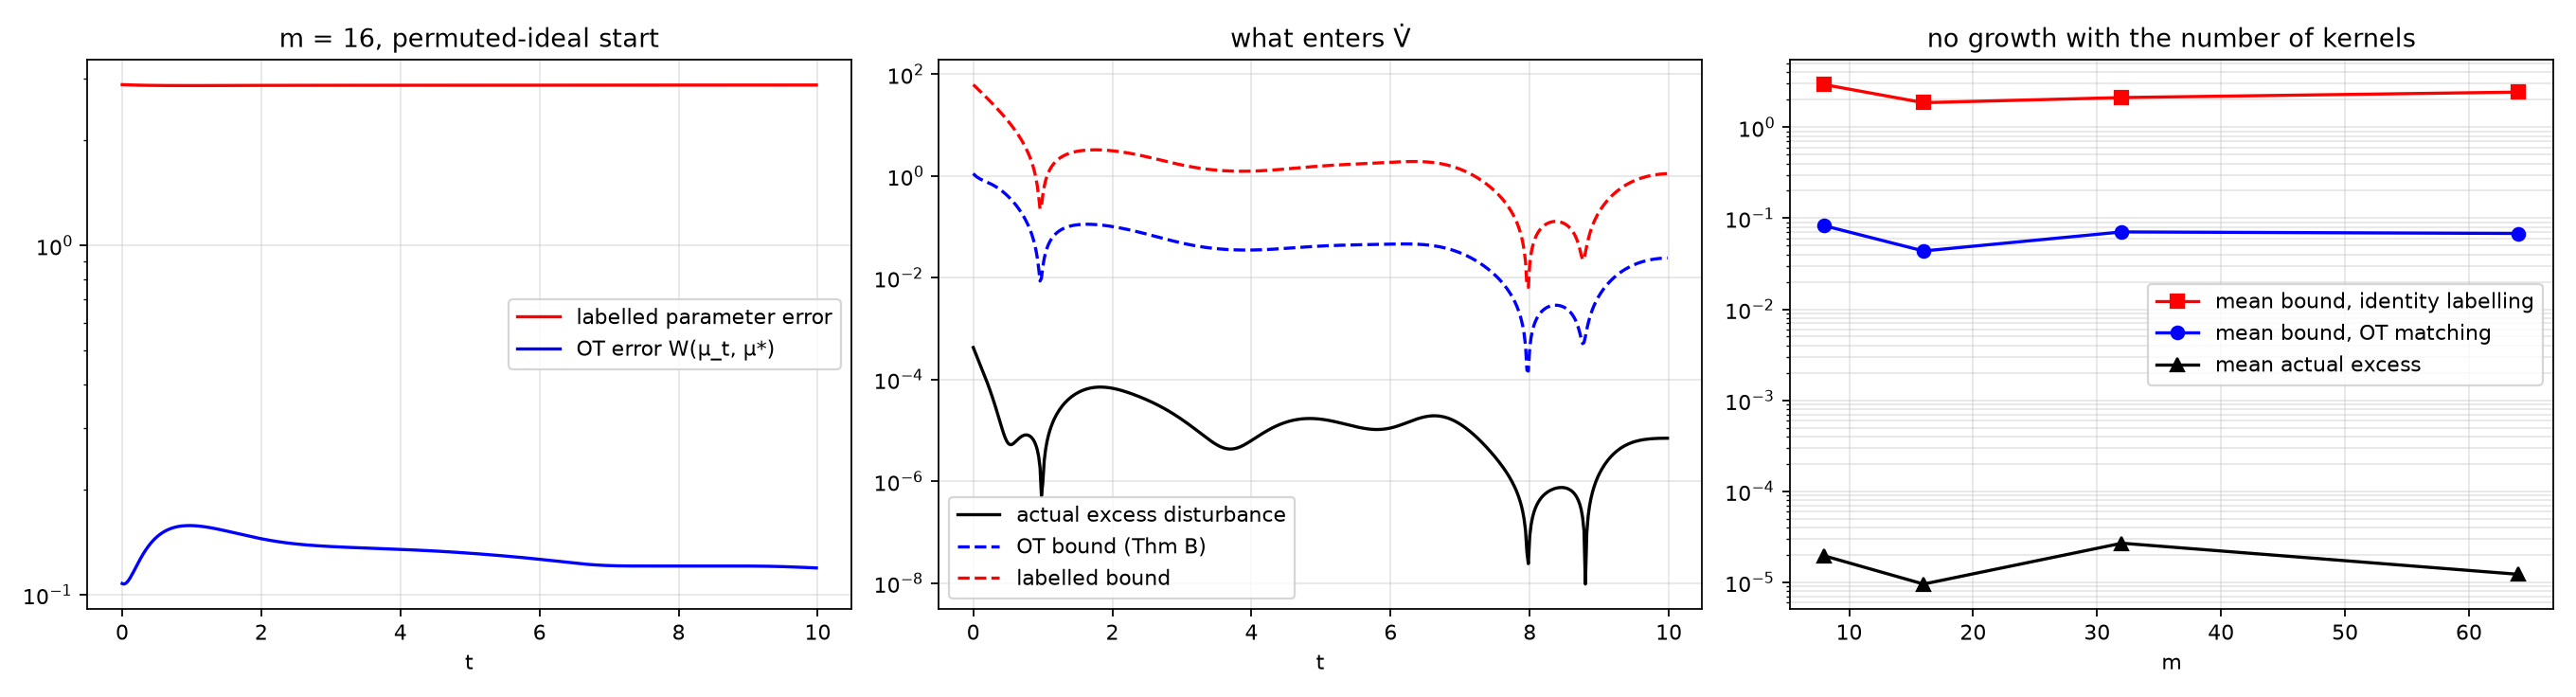
\includegraphics[width=0.95\textwidth]{transport_permutation/figure.png}
\caption{Theorem B, permuted-ideal start. Left: labelled parameter error and OT error $W(\mu_t,\mu^*)$ for $m=16$.
Centre: the actual excess disturbance that enters $\dot V$, the OT bound of Theorem B and the labelled bound, for
$m=16$. Right: the mean bound with identity labelling, the mean bound with OT matching and the mean actual excess,
against $m$.}
\label{fig:evidence:permutation}
\end{figure}

\paragraph{Corollary B.5 along \texorpdfstring{$\Lsig$}{(L-sigma)}.} This is checked by the test
\code{test_corollary_B5_fails_along_lsigma_and_its_leak_variant_holds}. The test asserts every hypothesis of C(iv) and
measures $\sup W\le\bar\eta$. There, the plain B.5 bound is exceeded by more than $3\times$, while the leak variant
with $\sigma_m b^2/4$ holds.

% ------------------------------------------------------------------------------------------------ C
\subsection{Theorem C: OT \texorpdfstring{$\sigma$}{sigma}-modification}

Scripts: \code{exp_ot_sigma_mod.py} and \code{exp_sigma_mod_transient.py} $\to$ \code{ot_sigma_mod/}.

The two starts share plant, prior, geometry and $x_0$. They differ only in particle labels
(Table~\ref{tab:evidence:sigmamod}, Figure~\ref{fig:evidence:sigmamod}). Table~\ref{tab:evidence:transient} shows
the reshuffling transient from the relabelled start (5 seeds).

\begin{table}[htbp]
\centering
\small
\caption{Theorem C: OT $\sigma$-modification against labelled $\sigma$-modification (oracle plant, $m=6$, 5 seeds,
$\sigma_m=0.3$). $\RMS\norm{e}$ is taken over $20$--$40$\,s and reported as mean $\pm$ 95\% confidence interval over seeds;
$W_{\mathrm{end}}$ is the OT error at the end.}
\label{tab:evidence:sigmamod}
\begin{tabular}{@{}llccc@{}}
\toprule
start & mechanism & $\RMS\norm{e}$ (20--40\,s) & $W_{\mathrm{end}}$ & labelled error at end\\
\midrule
aligned    & projection                 & $0.0051\pm0.0010$ & 0.2953 & 0.2953\\
aligned    & labelled $\sigma$-mod.     & $0.0091\pm0.0018$ & 0.3040 & 0.3040\\
aligned    & OT $\sigma$-mod.           & $0.0091\pm0.0018$ & 0.3040 & 0.3040\\
relabelled & projection                 & $0.0051\pm0.0010$ & 0.2953 & 0.2953\\
relabelled & labelled $\sigma$-mod.     & $0.0091\pm0.0018$ & 0.3040 & \textbf{2.0590}\\
relabelled & OT $\sigma$-mod.           & $0.0091\pm0.0018$ & 0.3040 & 0.3040\\
\bottomrule
\end{tabular}
\end{table}

\begin{table}[htbp]
\centering
\small
\caption{Reshuffling transient from the relabelled start ($m=6$, 5 seeds, $\sigma_m=0.3$): $\RMS\norm{e}$ over
time windows, and the particle path length.}
\label{tab:evidence:transient}
\begin{tabular}{@{}lccccc@{}}
\toprule
leak & $[0,5]$\,s & $[5,10]$\,s & $[10,20]$\,s & $[20,40]$\,s & particle path length\\
\midrule
labelled & 0.0771 & 0.0086 & 0.0093 & 0.0091 & 2.2585\\
OT       & 0.0743 & 0.0072 & 0.0093 & 0.0091 & 0.3917\\
\bottomrule
\end{tabular}
\end{table}

\begin{itemize}
  \item The labelled leak's longer path costs only about 4\% of early $\RMS\norm{e}$. Theorem F does not price
    leak-driven transport (Proposition C.5).
  \item The C(iv) instance in the tests satisfies every hypothesis, asserted. $\VOT$ stays below the envelope
    $e^{-\alpha t}V(0)+\beta/\alpha$ at every sample and contracts by more than $5\times$.
  \item The C(ii) test asserts $C\le b^2+4\eta R$, $\sqrt C\le b+2\eta$, and $C=b^2$ under both gap conditions, on
    300 configurations.
\end{itemize}

\begin{figure}[htbp]
\centering
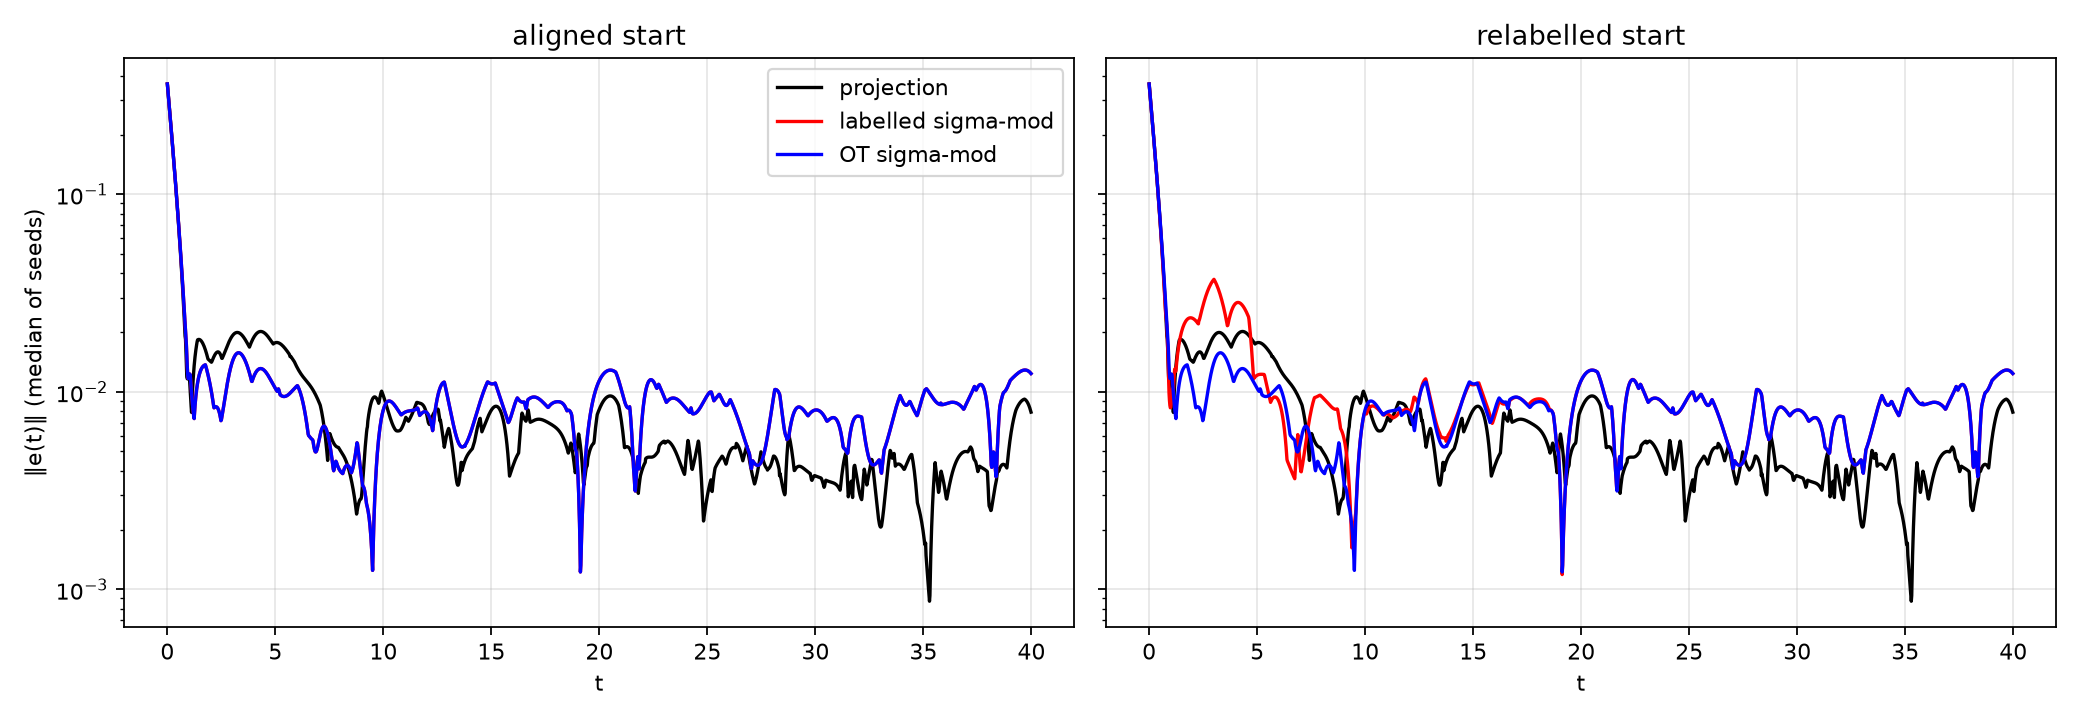
\includegraphics[width=0.9\textwidth]{ot_sigma_mod/figure.png}
\caption{Theorem C: $\norm{e(t)}$ (median of seeds) for projection, labelled $\sigma$-modification and OT
$\sigma$-modification, from the aligned start (left) and from the relabelled start (right).}
\label{fig:evidence:sigmamod}
\end{figure}

% ------------------------------------------------------------------------------------------------ D
\subsection{Theorem D: convergence in \texorpdfstring{$m$}{m}}

Script: \code{exp_mean_field_m.py} $\to$ \code{mean_field_m/}. Table~\ref{tab:evidence:meanfield} and
Figure~\ref{fig:evidence:meanfield} show the results.

\begin{table}[htbp]
\centering
\small
\caption{Theorem D: mean-field consistency in $m$ (Van der Pol plant, mean-field gains, smooth initial measure
quantised at $m$ points). The ratio is $W(\mu^m_T,\mu^{2m}_T)/W(\mu^m_0,\mu^{2m}_0)$.}
\label{tab:evidence:meanfield}
\begin{tabular}{@{}lcccc@{}}
\toprule
$m$ & $\sup_t\norm{e^m-e^{2m}}$ & $W(\mu^m_0,\mu^{2m}_0)$ & $W(\mu^m_T,\mu^{2m}_T)$ & ratio\\
\midrule
16 vs 32   & 0.0046 & 0.2179 & 0.3658 & 1.68\\
32 vs 64   & 0.0009 & 0.1091 & 0.1788 & 1.64\\
64 vs 128  & 0.0001 & 0.0545 & 0.0920 & 1.69\\
128 vs 256 & 0.0000 & 0.0273 & 0.0459 & 1.68\\
\bottomrule
\end{tabular}
\end{table}

This is a consistency check in $m$, not a check of the constant.
\begin{itemize}
  \item The guaranteed factor $e^{\Lambda T}$ is at least $e^{496}$ on this box.
  \item The Van der Pol plant fails the tube condition of Theorem D(b), so the run is covered by the localised D(d).
\end{itemize}

\begin{figure}[htbp]
\centering
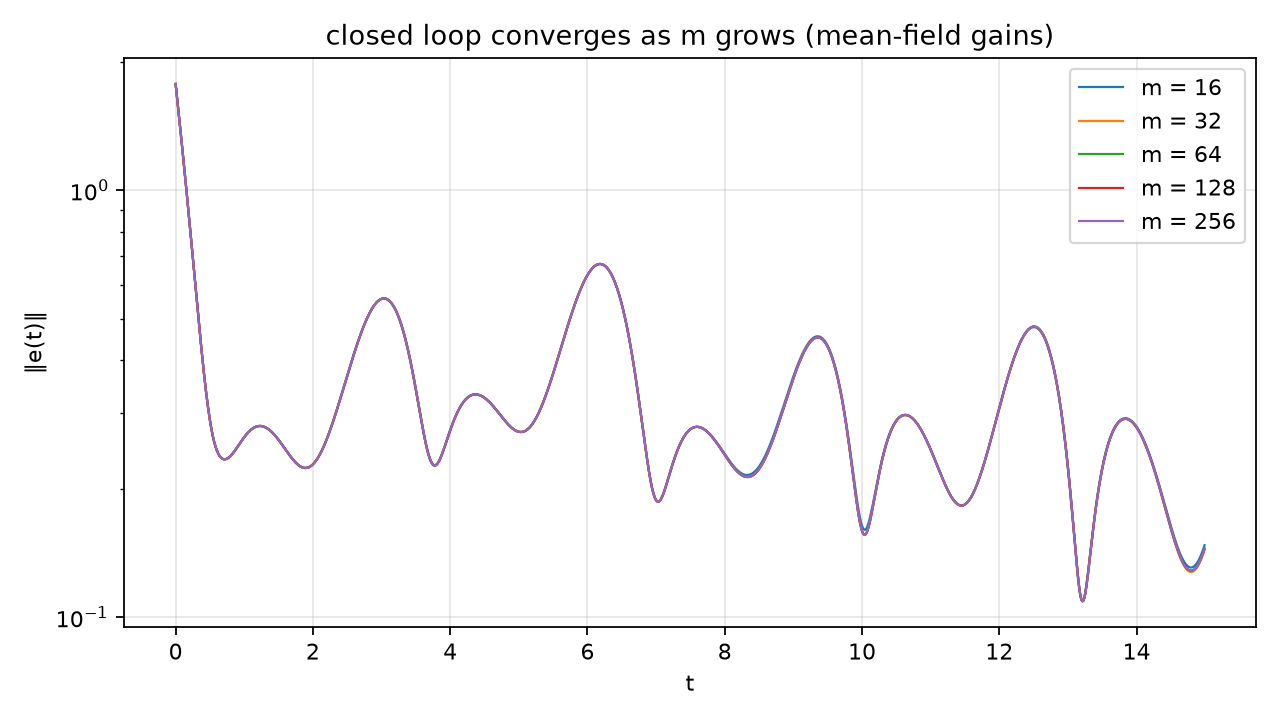
\includegraphics[width=0.8\textwidth]{mean_field_m/figure.png}
\caption{Theorem D: tracking error $\norm{e(t)}$ of the closed loop (Van der Pol plant, mean-field gains) for
$m=16$, $32$, $64$, $128$ and $256$.}
\label{fig:evidence:meanfield}
\end{figure}

% ------------------------------------------------------------------------------------------------ E
\subsection{Theorem E: label-free convergence under excitation}

Script: \code{exp_pe_convergence.py} $\to$ \code{pe_convergence/}. Table~\ref{tab:evidence:pe} and
Figure~\ref{fig:evidence:pe} show the results.

\begin{table}[htbp]
\centering
\footnotesize
\caption{Theorem E: tangential excitation and label-free parameter convergence ($m=3$, $n=2$, permuted start,
$T=200$\,s). $\lambda_{\min}$ is that of the excitation Gramian.}
\label{tab:evidence:pe}
\begin{tabularx}{\textwidth}{@{}lc*{5}{Y}@{}}
\toprule
reference & seed & $\lambda_{\min}$, first 60\,s window & min over sliding 60\,s windows & $W(T)/W(0)$
  & fitted rate of $W$, $t\ge100$\,s (1/s) & labelled$(T)$\,/ labelled$(0)$\\
\midrule
rich (6 tones) & 0 & $8.60\cdot10^{-3}$ & $4.12\cdot10^{-3}$ & 0.544 & $2.31\cdot10^{-3}$ & 0.992\\
rich (6 tones) & 1 & $5.52\cdot10^{-3}$ & $1.02\cdot10^{-3}$ & 0.409 & $2.32\cdot10^{-3}$ & 0.962\\
rich (6 tones) & 2 & $1.08\cdot10^{-3}$ & $5.91\cdot10^{-4}$ & 0.369 & $3.07\cdot10^{-3}$ & 1.007\\
single sine    & 0 & $2.54\cdot10^{-2}$ & $2.41\cdot10^{-2}$ & 0.274 & $4.05\cdot10^{-3}$ & 0.988\\
single sine    & 1 & $2.96\cdot10^{-2}$ & $2.71\cdot10^{-2}$ & 0.314 & $4.26\cdot10^{-3}$ & 0.967\\
single sine    & 2 & $6.74\cdot10^{-3}$ & $6.61\cdot10^{-3}$ & 0.226 & $2.91\cdot10^{-3}$ & 1.008\\
\bottomrule
\end{tabularx}
\end{table}

\begin{itemize}
  \item The matched error decays in all six runs. The labelled error stays within 4\% of its initial value.
  \item The rank correlation between the uniform excitation level and the fitted rate is 0.60 over the six runs. The
    PE level is a hypothesis of Theorem E, not a rate predictor (Remark E.1).
  \item The proof's linearisation is checked exactly: the Jacobian equals $A(t)$, and
    $QA+A^\T Q=\operatorname{diag}(-k_eI,0)$.
\end{itemize}

\begin{figure}[htbp]
\centering
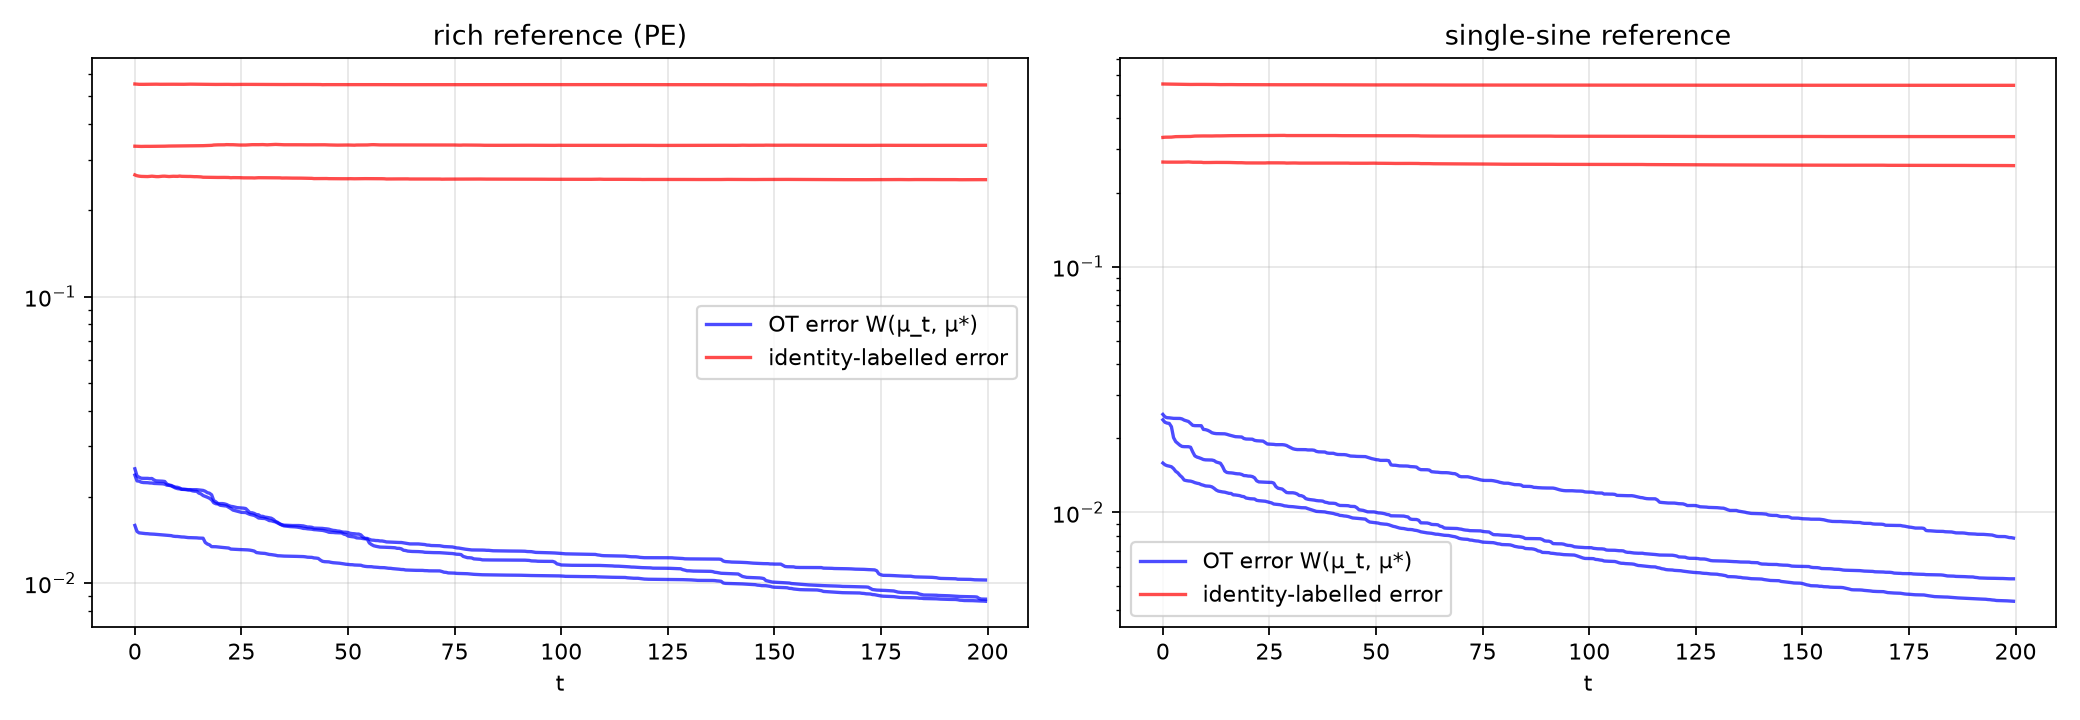
\includegraphics[width=0.9\textwidth]{pe_convergence/figure.png}
\caption{Theorem E: OT error $W(\mu_t,\mu^*)$ and identity-labelled error for the three seeds, with the rich
reference (left) and the single-sine reference (right).}
\label{fig:evidence:pe}
\end{figure}

% ------------------------------------------------------------------------------------------------ F
\subsection{Theorem F: transport cost}

Theorem F is checked by tests.
\begin{itemize}
  \item Along (L), the particle path length (which is at least the Wasserstein length) stays below
    $\lambda_G^{1/2}L_1\int\norm{e}$ at every sample.
  \item Along $\Lsig$ with the OT leak, $W(\mu_{t_1},\mu_{t_0})\le\int(\lambda_G^{1/2}L_1\norm{e}+\sigma_mW(\mu_r,\mu^0))$
    on a grid of pairs.
  \item Lemma P.1 holds on 2000 adversarial states, and a tight instance of F(i) reaches ratio $\ge0.99$.
\end{itemize}

% ------------------------------------------------------------------------------------------------ G
\subsection{Proposition G: slow geometry}

Scripts: \code{exp_variable_projection.py} and \code{exp_slow_manifold_slope.py}, both $\to$
\code{variable_projection/}.

In Table~\ref{tab:evidence:varpro}, ranges are along the run (5 samples), and ``$a$\,/\,$b$'' means
first-quarter\,/\,last-quarter medians. Velocities are centred differences of period means.

\begin{table}[htbp]
\centering
\small
\caption{Proposition G: the two configurations, \texttt{violating} ($m=4$, $k_e=20$, $g_a=2$, $\delta=0.1$,
$T=800$\,s) and \texttt{satisfying} ($m=2$, $k_e=20$, $g_a=13$, $\delta=0.004$, $T=3000$\,s). In the rows for $L^*$
and $\bar L$, ``$x\to y$'' is first sample $\to$ last sample.}
\label{tab:evidence:varpro}
\begin{tabularx}{\textwidth}{@{}>{\raggedright\arraybackslash}p{0.3\textwidth}YY@{}}
\toprule
quantity & violating ($m=4$) & satisfying ($m=2$)\\
\midrule
(H2a) $\omega_{\mathrm{ref}}$\,/\,joint fastest & 15.3--25.6 & 6.53--7.27\\
(H2b) slowest weight\,/\,geometry & 0.0993--0.231 & 78.8--87.2\\
(H2c) $S$ & 5.44--25 & 0.00601--0.00602\\
G(a) direct check (cosine, $\Ginv$ metric) & 0.9994\,/\,0.9985 & 0.9848\,/\,0.9624 (geometry block
  0.9992\,/\,0.9982)\\
G(b) cosine & $-0.118$\,/\,0.385 & 0.999\,/\,0.999\\
G(b) size ratio & 4.207\,/\,0.472 & 0.969\,/\,0.970\\
$L^*$ & \textbf{increases} ($3.8136\cdot10^{-3}\to5.8866\cdot10^{-3}$) & decreases
  ($1.1987\cdot10^{-2}\to4.1073\cdot10^{-3}$)\\
$\bar L$ at period-mean weights & non-increasing ($0.21892\to0.0080127$) & non-increasing\\
\bottomrule
\end{tabularx}
\end{table}

\paragraph{Slope counterexample.} Table~\ref{tab:evidence:slope} (\code{table_slope.md}). Here $m=1$, $k_e=20$,
gains $(g_a,\delta,\delta)$, and (H2b) holds in every row. The closed loop and the joint flow start on the slow
manifold of (b$'$).

\begin{table}[htbp]
\centering
\footnotesize
\caption{Proposition G(b): closed loop against the averaged predictions. ``closed\,/\,(b)'' compares the closed loop
with plain variable projection (VarPro) G(b), and ``closed\,/\,(b$'$)'' with the induced-metric flow G(b$'$); size
is the ratio of displacement norms.}
\label{tab:evidence:slope}
\setlength{\tabcolsep}{4pt}
\begin{tabularx}{\textwidth}{@{}>{\raggedright\arraybackslash}X*{8}{c}@{}}
\toprule
case & (H2b) & $S$ & \multicolumn{2}{c}{closed\,/\,(b)} & \multicolumn{2}{c}{closed\,/\,(b$'$)}
  & (a)\,/ & closed\,/\\
\cmidrule(lr){4-5}\cmidrule(lr){6-7}
 & ratio & & size & cosine & size & cosine & (b$'$) & (a)\\
\midrule
$\delta=0.47$, $g_a=20$ & 81--178 & 2--2.81 & 0.422 & $0.9303^{\dagger}$ & 1.121 & 0.9986 & 1.015 & 1.104\\
$\delta=0.47/4$, $g_a=5$ (all gains $\div4$) & 81--178 & 2--2.81 & 0.401 & 0.9156 & 1.065 & 0.9999 & 1.015 & 1.049\\
$\delta=0.047$, $g_a=20$ & 654--1779 & 0.2--0.319 & 0.850 & 0.9986 & 1.047 & 1.0000 & 1.003 & 1.044\\
$\delta=0.0047$, $g_a=20$ & 13162--17790 & 0.02--0.0229 & 1.023 & 1.0000 & 1.044 & 1.0000 & 1.000 & 1.044\\
\bottomrule
\multicolumn{9}{@{}l}{$^{\dagger}$The centre moves the opposite way.}
\end{tabularx}
\end{table}

\begin{itemize}
  \item (a)\,/\,(b$'$) isolates the $O(1/R)$ error of the induced-metric flow.
  \item closed\,/\,(a) isolates the averaging error, which shrinks with the gains, plus a 4.4\% $O(1/k_e)$
    error-channel factor.
\end{itemize}

What the tables show:
\begin{itemize}
  \item G(b) holds in the satisfying configuration, where (H2b) and $S\ll1$ both hold. The violating configuration
    fails both.
  \item The slope rows show that (H2b) alone is not sufficient.
  \item The induced-metric flow G(b$'$) tracks the closed loop at every $S$.
  \item In the satisfying configuration, the G(a) weight block is dominated by the $O(1/k_e)$ shift of the weight
    equilibrium: cosine $-0.21$\,/\,$0.50$, carrying 92--95\% of the residual. The geometry block matches.
\end{itemize}

\begin{figure}[htbp]
\centering
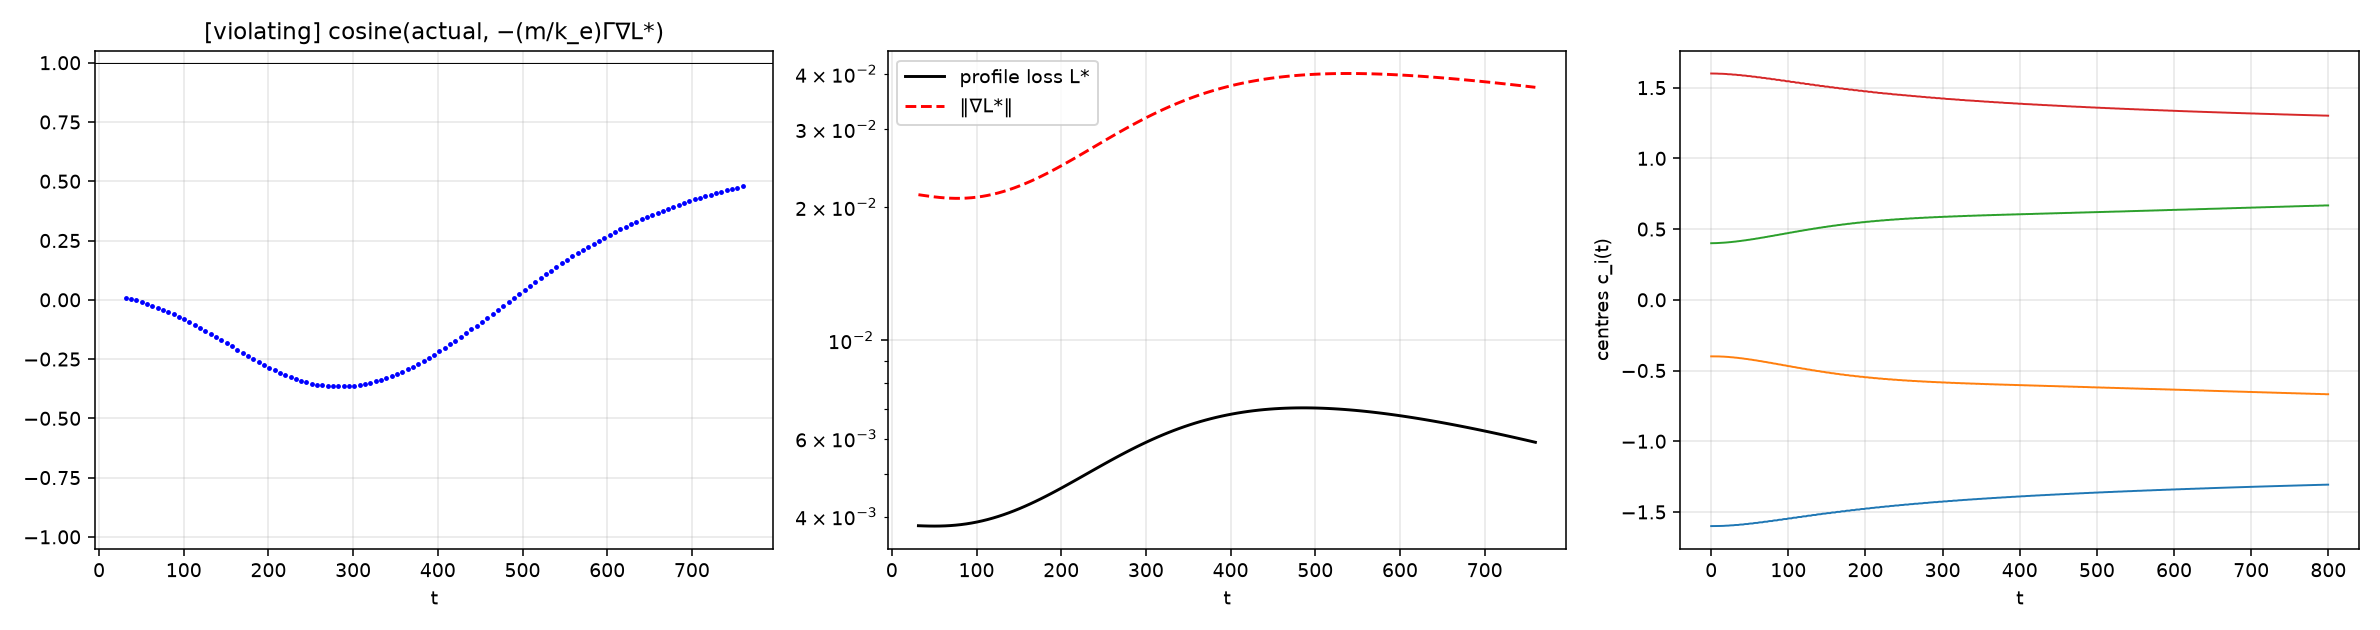
\includegraphics[width=0.95\textwidth]{variable_projection/figure_violating.png}
\caption{Proposition G, \texttt{violating} configuration. Left: the G(b) cosine between the actual geometry velocity
and the VarPro direction $-(m\delta/k_e)\Gamma\nabla L^*$, along the run. Centre: the profile loss $L^*$ and
$\norm{\nabla L^*}$. Right: the centres $c_i(t)$.}
\label{fig:evidence:violating}
\end{figure}

\begin{figure}[htbp]
\centering
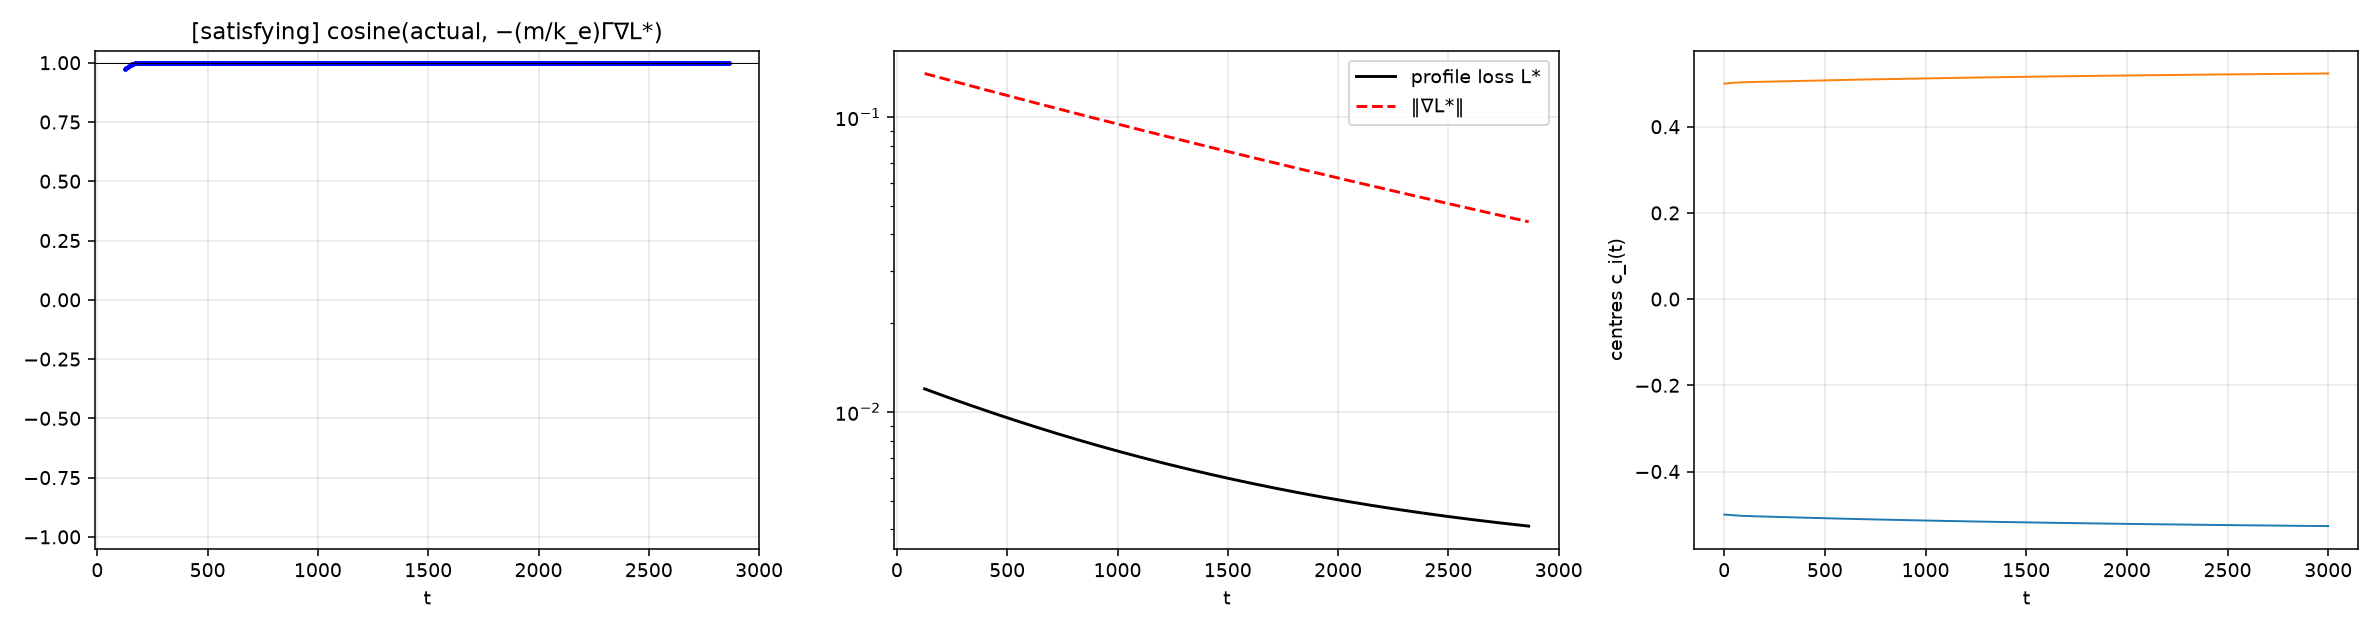
\includegraphics[width=0.95\textwidth]{variable_projection/figure_satisfying.png}
\caption{Proposition G, \texttt{satisfying} configuration; panels as in
Figure~\ref{fig:evidence:violating}.}
\label{fig:evidence:satisfying}
\end{figure}

% ------------------------------------------------------------------------------------------------ H
\subsection{Theorem H: Langevin adaptive control}

\begin{sloppypar}
\noindent Scripts: \code{exp_langevin_global.py} $\to$ \code{langevin_global/}, \code{exp_langevin_tradeoff.py}
$\to$ \code{langevin_tradeoff/}, and \code{exp_gibbs_reference.py} $\to$
\code{langevin_global/gibbs_reference.md}.
\end{sloppypar}

The setting is the real closed loop with $m=32$, a scalar plant and a periodic reference.
\begin{itemize}
  \item The unregularised offline optimum of the occupation loss is about $7.6\cdot10^{-6}$ (best of 5 L-BFGS
    restarts, an upper bound). One run gave $7.0\cdot10^{-6}$, because of floating-point summation order.
  \item \begin{sloppypar}The regularised optimum $\bar L(\mu^*_\tau)$ is $0.11118$ at $(\sigma,\tau)=(0.02,0.004)$
    and $0.00850$ at $(0.002,5\cdot10^{-4})$, grid-converged (\code{exp_gibbs_reference.py} $\to$
    \code{langevin_global/gibbs_reference.md}).\end{sloppypar}
  \item In the scaling $\sigma=0.2/k_e$, $\tau=0.04/k_e$ of Conjecture H.6, $\bar L(\mu^*_\tau)=0.11118$ for every
    $k_e$. The exactly averaged stationary state gives $\bar L=0.11415$, $0.11148$ and $0.11101$ at $k_e=10$, $20$
    and $40$. The $L^2(\rho)$ distance between the two learned functions is $6.81\cdot10^{-3}$,
    $1.43\cdot10^{-3}$ and $9.7\cdot10^{-4}$.
\end{itemize}

\paragraph{Speed--bias trade-off.} Table~\ref{tab:evidence:tradeoff} and Figure~\ref{fig:evidence:tradeoff}
($\sigma=0.002$, 2 seeds, \code{langevin_tradeoff/table.md}).

\begin{table}[htbp]
\centering
\small
\caption{Theorem H: speed--bias trade-off of parameter dither ($m=32$, $\sigma=0.002$, $k_e=10$, $T=1500$\,s,
2 seeds). The escape time is the first sample at which the collapsed run's loss is at most twice the spread run's
final loss (same seed); per-seed values are listed, and $\infty$ means not within the horizon. The losses are the
final values of $\bar L$.}
\label{tab:evidence:tradeoff}
\begin{tabular}{@{}lccc@{}}
\toprule
$\tau$ & escape of the collapsed start (s) & loss, collapsed & loss, spread\\
\midrule
0                    & $\infty$, $\infty$ & 0.166  & 0.00696\\
0.0005               & $\infty$, 1050     & 0.0249 & 0.0109\\
0.001                & 1480, 1005         & 0.0216 & 0.0148\\
0.002                & 1115, 800          & 0.0288 & 0.0233\\
0.004                & 970, 430           & 0.0392 & 0.0362\\
0.008                & 390, 295           & 0.0603 & 0.0653\\
annealed (hot start) & 990, 530           & 0.0317 & 0.0320\\
\bottomrule
\end{tabular}
\end{table}

\begin{itemize}
  \item \textbf{Fit.} The seed-averaged escape time fits $A+B\log(1/\tau)$ with an RMS relative residual of 0.045,
    against 0.253 for an Arrhenius fit. On the eight per-seed values both laws fit poorly (0.274 and 0.330). The
    data do not identify the escape mechanism, and the ``saddle'' reading of an earlier version of this analysis is
    withdrawn (Remark H.2).
  \item \textbf{Caveats.} The threshold grows with $\tau$, and the censored $\tau=5\cdot10^{-4}$ point is excluded
    from the fit.
  \item \textbf{Guaranteed rate.} The Holley--Stroock~\cite{hs1987} rate $2\tau\rho_\tau$ is at least
    $e^{-8401}$\,s$^{-1}$ at $(0.002,5\cdot10^{-4})$ and at least $e^{-1053}$\,s$^{-1}$ at $(0.02,0.004)$.
\end{itemize}

\begin{figure}[htbp]
\centering
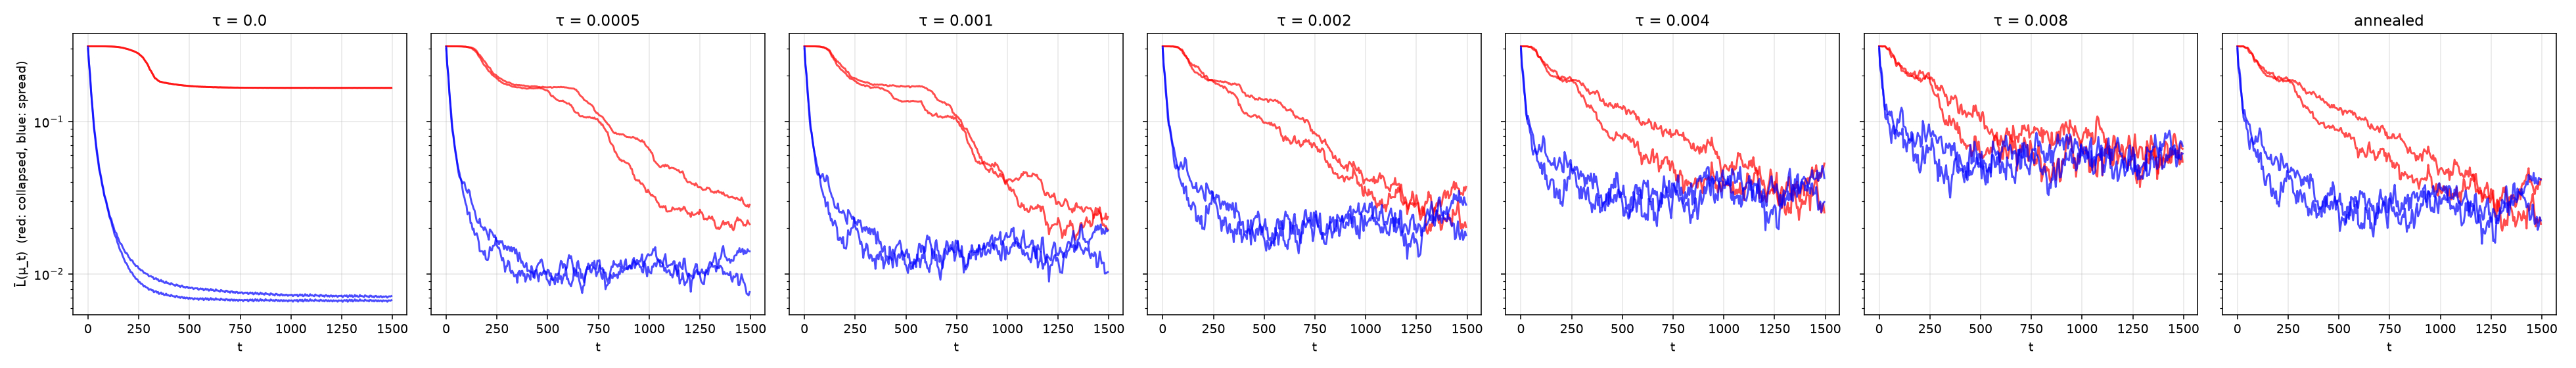
\includegraphics[width=\textwidth]{langevin_tradeoff/figure.png}
\caption{Theorem H, speed--bias trade-off: $\bar L(\mu_t)$ of the collapsed start (red) and of the spread start
(blue), 2 seeds, for $\tau=0$, $0.0005$, $0.001$, $0.002$, $0.004$, $0.008$ and the annealed (hot-start) schedule.}
\label{fig:evidence:tradeoff}
\end{figure}

\paragraph{Two fixed settings.} Three seeds (\code{langevin_global/table_*.md}; Figure~\ref{fig:evidence:global}).
\begin{itemize}
  \item \textbf{$\sigma=0.02$, $\tau=0.004$.} Both starts equalise: the loss ratio is 1.03, and the final measures
    are $4.2\times$ closer in $W$ than without dither. The common loss is about 0.11, which matches the grid value
    $\bar L(\mu^*_\tau)=0.111$. It is dominated by the regularisation bias.
  \item \textbf{$\sigma=0.002$, $\tau=5\cdot10^{-4}$.} Dither frees the collapsed start ($0.166\to0.0480$), but the
    starts do not equalise within 900\,s (loss ratio 5.23).
\end{itemize}

\begin{figure}[htbp]
\centering
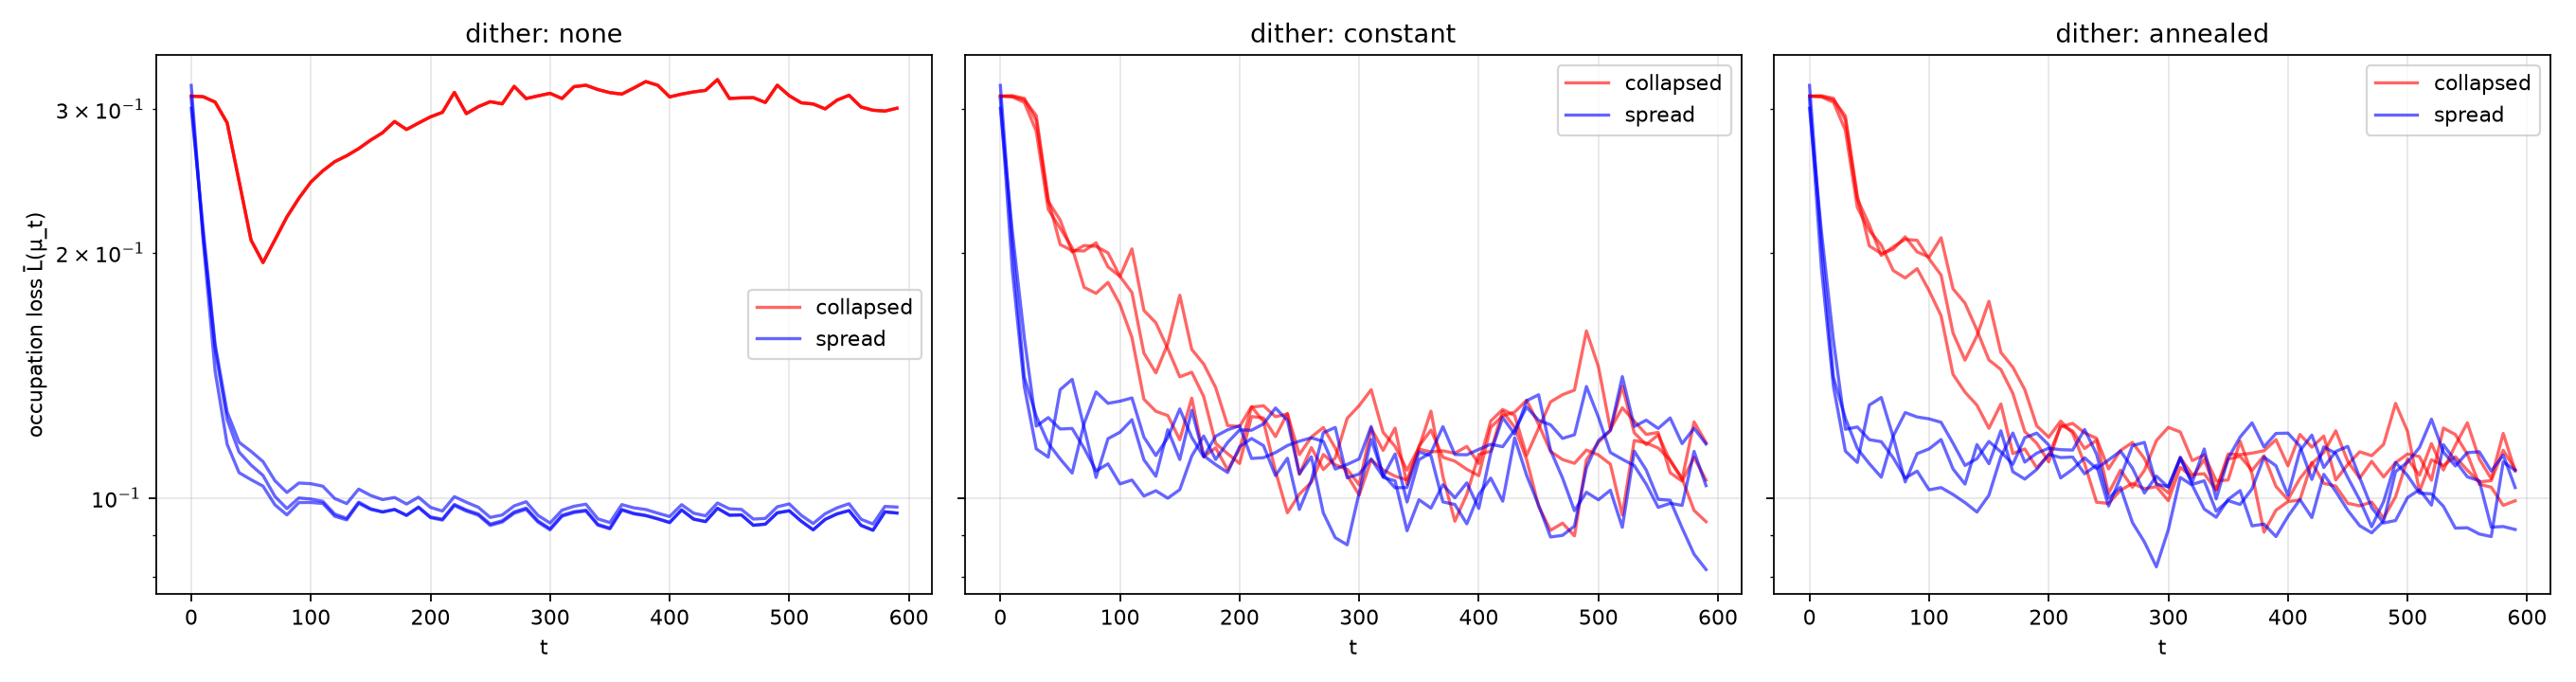
\includegraphics[width=0.95\textwidth]{langevin_global/figure_sigma0.02_tau0.004.png}\\[2pt]
{\small (a) $\sigma=0.02$, $\tau=0.004$}\\[6pt]
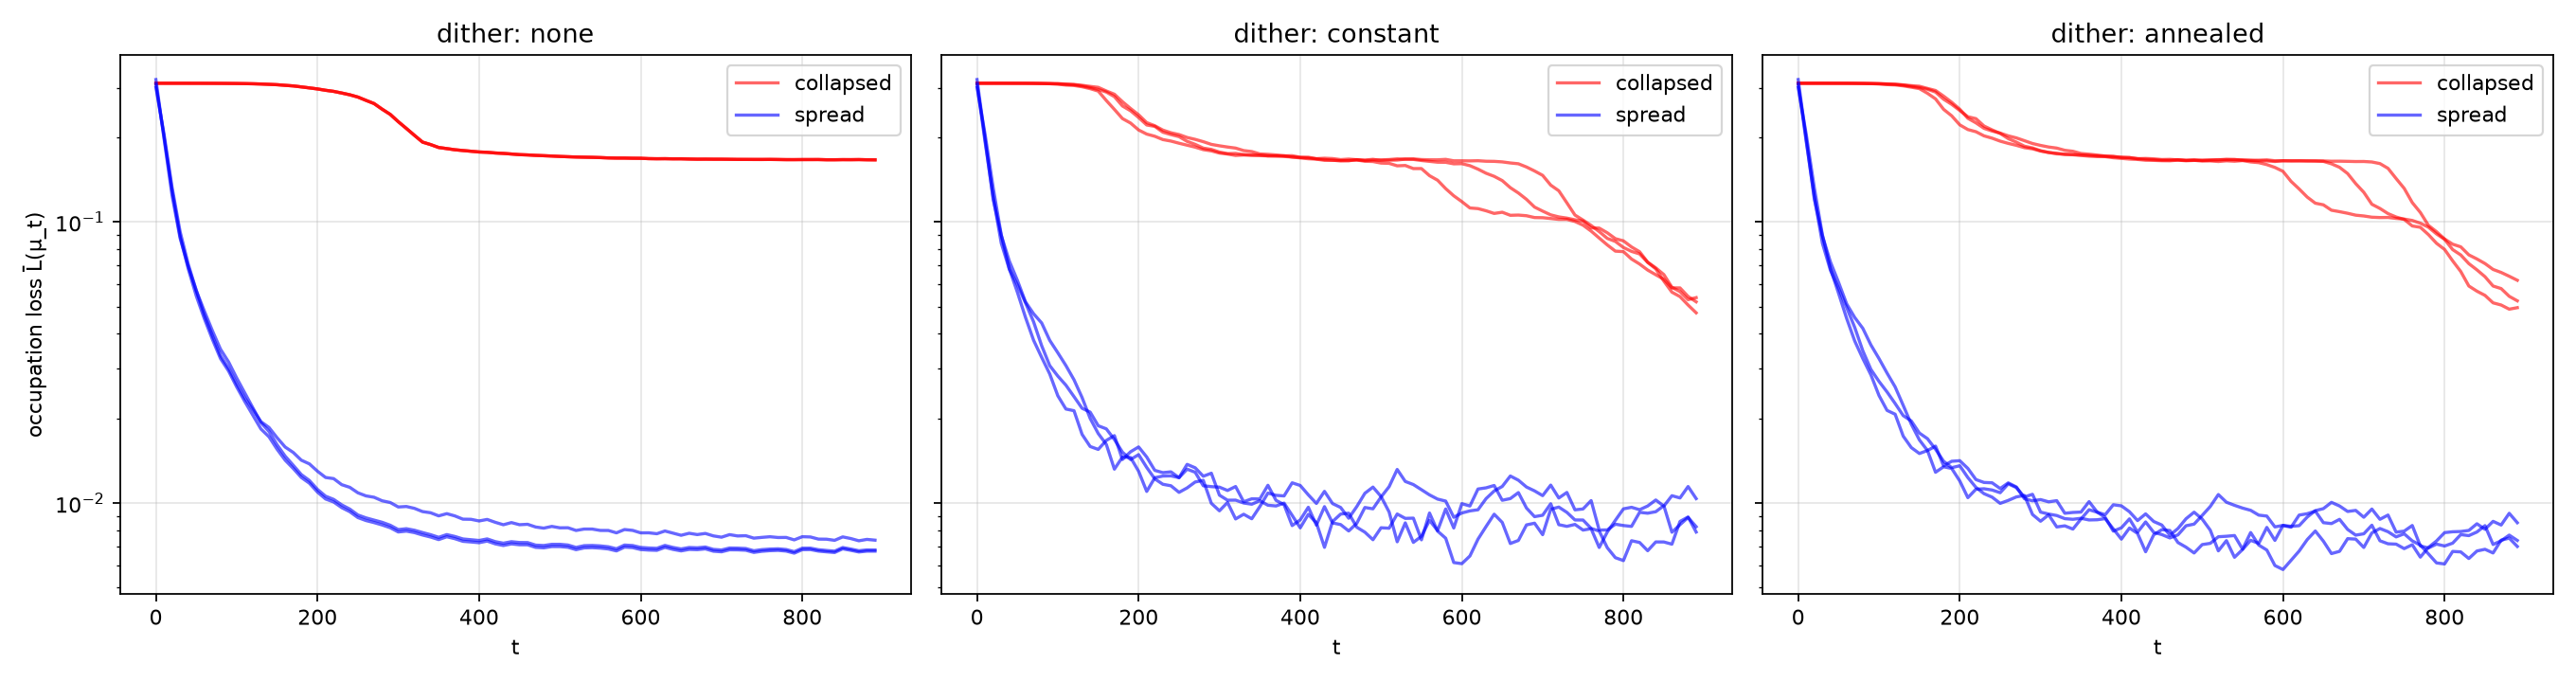
\includegraphics[width=0.95\textwidth]{langevin_global/figure_sigma0.002_tau0.0005.png}\\[2pt]
{\small (b) $\sigma=0.002$, $\tau=5\cdot10^{-4}$}
\caption{Theorem H, global kernel placement ($m=32$, scalar plant, $k_e=10$, 3 seeds): the occupation loss
$\bar L(\mu_t)$ of the collapsed and spread starts without dither, with constant dither and with annealed dither.}
\label{fig:evidence:global}
\end{figure}

% ------------------------------------------------------------------------------------------------ H.0 / H.7
\subsection{Remark H.0 and Proposition H.7: the exactly averaged closed loop}

These are checked by tests. Table~\ref{tab:evidence:averaging} gives the relative error of the frozen-$\mu$ averaged
drift against $\Aavg$, and Table~\ref{tab:evidence:structure} the structure of the first correction
(\code{test_averaging.py}).

\begin{center}
\begin{minipage}{\textwidth}
\centering
\small
\captionsetup{position=top}
\captionof{table}{Remark H.0: relative error of the frozen-$\mu$ averaged drift against $\Aavg$.}
\label{tab:evidence:averaging}
\begin{tabular}{@{}lccccc@{}}
\toprule
instance & $k_e=10$ & 20 & 40 & 80 & $k_e\times{}$error\\
\midrule
$n=1$ (\code{test_langevin.py}) & 4.2\% & 2.0\% & 0.91\% & 0.48\% & $\approx0.4$\\
$n=2$, ellipse (\code{test_averaging.py}) & 43\% & 21\% & 10\% & 5.1\% & $\approx4.2$\\
\bottomrule
\end{tabular}
\end{minipage}
\end{center}

\begin{center}
\begin{minipage}{\textwidth}
\small
\captionsetup{position=top}
\captionof{table}{Proposition H.7: structure of the first correction (\texttt{test\_averaging.py}).}
\label{tab:evidence:structure}
\begin{tabularx}{\textwidth}{@{}>{\raggedright\arraybackslash}p{0.4\textwidth}YY@{}}
\toprule
check & $n=1$ & $n=2$ (ellipse)\\
\midrule
expansion error of $k_e^2(P_\mu-P_0)$ against $U_{\mathrm{even}}+U_{\mathrm{odd}}$, $k_e=40\to80$
  & $0.54\to0.25$ & $0.038\to0.019$\\
circulation kernel $K$ & $\equiv0$ (asserted at $10^{-12}$) & antisymmetric; equals the enclosed-area integral to
  $7\cdot10^{-15}$ (asserted at $10^{-6}$)\\
orbit reversal (same $\rho$) & $U_{\mathrm{odd}}\equiv0$ & $U_{\mathrm{even}}$ unchanged, $U_{\mathrm{odd}}$
  flipped, to $2\cdot10^{-15}$ (asserted at $10^{-10}$)\\
$k_e^2\cdot{}$cyclic sum of the antisymmetric second variation, exact ($k_e=80$) against predicted (asserted at
  3\%; the full matrix at 5\%) & $-0.0711$ against $-0.0704$ & $-0.0471$ against $-0.0464$\\
\bottomrule
\end{tabularx}
\end{minipage}
\end{center}

% ------------------------------------------------------------------------------------------------ H.7a
\subsection{Remark H.7a: the orientation of the reference orbit}

Script: \code{exp_orbit_orientation.py} $\to$ \code{orbit_orientation/}.

The setup is deterministic: $n=2$, $m=6$, $G=\operatorname{diag}(4,4,1,1,1)$, $\sigma=2/k_e$, no dither. The same
elliptic reference is traversed both ways, so the occupation measure is the same, and so is the initial
configuration. The runs converged to machine precision: the residual drift over the last 10 periods is about
$10^{-16}$ (between $1.0\cdot10^{-16}$ and $5.0\cdot10^{-16}$). The six kernels converge to a common configuration
(kernel spread $1.05$ at the start, at most $5.6\cdot10^{-17}$ at the end of every run), so the learned network is
effectively a single kernel and the test probes the effect at a collapsed equilibrium. Predictions are linear responses at the $(+)$
equilibrium (Table~\ref{tab:evidence:orientation}).

\begin{table}[htbp]
\centering
\small
\caption{Remark H.7a: orientation dependence of the learned kernels in the real closed loop. Size ratios are
measured\,/\,predicted.}
\label{tab:evidence:orientation}
\begin{tabular}{@{}cccccc@{}}
\toprule
 & & \multicolumn{2}{c}{frozen-measure prediction (H.7)} & \multicolumn{2}{c@{}}{full prediction (H.7 +
  oscillation term)}\\
\cmidrule(lr){3-4}\cmidrule(l){5-6}
$k_e$ & measured $\norm{\Theta_+-\Theta_-}$ & size ratio & cosine & size ratio & cosine\\
\midrule
10 & $5.729\cdot10^{-3}$ & 2.670 & 0.7577 & 0.937 & 0.9314\\
20 & $2.843\cdot10^{-3}$ & 2.414 & 0.8302 & 0.965 & 0.9809\\
40 & $1.403\cdot10^{-3}$ & 2.294 & 0.8631 & 0.969 & 0.9944\\
\bottomrule
\end{tabular}
\end{table}

\begin{itemize}
  \item The vector error $\norm{\text{measured}-\text{predicted}}/\norm{\text{predicted}}$ of the full prediction is
    0.364, 0.195 and 0.109 at $k_e=10$, $20$ and $40$.
  \item The measured difference scales like $k_e^{-1.01}$, against a predicted $-1$.
  \item The full first-order theory accounts for it. The frozen-measure terms alone account for less than half.
  \item A first attempt with $\sigma=0.5/k_e$ and half the horizon had not converged (residual drift about a third of
    the difference). It was discarded and rerun.
\end{itemize}

% Research program (source: PARADIGM.md section 8, lines 1740-1814).
\section{Research program}\label{sec:program}

Each branch states what is proved, what is open, and the first concrete step.

\begin{enumerate}[label=\arabic*.,leftmargin=*]

\item \textbf{Infinite-horizon averaging for McKean--Vlasov closed loops (Conjecture H.6).}
  \begin{itemize}
    \item \emph{Proved:} the averaged system converges globally and exponentially (H(ii)); the exact first correction
      at frozen measure (H.7); input-to-state stability of the averaged system (H.8).
    \item \emph{Open:} a near-identity averaging transformation for the stochastic McKean--Vlasov loop that keeps the
      frozen-measure correction valid along the moving measure, uniformly in time.
    \item \emph{First step:} the deterministic case ($\tau=0$, $\sigma>0$) at fixed $m$, where the needed averaging
      theorem is classical (Sanders--Verhulst--Murdock~\cite[Ch.~5]{svm2007}, ``averaging under attraction'').
  \end{itemize}

\item \textbf{Non-reciprocal mean-field dynamics from closed-loop learning (new; Proposition H.7).}
  \begin{itemize}
    \item \emph{Proved at a frozen measure:} the averaged adaptive dynamics is a semi-gradient flow plus a lag term
      (Proposition H.7). Along the real loop a second-order averaging term is added (Remark H.7a).
    \item Its interaction has two antisymmetric parts:
      \begin{itemize}
        \item the performative defect $A_{\mathrm{even}}$ of the state shift, which is present for every $n$ and is
          the only part for $n=1$;
        \item the circulation kernel $K$, an integral over the region that the reference orbit encloses ($n\ge2$).
      \end{itemize}
    \item Non-reciprocity is checked in the instances tested, not proved in general.
    \item \emph{Open questions:}
      \begin{itemize}
        \item Are stationary states unique beyond the perturbative regime?
        \item Can circulation be \emph{designed}, choosing the orbit's orientation and area, to break symmetric traps
          or to speed escape from the collapsed configuration?
        \item Is there a Lyapunov functional other than $F_\tau$ for the non-reciprocal flow?
      \end{itemize}
    \item \emph{Context:} the closest analogues are performative prediction~\cite{S14}, semi-gradient TD
      learning~\cite{S10}, \cite{S11} and non-reciprocal phase transitions~\cite{S12}.
    \item \emph{Done (Remark H.7a):} deterministic $n=2$ closed-loop runs with the reference traversed both ways
      (same $\rho$). The full first-order theory predicts the $O(1/k_e)$ difference of the learned kernels to 3\% in
      size and 11\% as a vector.
    \item \emph{Next steps:} the same test with dither, where the stationary state is a measure; and the design of the
      orbit's orientation and area as a control input.
  \end{itemize}

\item \textbf{Uniform-in-time propagation of chaos with a plant in the loop.}
  \begin{itemize}
    \item Theorem D is finite-horizon. Uniform-in-time results exist for mean-field Langevin dynamics~\cite{S5} and
      for shallow networks~\cite{R36}.
    \item \emph{Open:} the closed loop, where the plant couples all particles through $e$, and where (by H.7) the
      averaged interaction is not reciprocal.
  \end{itemize}

\item \textbf{Geometry of two-time-scale adaptation (Proposition G(b$'$)).}
  \begin{itemize}
    \item \emph{Proved formally, and checked:} the slow geometry follows the gradient flow of the profile loss in the
      metric induced on the slow manifold, and the slope $S$ measures the departure from plain variable projection.
    \item \emph{Open:} a rigorous long-horizon statement; the $O(1/R)$ corrections, which involve $D^2a^*$ and
      $\partial_\xi M$; gain designs that shape the induced metric.
  \end{itemize}

\item \textbf{Noiseless global convergence.}
  \begin{itemize}
    \item \emph{Open:} a closed-loop separation condition under which the noiseless flow avoids spurious stationary
      points, despite the failure of the Chizat--Bach~\cite{R29} boundary conditions. Candidates are a compactified
      width coordinate and reflecting boundaries (Remark H.3).
  \end{itemize}

\item \textbf{Unbalanced transport, meaning online structure adaptation.}
  \begin{itemize}
    \item Treat the weights as masses (Hellinger--Kantorovich\,/\,Wasserstein--Fisher--Rao) to obtain birth and death
      of kernels with Lyapunov guarantees. The conic particle descent of~\cite{R49} and~\cite{R55} is the static
      analogue.
  \end{itemize}

\item \textbf{Excitation theory in measure space.}
  \begin{itemize}
    \item \emph{Open:} the continuum form of (PE); the trajectory kernel
      \[K_T(\vartheta,\vartheta')=\int\Phi(x(s);\vartheta)\Phi(x(s);\vartheta')\dd s;\]
      identifiability of measures up to symmetry; the relation to~\cite{R16}. Remark E.1 shows that the PE level alone does not predict the rate.
      A quantitative, uniform UES estimate for the skew-symmetric class is a first target.
  \end{itemize}

\item \textbf{Transport-regularised adaptive laws.}
  \begin{itemize}
    \item Wasserstein proximal (JKO) discrete-time adaptive laws.
    \item The OT leak toward priors with a different number of atoms, using optimal plans with barycentric
      projection.
    \item Transfer: transporting a learned measure to a new plant.
  \end{itemize}

\item \textbf{Quantisation and the curse of dimensionality (Corollary B.6).}
  \begin{itemize}
    \item \emph{Open:} second-order (centroid) quantisation rates for the ideal measure on the lifted space;
      approximation rates that do not go through $W$ (Maurey-type); adaptive laws that track optimal quantisers (the
      centroidal Voronoi tessellation connection~\cite{R14}).
  \end{itemize}

\item \textbf{Symmetric systems beyond kernels.} The OT quotient applies verbatim to swarms of identical agents,
  mixtures and multi-head models (\cite{R88} and~\cite{R89} are the control-side precedents).

\item \textbf{Deep approximators.} Hierarchical (multi-layer) mean-field measures, with a layer-wise OT Lyapunov
  function.

\end{enumerate}


\appendix
% Verification map (source: PARADIGM.md section 7, version 4).
\section{Verification map}\label{sec:verification}

Table~\ref{tab:verification:map} lists the tests and experiments of the accompanying repository that check each
statement; statements not checked are listed after it. Test files are abbreviated: \code{T} is
\code{tests/test_transport.py}, \code{Lg} is \code{tests/test_langevin.py}, \code{Av} is \code{tests/test_averaging.py},
\code{Ex} is \code{tests/test_excitation.py}, \code{NR} is \code{tests/test_nonreciprocity.py}, \code{Pe} is
\code{tests/test_periodic.py} and \code{Ba} is \code{tests/test_barycentric.py}.

{\footnotesize
\begin{longtable}{@{}>{\raggedright\arraybackslash}p{0.19\textwidth}>{\raggedright\arraybackslash}p{0.41\textwidth}%
>{\raggedright\arraybackslash}p{0.34\textwidth}@{}}
\caption{Verification map.}\label{tab:verification:map}\\
\toprule
statement & what is checked & where\\
\midrule
\endfirsthead
\multicolumn{3}{@{}l}{\emph{Table~\ref{tab:verification:map}, continued}}\\
\toprule
statement & what is checked & where\\
\midrule
\endhead
\midrule
\multicolumn{3}{r@{}}{\emph{continued on the next page}}\\
\endfoot
\bottomrule
\endlastfoot
constants (1) of Section~\ref{sec:setting}, closed forms & $\nabla^2_{(c,s)}\varphi\le H_\varphi$ by brute force
  & \code{T::test_gaussian_constants_are_suprema}\\
Lemma P.1 & $\norm{\Proj(\vartheta,Gy)}_{\Ginv}\le\norm{y}_G$ on 2000 adversarial states, with equality when
  inactive; a tight instance of F(i) with ratio $\ge0.99$
  & \code{T::test_lemma_P1_projection_is_nonexpansive_and_tight_velocity_bound}\\
A(i) raw rates & lifted raw rates equal classical raw rates under the gain map ($10^{-10}$)
  & \code{T::test_identification_with_classical_law}\\
A(i) projected rates, only-if & per-kernel projection with rescaled layer matches to $10^{-10}$ with active
  projections; an unrescaled layer does not; five joint balls are each distinguished (two-case construction: four
  active against an inactive per-kernel field, one inactive against an active one)
  & \code{T::test_identification_projected_rates_per_kernel}\\
B with constant ideal and $\varepsilon=0$ & the identity to floating-point precision; cross term $\le0$; remainder
  $\le$ Lemma B.2; $\dot V_\pi\le{}$(B) at every sample
  & \code{T::test_theorem_B_inequality_along_trajectories}\\
B with a moving ideal, $\varepsilon\ne0$, switches and active projection & the same plus $V_*W$; at least one
  switch; projection active at $\ge10$ samples; Dini quotient $\le{}$(B)
  & \code{T::test_theorem_B_moving_ideal_nonrepresentable_switches_and_active_projection}\\
B, Dini form & forward-difference quotient of $\VOT\le{}$(B)
  & \code{T::test_dini_derivative_of_V_OT_bounded_by_active_branch}\\
B against labelling & matched error $\ll$ labelled error; the bound is 30--45$\times$ smaller
  & \code{T::test_permuted_ideal_labelled_vs_OT}, \code{exp_transport_permutation.py}\\
B.5: failure of the plain bound along $\Lsig$; the $\Lsig$ variant holds & with every C(iv) hypothesis asserted, the
  plain bound fails by $>3\times$ and the leak variant holds
  & \code{T::test_corollary_B5_fails_along_lsigma_and_its_leak_variant_holds}\\
C(i), Lemma C.3 (unprojected pure leak) & zero switches and exact $e^{-\sigma t}$ decay (explicit Euler, pure leak)
  & \code{T::test_theorem_C_i_exact_dissipation_pure_leak}\\
C(ii) & $C\le b^2+4\eta R$; $\sqrt C\le b+2\eta$; $C=b^2$ under both gap conditions (300 configurations)
  & \code{T::test_lemma_C_ii_induced_coupling_bound}\\
C(iv) & an instance satisfying \textbf{every} hypothesis, asserted, including the gap condition
  $4\bar\eta(b+\bar\eta)<\Delta_{\mathrm{gap}}$; the envelope holds at every sample, with actual contraction
  & \code{T::test_theorem_C_iv_exponential_estimate}\\
C(v), Proposition C.5 & label invariance of the OT leak; the reshuffling transient of the labelled leak
  & \code{exp_ot_sigma_mod.py}, \code{exp_sigma_mod_transient.py}\\
C$'$(i) & the plan reduces to the assignment for $m_0=m$ ($10^{-10}$) and
  $W^2=V_{\mathrm{bar}}^2+\mathrm{Var}_\gamma$ ($10^{-10}$); along the pure leak $W^2$ is non-increasing at every
  step and $D^+Z\le-\sigma_mV_{\mathrm{bar}}^2$ holds at every state; the flow reaches $V_{\mathrm{bar}}^2<10^{-8}$
  and ends at a fixed point of the equal-mass Lloyd iteration
  & \code{Ba::test_plan_reduces_to_assignment_and_pythagorean_split},
    \code{Ba::test_pure_barycentric_leak_dissipates_to_a_centroidal_configuration},
    \code{exp_barycentric_leak.py} $\to$ \code{results/barycentric_leak/table.md}\\
C$'$(ii) & $\sqrt{C_{\mathrm{bar}}}\le b+2\eta$ on 90 random configurations; $C_{\mathrm{bar}}=b_{\mathrm{bar}}^2$
  at small $\eta$ (plan stability)
  & \code{Ba::test_induced_coupling_bound_and_plan_stability}\\
C$'$(iii) & the Lyapunov inequality at every recorded state of a closed loop with the barycentric leak toward a
  24-atom prior
  & \code{Ba::test_lyapunov_inequality_along_the_barycentric_leak_closed_loop}\\
D & consistency in $m$ (nearly constant amplification 1.64--1.69; not the constant $e^{\Lambda T}$)
  & \code{exp_mean_field_m.py}\\
D$'$(b), (d) & the $m^{-1/2}$ rate of the synchronous coupling to a 4096-particle reference: slopes $-0.47\pm0.06$
  ($\tau=0$) and $-0.46\pm0.05$ ($\tau=2\cdot10^{-3}$) over 24 seeds, $0.94\pm0.08$ and $0.92\pm0.08$ against
  $(1/m-1/M)^{1/2}$; not the constant
  & \code{exp_chaos.py} $\to$ \code{results/chaos/table.md}\\
D$''$ & with exact Lipschitz constants and the a-priori tube, $\sigma_{\mathrm{cert}}=4.04$ against Proposition K's
  $\sigma_K=0.00144$; at $1.2\sigma_{\mathrm{cert}}$ with dither the coupled distance is of order $m^{-1/2}$ (slope
  $-0.51\pm0.02$), bounded in time and $700\times$ below the bound, with the network at its prior (fit error $1.000$);
  without dither the reference collapses (spread $10^{-14}$) and the distance is zero; at $\sigma_{\mathrm{cert}}/8$
  it decays to $10^{-11}$; in the learning regime ($\sigma_K/3$, 1000\,s) the network stays spread and fits the plant
  (fit error $0.63$) and the distance follows $m^{-1/2}$ ($-0.62\pm0.16$) but grows threefold between the windows
  $(100,200]$ and $(500,1000]$
  & \code{exp_chaos_uniform.py} $\to$ \code{results/chaos/uniform_table.md}\\
F(ii) along (L) & particle path length ($\ge$ Wasserstein length) $\le\lambda_G^{1/2}L_1\int\norm{e}$ at every sample
  & \code{T::test_theorem_F_wasserstein_length_bounded_by_integrated_error}\\
F(ii$'$) along $\Lsig$ & $W(\mu_{t_1},\mu_{t_0})\le\int(\lambda_G^{1/2}L_1\norm{e}+\sigma_mW(\mu_r,\mu^0))$ on a grid
  of pairs; a tight instance with $e\equiv0$ (ratio $\ge0.99$), where the motion is $W\approx1.05$
  & \code{T::test_theorem_F_leak_clause_along_ot_sigma_mod},
    \code{T::test_theorem_F_leak_clause_is_tight_when_the_leak_pays_for_all_motion}\\
E linearisation & Jacobian of the implemented loop equals $A(t)$; $QA+A^\T Q=\operatorname{diag}(-k_eI,0)$
  & \code{T::test_theorem_E_linearisation_and_lyapunov_identity}\\
E convergence & the matched error decays and the labelled error does not (qualitative); sliding-window excitation and
  fitted rates
  & \code{T::test_theorem_E_matched_error_converges_labelled_does_not}, \code{exp_pe_convergence.py}\\
Lemma E.0 & $p_{\mathrm{lo}}\norm{w}^2\le V\le p_{\mathrm{hi}}\norm{w}^2$ and $\dot V\le-\gamma\norm{w}^2$ at random
  $(t,w)$ for four regressors, closed-form and optimised $\varepsilon$; the envelope along trajectories; explicit
  rate $\le$ exact Floquet rate
  & \code{Ex::test_lemma_E0_pointwise_inequalities_hold_on_random_states},
    \code{Ex::test_lemma_E0_envelope_and_floquet_ordering}\\
Lemma E.0(iii), Remark E.0a & the $\omega^{-2}$ law of the explicit rate and of the exact rate; the saturation of
  exact/explicit in the slow-adaptation limit; the tables
  & \code{Ex::test_remark_E1_omega_scaling_of_the_explicit_rate},
    \code{Ex::test_slow_adaptation_limit_ratio_is_bounded}, \code{exp_explicit_rate.py} $\to$
    \code{results/explicit_rate/table.md}\\
E, explicit constants & on the implemented loop, from a start inside the explicit ball,
  $\norm{w(t)}\le(p_{\mathrm{hi}}/p_{\mathrm{lo}})^{1/2}e^{-\lambda t}\norm{w(0)}$ at every sample ($L_J$ estimated
  from samples)
  & \code{Ex::test_theorem_E_explicit_nonlinear_envelope_on_the_implemented_loop}\\
G(a), two scales & direct check (cosine $\ge0.998$ in the $\Ginv$ metric, \code{violating}; the weight block fails
  in \code{satisfying}, as explained in Section~\ref{sec:propG}); $\bar L$ at period-mean parameters
  non-increasing
  & \code{exp_variable_projection.py} $\to$ \code{table_violating.md}, \code{table_satisfying.md}\\
G(b), (b$'$), (H2c) & VarPro holds when (H2b) and $S\ll1$ hold; it fails when $S=O(1)$ although (H2b) holds; the
  induced-metric flow tracks the closed loop at every $S$ (started on the slow manifold; gains $\div4$ isolates the
  averaging error)
  & \code{exp_variable_projection.py} $\to$ \code{table_satisfying.md}; \code{exp_slow_manifold_slope.py} $\to$
    \code{table_slope.md}\\
H(i), algebraic identity & with $e:=r/k_e$ and $x:=x_m$, the averaged drift equals $-G\nabla V$ (code gradients
  against finite differences, $10^{-7}$); does not test averaging
  & \code{Lg::test_averaged_drift_is_the_mean_field_langevin_drift}\\
Remark H.0 & the frozen-$\mu$ averaging error decays like $1/k_e$, $n=1$ and $n=2$
  & \code{Lg::test_averaging_error_of_the_formal_reduction_decreases_like_one_over_ke},
    \code{Av::test_averaged_drift_error_decays_like_one_over_ke_for_an_orbit_enclosing_area}\\
H, need for entropy & finite-$m$ real loop: a noiseless symmetric start stays bit-identical (and moves); dither
  separates it
  & \code{Lg::test_noiseless_symmetric_initialisation_never_separates_but_dither_does}\\
H(ii), oscillation bound & $\abs{V_L[\mu](\vartheta)}\le K_\Phi(F_\rho+K_\Phi)$ for random and adversarial $\mu$,
  $\vartheta$
  & \code{Lg::test_first_variation_bound_used_in_holley_stroock}\\
H(ii) constant & formula transcription only & \code{Lg::test_lsi_lower_bound_formula}\\
H, global behaviour & collapsed against spread starts, with and without dither, two $(\sigma,\tau)$ settings
  & \code{exp_langevin_global.py}\\
H, speed--bias trade-off & escape time and loss floor against $\tau$; $\log(1/\tau)$ and Arrhenius fits,
  seed-averaged and per seed (neither identifies the mechanism)
  & \code{exp_langevin_tradeoff.py}\\
H, reference values & $\bar L(\mu^*_\tau)$ by a concave dual on a grid; the stationary state of the exactly averaged
  loop; their offset in the scaling of H.6
  & \code{exp_gibbs_reference.py} $\to$ \code{results/langevin_global/gibbs_reference.md}\\
H.7 & expansion, Stokes area identity, parity under reversal, non-reciprocity of the exact second variation
  & \code{Av::test_frozen_measure_expansion_converges_at_rate_one_over_ke},
    \code{Av::test_circulation_kernel_antisymmetric_vanishes_in_1d_and_equals_the_enclosed_area_integral},
    \code{Av::test_shift_correction_is_even_and_lag_correction_is_odd_under_orbit_reversal},
    \code{Av::test_exactly_averaged_dynamics_is_non_reciprocal_for_n1_and_n2}\\
H.7a, oscillation term & value against an independent one-period near-identity flow (within 3\% at $k_e=80$); odd
  under orbit reversal ($10^{-6}$)
  & \code{Av::test_oscillation_correction_matches_a_one_period_flow},
    \code{Av::test_oscillation_correction_is_odd_under_orbit_reversal}\\
I(i), (ii) & $a^\T B(\xi,\xi')a'$ equals the antisymmetric part of $S_{\mathrm{even}}+K$ ($10^{-10}$);
  $A(\vartheta,\vartheta_z)=0$ and the cyclic sum over $(\vartheta_0,\vartheta_1,\vartheta_z)$ equals
  $A(\vartheta_0,\vartheta_1)$ ($10^{-14}$)
  & \code{NR::test_bilinear_form_B_reproduces_the_antisymmetric_second_variation},
    \code{NR::test_zero_feature_collapses_the_cyclic_criterion_to_a_pairwise_one}\\
I(iii) & $n=1$: $A\equiv0$ at perfect fit ($<10^{-13}$); $A\ne0$ with a residual, equal to the closed form; the
  positivity witness
  & \code{NR::test_n1_reciprocal_iff_residual_vanishes_on_the_orbit}, \code{NR::test_positivity_witness_n1}\\
I(iv) & the closed form of $\kappa$ ($10^{-10}$); the second component of $F_s((0.5,0))$ is positive on the
  ellipse; $\kappa\equiv0$ on a zero-current orbit; with $f\equiv\fhat_\mu$ on $\R^2$ ($Dr_\mu\equiv0$)
  $B=2\kappa I$, $A\ne0$ on the ellipse and $A\equiv0$ on the segment; with $f=\fhat_\mu+he_1$, $h$ zero on the
  ellipse, the curl term survives and equals $-\int\varphi\varphi'\partial_2h\dd\rho\cdot(e_1e_2^\T-e_2e_1^\T)$
  & \code{NR::test_circulation_kernel_closed_form_and_vanishing_for_a_zero_current_orbit},
    \code{NR::test_perfect_fit_n2_leaves_only_the_circulation_kernel},
    \code{NR::test_perfect_fit_on_the_orbit_alone_keeps_the_curl_term}\\
J, averaged objective & $\nabla J_m$ against finite differences ($10^{-7}$); the critical point is a non-degenerate
  minimum with two distinct kernels
  & \code{Pe::test_gradient_of_J_m_matches_finite_differences_and_critical_point_is_nondegenerate}\\
J(a), (b), (d) & Newton shooting finds the periodic orbit (residual $<10^{-10}$); $\norm{\bar\Theta_p-\Theta^*}$
  and $\max\norm{e}$ halve from $k_e=20$ to $40$; the vector error of the first-order prediction of the offset
  halves as well (it is 0.55 at $k_e=40$ in the fast-sweep test instance, and 0.041 at $k_e=40$ in instance A of
  the experiment); the parameter Floquet exponents match $\frac1{k_e}\lambda(G_m^{1/2}\nabla^2J_mG_m^{1/2})$ with a
  maximal relative error below 2\% at $k_e=40$ that halves with $k_e$; both instances at $k_e=10$--$160$ in the
  experiment; the error-channel exponent recovered from Liouville's trace identity is $k_e-L$ with $\abs{L}<0.2$
  & \code{Pe::test_theorem_J_periodic_orbit_offset_and_floquet_exponents}, \code{exp_periodic_orbit.py} $\to$
    \code{results/periodic_orbit/table.md}\\
K(i), (ii) & the Hessian of $J_m$ at a collapsed configuration equals
  $I_m\otimes(\sigma_0\Ginv-R_2)+\frac1m(\mathbf{1}\mathbf{1}^\T)\otimes M_2$ (finite differences, $10^{-5}$ relative);
  $\sigma_{\mathrm{crit}}$ solves $\sigma=\lambda_{\max}(G^{1/2}R_2(\bar\vartheta(\sigma))G^{1/2})$ ($10^{-8}$) and
  the separation block is singular there; the separation Floquet exponents of the collapsed orbit come in
  $(m-1)$-fold multiplets
  & \code{Pe::test_proposition_K_hessian_splitting_and_critical_leak}, \code{exp_orientation_stability.py}\\
K(iii), (iv) & the orientation difference of the softest separation exponent at $\sigma_0=0.5$: slope $-2.18$
  against $k_e$, within 14\% $\to$ 3\% of the prediction at $\bar\Theta_2$ for $k_e=10\to80$, while the prediction
  at $\Theta^*$ converges to a value 30\% off; at $\sigma_{\mathrm{crit}}$ both orientations are unstable,
  predictions within 14\% at $k_e=40$; at the designed $\sigma_0$ the signs differ for $k_e=10$ and $20$
  & \code{exp_orientation_stability.py} $\to$ \code{results/orientation_stability/table.md}\\
H.7 + H.7a in the real closed loop & the orientation dependence of the learned kernels (same $\rho$) is predicted to
  within 3\% in size and 11\% as a vector, cosine 0.994 at $k_e=40$; the measured difference scales like
  $k_e^{-1.01}$
  & \code{exp_orbit_orientation.py} $\to$ \code{results/orbit_orientation/table_sigma2_slow16.md}\\
\end{longtable}
}

\noindent Not checked in the repository:
\begin{itemize}
  \item B.5 along (L), and B.6 and B.7;
  \item the Filippov form of C(i), the inequality of C(v), and Proposition C.5's $D^+\VOT=\sigma_m(\delta-\delta^2)$;
  \item D(b), D's constant, and the one-sided constant of Remark D.1;
  \item the sharpness of the explicit rate of E beyond the tables of Remark E.0a; Corollary E.2 and Remark E.3;
  \item Theorem I(v) beyond the two instances (the analytic dichotomy is a proof only);
  \item Theorem J(c) (the basin; a single basin run is reported in \code{review/REVIEW_round5_J.md});
  \item Proposition K(iii)--(iv) beyond the instance of \code{exp_orientation_stability.py}, and the second-order
    normal form it rests on;
  \item Theorem C$'$(iv) (its hypotheses are not met on any tested instance) and the convergence of the pure leak to
    a critical point beyond the tested instances; Theorem D$'$'s constant, its per-particle bound and its
    $k$-particle convergence (only the rate of (b) is checked);
  \item H.8, which is a proof only;
  \item Conjecture H.6.
\end{itemize}


\begin{thebibliography}{99}

\bibitem{R64}
S. K. Ainsworth, J. Hayase, S. Srinivasa.
\emph{Git Re-Basin: merging models modulo permutation symmetries}.
International Conference on Learning Representations (ICLR), 2023.
arXiv:2209.04836.

\bibitem{ags2008}
L. Ambrosio, N. Gigli, G. Savar\'e.
\emph{Gradient Flows in Metric Spaces and in the Space of Probability Measures}.
2nd edition, Lectures in Mathematics ETH Z\"urich. Birkh\"auser, Basel, 2008.
\url{https://doi.org/10.1007/978-3-7643-8722-8}.

\bibitem{S42}
F. Aurenhammer, F. Hoffmann, B. Aronov.
\emph{Minkowski-type theorems and least-squares clustering}.
Algorithmica, 20:61--76, 1998;
J. Kitagawa, Q. M\'erigot, B. Thibert, \emph{Convergence of a Newton algorithm for semi-discrete optimal
transport}, Journal of the European Mathematical Society, 21(9):2603--2651, 2019.

\bibitem{be1985}
D. Bakry, M. \'Emery.
\emph{Diffusions hypercontractives}.
In J. Az\'ema, M. Yor (eds.), S\'eminaire de Probabilit\'es XIX, 1983/84, Lecture Notes in Mathematics 1123,
pp.~177--206. Springer, Berlin, 1985.
\url{https://doi.org/10.1007/BFb0075847}.

\bibitem{S19}
M. Balzer, T. Schl\"omer, O. Deussen.
\emph{Capacity-constrained point distributions}.
ACM SIGGRAPH 2009;
Q. M\'erigot, \emph{A multiscale approach to optimal transport}, Computer Graphics Forum, 30(5), 2011;
F. de Goes, K. Breeden, V. Ostromoukhov, M. Desbrun, \emph{Blue noise through optimal transport},
ACM Transactions on Graphics, 31(6), 2012.

\bibitem{S2}
R. Barboni, G. Peyr\'e, F.-X. Vialard.
\emph{Ultra-fast feature learning for the training of two-layer neural networks in the two-timescale regime}.
arXiv:2504.18208, 2025.

\bibitem{S48}
A. Blanchet, J. Bolte.
\emph{A family of functional inequalities: {\L}ojasiewicz inequalities and displacement convex functions}.
Journal of Functional Analysis, 275(7):1650--1673, 2018;
S. Chewi, T. Maunu, P. Rigollet, A. J. Stromme, \emph{Gradient descent algorithms for Bures--Wasserstein
barycenters}, COLT 2020;
Q. M\'erigot, F. Santambrogio, C. Sarrazin, \emph{Non-asymptotic convergence bounds for Wasserstein approximation
using point clouds}, NeurIPS 2021;
L. Ambrosio, N. Gigli, G. Savar\'e, \emph{Gradient Flows in Metric Spaces and in the Space of Probability Measures},
Birkh\"auser, 2008, \S9.2.

\bibitem{S43}
J. Bolte, A. Daniilidis, A. Lewis.
\emph{The {\L}ojasiewicz inequality for nonsmooth subanalytic functions with applications to subgradient dynamical
systems}.
SIAM Journal on Optimization, 17(4):1205--1223, 2007;
J. Bolte, A. Daniilidis, A. Lewis, M. Shiota, \emph{Clarke subgradients of stratifiable functions}, SIAM Journal on
Optimization, 18(2):556--572, 2007;
D. Davis, D. Drusvyatskiy, S. Kakade, J. D. Lee, \emph{Stochastic subgradient method converges on tame functions},
Foundations of Computational Mathematics, 20:119--154, 2020.

\bibitem{R73}
E. A. Carlen, K. Craig.
\emph{Contraction of the proximal map and generalized convexity of the Moreau--Yosida regularization in the
2-Wasserstein metric}.
Mathematics and Mechanics of Complex Systems, 1(1):33--65, 2013.
\url{https://doi.org/10.2140/memocs.2013.1.33}.
arXiv:1205.6565.

\bibitem{S26}
P. Cattiaux, L. Mesnager.
\emph{Hypoelliptic non-homogeneous diffusions}.
Probability Theory and Related Fields, 123:453--483, 2002.

\bibitem{S5}
F. Chen, Z. Ren, S. Wang.
\emph{Uniform-in-time propagation of chaos for mean field Langevin dynamics}.
Annales de l'Institut Henri Poincar\'e, Probabilit\'es et Statistiques, 61(4):2357--2404, 2025.
\url{https://doi.org/10.1214/24-AIHP1499}.
arXiv:2212.03050.

\bibitem{S50}
F. Chen, Z. Ren, S. Wang.
\emph{Uniform-in-time propagation of chaos for mean field Langevin dynamics}.
arXiv:2212.03050, 2022;
T. Suzuki, A. Nitanda, D. Wu, \emph{Uniform-in-time propagation of chaos for the mean-field gradient Langevin
dynamics}, ICLR 2023.

\bibitem{S13}
J. Chevallier.
\emph{Uniform decomposition of probability measures: quantization, clustering and rate of convergence}.
Journal of Applied Probability, 55(4):1037--1045, 2018.
\url{https://doi.org/10.1017/jpr.2018.69}.

\bibitem{R29}
L. Chizat, F. Bach.
\emph{On the global convergence of gradient descent for over-parameterized models using optimal transport}.
Advances in Neural Information Processing Systems 31 (NeurIPS 2018), pp.~3036--3046, 2018.
arXiv:1805.09545.

\bibitem{S3}
L. Chizat.
\emph{Mean-field Langevin dynamics: exponential convergence and annealing}.
Transactions on Machine Learning Research, 2022.
arXiv:2202.01009.

\bibitem{R49}
L. Chizat.
\emph{Sparse optimization on measures with over-parameterized gradient descent}.
Mathematical Programming, 194(1--2):487--532, 2022.
\url{https://doi.org/10.1007/s10107-021-01636-z}.
arXiv:1907.10300.

\bibitem{R11}
G. Chowdhary, E. Johnson.
\emph{Concurrent learning for convergence in adaptive control without persistency of excitation}.
In Proc.\ 49th IEEE Conference on Decision and Control (CDC), pp.~3674--3679, 2010.
\url{https://doi.org/10.1109/CDC.2010.5717148}.

\bibitem{x-chowdhary2011}
G. V. Chowdhary, E. N. Johnson.
\emph{Theory and flight-test validation of a concurrent-learning adaptive controller}.
Journal of Guidance, Control, and Dynamics, 34(2):592--607, 2011.
\url{https://doi.org/10.2514/1.46866}.

\bibitem{S18}
J. Cort\'es, S. Mart\'inez, T. Karatas, F. Bullo.
\emph{Coverage control for mobile sensing networks}.
IEEE Transactions on Robotics and Automation, 20(2):243--255, 2004.

\bibitem{R41}
K. Craig, K. Elamvazhuthi, M. Haberland, O. Turanova.
\emph{A blob method for inhomogeneous diffusion with applications to multi-agent control and sampling}.
Mathematics of Computation, 92(344):2575--2654, 2023.
\url{https://doi.org/10.1090/mcom/3841}.
arXiv:2202.12927.

\bibitem{S45}
M. Cuturi.
\emph{Sinkhorn distances: lightspeed computation of optimal transport}.
NeurIPS 2013;
G. Peyr\'e, M. Cuturi, \emph{Computational Optimal Transport}, Foundations and Trends in Machine Learning,
11(5--6), 2019;
R. Cominetti, J. San Mart\'in, \emph{Asymptotic analysis of the exponential penalty trajectory in linear
programming}, Mathematical Programming, 67:169--187, 1994;
N. Courty, R. Flamary, D. Tuia, A. Rakotomamonjy, \emph{Optimal transport for domain adaptation}, IEEE Transactions
on Pattern Analysis and Machine Intelligence, 39(9):1853--1865, 2017;
A. Ramdas, N. Garc\'ia Trillos, M. Cuturi, \emph{On Wasserstein two-sample testing and related families of
nonparametric tests}, Entropy, 19(2):47, 2017;
A. Genevay, G. Peyr\'e, M. Cuturi, \emph{Learning generative models with Sinkhorn divergences}, AISTATS 2018;
J. Feydy, T. S\'ejourn\'e, F.-X. Vialard, S. Amari, A. Trouv\'e, G. Peyr\'e, \emph{Interpolating between optimal
transport and MMD using Sinkhorn divergences}, AISTATS 2019;
Y. M. Asano, C. Rupprecht, A. Vedaldi, \emph{Self-labelling via simultaneous clustering and representation
learning}, ICLR 2020.

\bibitem{S28}
G. Da Prato, J. Zabczyk.
\emph{Ergodicity for Infinite Dimensional Systems}.
London Mathematical Society Lecture Note Series 229. Cambridge University Press, Cambridge, 1996.

\bibitem{R55}
Y. De Castro, S. Gadat, C. Marteau.
\emph{Fast Spawn\&Prune (FS\&P): global convergence of stochastic conic particle gradient descent via
birth/death process}.
arXiv:2605.19784, 2026.

\bibitem{S34}
A. Dembo, O. Zeitouni.
\emph{Large Deviations Techniques and Applications}.
2nd edition. Springer, 1998.

\bibitem{S35}
R. L. Dobrushin.
\emph{Vlasov equations}.
Functional Analysis and Its Applications, 13:115--123, 1979.

\bibitem{S38}
A. Durmus, A. Eberle, A. Guillin, R. Zimmer.
\emph{An elementary approach to uniform in time propagation of chaos}.
Proceedings of the American Mathematical Society, 148:5387--5398, 2020.

\bibitem{R88}
M. Emerick, B. Bamieh.
\emph{Continuum swarm tracking control: a geometric perspective in Wasserstein space}.
In Proc.\ 62nd IEEE Conference on Decision and Control (CDC), pp.~1367--1374, 2023.
\url{https://doi.org/10.1109/CDC49753.2023.10384000}.
arXiv:2303.15638.

\bibitem{fabri1996}
S. Fabri, V. Kadirkamanathan.
\emph{Dynamic structure neural networks for stable adaptive control of nonlinear systems}.
IEEE Transactions on Neural Networks, 7(5):1151--1167, 1996.
\url{https://doi.org/10.1109/72.536311}.

\bibitem{R77}
M. Fornasier, B. Piccoli, F. Rossi.
\emph{Mean-field sparse optimal control}.
Philosophical Transactions of the Royal Society A, 372(2028):20130400, 2014.
\url{https://doi.org/10.1098/rsta.2013.0400}.
arXiv:1402.5657.

\bibitem{fg2015}
N. Fournier, A. Guillin.
\emph{On the rate of convergence in Wasserstein distance of the empirical measure}.
Probability Theory and Related Fields, 162(3--4):707--738, 2015.
\url{https://doi.org/10.1007/s00440-014-0583-7}.

\bibitem{fk1999}
A. Frieze, R. Kannan.
\emph{Log-Sobolev inequalities and sampling from log-concave distributions}.
The Annals of Applied Probability, 9(1):14--26, 1999.
\url{https://doi.org/10.1214/aoap/1029962595}.

\bibitem{S12}
M. Fruchart, R. Hanai, P. B. Littlewood, V. Vitelli.
\emph{Non-reciprocal phase transitions}.
Nature, 592(7854):363--369, 2021.
\url{https://doi.org/10.1038/s41586-021-03375-9}.

\bibitem{ge2002}
S. S. Ge, C. Wang.
\emph{Direct adaptive NN control of a class of nonlinear systems}.
IEEE Transactions on Neural Networks, 13(1):214--221, 2002.
\url{https://doi.org/10.1109/72.977306}.

\bibitem{R54}
R. Giard, Y. De Castro, R. Denis, C. Marteau.
\emph{Riemannian gradient descent for Gaussian mixture models with unknown diagonal covariances}.
arXiv:2609.30220, 2026.

\bibitem{S24}
D. Gilbarg, N. S. Trudinger.
\emph{Elliptic Partial Differential Equations of Second Order}.
2nd edition. Springer, 1983 (reprinted 2001).

\bibitem{R36}
M. Glasgow, J. Bruna.
\emph{Uniform-in-time weak propagation of chaos in shallow neural networks}.
Advances in Neural Information Processing Systems 39 (NeurIPS 2026), to appear. arXiv:2605.22010, 2026.

\bibitem{R82}
F. Golse.
\emph{On the dynamics of large particle systems in the mean field limit}.
Lecture notes, arXiv:1301.5494, 2013.
Published in A. Muntean, J. Rademacher, A. Zagaris (eds.), Macroscopic and Large Scale Phenomena: Coarse Graining,
Mean Field Limits and Ergodicity, Lecture Notes in Applied Mathematics and Mechanics 3, pp.~1--144. Springer,
2016. \url{https://doi.org/10.1007/978-3-319-26883-5_1}.

\bibitem{gl2000}
S. Graf, H. Luschgy.
\emph{Foundations of Quantization for Probability Distributions}.
Lecture Notes in Mathematics 1730. Springer, Berlin, 2000.
\url{https://doi.org/10.1007/BFb0103945}.

\bibitem{R16}
J. Guo, S. T. Paruchuri, A. J. Kurdila.
\emph{Partial persistence of excitation in RKHS embedded adaptive estimation}.
IEEE Transactions on Automatic Control, 68(10):5850--5861, 2023.
\url{https://doi.org/10.1109/TAC.2022.3226710}.
arXiv:2002.07963.

\bibitem{S32}
M. Hairer.
\emph{Ergodic properties of Markov processes}.
Lecture notes, University of Warwick, 2006.

\bibitem{S33}
M. Hairer, J. C. Mattingly.
\emph{Yet another look at Harris' ergodic theorem for Markov chains}.
In Seminar on Stochastic Analysis, Random Fields and Applications VI, Progress in Probability 63, pp.~109--117.
Birkh\"auser, 2011.

\bibitem{S40}
A. J. Hoffman, J. B. Kruskal.
\emph{Integral boundary points of convex polyhedra}.
In: H. W. Kuhn, A. W. Tucker (eds.), Linear Inequalities and Related Systems, Annals of Mathematics Studies 38,
Princeton, 1956, pp.~223--246;
V. Klee, C. Witzgall, \emph{Facets and vertices of transportation polytopes}, in: Mathematics of the Decision
Sciences, Part 1, Lectures in Applied Mathematics 11, AMS, 1968, pp.~257--282;
A. Schrijver, \emph{Theory of Linear and Integer Programming}, Wiley, 1986, Ch.~19.

\bibitem{hs1987}
R. Holley, D. Stroock.
\emph{Logarithmic Sobolev inequalities and stochastic Ising models}.
Journal of Statistical Physics, 46(5--6):1159--1194, 1987.
\url{https://doi.org/10.1007/BF01011161}.

\bibitem{S25}
L. H\"ormander.
\emph{Hypoelliptic second order differential equations}.
Acta Mathematica, 119:147--171, 1967;
M. Hairer, \emph{On Malliavin's proof of H\"ormander's theorem}, Bulletin des Sciences Math\'ematiques,
135(6--7):650--666, 2011.

\bibitem{R89}
D. Inoue, Y. Ito, H. Yoshida.
\emph{Optimal transport-based coverage control for swarm robot systems: generalization of the Voronoi
tessellation-based method}.
IEEE Control Systems Letters, 5(4):1483--1488, 2021.
\url{https://doi.org/10.1109/LCSYS.2020.3039008}.
arXiv:2011.08337.

\bibitem{x-ioannou1983}
P. A. Ioannou, P. V. Kokotovi\'c.
\emph{Adaptive Systems with Reduced Models}.
Lecture Notes in Control and Information Sciences 47. Springer, Berlin, 1983.
\url{https://doi.org/10.1007/BFb0006357}.

\bibitem{ioannou1996}
P. A. Ioannou, J. Sun.
\emph{Robust Adaptive Control}.
Prentice Hall, Upper Saddle River, NJ, 1996.

\bibitem{khalil2002}
H. K. Khalil.
\emph{Nonlinear Systems}.
3rd edition. Prentice Hall, Upper Saddle River, NJ, 2002.

\bibitem{kko1986}
P. V. Kokotovi\'c, H. K. Khalil, J. O'Reilly.
\emph{Singular Perturbation Methods in Control: Analysis and Design}.
Academic Press, London, 1986. Reprinted as Classics in Applied Mathematics 25, SIAM, 1999,
\url{https://doi.org/10.1137/1.9781611971118}.

\bibitem{S44}
K. Kurdyka.
\emph{On gradients of functions definable in o-minimal structures}.
Annales de l'Institut Fourier, 48(3):769--783, 1998;
L. van den Dries, A. Macintyre, D. Marker, \emph{The elementary theory of restricted analytic fields with
exponentiation}, Annals of Mathematics, 140:183--205, 1994.

\bibitem{R46}
N. Lanzetti, E. C. Balta, D. Liao-McPherson, F. D\"orfler.
\emph{Stochastic Wasserstein gradient flows using streaming data with an application in predictive maintenance}.
IFAC-PapersOnLine (IFAC World Congress 2023), 56(2):3954--3959, 2023.
\url{https://doi.org/10.1016/j.ifacol.2023.10.1334}.
arXiv:2301.12461.

\bibitem{lavretsky2011}
E. Lavretsky, T. E. Gibson.
\emph{Projection operator in adaptive systems}.
arXiv:1112.4232, 2011.

\bibitem{lavretsky2013}
E. Lavretsky, K. A. Wise.
\emph{Robust and Adaptive Control: With Aerospace Applications}.
Advanced Textbooks in Control and Signal Processing. Springer, London, 2013.
\url{https://doi.org/10.1007/978-1-4471-4396-3}.

\bibitem{lewis1996}
F. L. Lewis, A. Ye\c{s}ildirek, K. Liu.
\emph{Multilayer neural-net robot controller with guaranteed tracking performance}.
IEEE Transactions on Neural Networks, 7(2):388--399, 1996.
\url{https://doi.org/10.1109/72.485674}.

\bibitem{lewis1999}
F. L. Lewis, S. Jagannathan, A. Ye\c{s}ildirek.
\emph{Neural Network Control of Robot Manipulators and Nonlinear Systems}.
Taylor \& Francis, London, 1999.

\bibitem{S39}
C. Liu, L. Zhu, M. Belkin.
\emph{Loss landscapes and optimization in over-parameterized non-linear systems and neural networks}.
Applied and Computational Harmonic Analysis, 59:85--116, 2022.

\bibitem{S20}
S. P. Lloyd.
\emph{Least squares quantization in PCM}.
IEEE Transactions on Information Theory, 28(2):129--137, 1982;
Q. Du, V. Faber, M. Gunzburger, \emph{Centroidal Voronoi tessellations: applications and algorithms},
SIAM Review, 41(4):637--676, 1999.

\bibitem{S37}
F. Malrieu.
\emph{Logarithmic Sobolev inequalities for some nonlinear PDE's}.
Stochastic Processes and their Applications, 95(1):109--132, 2001.

\bibitem{S1}
P. Marion, R. Berthier.
\emph{Leveraging the two-timescale regime to demonstrate convergence of neural networks}.
Advances in Neural Information Processing Systems 36 (NeurIPS 2023), pp.~64996--65029, 2023.
arXiv:2304.09576.

\bibitem{S31}
J. C. Mattingly, A. M. Stuart, M. V. Tretyakov.
\emph{Convergence of numerical time-averaging and stationary measures via Poisson equations}.
SIAM Journal on Numerical Analysis, 48(2):552--577, 2010.

\bibitem{S36}
C. McDiarmid.
\emph{On the method of bounded differences}.
In Surveys in Combinatorics 1989, London Mathematical Society Lecture Note Series 141, pp.~148--188. Cambridge
University Press, 1989.

\bibitem{S8}
A. P. Morgan, K. S. Narendra.
\emph{On the stability of nonautonomous differential equations $\dot x = [A + B(t)]x$, with skew symmetric
matrix $B(t)$}.
SIAM Journal on Control and Optimization, 15(1):163--176, 1977.
\url{https://doi.org/10.1137/0315013}.

\bibitem{x-narendra1987}
K. S. Narendra, A. M. Annaswamy.
\emph{A new adaptive law for robust adaptation without persistent excitation}.
IEEE Transactions on Automatic Control, 32(2):134--145, 1987.
\url{https://doi.org/10.1109/TAC.1987.1104543}.

\bibitem{S4}
A. Nitanda, D. Wu, T. Suzuki.
\emph{Convex analysis of the mean field Langevin dynamics}.
Proceedings of the 25th International Conference on Artificial Intelligence and Statistics (AISTATS),
PMLR 151:9741--9757, 2022.
arXiv:2201.10469.

\bibitem{ov2000}
F. Otto, C. Villani.
\emph{Generalization of an inequality by Talagrand and links with the logarithmic Sobolev inequality}.
Journal of Functional Analysis, 173(2):361--400, 2000.
\url{https://doi.org/10.1006/jfan.1999.3557}.

\bibitem{S23}
E. Pardoux, A. Yu. Veretennikov.
\emph{On the Poisson equation and diffusion approximation. I}.
The Annals of Probability, 29(3):1061--1085, 2001
(and \emph{II}, The Annals of Probability, 31(3):1166--1192, 2003).

\bibitem{R14}
S. T. Paruchuri, J. Guo, A. J. Kurdila.
\emph{Kernel center adaptation in the reproducing kernel Hilbert space embedding method}.
International Journal of Adaptive Control and Signal Processing, 36(7):1562--1583, 2022.
\url{https://doi.org/10.1002/acs.3407}.
arXiv:2009.02867.

\bibitem{R20}
O. S. Patil, E. J. Griffis, W. A. Makumi, W. E. Dixon.
\emph{Simultaneous online system identification and control using composite adaptive Lyapunov-based deep neural
networks}.
arXiv:2311.13056, 2023 (revised 2026).

\bibitem{R25}
O. S. Patil.
\emph{Adaptive control as an information gradient flow: excitation, constraints, energy, and stochastic learning}.
arXiv:2610.04822, 2026.

\bibitem{S30}
G. A. Pavliotis, A. M. Stuart.
\emph{Multiscale Methods: Averaging and Homogenization}.
Texts in Applied Mathematics 53. Springer, New York, 2008.

\bibitem{S14}
J. C. Perdomo, T. Zrnic, C. Mendler-D\"unner, M. Hardt.
\emph{Performative prediction}.
Proceedings of the 37th International Conference on Machine Learning (ICML), PMLR 119:7599--7609, 2020.
arXiv:2002.06673.

\bibitem{R78}
S. Plunder, B. Simeon.
\emph{Coupled systems of linear differential-algebraic and kinetic equations with application to the mathematical
modelling of muscle tissue}.
In T. Reis, S. Grundel, S. Sch\"ops (eds.), Progress in Differential-Algebraic Equations II, Differential-Algebraic
Equations Forum, pp.~357--395. Springer, 2020.
\url{https://doi.org/10.1007/978-3-030-53905-4_12}.
arXiv:1911.05468 (2019).

\bibitem{R79}
S. Plunder, B. Simeon.
\emph{The mean-field limit for particle systems with uniform full-rank constraints}.
Kinetic and Related Models, 16(6):884--912, 2023.
\url{https://doi.org/10.3934/krm.2023012}.
arXiv:2203.07249 (2022).

\bibitem{S47}
B. T. Polyak.
\emph{Gradient methods for minimizing functionals}.
Zhurnal Vychislitel'noi Matematiki i Matematicheskoi Fiziki, 3(4):643--653, 1963;
H. Karimi, J. Nutini, M. Schmidt, \emph{Linear convergence of gradient and proximal-gradient methods under the
Polyak--{\L}ojasiewicz condition}, ECML PKDD 2016.

\bibitem{polycarpou1996}
M. M. Polycarpou.
\emph{Stable adaptive neural control scheme for nonlinear systems}.
IEEE Transactions on Automatic Control, 41(3):447--451, 1996.
\url{https://doi.org/10.1109/9.486648}.

\bibitem{pp1992}
J.-B. Pomet, L. Praly.
\emph{Adaptive nonlinear regulation: estimation from the Lyapunov equation}.
IEEE Transactions on Automatic Control, 37(6):729--740, 1992.
\url{https://doi.org/10.1109/9.256328}.

\bibitem{S46}
K. Rose, E. Gurewitz, G. C. Fox.
\emph{Statistical mechanics and phase transitions in clustering}.
Physical Review Letters, 65(8):945--948, 1990;
K. Rose, \emph{Deterministic annealing for clustering, compression, classification, regression, and related
optimization problems}, Proceedings of the IEEE, 86(11):2210--2239, 1998.

\bibitem{svm2007}
J. A. Sanders, F. Verhulst, J. Murdock.
\emph{Averaging Methods in Nonlinear Dynamical Systems}.
2nd edition, Applied Mathematical Sciences 59. Springer, New York, 2007.
\url{https://doi.org/10.1007/978-0-387-48918-6}.

\bibitem{sanner1992}
R. M. Sanner, J.-J. E. Slotine.
\emph{Gaussian networks for direct adaptive control}.
IEEE Transactions on Neural Networks, 3(6):837--863, 1992.
\url{https://doi.org/10.1109/72.165588}.

\bibitem{R71}
F. Santambrogio.
\emph{\{Euclidean, metric, and Wasserstein\} gradient flows: an overview}.
Bulletin of Mathematical Sciences, 7(1):87--154, 2017.
\url{https://doi.org/10.1007/s13373-017-0101-1}.
arXiv:1609.03890.

\bibitem{sb1989}
S. Sastry, M. Bodson.
\emph{Adaptive Control: Stability, Convergence, and Robustness}.
Prentice Hall, Englewood Cliffs, NJ, 1989.

\bibitem{S29}
U. Seifert.
\emph{Stochastic thermodynamics, fluctuation theorems and molecular machines}.
Reports on Progress in Physics, 75:126001, 2012;
C. Maes, K. Neto\v{c}n\'y, \emph{Time-reversal and entropy}, Journal of Statistical Physics, 110:269--310, 2003.

\bibitem{S27}
D. W. Stroock, S. R. S. Varadhan.
\emph{On the support of diffusion processes with applications to the strong maximum principle}.
Proceedings of the Sixth Berkeley Symposium on Mathematical Statistics and Probability, III:333--359, 1972.

\bibitem{R62}
N. J. Tatro, P.-Y. Chen, P. Das, I. Melnyk, P. Sattigeri, R. Lai.
\emph{Optimizing mode connectivity via neuron alignment}.
Advances in Neural Information Processing Systems 33 (NeurIPS 2020), pp.~15300--15311, 2020.
arXiv:2009.02439.

\bibitem{S11}
J. N. Tsitsiklis, B. Van Roy.
\emph{An analysis of temporal-difference learning with function approximation}.
IEEE Transactions on Automatic Control, 42(5):674--690, 1997.
\url{https://doi.org/10.1109/9.580874}.

\bibitem{S41}
C. Villani.
\emph{Optimal Transport: Old and New}.
Grundlehren der mathematischen Wissenschaften 338, Springer, 2009, Theorem 5.10;
F. Santambrogio, \emph{Optimal Transport for Applied Mathematicians}, Birkh\"auser, 2015, Ch.~1.

\bibitem{wang1997}
F.-Y. Wang.
\emph{On estimation of the logarithmic Sobolev constant and gradient estimates of heat semigroups}.
Probability Theory and Related Fields, 108(1):87--101, 1997.
\url{https://doi.org/10.1007/s004400050102}.

\bibitem{S10}
Y. Zhang, Q. Cai, Z. Yang, Y. Chen, Z. Wang.
\emph{Can temporal-difference and Q-learning learn representation? A mean-field theory}.
Advances in Neural Information Processing Systems 33 (NeurIPS 2020), pp.~19680--19692, 2020.
arXiv:2006.04761.

\bibitem{R30}
G. M. Rotskoff, E. Vanden-Eijnden.
\emph{Trainability and accuracy of artificial neural networks: an interacting particle system approach}.
Communications on Pure and Applied Mathematics, 2022; arXiv:1805.00915 (2018, as \emph{Neural networks as
interacting particle systems: asymptotic convexity of the loss landscape and universal scaling of the approximation error}).

\bibitem{S49}
R. T. Rockafellar.
\emph{Monotone operators and the proximal point algorithm}.
SIAM J. Control Optim. 14(5):877--898, 1976;
M. Hanke, C. W. Groetsch, \emph{Nonstationary iterated Tikhonov regularization}, J. Optim. Theory Appl. 98(1):37--53, 1998;
S. Zhang, A. Choromanska, Y. LeCun, \emph{Deep learning with elastic averaging SGD}, NeurIPS 2015;
S. J. Nowlan, G. E. Hinton, \emph{Simplifying neural networks by soft weight-sharing}, Neural Computation 4(4):473--493, 1992;
K. Ullrich, E. Meeds, M. Welling, \emph{Soft weight-sharing for neural network compression}, ICLR 2017.

\bibitem{S51}
J. Sirignano, K. Spiliopoulos.
\emph{Mean field analysis of neural networks: a central limit theorem}.
Stochastic Processes and their Applications 130(3):1820--1852, 2020;
Z. Chen, G. M. Rotskoff, J. Bruna, E. Vanden-Eijnden, \emph{A dynamical central limit theorem for shallow neural networks},
NeurIPS 2020.

\bibitem{R6}
A. J. Kurdila, F. J. Narcowich, J. D. Ward.
\emph{Persistency of excitation in identification using radial basis function approximants}.
SIAM J. Control Optim. 33(2):625--642, 1995.

\bibitem{R7}
J. A. Farrell.
\emph{Stability and approximator convergence in nonparametric nonlinear adaptive control}.
IEEE Trans. Neural Networks 9(5), 1998.

\bibitem{R8}
T. Liu, C. Wang, D. J. Hill.
\emph{Learning from neural control of nonlinear systems in normal form}.
Systems \& Control Letters, 2009.

\bibitem{S52}
K. S. Narendra, A. M. Annaswamy.
\emph{A new adaptive law for robust adaptation without persistent excitation}.
IEEE TAC 32(2):134--145, 1987;
P. A. Ioannou, \emph{General robust adaptive law for tuning controllers}, Proc. 25th IEEE CDC, 474--476, 1986;
P. A. Ioannou, J. Sun, \emph{Theory and design of robust direct and indirect adaptive-control schemes},
Int. J. Control 47(3):775--813, 1988;
W. Magnus, \emph{On the exponential solution of differential equations for a linear operator}, Comm. Pure Appl. Math.
7(4):649--673, 1954;
S. Blanes, F. Casas, J. A. Oteo, J. Ros, \emph{The Magnus expansion and some of its applications}, Phys. Rep.
470(5--6):151--238, 2009;
R. L. Kosut, B. D. O. Anderson, I. M. Y. Mareels, \emph{Stability theory for adaptive systems: method of averaging and
persistency of excitation}, IEEE TAC 32(1):26--34, 1987.

\bibitem{S53}
R. Z. Khas'minskii.
\emph{A limit theorem for the solutions of differential equations with random right-hand sides}.
Theory Probab. Appl. 11(3):390--406, 1966;
N. Sadegh, R. Horowitz, \emph{Stability and robustness analysis of a class of adaptive controllers for robotic
manipulators}, Int. J. Robotics Research 9(3):74--92, 1990;
T. S\"oderstr\"om, \emph{Errors-in-Variables Methods in System Identification}, Springer, 2018.

\bibitem{S54}
M. A. Hassouneh, H.-C. Lee, E. H. Abed.
\emph{Washout filters in feedback control: benefits, limitations and extensions}.
Proc. 2004 American Control Conference, paper FrA02.2.

\bibitem{S55}
L. Dinh, R. Pascanu, S. Bengio, Y. Bengio.
\emph{Sharp minima can generalize for deep nets}.
ICML 2017;
B. Neyshabur, R. Salakhutdinov, N. Srebro, \emph{Path-SGD: path-normalized optimization in deep neural networks},
NeurIPS 2015;
B. \c{S}im\c{s}ek, F. Ged, A. Jacot, F. Spadaro, C. Hongler, W. Gerstner, J. Brea,
\emph{Geometry of the loss landscape in overparameterized neural networks: symmetries and invariances}, ICML 2021.

\bibitem{S56}
E. Hairer, C. Lubich, G. Wanner.
\emph{Geometric Numerical Integration: Structure-Preserving Algorithms for Ordinary Differential Equations}.
2nd ed., Springer, 2006.

\bibitem{S57}
B. Widrow, J. M. McCool, M. G. Larimore, C. R. Johnson Jr.
\emph{Stationary and nonstationary learning characteristics of the LMS adaptive filter}.
Proc. IEEE 64(8):1151--1162, 1976;
K. Mayyas, T. Aboulnasr, \emph{Leaky LMS algorithm: MSE analysis for Gaussian data}, IEEE Trans. Signal Process.
45(4):927--934, 1997;
A. Benveniste, M. M\'etivier, P. Priouret, \emph{Adaptive Algorithms and Stochastic Approximations}, Springer, 1990;
R. Carmona, F. Delarue, D. Lacker, \emph{Mean field games with common noise}, Ann. Probab. 44(6):3740--3803, 2016;
B. D. O. Anderson, \emph{Adaptive systems, lack of persistency of excitation and bursting phenomena}, Automatica
21(3):247--258, 1985;
A. Dieuleveut, A. Durmus, F. Bach, \emph{Bridging the gap between constant step size stochastic gradient descent and
Markov chains}, Ann. Statist. 48(3):1348--1382, 2020, \url{https://doi.org/10.1214/19-AOS1850};
M. J. Box, \emph{Bias in nonlinear estimation}, J. R. Stat. Soc. B 33(2):171--190, with discussion 190--201, 1971.

\bibitem{S58}
T. Yucelen, W. M. Haddad.
\emph{Low-frequency learning and fast adaptation in model reference adaptive control}.
IEEE Trans. Automat. Control 58(4):1080--1085, 2013.

\bibitem{S59}
K. W. Chang.
\emph{Singular perturbations of a general boundary value problem}.
SIAM J. Math. Anal. 3(3), 1972, \url{https://doi.org/10.1137/0503050};
P. C. Moan, J. Niesen, \emph{Convergence of the Magnus series}, Found. Comput. Math. 8(3):291--301, 2008;
T. Kato, \emph{Perturbation Theory for Linear Operators}, Springer, 1966;
P. V. Kokotovi\'c, H. K. Khalil, J. O'Reilly, \cite{kko1986}, Ch.~4, Ch.~5 and App.~A;
A. H. Haddad, P. V. Kokotovi\'c, \emph{Stochastic control of linear singularly perturbed systems}, IEEE TAC
22(5):815--821, 1977;
X. Yang, J. J. Zhu, \emph{A generalization of Chang transformation for linear time-varying systems}, 49th IEEE CDC,
2010, and \emph{Chang transformation for decoupling of singularly-perturbed linear slowly time-varying systems}, 51st
IEEE CDC, 2012;
N. Berglund, B. Gentz, \emph{Geometric singular perturbation theory for stochastic differential equations},
J. Differential Equations 191(1):1--54, 2003, \url{https://doi.org/10.1016/S0022-0396(03)00020-2}, and
\emph{Noise-Induced Phenomena in Slow-Fast Dynamical Systems}, Springer, 2006.

\bibitem{S60}
K. Fukunaga, L. D. Hostetler.
\emph{The estimation of the gradient of a density function, with applications in pattern recognition}.
IEEE Trans. Inf. Theory 21(1):32--40, 1975;
Y. Cheng, \emph{Mean shift, mode seeking, and clustering}, IEEE TPAMI 17(8):790--799, 1995,
\url{https://doi.org/10.1109/34.400568};
M. \'A. Carreira-Perpi\~n\'an, C. K. I. Williams, \emph{On the number of modes of a Gaussian mixture}, Scale-Space
Methods in Computer Vision, LNCS 2695, 625--640, 2003, and \emph{An isotropic Gaussian mixture can have more modes
than components}, EDI-INF-RR-0185, Edinburgh, 2003;
J. A. Carrillo, R. J. McCann, C. Villani, \emph{Kinetic equilibration rates for granular media and related
equations: entropy dissipation and mass transportation estimates}, Rev. Mat. Iberoam. 19(3):971--1018, 2003;
A. L. Bertozzi, T. Laurent, J. Rosado, \emph{$L^p$ theory for the multidimensional aggregation equation}, Comm. Pure
Appl. Math. 64(1):45--83, 2011, \url{https://doi.org/10.1002/cpa.20334};
R. Hegselmann, U. Krause, \emph{Opinion dynamics and bounded confidence: models, analysis and simulation}, JASSS
5(3), 2002;
L. Wu, D. Wang, Q. Liu, \emph{Splitting steepest descent for growing neural architectures}, NeurIPS 2019,
arXiv:1910.02366;
J. Lian, Y. Lee, S. D. Sudhoff, S. H. \.Zak, \emph{Self-organizing radial basis function network for real-time
approximation of continuous-time dynamical systems}, IEEE Trans. Neural Netw. 19(3):460--474, 2008;
R. Kulhav\'y, \emph{Restricted exponential forgetting in real-time identification}, Automatica 23(5):589--600, 1987;
L. Bungert, T. Roith, P. Wacker, \emph{Polarized consensus-based dynamics for optimization and sampling}, Math.
Program. 211:125--155, 2025, \url{https://doi.org/10.1007/s10107-024-02095-y}, arXiv:2211.05238;
B. Geshkovski, C. Letrouit, Y. Polyanskiy, P. Rigollet, \emph{The emergence of clusters in self-attention dynamics},
NeurIPS 2023, arXiv:2305.05465;
K. Fukumizu, S. Amari, \emph{Local minima and plateaus in hierarchical structures of multilayer perceptrons}, Neural
Netw. 13(3):317--327, 2000;
T. D. Hocking, A. Joulin, F. Bach, J.-P. Vert, \emph{Clusterpath: an algorithm for clustering using convex fusion
penalties}, ICML 2011, 745--752;
H. Ohlsson, L. Ljung, S. Boyd, \emph{Segmentation of ARX-models using sum-of-norms regularization}, Automatica
46(6):1107--1111, 2010;
K. Rose, \emph{Deterministic annealing for clustering, compression, classification, regression, and related
optimization problems}, Proc. IEEE 86(11):2210--2239, 1998;
R. Kulhav\'y, M. B. Zarrop, \emph{On a general concept of forgetting}, Int. J. Control 58(4):905--924, 1993.

\bibitem{S61}
J. Teramae, D. Tanaka.
\emph{Robustness of the noise-induced phase synchronization in a general class of limit cycle oscillators}.
Phys. Rev. Lett. 93:204103, 2004, \url{https://doi.org/10.1103/PhysRevLett.93.204103};
D. S. Goldobin, A. Pikovsky, \emph{Synchronization and desynchronization of self-sustained oscillators by common
noise}, Phys. Rev. E 71:045201, 2005, \url{https://doi.org/10.1103/PhysRevE.71.045201};
H. Nakao, K. Arai, Y. Kawamura, \emph{Noise-induced synchronization and clustering in ensembles of uncoupled
limit-cycle oscillators}, Phys. Rev. Lett. 98:184101, 2007, \url{https://doi.org/10.1103/PhysRevLett.98.184101}.

\bibitem{S62}
M. Liero, A. Mielke, G. Savar\'e.
\emph{Optimal entropy-transport problems and a new Hellinger--Kantorovich distance between positive measures}.
Invent. Math. 211(3):969--1117, 2018, \url{https://doi.org/10.1007/s00222-017-0759-8};
L. Chizat, \emph{Sparse optimization on measures with over-parameterized gradient descent}, Math. Program.
194:487--532, 2022, \url{https://doi.org/10.1007/s10107-021-01636-z};
G. Rotskoff, S. Jelassi, J. Bruna, E. Vanden-Eijnden, \emph{Neuron birth-death dynamics accelerates gradient descent
and converges asymptotically}, ICML 2019, PMLR 97:5508--5517;
J. Kivinen, M. K. Warmuth, \emph{Exponentiated gradient versus gradient descent for linear predictors}, Inform. and
Comput. 132(1):1--63, 1997;
N. M. Boffi, J.-J. E. Slotine, \emph{Implicit regularization and momentum algorithms in nonlinearly parameterized
adaptive control and prediction}, Neural Comput. 33(3):590--673, 2021,
\url{https://doi.org/10.1162/neco_a_01360};
J. Hofbauer, K. Sigmund, \emph{Evolutionary Games and Population Dynamics}, Cambridge University Press, 1998;
S. Kondratyev, L. Monsaingeon, D. Vorotnikov, \emph{A new optimal transport distance on the space of finite Radon
measures}, Adv. Differential Equations 21(11/12):1117--1164, 2016, arXiv:1505.07746;
L. Chizat, G. Peyr\'e, B. Schmitzer, F.-X. Vialard, \emph{An interpolating distance between optimal transport and
Fisher--Rao metrics}, Found. Comput. Math. 18(1):1--44, 2018, \url{https://doi.org/10.1007/s10208-016-9331-y};
L. Chizat, F. Bach, \emph{On the global convergence of gradient descent for over-parameterized models using optimal
transport}, NeurIPS 2018;
S. Shahshahani, \emph{A new mathematical framework for the study of linkage and selection}, Mem. Amer. Math. Soc.
17(211), 1979;
A. P. Dempster, N. M. Laird, D. B. Rubin, \emph{Maximum likelihood from incomplete data via the EM algorithm}, J. R.
Stat. Soc. B 39(1):1--38, 1977.

\bibitem{S63}
M. Golubitsky, I. Stewart.
\emph{The Symmetry Perspective: From Equilibrium to Chaos in Phase Space and Physical Space}.
Progress in Mathematics 200, Birkh\"auser, 2002;
T. Elmhirst, \emph{$S_N$-equivariant symmetry-breaking bifurcations}, Int. J. Bifurcation and Chaos
14(3):1017--1036, 2004;
Y. Arjevani, M. Field, \emph{Equivariant bifurcation, quadratic equivariants, and symmetry breaking for the standard
representation of $S_k$}, Nonlinearity 35(6):2809--2857, 2022, arXiv:2107.02422;
I. Stewart, T. Elmhirst, J. Cohen, \emph{Symmetry-breaking as an origin of species}, in \emph{Bifurcation, Symmetry
and Patterns} (J. Buescu, S. B. S. D. Castro, A. P. S. Dias, I. S. Labouriau, eds.), Birkh\"auser, 2003, 3--54;
J. Brea, B. \c{S}im\c{s}ek, B. Illing, W. Gerstner, \emph{Weight-space symmetry in deep networks gives rise to
permutation saddles, connected by equal-loss valleys across the loss landscape}, arXiv:1907.02911, 2019;
B. \c{S}im\c{s}ek, F. Ged, A. Jacot, F. Spadaro, C. Hongler, W. Gerstner, J. Brea, \emph{Geometry of the loss
landscape in overparameterized neural networks: symmetries and invariances}, ICML 2021.

\bibitem{S64}
G. S. Katzenberger, \emph{Solutions of a stochastic differential equation forced onto a manifold by a large drift},
Ann. Probab. 19(4):1587--1628, 1991, doi:10.1214/aop/1176990225;
G. Blanc, N. Gupta, G. Valiant, P. Valiant, \emph{Implicit regularization for deep neural networks driven by an
Ornstein--Uhlenbeck like process}, COLT 2020, PMLR 125:483--513;
Z. Li, T. Wang, S. Arora, \emph{What happens after SGD reaches zero loss? A mathematical framework}, ICLR 2022,
arXiv:2110.06914;
T. L. Parsons, T. Rogers, \emph{Dimension reduction for stochastic dynamical systems forced onto a manifold by large
drift: a constructive approach with examples from theoretical biology}, J. Phys. A 50(41):415601, 2017,
arXiv:1510.07031;
G. W. A. Constable, A. J. McKane, T. Rogers, \emph{Stochastic dynamics on slow manifolds}, J. Phys. A 46(29):295002,
2013, arXiv:1301.7697.

\bibitem{S65}
R. Z. Khasminskii, \emph{On the principle of averaging the It\^o's stochastic differential equations}, Kybernetika
4(3):260--279, 1968;
G. A. Pavliotis, A. M. Stuart, \emph{Multiscale Methods: Averaging and Homogenization}, Texts in Applied Mathematics
53, Springer, 2008;
J. G. Kirkwood, \emph{Statistical mechanics of fluid mixtures}, J. Chem. Phys. 3:300--313, 1935;
S. Hochreiter, J. Schmidhuber, \emph{Flat minima}, Neural Computation 9(1):1--42, 1997;
P. Chaudhari, A. Choromanska, S. Soatto, Y. LeCun, C. Baldassi, C. Borgs, J. Chayes, L. Sagun, R. Zecchina,
\emph{Entropy-SGD: biasing gradient descent into wide valleys}, ICLR 2017, arXiv:1611.01838.

% S66 and S67 are LITERATURE_TRANSPORT.md's [S66] and [S67] as committed at 5d14f92 and 5b747b9 (manuscript part 4j):
% the bibliographic details only; [S66]'s entries from referee round 28 that the audit gives without a title are
% grouped under the audit's own topic words.
\bibitem{S66}
M. Fixman, \emph{Classical statistical mechanics of constraints: a theorem and application to polymers}, Proc. Natl.
Acad. Sci. USA 71(8):3050--3053, 1974, doi:10.1073/pnas.71.8.3050;
E. J. Hinch, \emph{Brownian motion with stiff bonds and rigid constraints}, J. Fluid Mech. 271:219--234, 1994,
doi:10.1017/S0022112094001746;
P. S. Grassia, E. J. Hinch, L. C. Nitsche, \emph{Computer simulations of Brownian motion of complex systems}, J. Fluid
Mech. 282:373--403, 1995;
G. Ciccotti, T. Leli\`evre, E. Vanden-Eijnden, \emph{Projection of diffusions on submanifolds: application to mean
force computation}, Comm. Pure Appl. Math. 61(3):371--408, 2008, doi:10.1002/cpa.20210;
adaptive biasing force: E. Darve, A. Pohorille, J. Chem. Phys. 115:9169, 2001, and T. Leli\`evre, M. Rousset,
G. Stoltz, \emph{Long-time convergence of an adaptive biasing force method}, Nonlinearity 21:1155--1181, 2008;
well-tempered metadynamics' bias factor: A. Barducci, G. Bussi, M. Parrinello, Phys. Rev. Lett. 100:020603, 2008;
the log-barrier, its maximiser and the max-det selection: G. Sonnevend (1986), Y. Nesterov, A. Nemirovski (1994), and
L. Vandenberghe, S. Boyd, S.-P. Wu, \emph{Determinant maximization with linear matrix inequality constraints}, SIAM J.
Matrix Anal. Appl. 19(2):499--533, 1998;
the stiff limit's zero-point (log-det) term: E. Helfand, J. Chem. Phys. 71:5000, 1979, and R. Waszkiewicz,
M. Lisicki, \emph{The trimer paradox: the effect of stiff constraints on equilibrium distributions in overdamped
dynamics}, J. Chem. Phys. 2025, arXiv:2403.13185;
noise-induced (It\^o) drifts of the replicator: D. Fudenberg, C. Harris, J. Econ. Theory 57:420--441, 1992, and
P. Mertikopoulos, Y. Viossat, \emph{Imitation dynamics with payoff shocks}, Int. J. Game Theory 45:291--320, 2016.

\bibitem{S67}
J. C. Mattingly, A. M. Stuart, D. J. Higham, \emph{Ergodicity for SDEs and approximations: locally Lipschitz vector
fields and degenerate noise}, Stochastic Process. Appl. 101(2):185--232, 2002, doi:10.1016/S0304-4149(02)00150-3;
M. Raginsky, A. Rakhlin, M. Telgarsky, \emph{Non-convex learning via Stochastic Gradient Langevin Dynamics: a
nonasymptotic analysis}, COLT 2017, PMLR 65:1674--1703;
M. I. Freidlin, A. D. Wentzell, \emph{Random Perturbations of Dynamical Systems}, Grundlehren 260, Springer, 3rd ed.
2012, doi:10.1007/978-3-642-25847-3;
A. Bovier, M. Eckhoff, V. Gayrard, M. Klein, \emph{Metastability in reversible diffusion processes I: sharp asymptotics
for capacities and exit times}, J. Eur. Math. Soc. 6(4):399--424, 2004, doi:10.4171/JEMS/14;
P. A. Ioannou, J. Sun, \emph{Robust Adaptive Control}, Prentice Hall, 1996;
J.-B. Pomet, L. Praly, \emph{Adaptive nonlinear regulation: estimation from the Lyapunov equation}, IEEE Trans.
Automat. Control 37(6):729--740, 1992;
E. Lavretsky, T. E. Gibson, A. M. Annaswamy, \emph{Projection operator in adaptive systems}, arXiv:1112.4232;
A. Durmus, \'E. Moulines, M. Pereyra, \emph{Efficient Bayesian computation by proximal Markov chain Monte Carlo: when
Langevin meets Moreau}, SIAM J. Imaging Sci. 11(1):473--506, 2018, arXiv:1612.07471;
N. Brosse, A. Durmus, \'E. Moulines, M. Pereyra, \emph{Sampling from a log-concave distribution with compact support
with proximal Langevin Monte Carlo}, COLT 2017, PMLR 65:319--342, arXiv:1705.08964.

\end{thebibliography}


\end{document}
